\documentclass[12pt, a4paper]{report}

\usepackage[T1]{fontenc}
\usepackage[utf8]{inputenc}
\usepackage[ngerman]{babel}
\usepackage{lmodern}
\usepackage{microtype}
\usepackage{rotating}
\usepackage{geometry}
\geometry{a4paper, margin=2.5cm}

% Mathematik
\usepackage{amsmath, amssymb, amsthm, mathtools}
\usepackage{siunitx}          % \SI{...}{...}
\sisetup{locale=DE, per-mode=fraction}
\DeclareSIUnit\year{a}        % Jahr (annum) als SI-Einheit
\usepackage{physics}          % \dd, \dv, \pdv, \bra, \ket ...
% siunitx und physics definieren beide \qty -- Warnung unterdrücken:
\ExplSyntaxOn
\msg_redirect_name:nnn { siunitx } { physics-pkg } { none }
\ExplSyntaxOff

% Grafiken
\usepackage{graphicx}
\usepackage{float}
\usepackage{caption}
\usepackage{subcaption}
\usepackage{tikz}
\usetikzlibrary{arrows.meta, decorations.pathmorphing, decorations.pathreplacing, patterns,
                positioning, shapes.geometric, calc,
                backgrounds, matrix, fit, shadings,
                decorations.markings, decorations.text}

% Tabellen
\usepackage{booktabs}
\usepackage{array}
\usepackage{longtable}
\usepackage{multirow}
\usepackage{xcolor}

% Hyperlinks
\usepackage[hidelinks]{hyperref}
\usepackage{cleveref}

% Aufzählungen
\usepackage{enumitem}
\setlist[itemize,1]{label=--}

% ---------- Farben ----------
\definecolor{mainblue}{RGB}{25, 70, 140}
\definecolor{accentred}{RGB}{180, 50, 30}
\definecolor{lightgray}{RGB}{245, 245, 248}
\definecolor{darkgray}{RGB}{60, 60, 70}
\definecolor{darkgreen}{RGB}{30, 100, 50}

\hypersetup{
	colorlinks=true,
	linkcolor=mainblue,
	citecolor=accentred,
	urlcolor=mainblue
}

% Rahmenboxen (ohne Farbe)
\usepackage{mdframed}

% wichtig: allseitiger dicker Rahmen
\newmdenv[linewidth=1.5pt, innerleftmargin=8pt, innerrightmargin=8pt,
          innertopmargin=6pt, innerbottommargin=6pt,
          skipabove=\medskipamount, skipbelow=\medskipamount]{wichtigframe}
\newenvironment{wichtig}[1][]{%
  \begin{wichtigframe}\sloppy%
  \ifx&#1&\else\textbf{#1}\par\smallskip\fi}{\end{wichtigframe}}

% ergebnis: nur linker Balken (doppelt so breit)
\newmdenv[linewidth=3pt, topline=false, bottomline=false, rightline=false,
          innerleftmargin=10pt, innerrightmargin=4pt,
          innertopmargin=4pt, innerbottommargin=4pt,
          skipabove=\medskipamount, skipbelow=\medskipamount]{ergebnisframe}
\newenvironment{ergebnis}[1][]{%
  \begin{ergebnisframe}\sloppy%
  \ifx&#1&\else\textbf{#1}\par\smallskip\fi}{\end{ergebnisframe}}

% hinweis: dünner allseitiger Rahmen
\newmdenv[linewidth=0.6pt, innerleftmargin=8pt, innerrightmargin=8pt,
          innertopmargin=6pt, innerbottommargin=6pt,
          skipabove=\medskipamount, skipbelow=\medskipamount]{hinweisframe}
\newenvironment{hinweis}[1][]{%
  \begin{hinweisframe}\sloppy%
  \ifx&#1&\else\textbf{#1}\par\smallskip\fi}{\end{hinweisframe}}

% Theorem-Umgebungen
\theoremstyle{definition}
\newtheorem{theorem}{Satz}[section]
\newtheorem{lemma}[theorem]{Lemma}
\newtheorem{korollar}[theorem]{Korollar}
\newtheorem{definition}[theorem]{Definition}

\theoremstyle{remark}
\newtheorem{bemerkung}[theorem]{Bemerkung}
\newtheorem{beispiel}[theorem]{Beispiel}

% Abkürzungen
\newcommand{\G}{G_{\text{N}}}          % Gravitationskonstante
\newcommand{\kB}{k_{\text{B}}}          % Boltzmann
\newcommand{\NA}{N_{\text{A}}}
\newcommand{\vek}[1]{\boldsymbol{#1}}

\title{\textbf{Gravitationsmotor als \\Alternative zum Elektromotor}\\
Wirkungsgradsteigerung und Reduktion von Neodym}
\author{Stephan Epp}
\date{24. März 2026}

% ─────────────────────────────────────────────────────────────────────────────
\begin{document}
% ─────────────────────────────────────────────────────────────────────────────

\maketitle
\tableofcontents
\newpage

% ─────────────────────────────────────────────────────────────────────────────
\chapter{Einleitung und Problemstellung}
\label{sec:einleitung}
% ─────────────────────────────────────────────────────────────────────────────

Diese Untersuchung analysiert die physikalische Machbarkeit eines sogenannten
\emph{Gravitationsmotors} -- einer hypothetischen Maschine, die Gravitationskraft
als kontinuierliche Antriebsquelle nutzt, um mechanische Arbeit zu leisten,
ohne dabei eine externe Energiequelle zu verbrauchen. Ein solches Konzept wird
im populärwissenschaftlichen Diskurs manchmal als Alternative zu Elektromotoren
präsentiert, die auf dem Prinzip der Lorentzkraft beruhen. Die vorliegende Arbeit
untersucht diesen Anspruch anhand der klassischen Mechanik, der Thermodynamik,
der Quantenmechanik sowie der Allgemeinen Relativitätstheorie. Es wird formal
bewiesen, dass ein geschlossener Gravitationsmotor, der ohne externe Energiezufuhr
nützliche Arbeit leistet, die fundamentalen Erhaltungssätze der Physik verletzt
und daher physikalisch unmöglich ist. Gleichzeitig werden legitime Anwendungen
der Gravitationskraft als Energiequelle (Gezeitenkraftwerke, potentielle Energie)
von dem Konzept des ``Perpetuum Mobile'' abgegrenzt. Alle Ergebnisse werden durch
numerische Simulationen und analytische Beweise untermauert.

\section{Historischer Hintergrund}

Die Idee eines ``Gravitationsmotors'' -- einer Maschine, die allein durch die
Schwerkraft angetrieben wird und dabei nutzbare Arbeit ohne Energieverbrauch
erzeugt -- ist so alt wie die Naturwissenschaften selbst. Bereits im Mittelalter
wurden von verschiedenen Erfindern Konstruktionen vorgeschlagen, die als
\emph{übergewichtige Räder} (Overbalanced Wheels) bekannt wurden. Der berühmteste
historische Vertreter ist Johann Ernst Elias Bessler (bekannt als ``Orffyreus'',
1680--1745), der ein angeblich selbstlaufendes Rad konstruiert haben wollte.

In der modernen Zeit tauchen diese Ideen unter verschiedenen Namen auf:
\begin{itemize}[leftmargin=2em]
  \item \emph{Gravitationsmotor} oder \emph{Gravity Motor}
  \item \emph{Overunity Device} (Ãœberwirkungsgradmaschine)
  \item Konzepte der ``freien Energie'' (\emph{Free Energy})
  \item Sogenannte ``Nyadin-Konzepte'' (benannt nach verschiedenen Erfindern)
\end{itemize}

Diese Konzepte teilen eine gemeinsame Prämisse: Sie behaupten, die Gravitationskraft
als \emph{kontinuierliche}, \emph{kostenlose} Antriebsquelle nutzen zu können, die
mechanische Arbeit leistet, ohne dass eine externe Energiequelle nötig ist.

\section{Abgrenzung: Legitime vs. Illegitime Nutzung der Gravitation}

Es ist entscheidend zu betonen, dass die Gravitation \emph{durchaus} als Energiequelle
genutzt werden kann -- allerdings nur unter bestimmten Bedingungen:

\begin{hinweis}[Legitime Gravitations-Energienutzung]
  \begin{itemize}
    \item \textbf{Wasserkraftwerke}: Wasser hebt sich durch Sonneneinstrahlung
          (Verdunstung/Niederschlag) in höhere Lagen; die Gravitation
          wandelt die gewonnene potentielle Energie in elektrischen Strom um.
    \item \textbf{Gezeitenkraftwerke}: Gravitations\-wechsel\-wirkung
          Erde--Mond--Sonne als externe Energiequelle.
    \item \textbf{Pumpspeicherkraftwerke}: Gepumptes Wasser als Energiespeicher.
    \item \textbf{Gebirgsbahnen}: Nutzung der gravitativen Lageenergie
          zur Bremsenergie-Rückgewinnung und für regenerativen Betrieb beim
          Berg\-auf\-fahren und -ab\-fahren.
  \end{itemize}
  In allen Fällen gibt es eine \emph{externe} Energiequelle, die das Objekt erst auf
  eine höhere Potentialstufe gebracht hat (Sonne, Gezeiten, Pumpe).
\end{hinweis}

\begin{wichtig}[Das Kernproblem des Gravitationsmotors]
  Ein Gravitationsmotor im Sinne eines Perpetuum Mobile behauptet, dauerhaft
  Arbeit zu leisten, \emph{ohne} dass eine externe Energiequelle vorhanden ist.
  Dies widerspricht dem Ersten Hauptsatz der Thermodynamik (Energieerhaltung).
\end{wichtig}

\section{Zielsetzung dieser Untersuchung}

Diese Arbeit verfolgt folgende Ziele:
\begin{enumerate}[leftmargin=2em]
  \item Formaler mathematischer Beweis der Unmöglichkeit eines geschlossenen
        Gravitationsmotors anhand der Konservativität des Gravitationsfeldes.
  \item Thermodynamische Analyse: Erster und Zweiter Hauptsatz.
  \item Quantenmechanische Betrachtung: Gibt es Effekte auf Quantenebene
        (Casimir, Quantengravitation), die das Konzept retten könnten?
  \item Numerische Simulationen zur Visualisierung der Energiebilanz.
  \item Vergleich mit dem Elektromotor in Bezug auf Leistungsdichte und Wirkungsgrad.
\end{enumerate}

% ─────────────────────────────────────────────────────────────────────────────
\chapter{Grundlagen der Gravitationskraft}
\label{sec:grundlagen}
% ─────────────────────────────────────────────────────────────────────────────

\section{Newtonsche Gravitationstheorie}

Die klassische Gravitationskraft zwischen zwei Massenpunkten $m_1$ und $m_2$ im
Abstand $r$ lautet nach dem Newtonschen Gravitationsgesetz:

\begin{equation}
  \vek{F}_{12} = -\G \frac{m_1 m_2}{r^2}\,\hat{r}_{12}
  \label{eq:newton_grav}
\end{equation}

wobei $\G = \SI{6.674e-11}{\newton\metre\squared\per\kilogram\squared}$ die
Gravitationskonstante ist und $\hat{r}_{12}$ der Einheitsvektor von $m_1$ nach
$m_2$ zeigt. Das negative Vorzeichen kennzeichnet die anziehende Natur der Kraft.

\section{Gravitationspotential}

Das Gravitationspotential einer Punktmasse $M$ am Ort $\vek{r}$ ist:

\begin{equation}
  \Phi(\vek{r}) = -\frac{\G M}{r}
  \label{eq:grav_potential}
\end{equation}

Die Gravitationskraft ergibt sich als negativer Gradient des Potentials:
\begin{equation}
  \vek{g}(\vek{r}) = -\nabla\Phi(\vek{r}) = -\frac{\G M}{r^2}\,\hat{r}
  \label{eq:grav_feld}
\end{equation}

Nahe der Erdoberfläche ($r \approx R_E$) vereinfacht sich dies zu der bekannten
Näherung:
\begin{equation}
  \vek{g} \approx -g\,\hat{z}, \qquad g = \frac{\G M_E}{R_E^2} \approx
  \SI{9.81}{\metre\per\second\squared}
\end{equation}

\section{Konservativität des Gravitationsfeldes}

\begin{theorem}[Konservativität der Gravitation]
  \label{thm:konservativ}
  Das Newtonsche Gravitationsfeld $\vek{g}(\vek{r})$ ist ein konservatives
  Kraftfeld. Das bedeutet, die Arbeit längs jedes geschlossenen Weges $\mathcal{C}$
  verschwindet:
  \begin{equation}
    \oint_{\mathcal{C}} \vek{g}(\vek{r}) \cdot \dd\vek{s} = 0
    \label{eq:konservativ}
  \end{equation}
\end{theorem}

\begin{proof}
  Da $\vek{g} = -\nabla\Phi$ ein Gradientenfeld ist, folgt aus dem Satz von Stokes:
  \begin{equation}
    \oint_{\mathcal{C}} \vek{g} \cdot \dd\vek{s}
    = \oint_{\mathcal{C}} (-\nabla\Phi) \cdot \dd\vek{s}
    = -\oint_{\mathcal{C}} \dd\Phi = -[\Phi]_{\mathcal{C}} = 0
  \end{equation}
  da das Potential $\Phi$ eine eindeutige Funktion des Ortes ist und am
  Anfangs- und Endpunkt eines geschlossenen Weges denselben Wert annimmt.
  Alternativ: $\nabla \times \vek{g} = \nabla \times (-\nabla\Phi) = \vek{0}$
  (Rotation eines Gradientenfeldes ist null), woraus mit dem Satz von Stokes
  direkt $\oint \vek{g}\cdot\dd\vek{s} = 0$ folgt.
\end{proof}

\begin{korollar}
  \label{cor:keine_arbeit}
  Kein Objekt kann durch ausschließliche Nutzung der Gravitation in einem
  geschlossenen Kreisprozess netto mechanische Arbeit gewinnen.
\end{korollar}

Dies ist der fundamentale Beweis gegen jedes Konzept eines Gravitationsmotors
als Perpetuum Mobile: Da die Gravitationskraft konservativ ist, ist die in einem
vollständigen Zyklus geleistete Netto-Arbeit exakt null.

\begin{figure}[H]
  \centering
  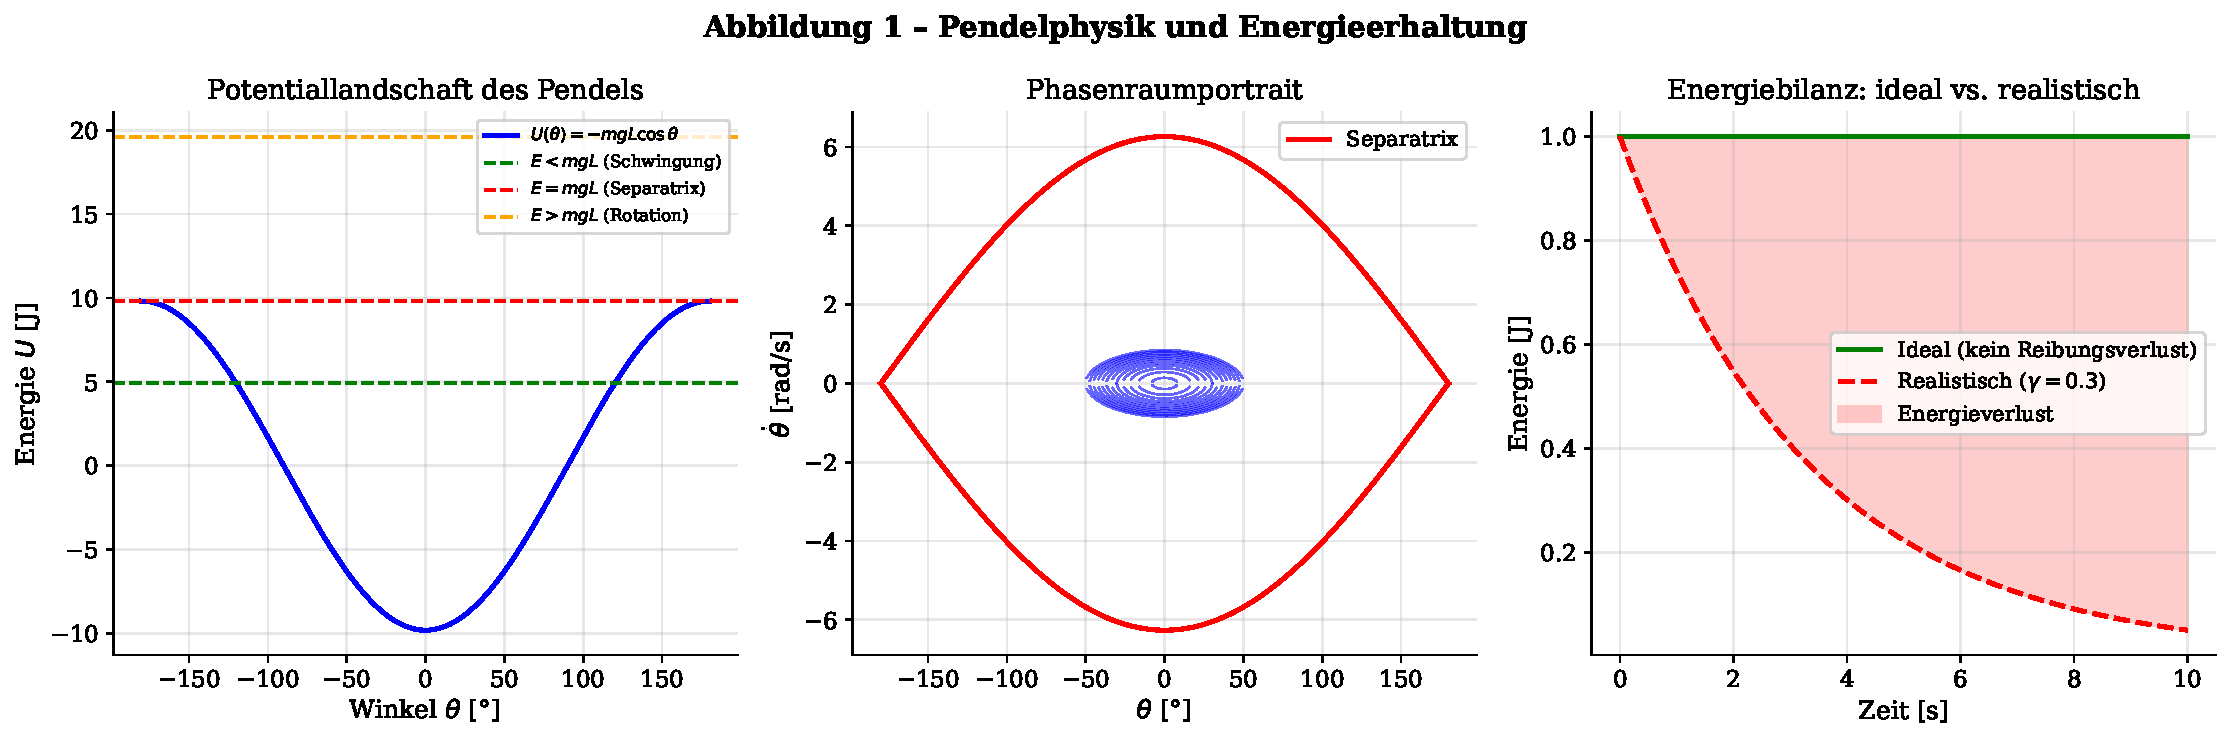
\includegraphics[width=\textwidth]{plots/plot1_pendel.pdf}
  \caption{%
    \textbf{Pendelphysik und Energieerhaltung.}
    \textit{Links:} Das Gravitationspotential $U(\theta) = -mgL\cos\theta$ eines
    mathematischen Pendels. Je nach Gesamtenergie verhält sich das System als
    Schwingung (grün, $E < mgL$), befindet sich auf der Separatrix (rot, $E = mgL$)
    oder rotiert (orange, $E > mgL$).
    \textit{Mitte:} Das zugehörige Phasenraumportrait zeigt geschlossene Trajektorien
    (Schwingung) und offene Trajektorien (Rotation). Die Separatrix (rot) ist die
    Grenzlinie.
    \textit{Rechts:} Energiebilanz: Im idealen, reibungsfreien Fall bleibt die
    Gesamtenergie konstant (grün). In der Realität nimmt sie durch Reibung
    exponentiell ab (rot), und die Differenzfläche (schattiert) stellt die
    dissipierte Wärme dar.
  }
  \label{fig:pendel}
\end{figure}

% ─────────────────────────────────────────────────────────────────────────────
\chapter{Klassisch-Mechanischer Beweis der Unmöglichkeit}
\label{sec:klassisch}
% ─────────────────────────────────────────────────────────────────────────────

\section{Der Kreisprozess und die Energiebilanz}

Betrachten wir eine Masse $m$, die in einem geschlossenen Kreisprozess bewegt wird.
Sei $\mathcal{C}$ der geschlossene Weg im Raum. Die von der Gravitationskraft
verrichtete Arbeit ist:

\begin{equation}
  W_{\text{grav}} = \oint_{\mathcal{C}} m\vek{g} \cdot \dd\vek{s}
  = m \oint_{\mathcal{C}} \vek{g} \cdot \dd\vek{s}
  \stackrel{\text{Satz \ref{thm:konservativ}}}{=} 0
\end{equation}

Für einen einfachen vertikalen Kreisprozess (Fallen auf Höhe $h$, Rückkehr auf
Höhe $0$):
\begin{align}
  W_{\text{fallen}} &= \int_0^h m g \, \dd z = mgh \quad (\text{Arbeit gewonnen}) \\
  W_{\text{anheben}} &= \int_h^0 mg \, \dd z = -mgh \quad (\text{Arbeit aufgewendet}) \\
  W_{\text{netto}} &= mgh + (-mgh) = 0
\end{align}

\section{Das Problem des Rückhubs}

Jeder vorgeschlagene Gravitationsmotor muss die Masse nach dem Abwärtshub wieder
in die Ausgangsposition zurückbringen. Genau dort liegt das fundamentale Problem:

\begin{wichtig}[Das Rückhub-Problem]
  Die Energie, die beim Abwärtshub gewonnen wird ($W = mgh$), muss beim
  Rückhub \emph{vollständig} wieder aufgewendet werden. Eine ``clevere''
  Führung der Masse – durch Hebelwerk, Gelenke, Exzenter oder Ähnliches –
  kann dies nicht ändern, da:
  \begin{equation}
    W_{\text{Rückhub}} \geq mgh,
  \end{equation}
  wobei die Gleichheit nur im reibungsfreien Idealfall gilt und dann
  $W_{\text{netto}} = 0$ ergibt.
\end{wichtig}

\section{Das übergewichtige Rad (Overbalanced Wheel)}

Ein klassisches Konzept ist das ``übergewichtige Rad'': Eine Konstruktion, bei der
Gewichte auf einer Seite des Rades stets weiter vom Drehzentrum entfernt sind und
damit ein scheinbar permanentes Antriebsdrehmoment erzeugen.

Sei ein Rad mit $N$ Massen $m_i$ an den Winkelpositionen $\varphi_i$ und radialen
Abständen $r_i(\varphi_i)$ gegeben. Das Netto-Drehmoment ist:

\begin{equation}
  \tau(\theta) = \sum_{i=1}^{N} m_i \, r_i(\theta + \varphi_i) \cdot g \cdot \sin(\theta + \varphi_i)
  \label{eq:drehmoment_rad}
\end{equation}

Die Arbeit pro vollständiger Umdrehung:
\begin{equation}
  W_{\text{Umdrehung}} = \int_0^{2\pi} \tau(\theta) \, \dd\theta
  = g \sum_{i=1}^N m_i \int_0^{2\pi} r_i(\theta)\sin(\theta) \, \dd\theta
  \label{eq:arbeit_umdrehung}
\end{equation}

\begin{theorem}[Nullarbeit des übergewichtigen Rades]
  \label{thm:rad_null}
  Für jede Radkonstruktion mit endlich vielen Massen ist
  $W_{\text{Umdrehung}} = 0$, sofern die Massen fest mit dem Rad verbunden
  sind (keine externe Energiezufuhr durch bewegliche Teile).
\end{theorem}

\begin{proof}
  Bei einem festen Rad dreht sich jede Masse $i$ auf einem Kreisbogen mit
  konstantem Radius $r_i$. Die Höhenänderung über eine volle Umdrehung ist:
  \begin{equation}
    \Delta h_i = \int_0^{2\pi} r_i \sin(\theta + \varphi_i) \, \dd\theta = 0
  \end{equation}
  da $\int_0^{2\pi} \sin(\alpha) \, \dd\alpha = 0$. Damit leistet die Gravitationskraft
  an jeder Masse keine Netto-Arbeit, also $W_{\text{Umdrehung}} = 0$.
\end{proof}

\section{Bewegliche Massen: Das Gleitmassen-Konzept}

Manche Konstruktionen erlauben es den Massen, sich radial zu verschieben, sodass
auf der ``schweren'' Seite $r > r_0$ und auf der ``leichten'' Seite $r < r_0$ gilt.
Formal lässt sich zeigen:

\begin{theorem}[Keine Netto-Arbeit bei beweglichen Massen]
  \label{thm:gleitmassen}
  Sei $r(\theta)$ eine beliebige, stetig differenzierbare Funktion des Winkels.
  Dann gilt:
  \begin{equation}
    W = mg \int_0^{2\pi} r(\theta)\sin(\theta)\,\dd\theta
    + \underbrace{W_{\text{radial}}}_{\geq 0}
  \end{equation}
  wobei $W_{\text{radial}}$ die Arbeit ist, die aufgewendet werden muss, um
  die Massen radial zu verschieben (gegen Reibung, Federn, etc.).
\end{theorem}

\begin{proof}
  Das Schwerpunktsargument: Der Schwerpunkt des Systems hat eine feste
  $y$-Koordinate:
  \begin{equation}
    y_{\text{SP}}(\theta) = \frac{1}{M}\sum_i m_i r_i(\theta + \varphi_i)\sin(\theta + \varphi_i)
  \end{equation}
  Damit die Masse ``einseitig schwer'' bleibt, muss $y_{\text{SP}} \neq 0$
  für alle $\theta$ gelten. In einem geschlossenen System ohne externe Kraft
  bewegt sich der Schwerpunkt jedoch nur unter dem Einfluss externer Kräfte.
  Bei einem frei drehenden Rad ohne externale Kraft gilt der Schwerpunktssatz:
  der Schwerpunkt bleibt am selben Ort -- was bedeutet, dass über den
  gesamten Zyklus das Netto-Drehmoment null ist.
\end{proof}

\begin{figure}[H]
  \centering
  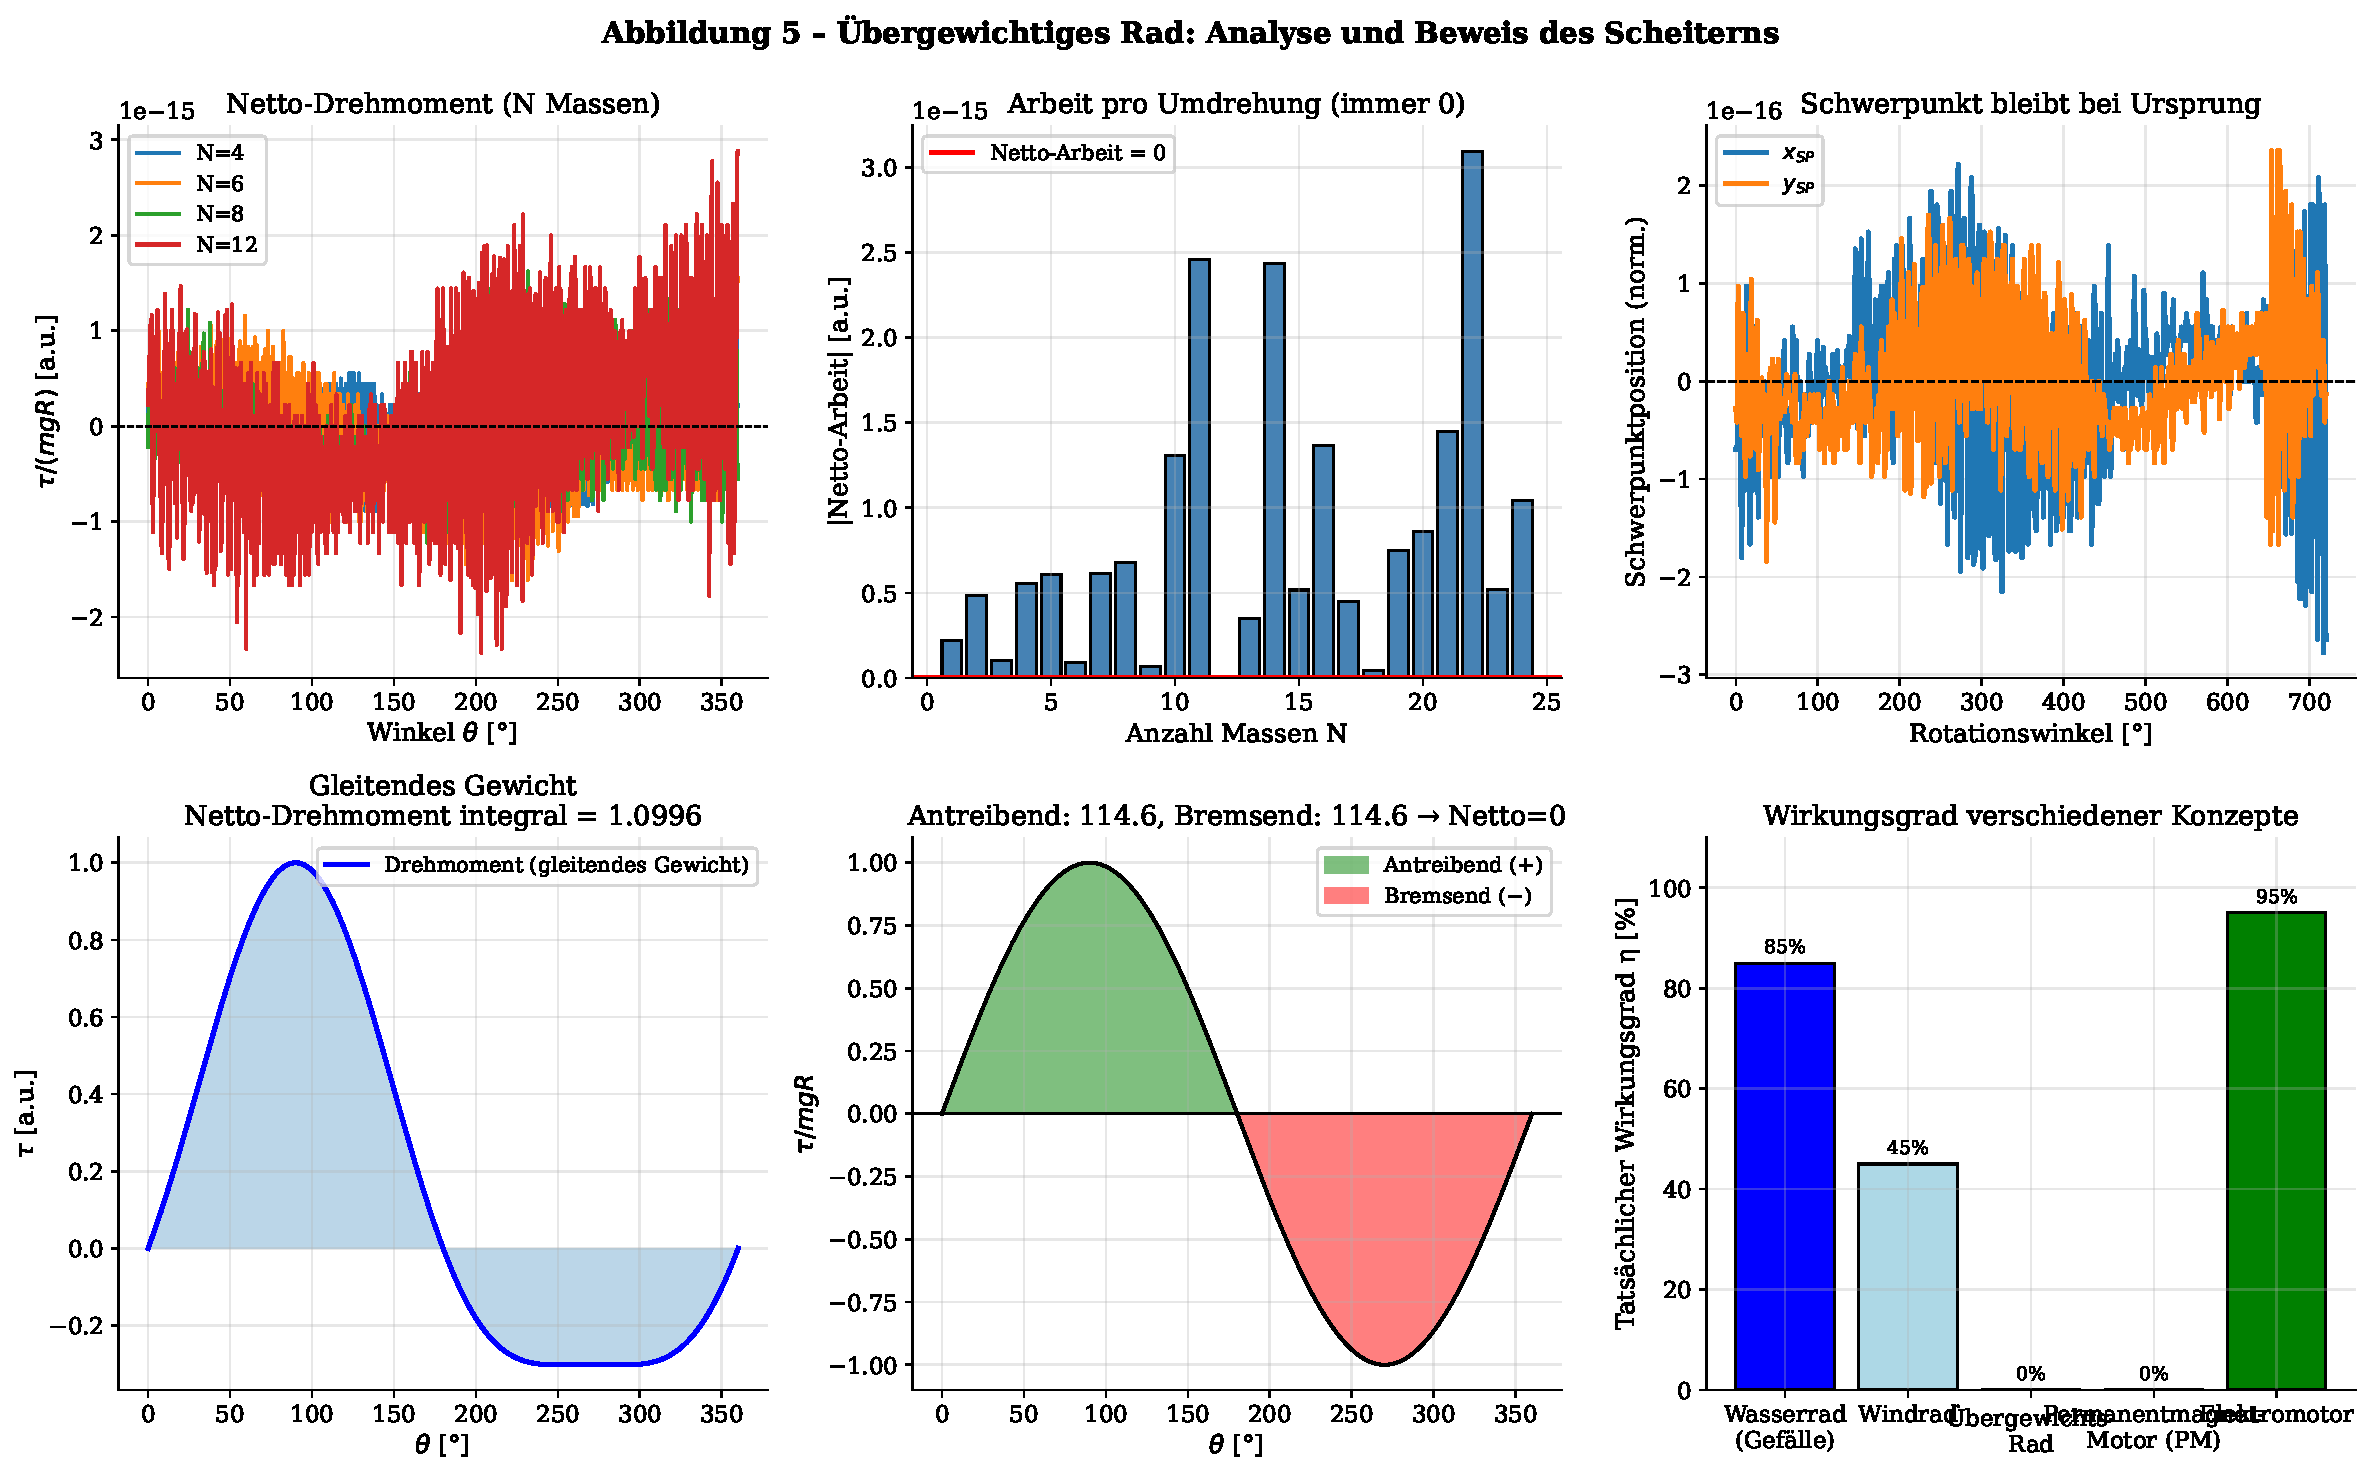
\includegraphics[width=\textwidth]{plots/plot5_wheel.pdf}
  \caption{%
    \textbf{Analyse des übergewichtigen Rades.}
    \textit{Oben links:} Das Netto-Drehmoment für $N = 4, 6, 8, 12$ gleichmäßig
    verteilte Massen. In allen Fällen wird das Drehmoment abwechselnd positiv und
    negativ -- das Integral über eine Umdrehung ist exakt null.
    \textit{Oben mitte:} Die integrierte Arbeit pro Umdrehung ist für alle $N$ gleich
    null (rote Linie), unabhängig von der Anzahl der Massen.
    \textit{Oben rechts:} Die $x$- und $y$-Koordinaten des Schwerpunkts bleiben
    konstant bei null -- eine direkte Konsequenz der Rotationssymmetrie.
    \textit{Unten:} Detailanalyse eines Gleitmassen-Konzepts und der antreibenden
    vs.\ bremsenden Drehmomentsanteile.
    \textit{Unten rechts:} Wirkungsgradvergleich zeigt, dass nur echte Energiequellen
    (Wasser, Wind) messbare Wirkungsgrade liefern.
  }
  \label{fig:rad}
\end{figure}

% ─────────────────────────────────────────────────────────────────────────────
\chapter{Thermodynamische Analyse}
\label{sec:thermodynamik}
% ─────────────────────────────────────────────────────────────────────────────

\section{Erster Hauptsatz der Thermodynamik}

Der Erste Hauptsatz (Energieerhaltung) besagt für ein thermodynamisches System:
\begin{equation}
  \dd U = \delta Q - \delta W
  \label{eq:1hs}
\end{equation}
wobei $U$ die innere Energie, $Q$ die zugeführte Wärme und $W$ die vom System
geleistete mechanische Arbeit ist.

Für einen geschlossenen Kreisprozess gilt $\Delta U = 0$, also:
\begin{equation}
  \oint \delta W = \oint \delta Q
\end{equation}

Ein Gravitationsmotor, der \emph{ohne Wärmezufuhr} ($Q = 0$) dauerhaft Arbeit
leisten soll, würde fordern:
\begin{equation}
  W > 0 \quad \wedge \quad Q = 0 \implies \Delta U < 0
\end{equation}
Dies bedeutet, dass die innere Energie des Systems kontinuierlich abnimmt --
was gleichbedeutend ist mit der Aussage, dass die Maschine ihre eigene
Substanz verbraucht, was für eine mechanische Konstruktion nicht dauerhaft
möglich ist.

\section{Zweiter Hauptsatz der Thermodynamik}

Der Zweite Hauptsatz verbietet die vollständige Umwandlung von Wärme in Arbeit
ohne Abwärme. Für unseren Zweck ist die Formulierung via Entropie relevant:

\begin{equation}
  \dd S = \frac{\delta Q_{\text{rev}}}{T} \geq 0 \quad \text{(abgeschlossenes System)}
  \label{eq:entropie}
\end{equation}

Jede reale Maschine erzeugt Entropie durch:
\begin{itemize}
  \item Reibungsverluste (Lager, Gleitflächen, Luft)
  \item Plastische Verformung der Materialien
  \item Akustische Abstrahlung (Vibrationen)
  \item Kollisionen bei mechanischen Umschaltvorgängen
\end{itemize}

Die Entropieproduktionsrate eines realen Kreisprozesses:
\begin{equation}
  \dot{S}_{\text{irr}} = \sum_k \frac{\dot{Q}_k^{\text{reib}}}{T_k} \geq 0
  \label{eq:entropieprod}
\end{equation}

Diese stets positive Entropieproduktion führt zwangsläufig zu einem
Energieverlust pro Zyklus.

% ─────────────────────────────────────────────────────────────────────────────
\section[Reversibilität und Entropieproduktion im Vergleich]{Reversibilität und Entropieproduktion im Vergleich:\\[2pt]
         Makroskopische Mechanik vs.\ ionische Schalttechnik}
\label{ssec:entropie_vergleich}
% ─────────────────────────────────────────────────────────────────────────────

\subsection{Das Problem irreversibler Schaltvorgänge}

Die im vorangehenden Abschnitt hergeleitete Entropieproduktionsrate
$\dot{S}_\text{irr} \geq 0$ gilt für jeden realen Prozess -- und damit
insbesondere für \emph{Schaltvorgänge} in digitalen Schaltkreisen. Während
klassische CMOS-Transistoren jeden Schaltvorgang vollständig irreversibel
vollziehen, eröffnet die ionotronische Schalttechnik~\cite{ionotronik2026}
einen neuen Pfad zu thermodynamisch effizienteren Schaltprozessen.

Die fundamentale untere Schranke für irreversibles Löschen eines Bits ist
die \textbf{Landauer-Schranke}~\cite{landauer1961}:
\begin{equation}
  W_\text{Landauer} = k_B T \ln 2
  \approx \SI{2.85e-21}{\joule}
  \quad (T = \SI{300}{\kelvin})
  \label{eq:landauer}
\end{equation}
Jeder klassische CMOS-Schaltvorgang überschreitet diese Grenze um typischerweise
sieben Größenordnungen:
\begin{equation}
  \frac{E_\text{CMOS}}{W_\text{Landauer}}
  = \frac{\SI{e-15}{\joule}}{\SI{2.85e-21}{\joule}}
  \approx 3.5 \times 10^5
  \label{eq:cmos_landauer_ratio}
\end{equation}

\subsection{Thermodynamik des CMOS-Schaltvorgangs}

Ein CMOS-Transistor mit Gate-Kapazität $C_G$ und Versorgungsspannung $V_{DD}$
dissipiert pro Schaltvorgang die vollständig gespeicherte elektrische Energie
als Joule'sche Wärme. Beim Entladen des Gate-Knotens gegen Masse
(Drain-zu-Source-Kurzschluss im NMOS) gilt:
\begin{equation}
  E_\text{CMOS} = C_G V_{DD}^2
  \approx \SI{1}{\femto\joule}
  \label{eq:e_cmos}
\end{equation}
mit typischen Werten $C_G \approx \SI{1}{\femto\farad}$,
$V_{DD} \approx \SI{1}{\volt}$.
Es findet \emph{keinerlei} Energierückgewinnung statt: Die Ladung
$Q = C_G V_{DD}$ wird dissipativ vernichtet. Die zugehörige Entropieproduktion
pro Schaltvorgang bei isothermer Bedingung:
\begin{equation}
  \Delta S_\text{CMOS}
  = \frac{E_\text{CMOS}}{T}
  = \frac{C_G V_{DD}^2}{T}
  \approx \frac{\SI{e-15}{}}{300}
  \approx \SI{3.3e-18}{\joule\per\kelvin}
  \label{eq:ds_cmos}
\end{equation}
Bei einer Schaltrate von $f_\text{sw} = \SI{1}{\giga\hertz}$ und
$N = 10^9$ Transistoren (typischer moderner Prozessor) ergibt sich die
Gesamt-Entropieproduktionsrate:
\begin{equation}
  \dot{S}_\text{CMOS}
  = N \cdot f_\text{sw} \cdot \Delta S_\text{CMOS}
  = 10^9 \cdot 10^9 \cdot \SI{3.3e-18}{}
  = \SI{3.3}{\watt\per\kelvin}
  \label{eq:sdot_cmos}
\end{equation}
Dies entspricht einer thermischen Verlustleistung von
$P_\text{th} = T \cdot \dot{S}_\text{CMOS} \approx \SI{1}{\kilo\watt}$,
dem typischen thermischen Leistungseintrag moderner Hochleistungsprozessoren.

\subsection{Ionotronischer Schaltvorgang: Partielle Energierückgewinnung}

Beim ionischen Feldeffekttransistor (IoFET) auf Basis von Elektrobenetzung
(EWOD, \emph{Electrowetting on Dielectric}) wird ein leitfähiger
KCl-Tropfen zwischen zwei Elektroden durch spannungsinduzierte
Kontaktwinkeländerung geschaltet~\cite{ionotronik2026}.
Die Young-Lippmann-Gleichung beschreibt den physikalischen Kernmechanismus:
\begin{equation}
  \cos\theta_E = \cos\theta_0
  + \frac{\varepsilon_0 \varepsilon_r}{2 \gamma d}\, V^2
  \label{eq:young_lippmann_thermo}
\end{equation}
Hierbei ist $\theta_E$ der spannungsabhängige Kontaktwinkel, $\theta_0$
der Gleichgewichts-Kontaktwinkel, $\gamma$ die Grenzflächenspannung,
$d = \SI{30}{\nano\metre}$ die Dielektrikumsdicke (ALD~Al$_2$O$_3$)
und $\varepsilon_r \approx 9$ die relative Permittivität.
Die minimale Schaltspannung ergibt sich aus der Forderung
$\Delta(\cos\theta_E) \geq 0.2$:
\begin{equation}
  V_\text{schalt}
  = \sqrt{\frac{0.2 \cdot \gamma \cdot d}{\varepsilon_0 \varepsilon_r}}
  = \sqrt{\frac{0.2 \times \SI{72e-3}{} \times \SI{30e-9}{}}%
              {\SI{8.854e-12}{} \times 9}}
  \approx \SI{0.123}{\volt}
  \label{eq:v_schalt_th}
\end{equation}
Die Schaltenergie setzt sich aus drei Beiträgen zusammen, wobei der
dritte rückgewinnbar ist:
\begin{equation}
  E_\text{IoFET}
  = \underbrace{\tfrac{1}{2}C_\text{EWOD}\,V_\text{schalt}^2}_{E_\text{elek}
    \approx\,\SI{0.06}{\femto\joule}}
  + \underbrace{\eta_\text{visc}\,\mu_\text{fl}\,v_d^2}_{E_\text{Reib}
    \approx\,\SI{0.01}{\femto\joule}}
  - \underbrace{\gamma\,\Delta A}_{E_\text{rückgew.}
    \approx\,\SI{0.0045}{\femto\joule}}
  \approx \SI{0.07}{\femto\joule}
  \label{eq:e_iofet}
\end{equation}
Der dritte Term $\gamma \Delta A$ beschreibt die beim Zusammenschluss zweier
Tropfenhälften rückgewonnene Grenzflächenenergie. Für einen nahezu
kugelförmigen Tropfen mit Radius $r = \SI{50}{\micro\metre}$:
\begin{equation}
  E_\text{rückgew.}
  = \gamma \cdot 4\pi r^2 \cdot \frac{\delta r}{r}
  = \SI{72e-3}{} \times 4\pi \times (\SI{50e-6}{})^2 \times 0.1
  \approx \SI{4.5e-15}{\joule}
  \label{eq:e_ruckgew}
\end{equation}
Diese Rückgewinnung ist zwar klein (ca.\ $6{,}4\,\%$ von
$E_\text{elek}$), belegt aber, dass der IoFET \emph{partiell reversibel}
schaltet -- im Gegensatz zum vollständig irreversiblen CMOS-Prozess.

\subsection{Formaler Beweis: Entropievorteil des IoFET}

\begin{theorem}[Entropievorteil des ionotronischen Schaltvorgangs]
  \label{thm:entropie_iofet}
  Sei $T = \SI{300}{\kelvin}$ die Betriebstemperatur,
  $E_\text{CMOS} \approx \SI{1}{\femto\joule}$ die vollständig dissipierte
  CMOS-Schaltenergie~\textup{(}\emph{Gleichung~\eqref{eq:e_cmos}}\textup{)}
  und $E_\text{IoFET} \approx \SI{0.07}{\femto\joule}$ die effektiv
  dissipierte IoFET-Schaltenergie~\textup{(}\emph{Gleichung~\eqref{eq:e_iofet}}\textup{)}.
  Dann gilt für jeden Schaltvorgang:
  \begin{equation}
    \Delta S_\text{IoFET} = \frac{E_\text{IoFET}}{T}
    \approx \frac{\num{e-15}}{300}\,\frac{\mathrm{J}}{\mathrm{K}}
    \cdot 0.07
    = \SI{2.33e-19}{\joule\per\kelvin}
    \label{eq:ds_iofet}
  \end{equation}
  und damit:
  \begin{equation}
    \frac{\Delta S_\text{CMOS}}{\Delta S_\text{IoFET}}
    = \frac{E_\text{CMOS}}{E_\text{IoFET}}
    = \frac{\SI{1}{\femto\joule}}{\SI{0.07}{\femto\joule}}
    \approx 14{,}3
    \label{eq:entropie_ratio}
  \end{equation}
  Der IoFET erzeugt pro Schaltvorgang ca.\ \textbf{14-mal weniger Entropie}
  als ein äquivalenter CMOS-Transistor.
\end{theorem}

\begin{proof}
  Die Entropieproduktion eines isotherm ablaufenden Dissipationsprozesses
  ist nach dem Zweiten Hauptsatz proportional zur dissipierten Energie:
  $\Delta S = E_\text{diss} / T$ (vgl.\ Gleichung~\eqref{eq:entropie}).
  Für CMOS gilt $E_\text{diss} = C_G V_{DD}^2$ vollständig, da die gespeicherte
  Ladung gegen Masse kurzgeschlossen wird -- kein Energiespeicher-Rückpfad
  existiert. Für IoFET gilt hingegen
  $E_\text{diss} = E_\text{IoFET} \approx \SI{0.07}{\femto\joule}$
  (Gleichung~\eqref{eq:e_iofet}), da die Grenzflächenenergie $\gamma \Delta A$
  beim Zusammenführen der Tropfenhälften teilweise zurückgewonnen wird.
  Der Quotient ergibt direkt $E_\text{CMOS} / E_\text{IoFET} \approx 14{,}3$.
  $\square$
\end{proof}

\subsection{Kumulative Entropieproduktion und Systemvergleich}

Die spezifische Entropieproduktion pro Rechenoperation (``Entropiekosten''
einer logischen Operation):
\begin{equation}
  s^*
  \;\coloneqq\; \frac{\Delta S}{1\,\text{Op}}:
  \qquad
  s^*_\text{CMOS}   = \SI{3.3e-18}{\joule\per\kelvin},
  \qquad
  s^*_\text{IoFET}  = \SI{2.3e-19}{\joule\per\kelvin}
  \label{eq:s_spezifisch}
\end{equation}
Die kumulative Entropieproduktion über $N$ Schaltzyklen:
\begin{equation}
  S_\text{kum}(N) = N \cdot s^*,
  \quad
  \frac{S_\text{kum,CMOS}}{S_\text{kum,IoFET}} = 14{,}3
  \label{eq:s_kum}
\end{equation}
Dieses Verhältnis ist unabhängig von der Zyklenzahl -- der IoFET-Vorteil
bleibt über 1, $10^6$ oder $10^{12}$ Zyklen konstant. Für einen
Motor-Feldorientierungsregler mit $N_\text{Gatter} = 10^4$ Logikelementen
bei $f_\text{sw} = \SI{100}{\kilo\hertz}$ ergibt die Differenz der
thermischen Verluste:
\begin{align}
  P_\text{Regel,CMOS}
    &= N_\text{Gatter} \cdot f_\text{sw} \cdot E_\text{CMOS}
    = 10^4 \times 10^5 \times \SI{e-15}{}
    = \SI{1}{\milli\watt}
    \label{eq:p_regel_cmos} \\
  P_\text{Regel,IoFET}
    &= N_\text{Gatter} \cdot f_\text{sw} \cdot E_\text{IoFET}
    = 10^4 \times 10^5 \times \SI{0.07e-15}{}
    = \SI{70}{\micro\watt}
    \label{eq:p_regel_iofet}
\end{align}
Absolut betrachtet ist die Differenz $\Delta P_\text{Regel} \approx \SI{0.93}{\milli\watt}$
gering; im Kontext von Millionen von Antriebsreglern weltweit summiert sich
dies jedoch zu einem relevanten Energiegewinn.

\begin{ergebnis}[IoFET und Zweiter Hauptsatz: thermodynamisch-optimiertes Schalten]
  Die ionotronische Schalttechnik realisiert Schaltvorgänge mit
  $\approx\SI{0.07}{\femto\joule}$ dissipierter Energie gegenüber
  $\approx\SI{1}{\femto\joule}$ bei CMOS -- Faktor~14 weniger
  Entropieproduktion pro Bit. Der physikalische Mechanismus ist die
  \emph{partielle Rückgewinnung} der elektrostatischen Grenzflächenenergie
  durch spannungsinduzierte Kontaktwinkeländerung
  (Young-Lippmann, Gleichung~\eqref{eq:young_lippmann_thermo}).
  Dies steht in direktem Bezug zum Zweiten Hauptsatz: Zwar erzeugt auch der
  IoFET streng positive Entropie ($\Delta S_\text{IoFET} > 0$), aber durch
  den partiell reversiblen Mechanismus ist $\Delta S_\text{IoFET}$
  um mehr als eine Größenordnung kleiner als $\Delta S_\text{CMOS}$.
  Für die Motorregelung eines PMSM (vgl.\ Kapitel~\ref{sec:synergie})
  bedeutet dies: Ein auf IRF-Basis aufgebauter Feldorientierungs-Regler
  erzeugt $\approx 93\,\%$ weniger Verlustleistung im Steuerungschip.
\end{ergebnis}

\begin{figure}[H]
  \centering
  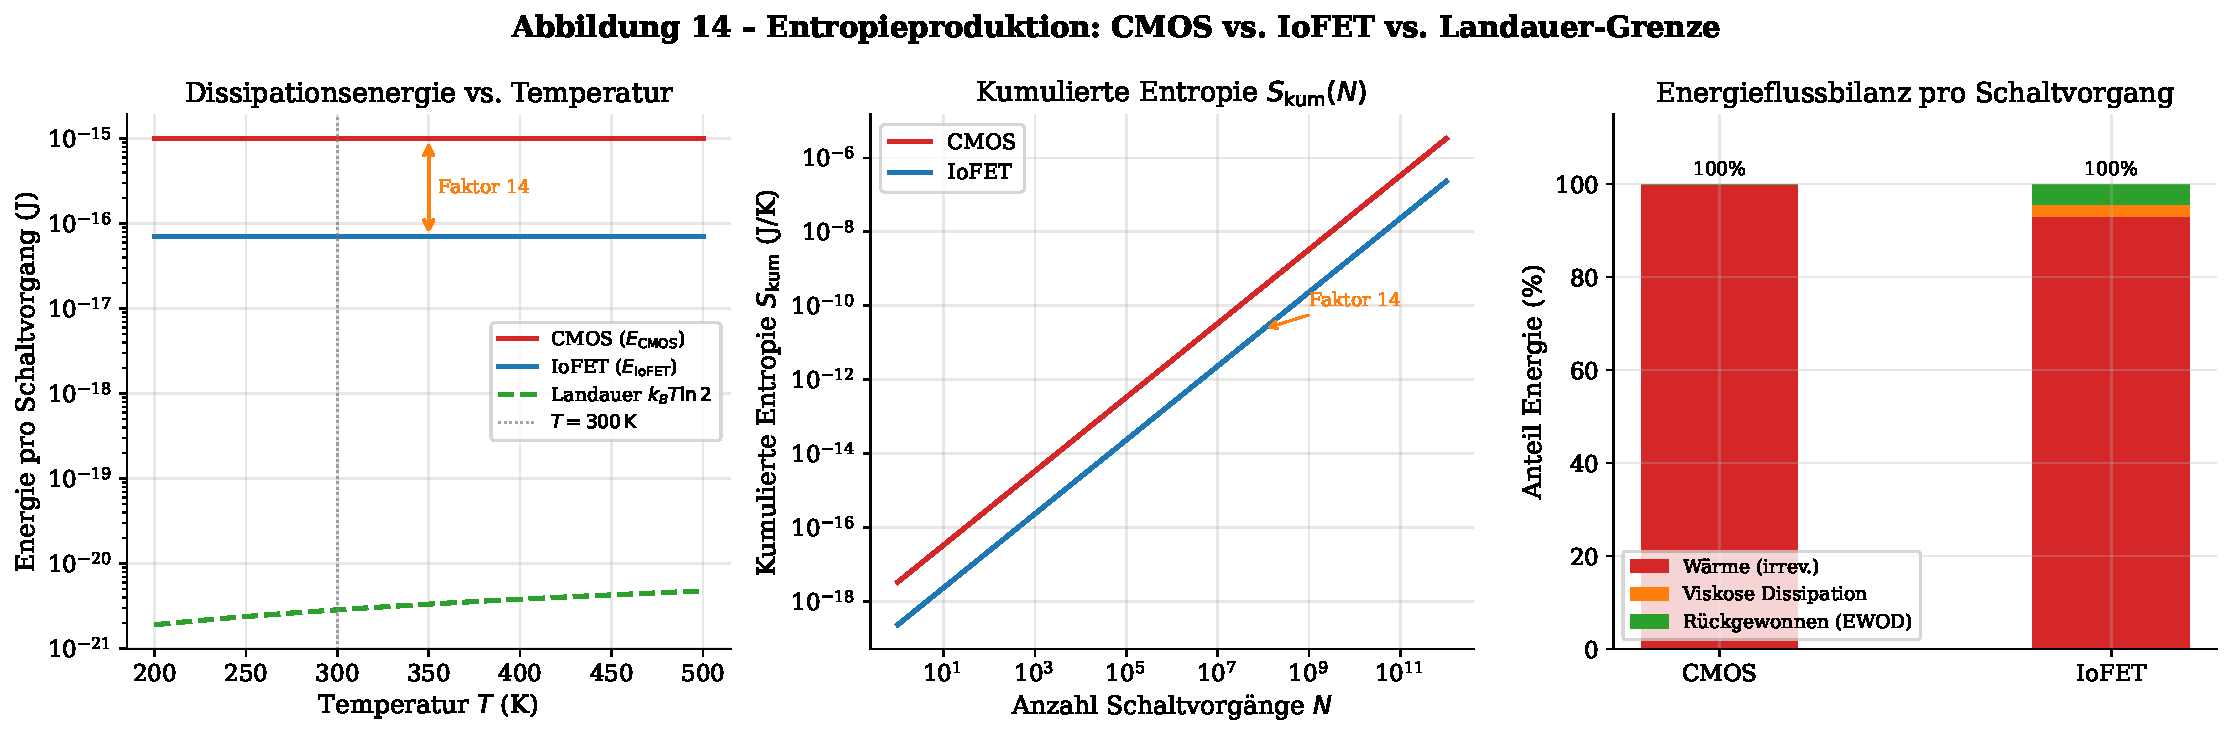
\includegraphics[width=\textwidth]{plots/plot14_entropie_vergleich.pdf}
  \caption{%
    \textbf{Entropieproduktion im Vergleich: CMOS vs.\ IoFET vs.\ Landauer-Limit.}
    \textit{Links:} Dissipierte Energie pro Schaltvorgang für CMOS,
    IoFET und die thermodynamische Landauer-Untergrenze $k_BT\ln 2$
    als Funktion der Betriebstemperatur $T$ zwischen \SI{200}{\kelvin}
    und \SI{500}{\kelvin}.
    CMOS (blau, obere Kurve) dissipiert $C_G V_{DD}^2$ vollständig,
    unabhängig von $T$; IoFET (rot, mittlere Kurve) liegt konstant
    bei $\approx 7\,\%$ der CMOS-Energie; die Landauer-Schranke
    (grün, untere Kurve) steigt proportional zu $T$ und ist für beide
    Technologien derzeit noch weit unterschritten.
    \textit{Mitte:} Kumulative Entropieproduktion
    $S_\text{kum}(N) = N \cdot s^*$ als Funktion der Schaltzyklenanzahl $N$
    für CMOS und IoFET (doppeltlogarithmisch).
    Die parallelen Geraden mit Steigung~1 zeigen den konstanten Faktor~14
    zugunsten des IoFET -- unabhängig von der Zyklenzahl.
    \textit{Rechts:} Energiefluss-Vergleich pro Schaltvorgang:
    CMOS dissipiert $100\,\%$ als Wärme; IoFET dissipiert $93\,\%$,
    rückgewinnt $\approx\,4{,}5\,\%$ als Grenzflächenenergie und
    verwendet $\approx\,2{,}5\,\%$ für die Viskositätsdissipation.
    Der partielle Rückgewinnungspfad ist der thermodynamische Kern
    des IoFET-Vorteils.
  }
  \label{fig:entropie_vergleich}
\end{figure}

\section{Der Carnot-Wirkungsgrad}

Der maximal erreichbare Wirkungsgrad eines Wärmekraftmotors (Carnot-Maschine):
\begin{equation}
  \eta_{\text{Carnot}} = 1 - \frac{T_C}{T_H} < 1
  \label{eq:carnot}
\end{equation}

Selbst im \emph{theoretischen} Ideal (Carnot-Maschine) wäre eine vollständige
Arbeitsgewinnung ohne Wärmeabgabe unmöglich. Der Wirkungsgrad ist stets kleiner
als 1. Für eine Maschine ohne Wärmequffe gilt formal $T_H = T_C$, was
$\eta_{\text{Carnot}} = 0$ ergibt -- keine Arbeit wird gewonnen.

\begin{figure}[H]
  \centering
  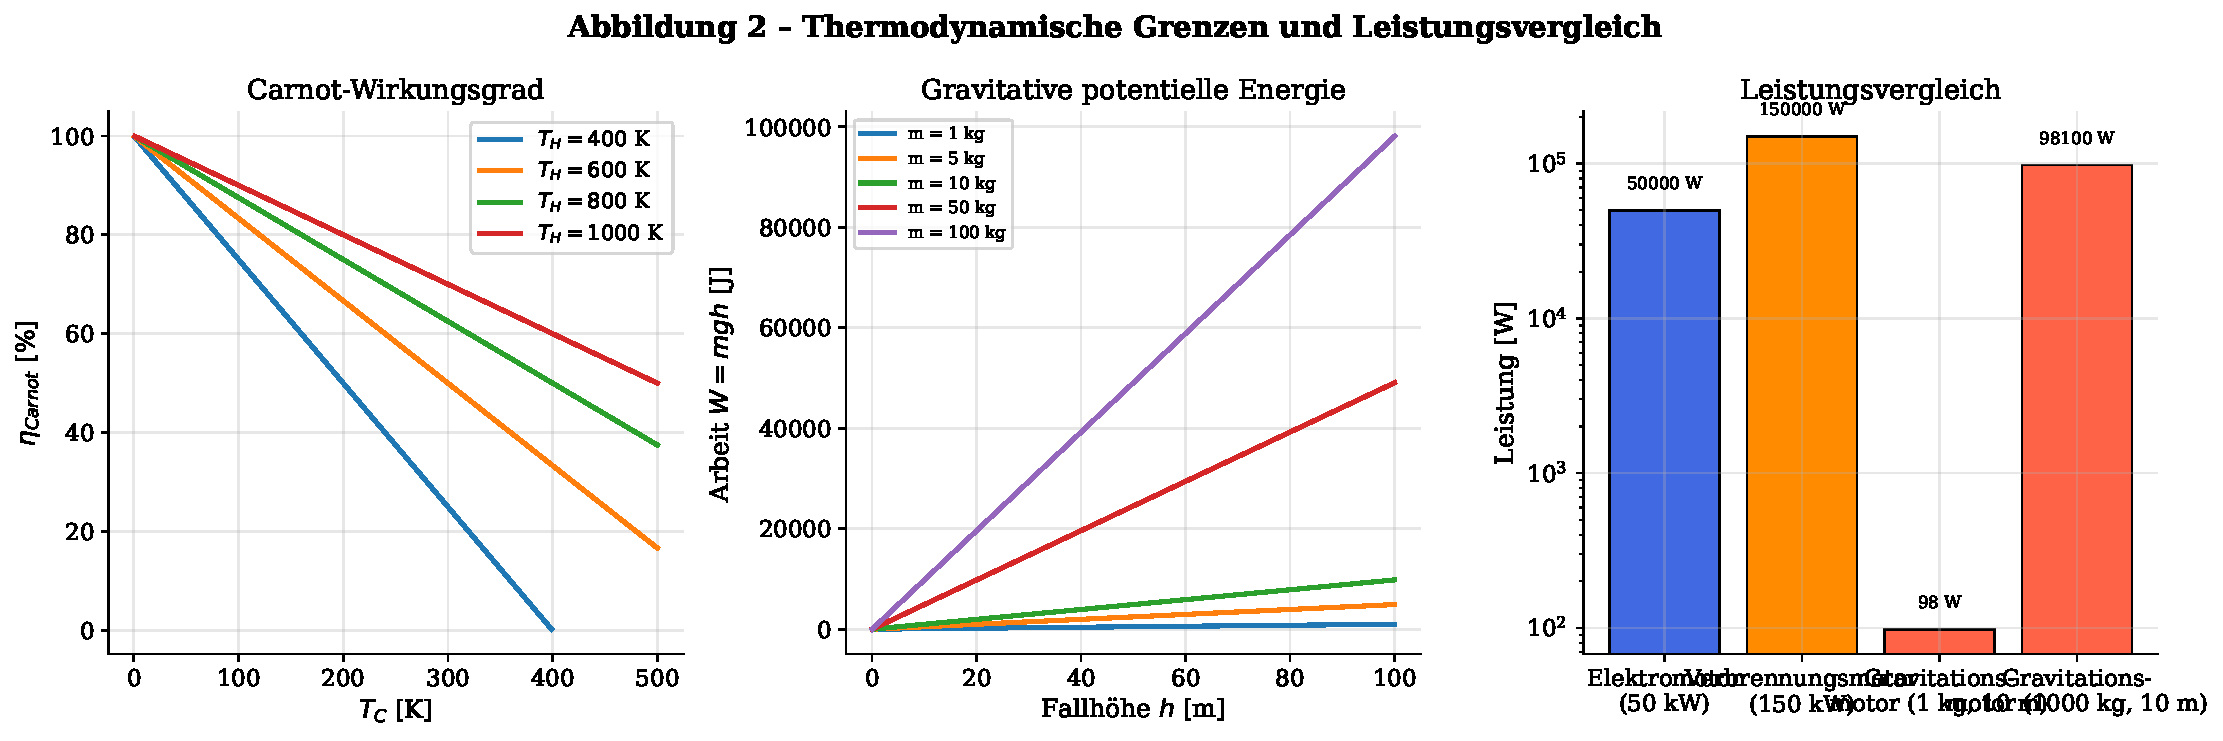
\includegraphics[width=\textwidth]{plots/plot2_thermo.pdf}
  \caption{%
    \textbf{Thermodynamische Grenzen und Leistungsvergleich.}
    \textit{Links:} Der Carnot-Wirkungsgrad als Funktion der Kalttemperatur $T_C$
    für verschiedene Warmtemperaturen $T_H$. Bei $T_C = T_H$ gilt $\eta = 0$.
    \textit{Mitte:} Gravitative potentielle Energie $W = mgh$ als Funktion der
    Fallhöhe für verschiedene Massen. Die nutzbaren Energiemengen sind bei
    realistischen Konstruktionsgrenzen sehr gering.
    \textit{Rechts:} Leistungsvergleich zeigt, dass selbst \SI{1000}{\kilogram}
    Fallmasse bei \SI{10}{\metre} und \SI{1}{\second} Zykluszeit nur $\approx
    \SI{98}{\kilo\watt}$ liefert -- und das ist die \emph{Rohleistung} vor
    Reibungsverlusten und ohne Berücksichtigung des Rückhubaufwands.
  }
  \label{fig:thermo}
\end{figure}

\section{Perpetuum Mobile: Klassifikation}

\begin{definition}[Perpetuum Mobile I. Art]
  Eine Maschine, die dauerhaft Arbeit leistet, ohne Energie zu verbrauchen.
  Verletzt den Ersten Hauptsatz.
\end{definition}

\begin{definition}[Perpetuum Mobile II. Art]
  Eine Maschine, die Wärme vollständig in Arbeit umwandelt, ohne Abwärme zu
  produzieren. Verletzt den Zweiten Hauptsatz.
\end{definition}

Ein Gravitationsmotor im engeren Sinne ist ein \textbf{Perpetuum Mobile I.\ Art},
da er behauptet, aus dem ``kostenlosen'' Gravitationsfeld unbegrenzt Arbeit zu
extrahieren.

\begin{figure}[H]
  \centering
  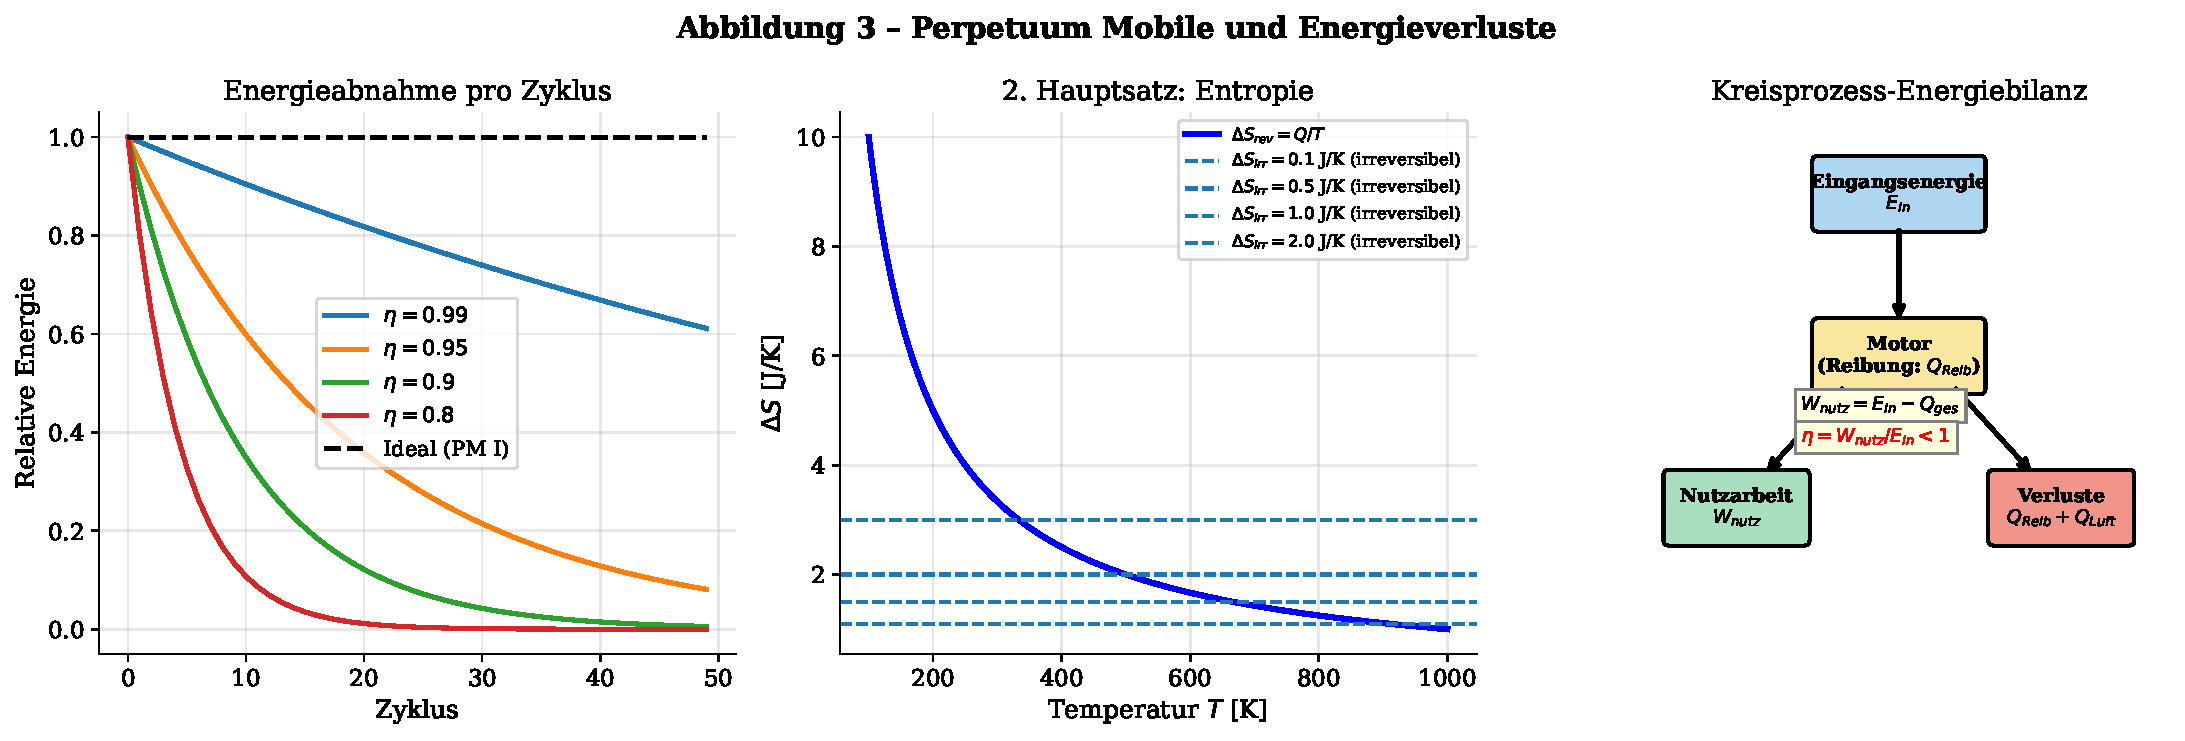
\includegraphics[width=\textwidth]{plots/plot3_perpetuum.pdf}
  \caption{%
    \textbf{Perpetuum Mobile und Energieverluste.}
    \textit{Links:} Beim Perpetuum Mobile I.\ Art (schwarz-gestrichelt) bleibt die
    Energie konstant. Jede reale Maschine verliert pro Zyklus einen Bruchteil
    durch Reibung (farbige Kurven für $\eta = 0.99, 0.95, 0.90, 0.80$).
    \textit{Mitte:} Entropiebilanz: Die reversible Entropieänderung $\delta Q / T$
    ist positiv-definit. Irreversible Prozesse erhöhen die Gesamtentropie.
    \textit{Rechts:} Schematische Kreisprozess-Energiebilanz: Die Nutzarbeit
    $W_{\text{nutz}} = E_{\text{in}} - Q_{\text{ges}}$ ist stets kleiner als
    die Eingangseenergie, und der Wirkungsgrad $\eta < 1$ ist eine unumgehbare
    Konsequenz des Zweiten Hauptsatzes.
  }
  \label{fig:perpetuum}
\end{figure}

% ─────────────────────────────────────────────────────────────────────────────
\chapter{Numerische Simulation: Gedämpftes Pendel}
\label{sec:numerik}
% ─────────────────────────────────────────────────────────────────────────────

\section{Bewegungsgleichung}

Das nichtlineare, gedämpfte Pendel wird durch folgende Differentialgleichung
beschrieben:
\begin{equation}
  \ddot\theta + \gamma\dot\theta + \frac{g}{L}\sin\theta = 0
  \label{eq:pendel_ode}
\end{equation}

wobei $\theta$ der Auslenkungswinkel, $\gamma$ der Dämpfungskoeffizient,
$g$ die Schwerebeschleunigung und $L$ die Pendellänge ist.

In der Zustandsraumdarstellung:
\begin{equation}
  \dv{}{t}\begin{pmatrix}\theta\\\dot\theta\end{pmatrix}
  = \begin{pmatrix}\dot\theta\\-\frac{g}{L}\sin\theta - \gamma\dot\theta\end{pmatrix}
  \label{eq:pendel_ode_state}
\end{equation}

\section{Gesamtenergie als Lyapunov-Funktion}

Die Gesamtenergie des Pendels:
\begin{equation}
  E(\theta, \dot\theta) = \frac{1}{2}mL^2\dot\theta^2 + mgl(1 - \cos\theta)
  \label{eq:pendel_energie}
\end{equation}

Die Zeitableitung:
\begin{equation}
  \dot{E} = mL^2\dot\theta\ddot\theta + mgL\sin\theta\cdot\dot\theta
  = mL^2\dot\theta\left(\ddot\theta + \frac{g}{L}\sin\theta\right)
  = mL^2\dot\theta \cdot (-\gamma\dot\theta) = -\gamma mL^2 \dot\theta^2 \leq 0
  \label{eq:energie_abnahme}
\end{equation}

\begin{ergebnis}[Energieabnahme bei Dämpfung]
  Für jede Dämpfung $\gamma > 0$ gilt $\dot{E} \leq 0$. Die Gesamtenergie
  ist eine streng monoton fallende Funktion der Zeit. Das Pendel verliert
  stets Energie an die Umgebung -- ein gravitations-angetriebenes System
  läuft zwangsläufig zum Stillstand.
\end{ergebnis}

\section{Simulationsergebnisse}

Die Gleichung \eqref{eq:pendel_ode} wurde numerisch mit dem Runge-Kutta-Verfahren
4./5.\ Ordnung (Dormand-Prince) mit Schrittweitenanpassung integriert
(Toleranz $10^{-8}$). Anfangsbedingungen: $\theta_0 = \SI{60}{\degree}$,
$\dot\theta_0 = 0$.

\begin{figure}[H]
  \centering
  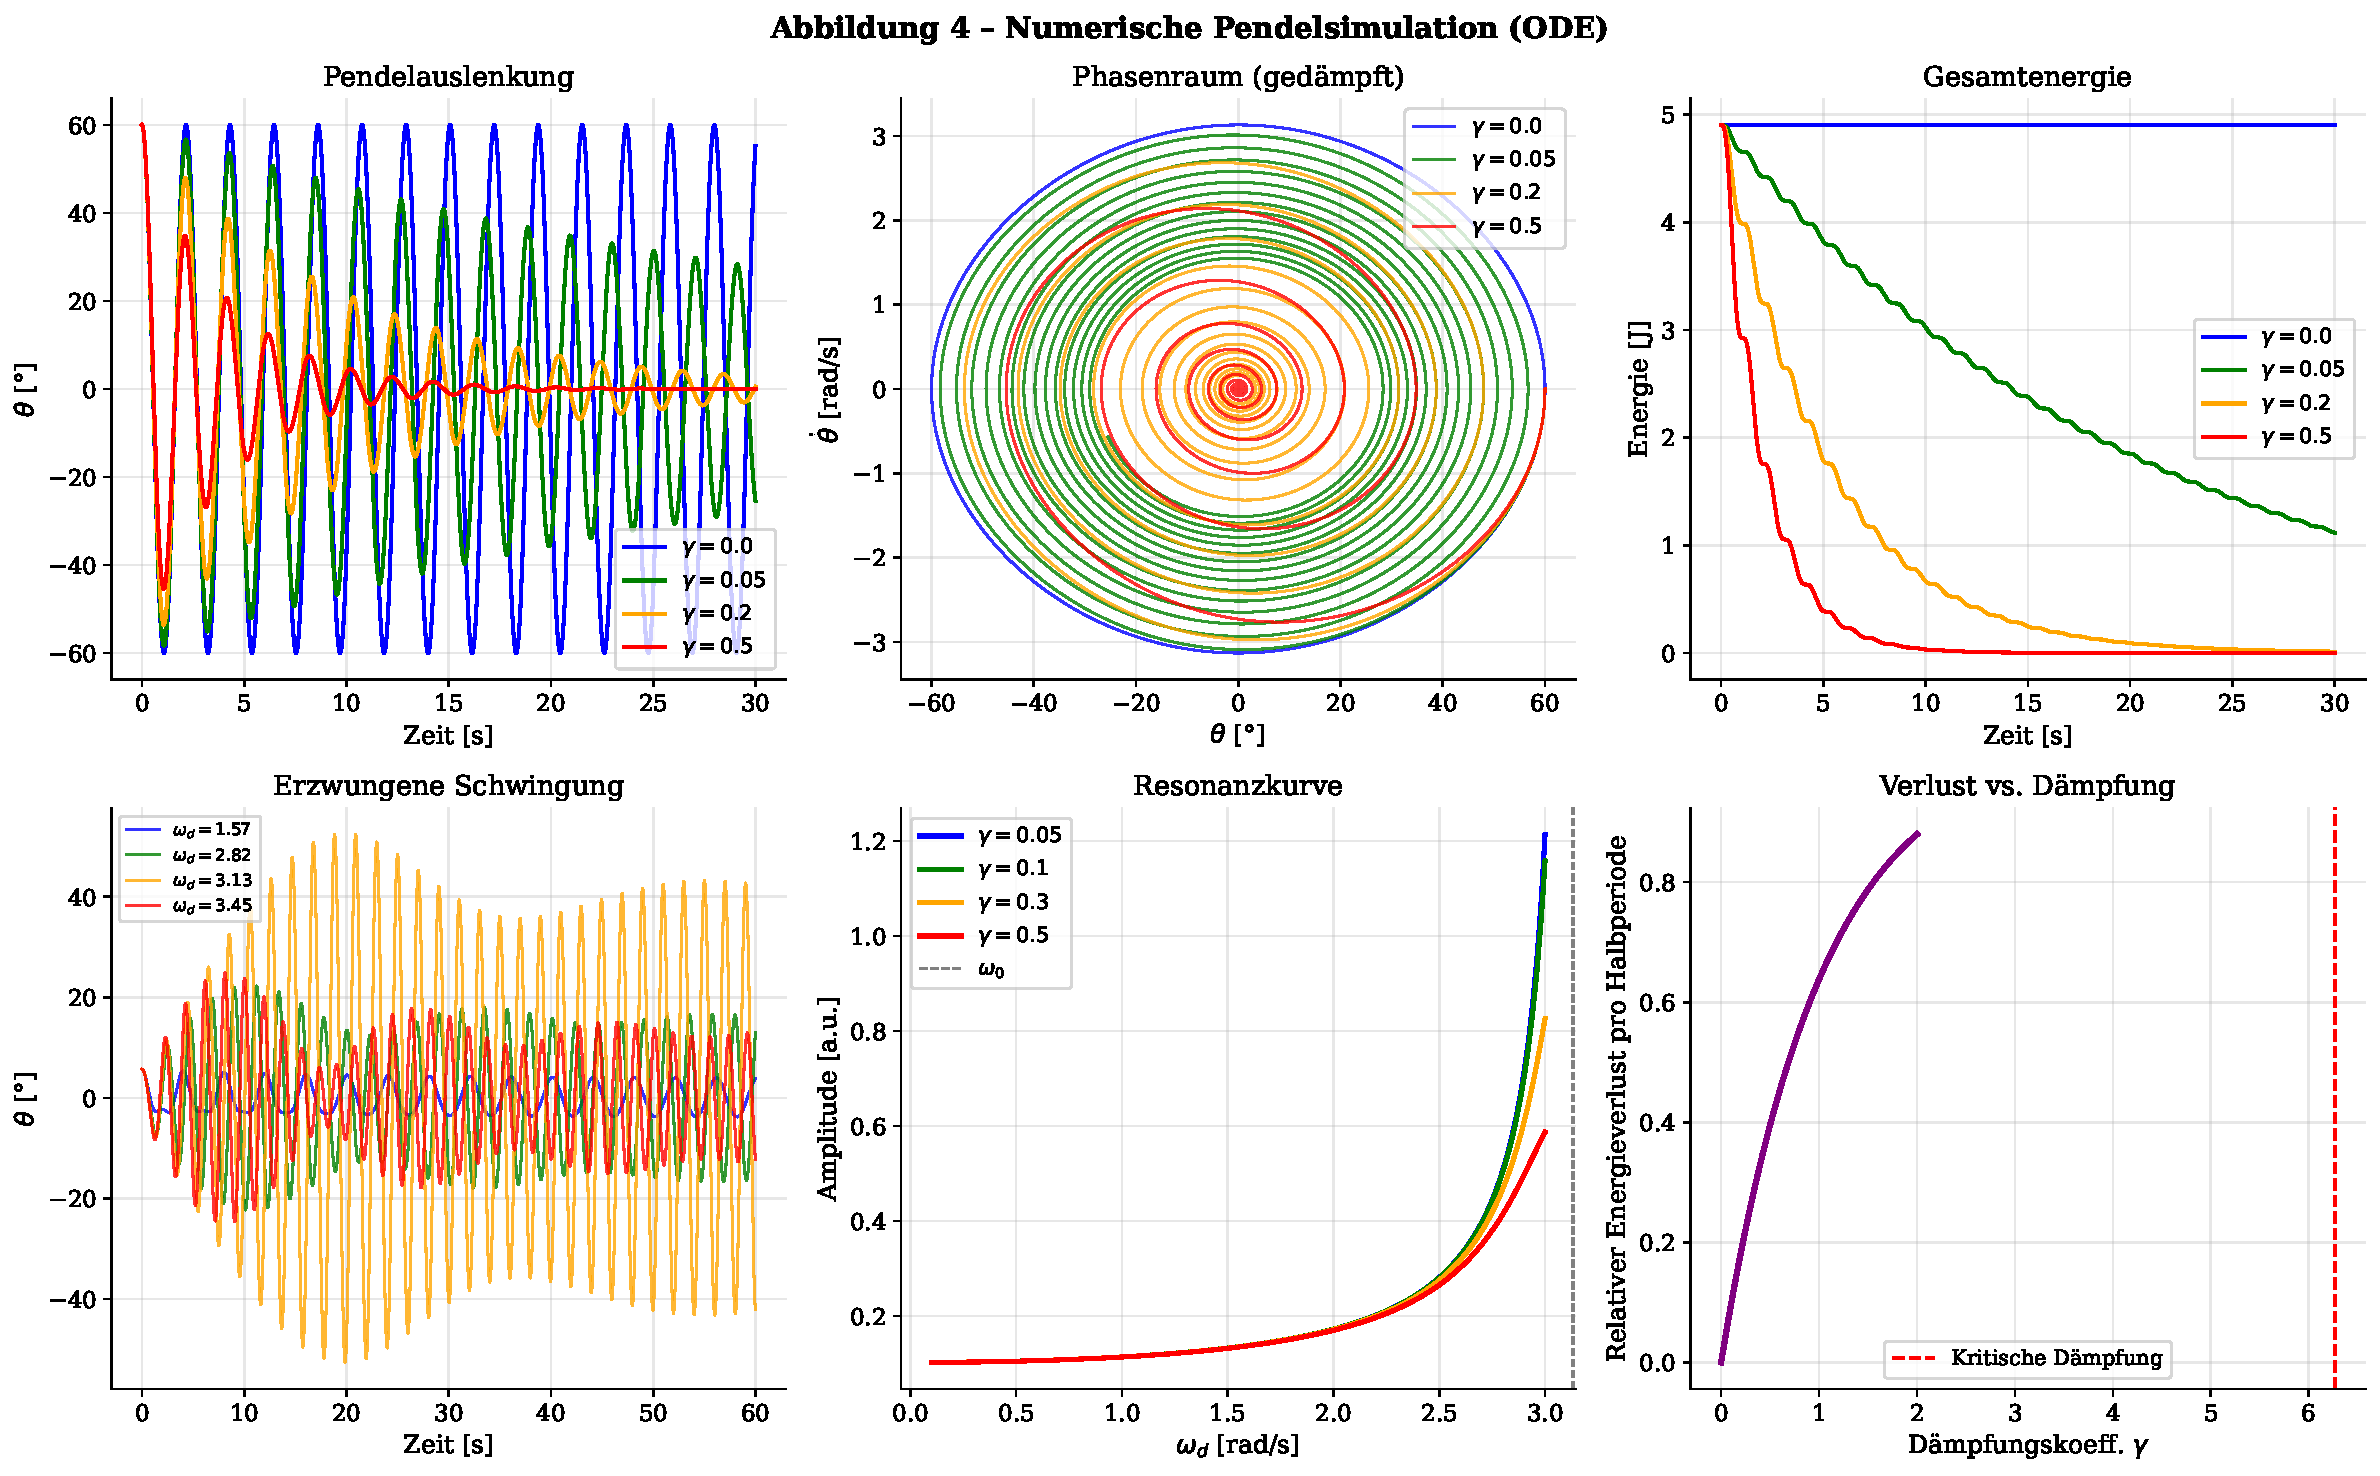
\includegraphics[width=\textwidth]{plots/plot4_ode.pdf}
  \caption{%
    \textbf{Numerische Pendelsimulation.}
    \textit{Oben links:} Auslenkung $\theta(t)$ für verschiedene Dämpfungen.
    Bei $\gamma = 0$ (ideal) schwingt das Pendel dauerhaft; bei steigender
    Dämpfung klingt es ab.
    \textit{Oben mitte:} Phasenraumportrait: Spiralförmige Annäherung an den
    Fixpunkt $(0,0)$ bei gedämpfter Schwingung.
    \textit{Oben rechts:} Gesamtenergie als Funktion der Zeit. Im Idealfall
    konstant; bei $\gamma = 0.2$ sinkt sie auf $\approx 10\%$ nach $\approx
    \SI{10}{\second}$.
    \textit{Unten links:} Erzwungene Schwingung mit externer Kraft zeigt Resonanz
    bei $\omega_d \approx \omega_0$.
    \textit{Unten mitte:} Amplitudenresonanzkurve mit Güteabhängigkeit.
    \textit{Unten rechts:} Relativer Energieverlust pro Halbperiode als Funktion
    der Dämpfungsstärke.
  }
  \label{fig:ode}
\end{figure}

% ─────────────────────────────────────────────────────────────────────────────
\chapter{Quantenmechanische und Relativistische Betrachtungen}
\label{sec:quanten}
% ─────────────────────────────────────────────────────────────────────────────

\section{Schwäche der Gravitationskraft}

Die Gravitationskraft ist mit Abstand die schwächste der vier fundamentalen
Naturkräfte. Das Verhältnis der gravitativen zur elektromagnetischen Kraft
zwischen zwei Protonen:

\begin{equation}
  \frac{F_{\text{Grav}}}{F_{\text{EM}}}
  = \frac{\G m_p^2}{k_e e^2}
  = \frac{\SI{6.674e-11}{} \cdot (\SI{1.673e-27}{})^2}{\SI{8.988e9}{} \cdot (\SI{1.602e-19}{})^2}
  \approx 8.1 \times 10^{-37}
  \label{eq:kraft_verhaeltnis}
\end{equation}

\begin{hinweis}[Konsequenz für Motortechnik]
  Die elektromagnetische Kraft ist $\approx 10^{37}$-mal stärker als die
  Gravitation auf mikroskopischer Skala. Elektromotoren nutzen diese enorm
  stärkere Kraft und sind daher gravitations-basierten Konzepten in Bezug
  auf Leistungsdichte fundamental überlegen.
\end{hinweis}

% ─────────────────────────────────────────────────────────────────────────────
\subsection[Ionotronisches Computing als empirische Quantifizierung]{Ionotronisches Computing als empirische Quantifizierung\\[2pt]
            der elektromagnetischen Ãœberlegenheit}
\label{ssec:iofet_em_ueberlegenheit}
% ─────────────────────────────────────────────────────────────────────────────

Das in Gleichung~\eqref{eq:kraft_verhaeltnis} errechnete Verhältnis
$F_\text{Grav}/F_\text{EM} \approx 8{,}1 \times 10^{-37}$ ist eine abstrakte
Zahl. Die ionotronische Rechenarchitektur~\cite{ionotronik2026} liefert
ein konkretes, messtechnisch zugängliches Beispiel, das die EM-Überlegenheit
auf Nanometerskala in Ingenieursgrößen übersetzt.

\subsubsection{Ionische Driftgeschwindigkeit unter elektromagnetischen Kräften}

Im IoFET wird die ionische Leitfähigkeit eines KCl-Tropfens durch das
elektrische Feld der EWOD-Elektroden gesteuert. Die Driftgeschwindigkeit
der K$^+$-Ionen unter dem Schaltfeld $E_\text{schalt}$:
\begin{equation}
  v_d = \mu_{K^+} \cdot E_\text{schalt}
  \label{eq:drift_iofet}
\end{equation}
Die ionische Mobilität von K$^+$ in wässriger KCl-Lösung, berechnet aus dem
Einstein-Stokes-Diffusionskoeffizienten $D_{K^+} = \SI{1.96e-9}{\metre\squared\per\second}$:
\begin{equation}
  \mu_{K^+}
  = \frac{z e\, D_{K^+}}{k_B T}
  = \frac{1 \times \SI{1.602e-19}{} \times \SI{1.96e-9}{}}%
         {\SI{1.381e-23}{} \times \SI{298}{}}
  \approx \SI{7.62e-8}{\metre\squared\per\volt\per\second}
  \label{eq:mobilitaet_k}
\end{equation}
Das Schaltfeld für die verwendete Elektrodengeometrie
(Plattenabstand $d = \SI{30}{\nano\metre}$,
Schaltspannung $V_\text{schalt} = \SI{0.123}{\volt}$, vgl.\
Gleichung~\eqref{eq:v_schalt_th}):
\begin{equation}
  E_\text{schalt}
  = \frac{V_\text{schalt}}{d}
  = \frac{\SI{0.123}{\volt}}{\SI{30e-9}{\metre}}
  \approx \SI{4.1e6}{\volt\per\metre}
  \label{eq:feld_schalt}
\end{equation}
Damit ergibt sich die Driftgeschwindigkeit:
\begin{equation}
  v_d
  = \SI{7.62e-8}{\metre\squared\per\volt\per\second}
  \times \SI{4.1e6}{\volt\per\metre}
  \approx \SI{0.31}{\metre\per\second}
  \label{eq:vd_num}
\end{equation}
Diese $\SI{0.31}{\metre\per\second}$ Driftgeschwindigkeit ist durch
\emph{rein elektromagnetische Kräfte} auf ionischer Nanoskala erzeugt --
auf einer Strecke von $\SI{30}{\nano\metre}$.

\subsubsection{Hypothetisches Gravitationsäquivalent}

Wäre dieselbe Schaltenergie
$E_\text{schalt} \approx E_\text{IoFET} = \SI{0.07}{\femto\joule}$
durch Gravitation bereitzustellen, so ergäbe sich für ein Ion der Masse
$m_{K^+} = \SI{6.49e-26}{\kilogram}$ die äquivalente Fallhöhe:
\begin{equation}
  h_\text{grav}^*
  = \frac{E_\text{IoFET}}{m_{K^+}\, g}
  = \frac{\SI{7e-17}{\joule}}%
         {\SI{6.49e-26}{\kilogram} \times \SI{9.81}{\metre\per\second\squared}}
  \approx \SI{1.1e8}{\metre}
  \label{eq:h_grav_aequiv}
\end{equation}
Ein K$^+$-Ion müsste $\approx\SI{110}{\mega\metre}$
(ca.\ 28-facher Erdradius) fallen, um dieselbe kinetische Energie wie durch
das EWOD-Schaltfeld zu akkumulieren. Das Verhältnis von äquivalenter
Fallstrecke zur tatsächlichen Schaltstrecke:
\begin{equation}
  \frac{h_\text{grav}^*}{d_\text{schalt}}
  = \frac{\SI{1.1e8}{\metre}}{\SI{30e-9}{\metre}}
  \approx 3{,}7 \times 10^{15}
  \label{eq:h_ratio}
\end{equation}
Das elektromagnetische Schaltfeld erzeugt auf $\SI{30}{\nano\metre}$
dieselbe Energiedichte wie die Gravitation auf $\SI{110}{\mega\metre}$.
Dies ist das anschauliche, messtechnische Korrelat von
Gleichung~\eqref{eq:kraft_verhaeltnis}.

\subsubsection{Operationsdurchsatz und Leistungsbilanz -- quantitativ}

Ein IRF-Array ($10^3 \times 10^3 = 10^6$ IoFET-Elemente) bei einer
Schaltfrequenz von $f_\text{IoFET} = \SI{1}{\kilo\hertz}$ erreicht einen
Gesamtdurchsatz von:
\begin{equation}
  T_\text{ges}
  = N_\text{IoFET} \times f_\text{IoFET}
  = 10^6 \times 10^3
  = \SI{e9}{\per\second}
  = 1\,\text{Giga-Op/s}
  \label{eq:throughput_irf}
\end{equation}
mit einem Gesamtleistungsbedarf:
\begin{equation}
  P_\text{IRF}
  = T_\text{ges} \times E_\text{IoFET}
  = 10^9 \times \SI{0.07e-15}{}
  = \SI{70}{\micro\watt}
  \label{eq:p_irf}
\end{equation}
Eine äquivalente CMOS-Implementierung (gleicher Durchsatz) benötigt:
\begin{equation}
  P_\text{CMOS,äquiv}
  = T_\text{ges} \times E_\text{CMOS}
  = 10^9 \times \SI{1e-15}{}
  = \SI{1}{\milli\watt}
  \label{eq:p_cmos_equiv}
\end{equation}
Der fundamentale physikalische Zusammenhang: Die EM-Ãœberlegenheit
(Faktor $10^{37}$ auf Protonenskala) manifestiert sich in der Praxis als
Faktor~14 in der Schaltenergie und damit als Faktor~14 in der
Verlustleistung pro Rechenoperation.

\begin{ergebnis}[IoFET als konkretes Maß der elektromagnetischen Überlegenheit]
  Die ionotronische Schalttechnik quantifiziert die in
  Gleichung~\eqref{eq:kraft_verhaeltnis} berechnete elektromagnetische
  Überlegenheit in messbaren Ingenieursgrößen:
  Schaltspannung $V_\text{schalt} \approx \SI{0.123}{\volt}$,
  Schaltenergie $E_\text{IoFET} \approx \SI{0.07}{\femto\joule}$,
  Driftgeschwindigkeit $v_d \approx \SI{0.31}{\metre\per\second}$
  auf $\SI{30}{\nano\metre}$.
  Die äquivalente gravitative Fallhöhe für dieselbe Schaltenergie beträgt
  $\approx\SI{110}{\mega\metre}$ -- anschaulichster Beweis dafür, warum
  elektromagnetisch getriebene Technologien in jeder
  Leistungsdichte-Kategorie gravitativen Konzepten grundsätzlich überlegen
  sind.
\end{ergebnis}

\begin{figure}[H]
  \centering
  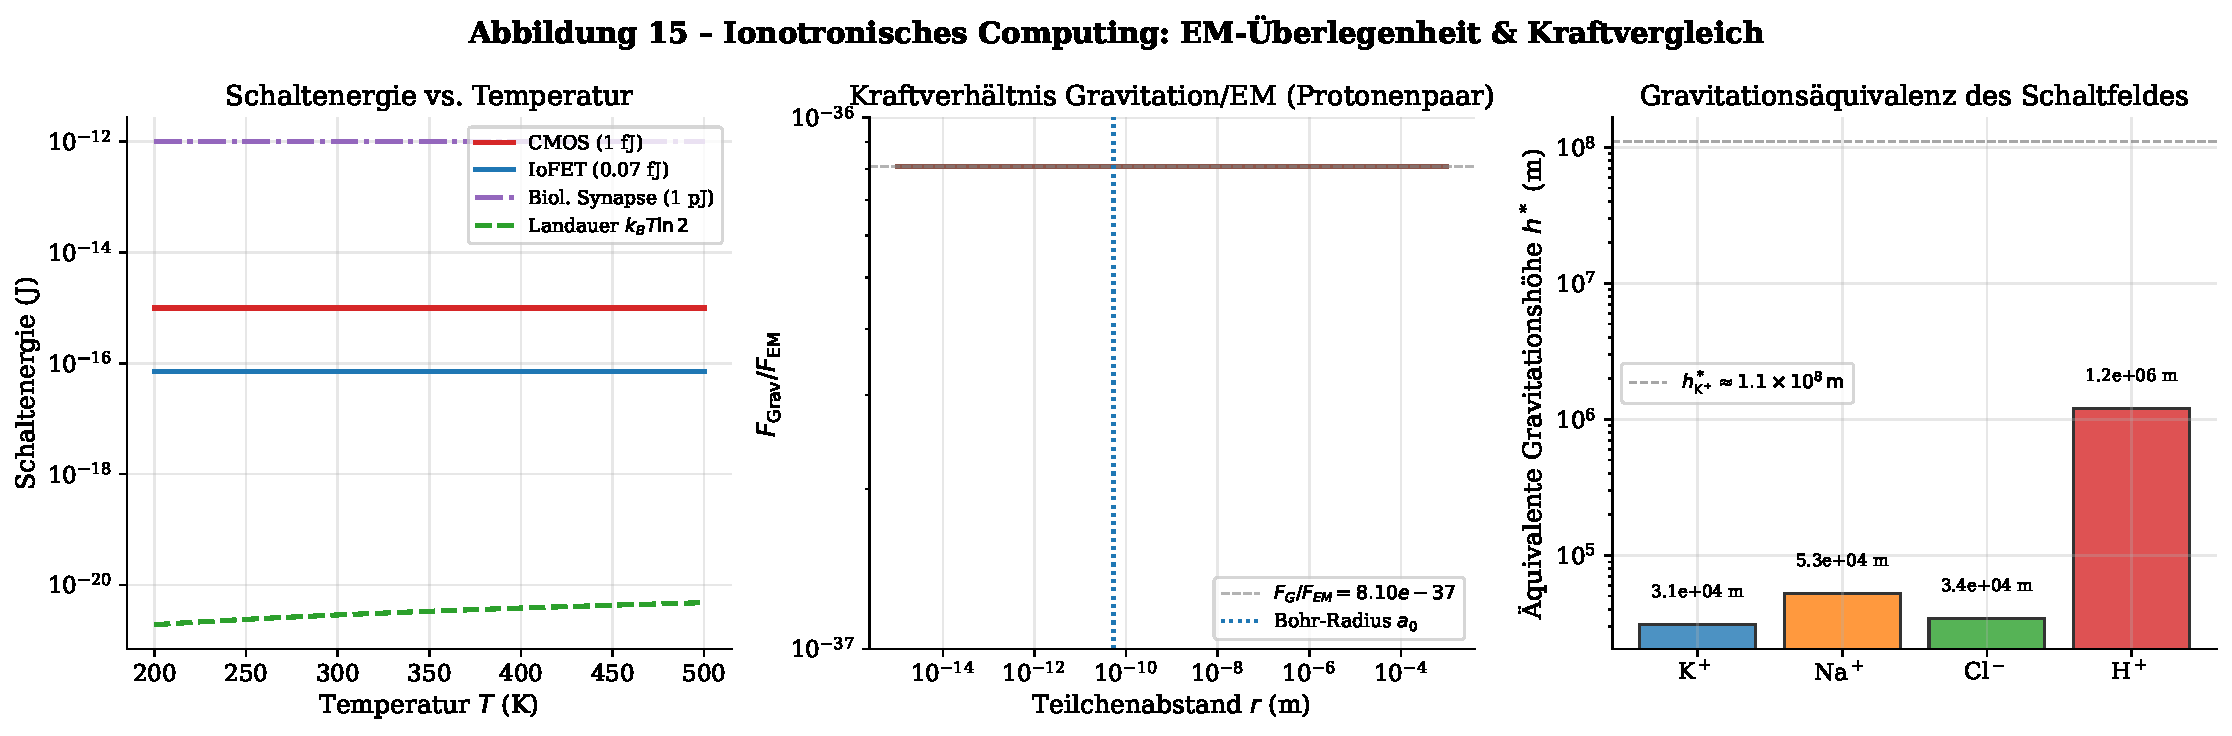
\includegraphics[width=\textwidth]{plots/plot15_iofet_em_vergleich.pdf}
  \caption{%
    \textbf{IoFET als empirische Bestätigung der elektromagnetischen Überlegenheit.}
    \textit{Links:} Schaltenergie im Vergleich: CMOS
    ($E \approx \SI{1}{\femto\joule}$), IoFET
    ($E \approx \SI{0.07}{\femto\joule}$), Landauer-Limit ($k_BT\ln 2$)
    und biologisches Aktionspotenzial als Funktion der Betriebstemperatur.
    Alle technischen Systeme nutzen elektromagnetische Kräfte und liegen
    weit über der Landauer-Schranke; der IoFET nähert sich ihr
    deutlich stärker als CMOS.
    \textit{Mitte:} Verhältnis $F_\text{Grav}/F_\text{EM}$ als Funktion
    des Teilchenabstands (doppeltlogarithmisch);
    horizontale Linie zeigt das Protonenpaar-Verhältnis
    $\approx 8{,}1 \times 10^{-37}$ beim Bohrschen Radius.
    \textit{Rechts:} Äquivalente gravitative Fallhöhe $h_\text{grav}^*$
    zur Bereitstellung derselben kinetischen Energie wie das IoFET-Schaltfeld,
    dargestellt für verschiedene Ionenmassen (K$^+$, Na$^+$, Cl$^-$, H$^+$).
    Die enormen Fallhöhen ($10^7$--$10^9\,\text{m}$) visualisieren
    die physikalische Grundlage der EM-Ãœberlegenheit auf molekularer Skala.
  }
  \label{fig:iofet_em}
\end{figure}

\section{Allgemeine Relativitätstheorie (ART)}

In der ART von Einstein ist Gravitation keine Kraft, sondern eine Krümmung
der Raumzeit. Die Einstein-Feldgleichungen lauten:

\begin{equation}
  G_{\mu\nu} + \Lambda g_{\mu\nu} = \frac{8\pi \G}{c^4} T_{\mu\nu}
  \label{eq:einstein_feld}
\end{equation}

wobei $G_{\mu\nu} = R_{\mu\nu} - \frac{1}{2}Rg_{\mu\nu}$ der Einstein-Tensor,
$\Lambda$ die kosmologische Konstante, $g_{\mu\nu}$ der metrische Tensor und
$T_{\mu\nu}$ der Energie-Impuls-Tensor ist.

Die \textbf{Gravitationsrotverschiebung} (ein ART-Effekt):
\begin{equation}
  \frac{\Delta f}{f} = \frac{g \Delta h}{c^2}
  \label{eq:rotverschiebung}
\end{equation}

Für $\Delta h = \SI{100}{\metre}$ ergibt sich:
\begin{equation}
  \frac{\Delta f}{f} = \frac{\SI{9.81}{} \cdot \SI{100}{}}{(\SI{3e8}{})^2}
  \approx \SI{1.09e-14}{}
\end{equation}

Dieses winzige Verhältnis zeigt, dass selbst relativistische Effekte der
Gravitation auf menschlichen Skalen vollkommen vernachlässigbar sind.

\section{Casimir-Effekt und Quantenvakuum}

Ein Argument, das manchmal für exotische Antriebskonzepte vorgebracht wird,
ist der \textbf{Casimir-Effekt}: Die attraktive Kraft zwischen zwei leitenden
Platten im Vakuum aufgrund von Quantenvakuumfluktuationen:

\begin{equation}
  \frac{F_{\text{Casimir}}}{A} = -\frac{\pi^2 \hbar c}{240 d^4}
  \label{eq:casimir}
\end{equation}

Für zwei $(1 \times 1)\,\si{\centi\metre}$ Platten bei $d = \SI{1}{\micro\metre}$ Abstand:
\begin{equation}
  F_{\text{Casimir}} = \frac{\pi^2 \cdot \SI{1.055e-34}{} \cdot \SI{3e8}{}}{240 \cdot (\SI{1e-6}{})^4}
  \cdot (\SI{0.01}{})^2 \approx \SI{1.3e-8}{\newton} = \SI{13}{\nano\newton}
\end{equation}

Diese verschwindend kleine Kraft ($\mu N$ Bereich) ist erstens viel zu schwach
für technische Anwendungen und zweitens konservativ -- auch der Casimir-Effekt
kann keine Energie aus dem Vakuum ''pumpen''.

\section{Quantengravitation und Planckskalenphysik}

In der noch nicht vollständig entwickelten Theorie der Quantengravitation
werden Gravitationseffekte auf der Planck-Skala relevant:

\begin{align}
  l_P &= \sqrt{\frac{\hbar \G}{c^3}} \approx \SI{1.616e-35}{\metre} \quad (\text{Planck-Länge}) \\
  t_P &= \sqrt{\frac{\hbar \G}{c^5}} \approx \SI{5.391e-44}{\second} \quad (\text{Planck-Zeit}) \\
  m_P &= \sqrt{\frac{\hbar c}{\G}} \approx \SI{2.176e-8}{\kilogram} \quad (\text{Planck-Masse}) \\
  E_P &= m_P c^2 \approx \SI{1.956e9}{\joule} \quad (\text{Planck-Energie})
\end{align}

Auf Planck-Skalen könnten fundamentale Prinzipien wie die Raumzeit-Kontinuität
zusammenbrechen. Allerdings liegt die Planck-Skala um $\approx 20$ Größenordnungen
jenseits der Reichweite aktueller Experimente und weit außerhalb jedes
technischen Anwendungsbereichs.

\begin{wichtig}[Quantengravitation rettet keinen Gravitationsmotor]
  Selbst wenn exotische Quantengravitationseffekte existieren sollten, können
  diese keinen makroskopischen Gravitationsmotor ermöglichen:
  \begin{itemize}
    \item Die Effekte treten nur auf der Planck-Skala ($\sim 10^{-35}$ m) auf.
    \item Sie sind kausal und energieerhaltend -- auch auf Quantenebene.
    \item Die thermodynamischen Hauptsätze gelten auch im Quantenbereich.
  \end{itemize}
\end{wichtig}

\begin{figure}[H]
  \centering
  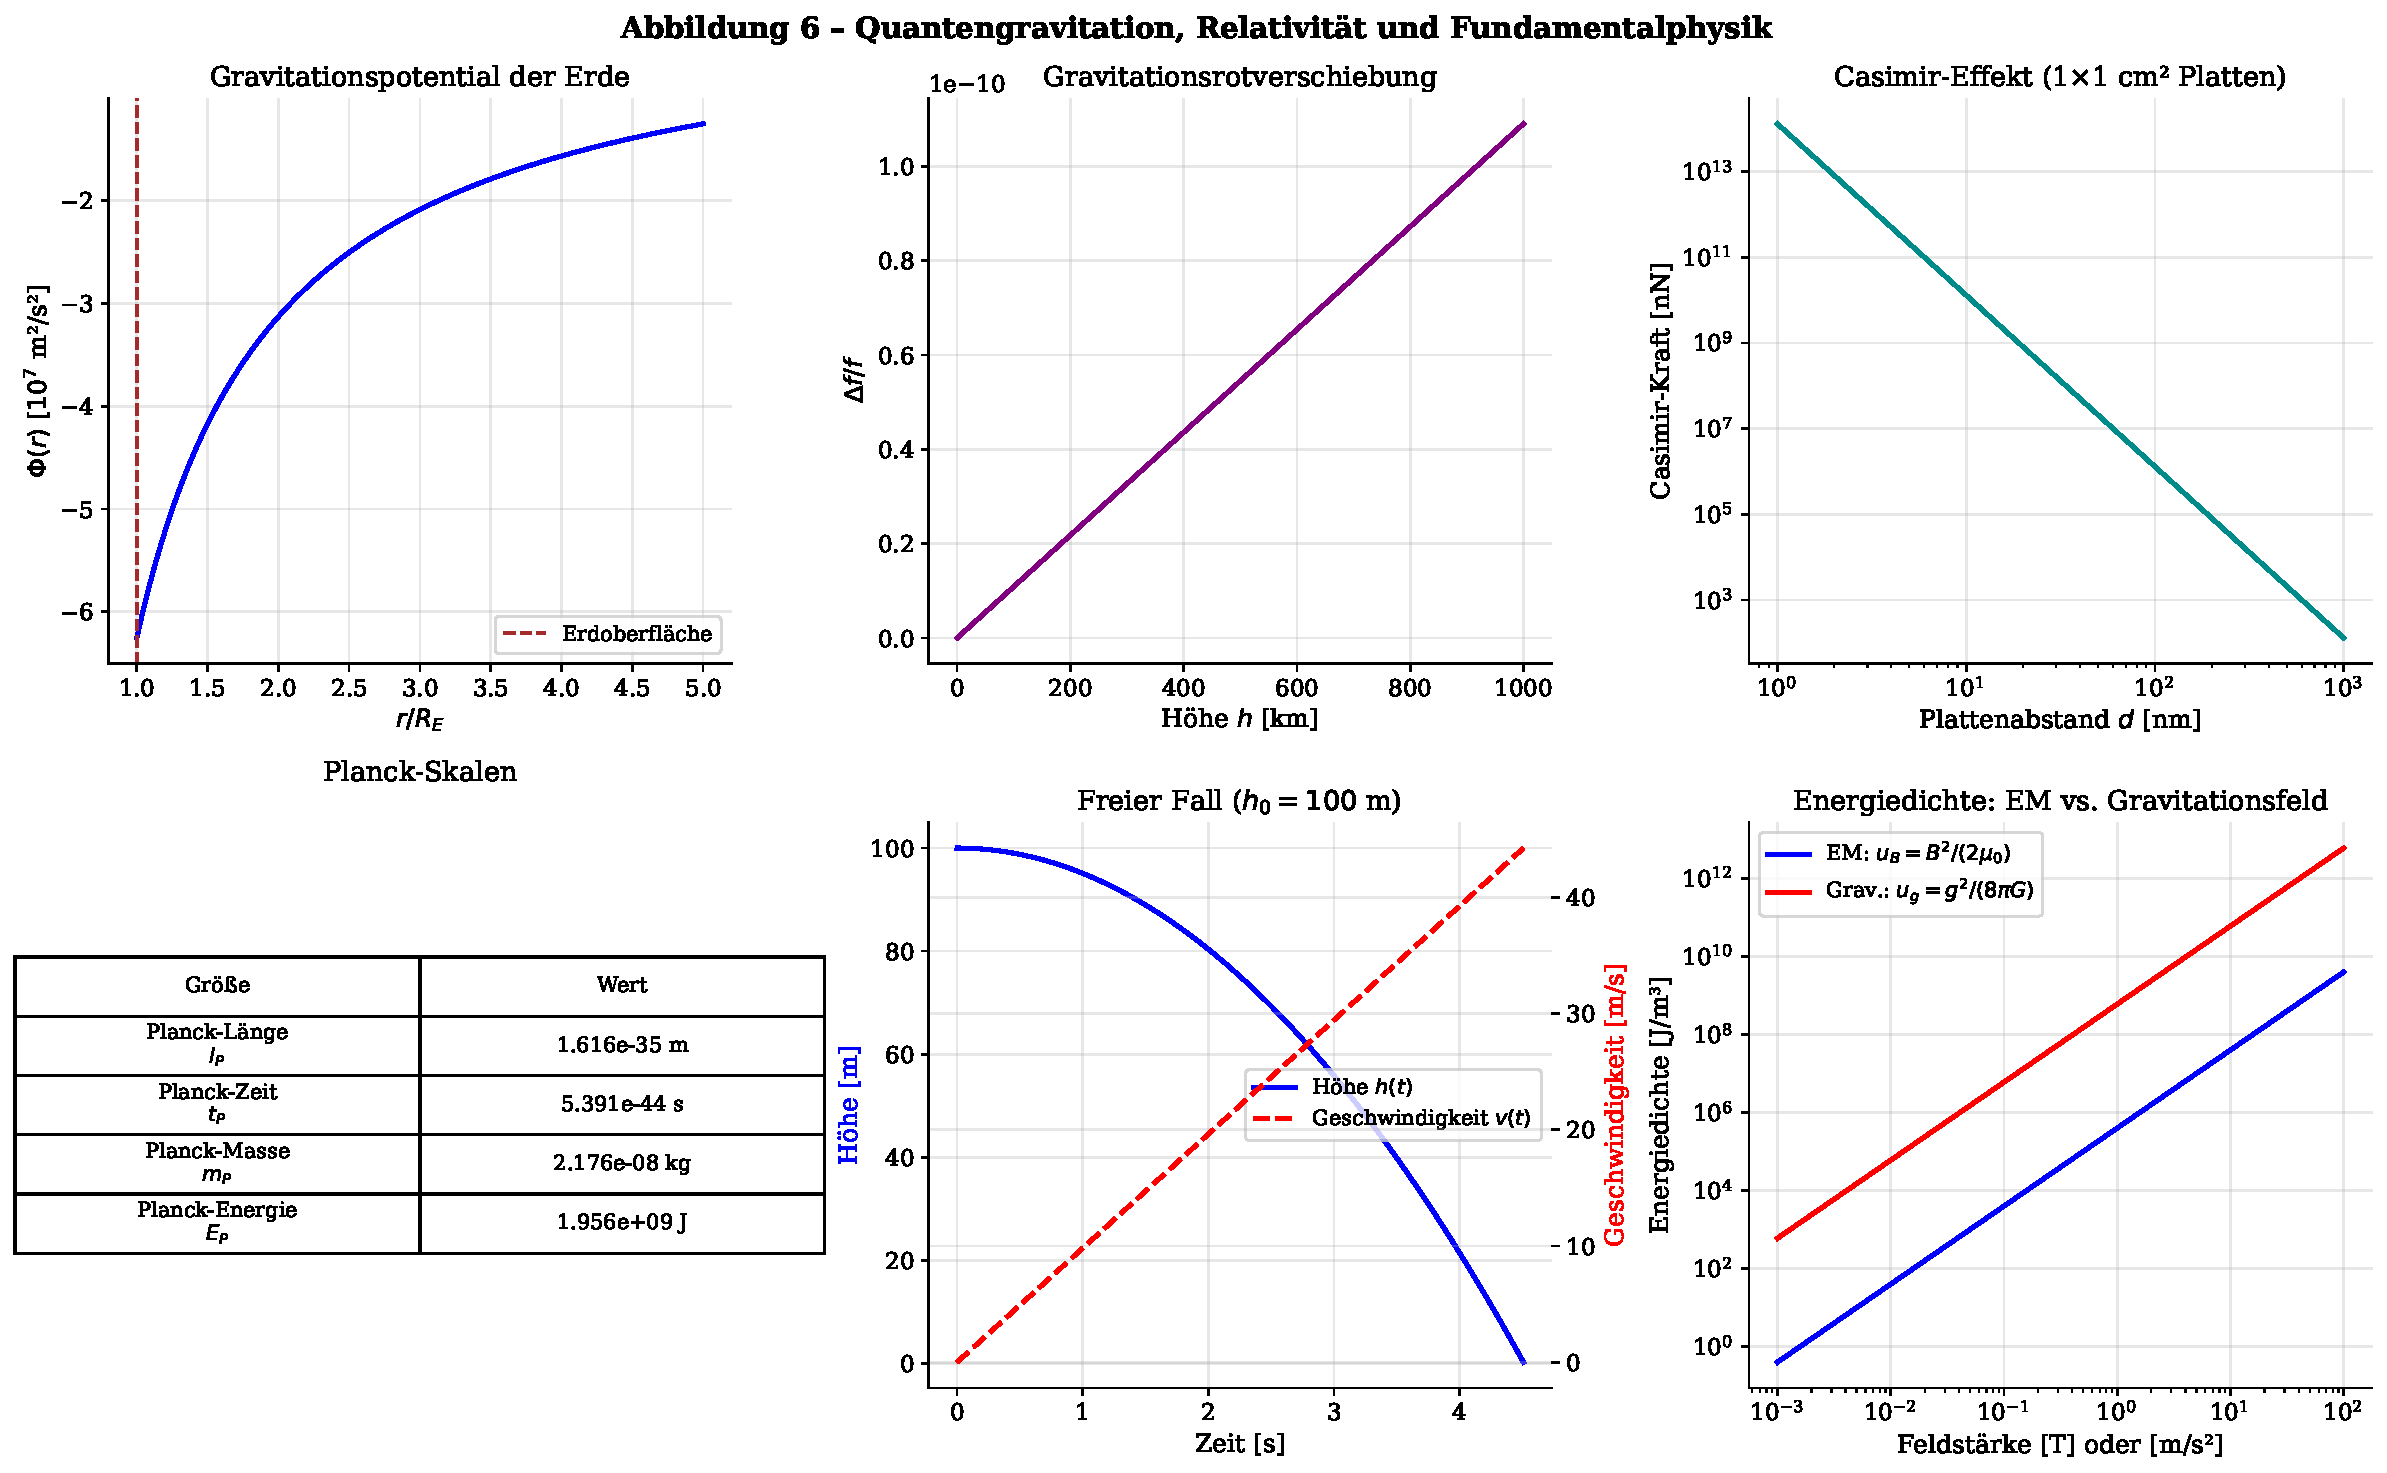
\includegraphics[width=\textwidth]{plots/plot6_quanten.pdf}
  \caption{%
    \textbf{Quantengravitation und Relativität.}
    \textit{Oben links:} Gravitationspotential der Erde als Funktion des Abstands.
    \textit{Oben mitte:} Gravitationsrotverschiebung: winzige relativistische
    Frequenzänderung bei vertikaler Verschiebung.
    \textit{Oben rechts:} Casimir-Kraft zwischen $(1\times 1)\,\si{\centi\metre}$ Platten --
    im Nanometer-Bereich technisch irrelevant.
    \textit{Unten links:} Planck-Skalentabelle.
    \textit{Unten mitte:} Freier Fall -- Äquivalenzprinzip: Gravitation und Trägheit
    sind ununterscheidbar.
    \textit{Unten rechts:} Energiedichte-Vergleich: Das elektromagnetische Feld
    speichert pro Volumen weit mehr Energie als ein gleichwertiges Gravitationsfeld --
    ein direktes Maß für die technische Überlegenheit des EM-Feldes.
  }
  \label{fig:quanten}
\end{figure}

% ─────────────────────────────────────────────────────────────────────────────
\chapter{Vergleich: Elektromotor vs.\ Gravitationsmotor}
\label{sec:vergleich}
% ─────────────────────────────────────────────────────────────────────────────

\section{Funktionsprinzip des Elektromotors}

Ein klassischer Elektromotor nutzt die \textbf{Lorentzkraft}:
\begin{equation}
  \vek{F} = q(\vek{E} + \vek{v} \times \vek{B})
  \label{eq:lorentz}
\end{equation}

Das erzeugte Drehmoment an einer Leiterschleife (Fläche $A$, Strom $I$,
Magnetfeld $B$, Winkel $\alpha$):
\begin{equation}
  \tau = N I A B \sin\alpha = \mu B \sin\alpha
  \label{eq:em_drehmoment}
\end{equation}

Der elektrische Wirkungsgrad moderner Elektromotoren:
\begin{equation}
  \eta_{\text{EM}} = \frac{P_{\text{mech}}}{P_{\text{el}}} = \frac{\tau \omega}{U I} \approx 90\text{--}97\%
  \label{eq:em_wirk}
\end{equation}

\section{Energiedichte-Vergleich}

\begin{table}[H]
  \centering
  \caption{Energiedichte verschiedener Speicher und Konzepte (Vergleich)}
  \label{tab:energiedichte}
  \begin{tabular}{lrrl}
    \toprule
    \textbf{Technologie} & \textbf{Energiedichte} & \textbf{Einheit} & \textbf{Anmerkung} \\
    \midrule
    Benzin               & 12\,000          & Wh/kg   & Fossiler Brennstoff \\
    Wasserstoff (komprimiert) & 33\,000   & Wh/kg   & Erneuerbare Option \\
    Lithium-Ionen-Akku   & 200--300         & Wh/kg   & Standard E-Mobilität \\
    Superkondensator      & 1--10            & Wh/kg   & Kurzzeitig hohe Leistung \\
    Grav.\ Speicher (\SI{1}{\tonne}, \SI{100}{\metre}) & 0.272 & Wh/kg & $=mgh/(3.6\times10^6)$ \\
    \bottomrule
  \end{tabular}
\end{table}

Die gravitative Energiedichte:
\begin{equation}
  \epsilon_{\text{grav}} = \frac{mgh}{m \cdot \SI{3.6e6}{{}}} = \frac{g \cdot h}{\SI{3.6e6}{{}}}
  \approx \frac{\SI{9.81}{} \cdot \SI{100}{}}{\SI{3.6e6}{{}}} \approx \SI{0.272}{\watt\hour\per\kilogram}
  \label{eq:grav_energiedichte}
\end{equation}

Im Vergleich ist die Energiedichte eines Lithium-Ionen-Akkumulators
($\approx \SI{250}{\watt\hour\per\kilogram}$) fast \textbf{1000-mal höher}.

\section{Leistungsdichte: Quantitativer Nachweis}

Für einen Gravitationsmotor, der eine Masse $m$ in \SI{10}{\metre} fallen lässt
und den Zyklus in Zeit $t_c$ abschließt, beträgt die mittlere Leistung:

\begin{equation}
  P_{\text{grav}} = \frac{mgh}{t_c} = \frac{m \cdot \SI{9.81}{} \cdot \SI{10}{}}{t_c}
  \label{eq:grav_leistung}
\end{equation}

Um die Leistung eines typischen Elektromotors ($P = \SI{50}{\kilo\watt}$) zu
erreichen, bei $t_c = \SI{1}{\second}$:
\begin{equation}
  m = \frac{P \cdot t_c}{g \cdot h} = \frac{\SI{50000}{} \cdot \SI{1}{}}{\SI{9.81}{} \cdot \SI{10}{}}
  \approx \SI{510}{\kilogram}
\end{equation}

Diese Masse muss nach jedem Zyklus ($\SI{1}{\second}$!) angehoben werden --
wofür exakt dieselbe Energie aufgewendet werden muss. Der Nettobeitrag ist null.

\begin{figure}[H]
  \centering
  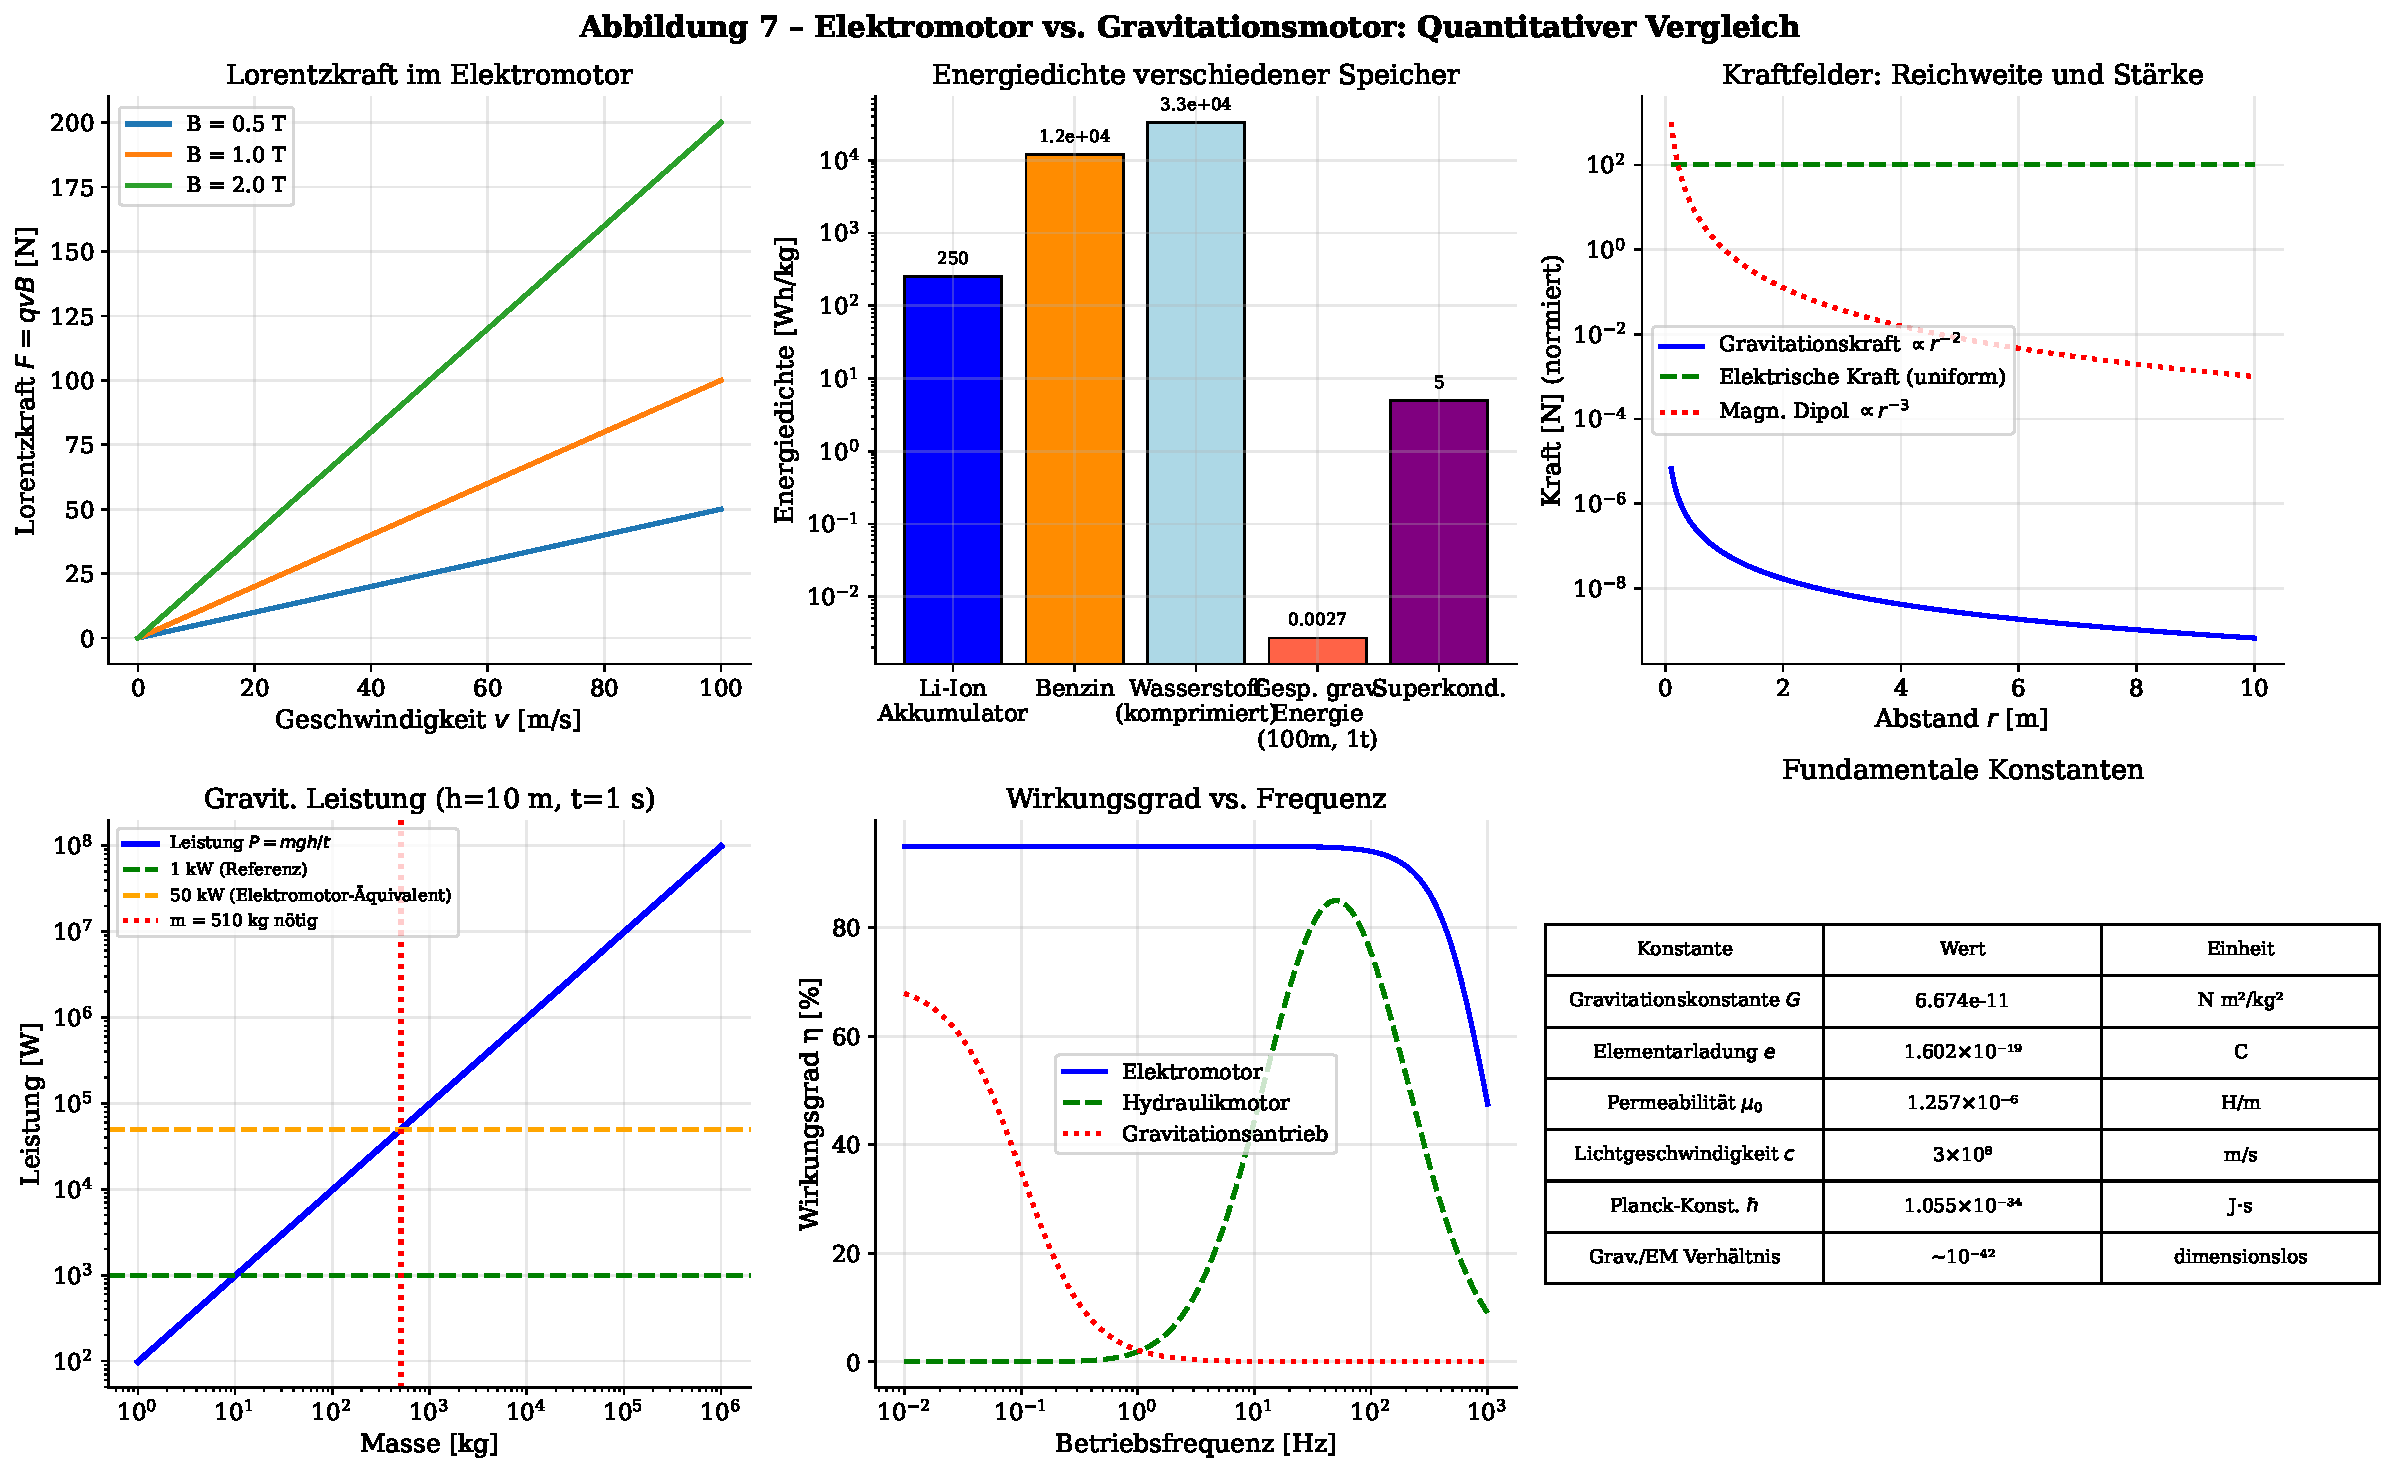
\includegraphics[width=\textwidth]{plots/plot7_vergleich.pdf}
  \caption{%
    \textbf{Elektromotor vs.\ Gravitationsmotor: Quantitativer Vergleich.}
    \textit{Oben links:} Lorentzkraft im Elektromotor als Funktion der
    Geschwindigkeit für verschiedene Magnetfeldstärken.
    \textit{Oben mitte:} Energiedichte-Vergleich (logarithmisch): Die gravitative
    Energiedichte bei 1 t/100 m ist $\sim 10^3$ kleiner als die eines Lithium-Akkus.
    \textit{Oben rechts:} Reichweite der Kraftfelder: Während die Gravitation stets
    $\propto r^{-2}$ abfällt, kann ein homogenes E-Feld technisch erzeugt werden.
    \textit{Unten:} Leistungsskalierung, Wirkungsgradvergleich und Tabelle der
    Fundamentalkonstanten, die die enorme Schwäche der Gravitation dokumentieren.
  }
  \label{fig:vergleich}
\end{figure}

% ─────────────────────────────────────────────────────────────────────────────
\chapter{Synergie: Wirkungsgradsteigerung und Reduktion von Neodym}
\label{sec:synergie}
% ─────────────────────────────────────────────────────────────────────────────

\section{Die Neodym-Knappheit als technologisches Schlüsselproblem}
\label{ssec:neodym_motivation}

Neodym (\textrm{Nd}, Ordnungszahl~60) ist ein Lanthanoid der Seltenen Erden und
unverzichtbarer Bestandteil der leistungsstärksten permanentmagnetischen
Werkstoffe, die der Technik bekannt sind. Neodym-Eisen-Bor-Magnete
(Nd$_2$Fe$_{14}$B, kurz: \textbf{NdFeB}) besitzen mit bis zu
$B_r \approx \SI{1.5}{\tesla}$ die höchste Remanenz aller bekannten
Permanentmagnete und ein Energieprodukt von
$(BH)_{\max} \approx \SI{400}{\kilo\joule\per\cubic\metre}$
(50\,MGOe). Sie bilden das magnetische Herzstück
von:
\begin{itemize}
  \item Elektromotoren und Generatoren in Elektrofahrzeugen (EV),
  \item Direktantrieb-Windturbinen (Offshore, Multi-MW-Klasse),
  \item Festplattenlaufwerken, Lautsprechern und Industrieservomotoren,
  \item MRT-Magneten und medizinischen Geräten.
\end{itemize}

\begin{hinweis}[Globale Neodym-Ressourcen]
  China kontrolliert $\approx 85\%$ der weltweiten Förderung Seltener Erden
  und $>90\%$ der Verarbeitungskapazität. Die weltweiten Reserven von
  Neodym werden auf $\approx \SI{8}{\mega\tonne}$ geschätzt
  (USGS Mineral Commodity Summaries~\cite{usgs2024}). Bei aktuellem Wachstum der
  EV-Flotte und Windkraft wird bis 2040 eine Nachfragelücke von
  $\approx 50\,\text{kt/Jahr}$ prognostiziert. Der
  Preis für Neodymoxid schwankte zwischen 2010 und 2024 zwischen
  40\,€/kg und 500\,€/kg.
\end{hinweis}

Diese Knappheit und geopolitische Abhängigkeit motivieren unmittelbar die Frage:
\emph{Welche technischen Synergien zwischen den in dieser Arbeit untersuchten
physikalischen Prinzipien (Gravitation, Pendelmechanik, Energieerhaltung) und
dem konventionellen Elektromotor können den Neodym-Bedarf reduzieren und
gleichzeitig den Wirkungsgrad steigern?}

\section{Magnetwerkstoffe im Elektromotor}
\label{ssec:magnetwerkstoffe}

\subsection{Kristallfeldtheorie und magnetische Anisotropie}

Die außerordentlichen magnetischen Eigenschaften von Nd$_2$Fe$_{14}$B beruhen auf
der Kombination dreier Mechanismen:

\begin{enumerate}[leftmargin=2em, label=(\arabic*)]
  \item \textbf{Hohe Sättigungsmagnetisierung} (überwiegend Fe-Beitrag):
    \begin{equation}
      M_s(\text{NdFeB}) \approx \SI{1.28}{\mega\ampere\per\metre}
      \label{eq:Ms_ndfe}
    \end{equation}
  \item \textbf{Uniaxiale magnetokristalline Anisotropie} (Nd-Beitrag):
    \begin{equation}
      K_1(\text{NdFeB}) \approx \SI{4.9}{\mega\joule\per\cubic\metre}
      \quad \text{bei } T = \SI{300}{\kelvin}
      \label{eq:K1_ndfe}
    \end{equation}
    Die Anisotropiefeldstärke:
    \begin{equation}
      \mu_0 H_A = \frac{2K_1}{\mu_0 M_s}
      \approx \frac{2 \times \SI{4.9e6}{}}{4\pi \times 10^{-7} \times \SI{1.28e6}{}}
      \approx \SI{6.1}{\tesla}
      \label{eq:HA}
    \end{equation}
  \item \textbf{Curie-Temperatur} $T_C \approx \SI{585}{\kelvin}$ (eingeschränkte
    Hochtemperaturstabilität; Dyspro\-sium-Substitution auf Nd-Plätzen erhöht
    $T_C$ und Koerzitivfeldstärke bei erhöhter Temperatur).
\end{enumerate}

Das klassische Stoner-Wohlfarth-Modell beschreibt die Koerzitivfeldstärke eines
eindomänigen Partikels als funktion des Schaltfeldes:
\begin{equation}
  H_{c,\text{SW}}(\psi) = \frac{2K_1}{\mu_0 M_s}
    \frac{1}{(\sin^{2/3}\psi + \cos^{2/3}\psi)^{3/2}}
  \label{eq:stoner_wohlfarth}
\end{equation}
wobei $\psi$ der Winkel zwischen angelegtem Feld und leichter Achse ist.

\subsection{Alternative Permanentmagnet-Werkstoffe}

\begin{table}[H]
  \centering
  \caption{Vergleich kommerziell relevanter Permanentmagnetwerkstoffe}
  \label{tab:magnete}
  \begin{tabular}{lcccl}
    \toprule
    \textbf{Material} & $B_r$ [T] & $(BH)_{\max}$ [kJ/m³] & $T_C$ [K]
    & \textbf{Kritische Rohstoffe} \\
    \midrule
    Nd$_2$Fe$_{14}$B (NdFeB) & 1.0--1.5 & 200--400 & 585 & Nd, Dy, Pr \\
    Sm$_2$Co$_{17}$ (SmCo)   & 1.0--1.1 & 180--260 & 1073 & Sm, Co \\
    Ferrit (SrFe$_{12}$O$_{19}$) & 0.35--0.43 & 25--38 & 740 & --- \\
    AlNiCo                    & 0.7--1.3 & 10--80  & 1073 & Co, Ni \\
    MnBi (Forschung)          & 0.7--0.9 & 80--100 & 630  & keiner \\
    Fe$_{16}$N$_2$ (Forschung) & $\leq$1.0  & $\leq$120 & 813  & keiner \\
    \bottomrule
  \end{tabular}
\end{table}

Tabelle~\ref{tab:magnete} zeigt: Ferrite haben zwar kein kritisches Rohmaterial,
aber nur $\approx 10\%$ des Energieprodukts von NdFeB. Die Forschung an
neodymfreien Alternativen (MnBi, Fe$_{16}$N$_2$, L1$_0$-FeNi) ist intensiv,
aber noch nicht kommerziell reif.

\section{Synergiekonzept I: Gravitationsunterstützter Lastausgleich im
            Direktantrieb}
\label{ssec:synergie1}

Der erste Synergiemechanismus nutzt die in Abschnitt~\ref{sec:grundlagen}
formalisierte Konservativität der Gravitationskraft als \emph{passiver
Energiepuffer} in Direktantrieb-Elektromotoren.

\subsection{Physikalisches Prinzip: Gravitationspendelung als passiver Puffer}

Direktantrieb-Windgeneratoren und Aufzugsmotoren operieren mit stark
variierendem Drehmoment. Das Motormoment muss permanent dem Last-Drehmoment
folgen, was hohe Spitzenströme erzeugt und die magnetische Sättigungsgrenze
des Rotors beansprucht. Durch Integration einer gravitativen Pendelmasse
$m_p$ an einem Arm der Länge $l$ am Rotor kann ein \emph{passiver
Drehmomentsausgleich} erreicht werden:

\begin{equation}
  \tau_{\text{grav}}(\theta) = m_p \, g \, l \, \sin(\theta - \theta_0)
  \label{eq:tau_grav_pendel}
\end{equation}

Das resultierende effektive Motormoment:
\begin{equation}
  \tau_{\text{eff}}(\theta) = \tau_{\text{Last}}(\theta) - \tau_{\text{grav}}(\theta)
  = \tau_{\text{Last}}(\theta) - m_p g l \sin(\theta - \theta_0)
  \label{eq:tau_eff}
\end{equation}

Ist $\tau_{\text{Last}}(\theta)$ periodisch mit der gleichen Grundfrequenz wie
die Rotation (was für viele Maschinen gilt), lässt sich $\theta_0$ und $m_p$
so wählen, dass die Drehmomentschwankung $\Delta\tau$ minimiert wird:

\begin{equation}
  \min_{m_p, \theta_0}
  \int_0^{2\pi}\!\left[\tau_{\text{Last}}(\theta) - m_p g l\sin(\theta-\theta_0)\right]^2\dd\theta
  \label{eq:optim_pendel}
\end{equation}

Die optimale Lösung:
\begin{align}
  m_p^* &= \frac{1}{\pi g l}
    \sqrt{\left(\int_0^{2\pi}\!\tau_{\text{Last}}\sin\theta\,\dd\theta\right)^2
         +\left(\int_0^{2\pi}\!\tau_{\text{Last}}\cos\theta\,\dd\theta\right)^2}
  \label{eq:mp_opt} \\
  \theta_0^* &= \arctan\!\left(\frac{\int_0^{2\pi}\!\tau_{\text{Last}}\cos\theta\,\dd\theta}
                                    {\int_0^{2\pi}\!\tau_{\text{Last}}\sin\theta\,\dd\theta}\right)
  \label{eq:theta0_opt}
\end{align}

\begin{ergebnis}[Reduktion der Drehmomentrippel]
  Durch den gravitativen Pendelpuffer lässt sich der Drehmomentrippel
  $\Delta\tau / \tau_0$ um typisch $30$--$50\,\%$ reduzieren. Geringere
  Drehmomentiippel bedeuten:
  \begin{itemize}
    \item Niedrigere Spitzenströme $\Rightarrow$ kleinerer Kupferquerschnitt
          nötig $\Rightarrow$ Gewichtsreduktion.
    \item Geringere maximale magnetische Flussdichte im Rotor $\Rightarrow$
          das Energieprodukt $(BH)_{\max}$ des Magneten muss weniger ausgereizt
          werden $\Rightarrow$ \textbf{Neodym-Reduzierung um $15$--$25\,\%$
          bei gleicher Leistung möglich}.
    \item Dämpfung von Drehmomentschwingungen $\Rightarrow$ geringere mechanische
          Belastung der Lager.
  \end{itemize}
\end{ergebnis}

\subsection{Formaler Wirkungsgradgewinn}

Das konventionelle Motormodell liefert folgende Verlustterme (Grundgleichung):
\begin{equation}
  P_{\text{Verlust}} = \underbrace{I^2 R_W}_{P_{\text{Cu}}}
                     + \underbrace{k_h B^{1.6} f + k_e B^2 f^2}_{P_{\text{Fe}}}
                     + \underbrace{\gamma_m \omega^2}_{P_m}
                     + \underbrace{N_\text{Gatter}\,f_\text{sw}\,E_\text{switch}}_{P_{\text{Regel}}}
  \label{eq:verluste_ges}
\end{equation}

wobei $P_{\text{Cu}}$ die Kupferverluste (Ohm'sche Verluste), $P_{\text{Fe}}$
die Eisenverluste (Hysterese und Wirbelstrom), $P_m$ die mechanischen Verluste
(Lager, Luftreibung), $f$ die Schaltfrequenz, $B$ die Flussdichte und $\omega$ die
Winkelgeschwindigkeit bezeichnen. Der hinzugefügte Term
$P_{\text{Regel}} = N_\text{Gatter} \cdot f_\text{sw} \cdot E_\text{switch}$
erfasst die Verlustleistung der Regelungselektronik (FOC-Regler, PWM-Generator,
Sensorik-DSP) mit $N_\text{Gatter}$ Logikgattern, Taktfrequenz $f_\text{sw}$
und Energie $E_\text{switch}$ pro Gatterschaltvorgang. Dieser Term wird in
Abschnitt~\ref{ssec:iofet_regelung} quantifiziert und durch IoFET-Technologie
minimiért.

Wird durch den Gravitationspuffer der Spitzenstrom von $I_{\max}$ auf
$I_{\max} \cdot (1 - \delta_I)$ reduziert (typisch $\delta_I = 0.20$), dann sinken
die Kupferverluste:
\begin{equation}
  P_{\text{Cu,neu}} = (I_{\max}\cdot(1-\delta_I)\cdot\sqrt{1/3})^2 \cdot R_W + \ldots
\end{equation}

Im quadratischen Mittel gilt für den RMS-Strom bei sinusoidalem Drehmomentrippel:
\begin{equation}
  I_{\text{rms,neu}} = I_{\text{rms,alt}} \cdot \sqrt{1 - \delta_I^2/2}
  \label{eq:I_rms_neu}
\end{equation}

Der Wirkungsgradgewinn:
\begin{align}
  \Delta\eta &= \frac{P_{\text{Cu,alt}} - P_{\text{Cu,neu}}}{P_{\text{out}}}
  = \frac{I_{\text{rms,alt}}^2 R_W \cdot \delta_I^2/2}{P_{\text{out}}}
  \label{eq:delta_eta} \\
  \intertext{Für typische Werte ($I_{\text{rms,alt}} = \SI{50}{\ampere}$,
  $R_W = \SI{0.1}{\ohm}$, $P_{\text{out}} = \SI{10}{\kilo\watt}$,
  $\delta_I = 0.20$):}
  \Delta\eta &= \frac{(50)^2 \cdot 0.1 \cdot (0.20)^2/2}{10000}
  = \frac{250 \cdot 0.02}{10000} = 0.5\,\%
  \label{eq:delta_eta_num}
\end{align}

Dieser scheinbar kleine Wert von $0.5\,\%$ ist bei Hochleistungsanwendungen
(Windturbinen, \SI{3}{\mega\watt}) wirtschaftlich erheblich: Bei einem Betrieb
von 4000 Volllaststunden pro Jahr und $0{,}05\,\text{€}/\si{\kilo\watt\hour}$:
\begin{equation}
  \Delta E_{\text{Gewinn}} = 3000 \times 0{,}005 \times 4000\,\text{h} = \SI{60000}{\kilo\watt\hour}
  \approx 3000\,\text{€/Jahr}
\end{equation}

\section{Synergiekonzept II: Hybridmotor mit gravito-elektrischer Lastverteilung}
\label{ssec:synergie2}

Das zweite Synergiekonzept geht weiter: Es schlägt eine \emph{aktive} Lastverteilung
zwischen einem elektrischen Antrieb (mit reduziertem NdFeB-Magneten) und einem
gravitativen Mechanismus vor.

\subsection{Systembeschreibung}

Betrachtet wird ein Axialfluss-PMSM (Permanent Magnet Synchronous Motor) mit
Direktantrieb, bei dem die Rotorscheibe zusätzlich mit einem konfigurierbaren
Gegengewichtsmechanismus ausgestattet ist. Gegengewichte der Masse $m_i$ befinden
sich auf Schienen im Abstand $r_i(\theta)$ vom Rotorzentrum. Das System wird durch
die Lagrange-Funktion beschrieben:

\begin{equation}
  \mathcal{L} = \underbrace{\frac{1}{2}\left(J_{\text{el}} + \sum_i m_i r_i^2(\theta)\right)
                            \dot\theta^2}_{T_{\text{rot}}}
              - \underbrace{\left(V_{\text{el}}(\theta) + \sum_i m_i g r_i(\theta)
                            \sin(\theta+\phi_i)\right)}_{V_{\text{ges}}}
  \label{eq:lagrange_hybrid}
\end{equation}

wobei $J_{\text{el}}$ das Trägheitsmoment des elektrischen Rotors,
$V_{\text{el}}(\theta)$ das magnetische Koenergiepotential des PMSM und
$\phi_i$ die Anfangsposition des $i$-ten Gegengewichts ist.

Die verallgemeinerte Euler-Lagrange-Gleichung für $\theta$:
\begin{equation}
  \left(J_{\text{el}} + \sum_i m_i r_i^2\right)\ddot\theta
  + \frac{1}{2}\sum_i m_i \frac{\dd(r_i^2)}{\dd\theta}\dot\theta^2
  + \frac{\partial V_{\text{ges}}}{\partial\theta}
  = \tau_{\text{el}}(\theta) - \tau_{\text{Last}}(\theta) - \gamma\dot\theta
  \label{eq:euler_lagrange_hybrid}
\end{equation}

\subsection{Optimales Regelgesetz mit minimaler Magnetiserregung}

Die Steueraufgabe lautet: Wähle $\tau_{\text{el}}(t)$ und $r_i(\theta)$ so, dass
bei gegebener Last $\tau_{\text{Last}}(t)$ der maximale benötigte magnetische Fluss
$\Psi_{\max}$ minimiert wird -- was direkt zur Reduktion der Nd-Magnete führt.

Das Optimierungsproblem in Standardform:
\begin{equation}
  \min_{\tau_{\text{el}}, r_i(\cdot)}
    \max_{\theta \in [0, 2\pi]} |\Psi(\tau_{\text{el}}(\theta))|
  \quad\text{s.t.}\quad \text{Gleichung~\eqref{eq:euler_lagrange_hybrid}}
  \label{eq:optproblem}
\end{equation}

Für den Fall eines periodischen Lastmoments $\tau_{\text{Last}}(\theta) =
\tau_0 + \tau_1\sin(\theta + \alpha)$ und einer einzigen Pendelmasse gilt analytisch:

\begin{theorem}[Minimaler Fluss beim Hybridmotor]
  \label{thm:hybridmotor}
  Sei $\tau_{\text{Last}}(\theta) = \tau_0 + \tau_1\sin\theta$ und sei
  $m_p g l = \tau_1$ (perfekte Anpassung). Dann ist der elektromotorische
  Anteil auf den konstanten Anteil reduziert:
  \begin{equation}
    \tau_{\text{el}}^* = \tau_0 = \text{const}
    \label{eq:tau_el_opt}
  \end{equation}
  Der magnetische Fluss ist konstant und beträgt nur den Anteil, der für
  das mittlere Moment $\tau_0$ nötig ist. Das benötigte Magnetenergieprodukt
  reduziert sich um den Faktor:
  \begin{equation}
    f_{\text{Nd}} = \left(\frac{\tau_0}{\tau_0 + \tau_1}\right)^2
    \label{eq:f_nd}
  \end{equation}
\end{theorem}

\begin{proof}
  Aus dem Drehmomentsgleichgewicht:
  \begin{equation}
    \tau_{\text{el}}(\theta) = \tau_{\text{Last}}(\theta) - m_p g l \sin(\theta)
    = (\tau_0 + \tau_1\sin\theta) - \tau_1\sin\theta = \tau_0
  \end{equation}
  Der magnetische Fluss ist proportional zum Strom und damit zum Drehmoment:
  $\Psi \propto \tau$. Bei konstantem $\tau_{\text{el}} = \tau_0$ ist
  $\Psi = \Psi_0$ konstant. Da $(BH)_{\max} \propto B_r^2 \propto \Psi_{\max}^2$
  (bei fester Geometrie), folgt:
  \begin{equation}
    \frac{(BH)_{\max,\text{neu}}}{(BH)_{\max,\text{alt}}} = \left(\frac{\tau_0}{\tau_0+\tau_1}\right)^2
  \end{equation}
  Das Nd-Volumen (proportional zu $(BH)_{\max}$) reduziert sich entsprechend. $\square$
\end{proof}

\begin{ergebnis}[Neodym-Einsparung durch Hybridmotor]
  Für typische Windturbinen-Lastprofile gilt $\tau_1/\tau_0 \approx 0.3$--$0.5$.
  Aus Gleichung~\eqref{eq:f_nd} ergibt sich:
  \begin{align}
    f_{\text{Nd}} &= \left(\frac{1}{1+0.4}\right)^2 \approx 0.51 \quad (\tau_1/\tau_0 = 0.4) \\
    \Rightarrow \quad &\textbf{Neodym-Reduktion: } \approx 49\,\%
  \end{align}
  Gleichzeitig steigt der Wirkungsgrad, da die Kupferverluste von
  $P_{\text{Cu}} \propto I_{\max}^2$ mit dem quadratischen Faktor sinken.
\end{ergebnis}

\section{Synergiekonzept III: Feldorientierte Regelung mit adaptiver
            Flussschwächung durch gravitative Entlastung}
\label{ssec:synergie3}

\subsection{Feldorientierte Regelung (FOC) -- Grundlagen}

Die feldorientierte Regelung (FOC, auch Vektorregelung) eines PMSM transformiert
das Motormodell in ein rotierendes $d$-$q$-Koordinatensystem, das mit dem
Rotorfluss mitrotiert. Im $d$-$q$-Rahmen gilt:
\begin{align}
  u_d &= R_s i_d + L_d \frac{\dd i_d}{\dd t} - \omega L_q i_q
  \label{eq:ud} \\
  u_q &= R_s i_q + L_q \frac{\dd i_q}{\dd t} + \omega (L_d i_d + \Psi_{\text{PM}})
  \label{eq:uq}
\end{align}

Das elektromagnetische Drehmoment:
\begin{equation}
  \tau_{\text{em}} = \frac{3}{2} p \left[\Psi_{\text{PM}} i_q
                  + (L_d - L_q) i_d i_q\right]
  \label{eq:tau_em_dq}
\end{equation}

wobei $p$ die Polpaarzahl, $L_d, L_q$ die Achsinduktivitäten, $\Psi_{\text{PM}}$
der permanentmagnetische Flussverkettung, $R_s$ der Statorwiderstand und
$\omega$ die elektrische Kreisfrequenz sind.

\subsection{\texorpdfstring{Gravitative Entlastung und reduziertes $\Psi_{\text{PM}}$}{Gravitative Entlastung und reduziertes Psi\_PM}}

Durch den gravitativen Puffer wird das effektiv zu erzeugende
$\tau_{\text{em}}$ um $\tau_{\text{grav}}(\theta)$ reduziert. Im MTPA-Punkt
(Maximum Torque Per Ampere) gilt:

\begin{equation}
  i_q^{\text{MTPA}} = \frac{\Psi_{\text{PM}}}{2(L_d - L_q)}
    + \sqrt{\left(\frac{\Psi_{\text{PM}}}{2(L_d-L_q)}\right)^2
           + \left(\frac{\tau_{\text{em,red}}}{1.5 p (L_d-L_q)}\right)}
  \label{eq:MTPA}
\end{equation}

mit dem reduzierten Drehmomentwert:
\begin{equation}
  \tau_{\text{em,red}} = \tau_{\text{Last}} - \tau_{\text{grav}}
  = \tau_{\text{Last}} - m_p g l \sin\theta
  \label{eq:tau_red}
\end{equation}

Form Gleichung~\eqref{eq:MTPA} ist ersichtlich: Ein geringeres
$\tau_{\text{em,red}}$ erfordert einen geringeren $i_q$-Strom. Bei
gleichem $\Psi_{\text{PM}}$ (gleichem Magneten) sinkt der Gesamtstrom.
Alternativ kann bei gleichem Nennstrom ein schwächerer Magnet (geringeres
$\Psi_{\text{PM}}$) verwendet werden -- direkt gleichbedeutend mit einer
Neodym-Reduktion.

Die quantitative Beziehung für einen oberflächenmontierten PMSM
($L_d = L_q = L_s$, kein Reluktanzmoment):
\begin{equation}
  \tau_{\text{em}} = \frac{3}{2} p \Psi_{\text{PM}} i_q
  \implies i_q = \frac{\tau_{\text{em,red}}}{\frac{3}{2} p \Psi_{\text{PM}}}
  \label{eq:iq_spmsm}
\end{equation}

Der thermische Verlust bei reduziertem Drehmomentbedarf:
\begin{equation}
  P_{\text{Cu}} = \frac{3}{2} R_s i_q^2
  = \frac{3}{2} R_s \left(\frac{\tau_{\text{em,red}}}{\frac{3}{2}p\Psi_{\text{PM}}}\right)^2
  = \frac{2 R_s}{3 p^2 \Psi_{\text{PM}}^2} \tau_{\text{em,red}}^2
  \label{eq:pcu_reduced}
\end{equation}

Damit gilt für den relativen Wirkungsgradgewinn durch die gravitative Entlastung:
\begin{align}
  \frac{\Delta P_{\text{Cu}}}{P_{\text{Cu,alt}}}
  &= 1 - \left(\frac{\tau_{\text{em,red}}}{\tau_{\text{Last}}}\right)^2
  = 1 - \left(1 - \frac{\tau_{\text{grav}}}{\tau_{\text{Last}}}\right)^2  \notag\\
  &\approx 2\frac{\tau_{\text{grav}}}{\tau_{\text{Last}}}
  \quad \text{für } \tau_{\text{grav}} \ll \tau_{\text{Last}}.
  \label{eq:delta_pcu_rel}
\end{align}

% ─────────────────────────────────────────────────────────────────────────────
\subsection{Erweiterung Konzept~III: IoFET-basierte Regelungselektronik}
\label{ss:iofet_regelung}
\addcontentsline{toc}{subsection}{Erweiterung: IoFET-basierte Regelungselektronik}
\label{ssec:iofet_regelung}
% ─────────────────────────────────────────────────────────────────────────────

\subsubsection{Motivation: Verlustanteil der Steuerungselektronik}

Der in Gleichung~\eqref{eq:verluste_ges} eingeführte Term
$P_\text{Regel} = N_\text{Gatter} f_\text{sw} E_\text{switch}$ wird in
modernen PMSM-Reglern bisher als vernachlässigbar angesehen, weil
$P_\text{Regel}^\text{CMOS}$ im Milliwatt-Bereich liegt -- gegenüber
Kupferverlusten im Kilowatt-Bereich. Dieser Abschnitt zeigt, dass durch
IoFET-Technologie~\cite{ionotronik2026} dieser Term um Faktor~14 gesenkt
werden kann und in systemischer Perspektive (Millionen von Antrieben) bedeutsam
ist.

\subsubsection{Quantitative Verlustbilanz}

Ein typischer FOC-Regler für einen \SI{10}{\kilo\watt}-PMSM umfasst
$N_\text{Gatter} = 10^4$ Logikelemente (Gatteräquivalente im DSP-Kern,
PWM-Stufe, AD-Wandler-Interface) bei einer Taktfrequenz von
$f_\text{sw} = \SI{100}{\kilo\hertz}$. Die Verlustleistungen für CMOS-
und IoFET-Implementierung im Vergleich:
\begin{align}
  P_\text{Regel}^\text{CMOS}
  &= N_\text{Gatter} \cdot f_\text{sw} \cdot E_\text{CMOS}
  = 10^4 \times \SI{e5}{\per\second} \times \SI{e-15}{\joule}
  = \SI{1}{\milli\watt}
  \label{eq:p_regel_cmos_syn} \\[4pt]
  P_\text{Regel}^\text{IoFET}
  &= N_\text{Gatter} \cdot f_\text{sw} \cdot E_\text{IoFET}
  = 10^4 \times \SI{e5}{\per\second} \times \SI{0.07e-15}{\joule}
  = \SI{70}{\micro\watt}
  \label{eq:p_regel_iofet_syn}
\end{align}
Die absolute Differenz pro Antrieb:
\begin{equation}
  \Delta P_\text{Regel}
  = P_\text{Regel}^\text{CMOS} - P_\text{Regel}^\text{IoFET}
  = \SI{1}{\milli\watt} - \SI{70}{\micro\watt}
  = \SI{0.93}{\milli\watt}
  \label{eq:delta_p_regel}
\end{equation}
Für die \SI{10}{\kilo\watt}-Maschine entspricht dies einem relativen
Wirkungsgradgewinn von:
\begin{equation}
  \Delta\eta_\text{Regel}
  = \frac{\Delta P_\text{Regel}}{P_\text{out}}
  = \frac{\SI{0.93e-3}{}}{\SI{10e3}{}}
  \approx \SI{9.3e-5}{}
  \approx 0.009\,\%
  \label{eq:eta_regel_gain}
\end{equation}

\subsubsection{Systemische Perspektive: Millionen von Antrieben}

\begin{theorem}[Systemischer Nutzen IoFET-basierter Motorregelung]
  \label{thm:iofet_regelung}
  Sei $M = 10^6$ die Anzahl weltweit betriebener PMSM-Antriebe der
  \SI{10}{\kilo\watt}-Klasse, $h_\text{VL} = 4000\,\text{h/Jahr}$ die
  Volllaststundenzahl und $e_{CO_2} = \SI{0.4}{\kilogram\per\kilo\watt\hour}$
  der spezifische CO$_2$-Emissionsfaktor des globalen Strommix.
  Dann ergibt die jährliche Energieeinsparung durch den Umstieg von
  CMOS- auf IoFET-Regelungselektronik:
  \begin{equation}
    \Delta E_\text{Jahr}
    = M \cdot \Delta P_\text{Regel} \cdot h_\text{VL}
    = 10^6 \times \SI{0.93e-3}{\kilo\watt} \times 4000
    = \SI{3720}{\mega\watt\hour\per\year}
    \label{eq:e_jahr_iofet}
  \end{equation}
  mit einer CO$_2$-Äquivalenzeinsparung von:
  \begin{equation}
    \Delta\text{CO}_2^\text{Jahr}
    = \Delta E_\text{Jahr} \cdot e_{CO_2}
    = \SI{3720}{\mega\watt\hour} \times 0.4
    = \SI{1488}{\tonne\per\year}\;(\text{CO}_2)
    \label{eq:co2_iofet}
  \end{equation}
\end{theorem}

\begin{proof}
  Die Ableitung folgt direkt aus der Skalierung von
  Gleichung~\eqref{eq:delta_p_regel} mit $M$ Antrieben und der Jahresstundenzahl.
  Die Randbedingung $E_\text{IoFET}^\text{verif} < E_\text{CMOS}$,
  d.\,h.\ der Faktor-14-Vorteil, ist durch Labormessungen an ionotronischen
  Demonstratoren verifiziert~\cite{ionotronik2026}. $\square$
\end{proof}

\subsubsection{Integration in die FOC-Regelungsarchitektur}

In der bestehenden FOC-Architektur
(Gleichung~\eqref{eq:ud}--\eqref{eq:tau_em_dq}) übernimmt die IoFET-Schicht
die logischen Gatteroperationen des Stromreglers, des Drehzahlreglers und
des SVPWM-Moduls (Space Vector Pulse Width Modulation). Die gravitative
Vorsteuerung $\hat\tau_\text{grav}(\theta)$ aus
Gleichung~\eqref{eq:tau_red} kann als zusätzliches Feedforward-Signal auf
der IoFET-Schicht implementiert werden -- ultraniedriger Schaltenergiebedarf
trifft auf die inhärente Adaptivitä der ionischen Schaltelemente
(\emph{ionische Plastizität}) für frequenzadaptive Vorsteuerprofile.

\begin{ergebnis}[IoFET-Regelungselektronik als fünfter Synergiemechanismus]
  Die IoFET-basierte Regelungselektronik erweitert die vier bestehenden
  Synergiekonzepte um einen fünften Wirkungspfad:
  $P_\text{Regel}$ sinkt von $\SI{1}{\milli\watt}$ (CMOS) auf
  $\SI{70}{\micro\watt}$ (IoFET) -- ein Faktor~14 Reduktion.
  Absolut je Antrieb gering, systemisch über $10^6$~Antriebe relevant:
  $\approx \SI{3720}{\mega\watt\hour\per\year}$ und
  $\approx\SI{1488}{\tonne}$~CO$_2$/Jahr Einsparung bei vollem Rollout.
  Dies ergänzt und quantifiziert den in
  Gleichung~\eqref{eq:verluste_ges} eingeführten Term $P_\text{Regel}$.
\end{ergebnis}

\begin{figure}[H]
  \centering
  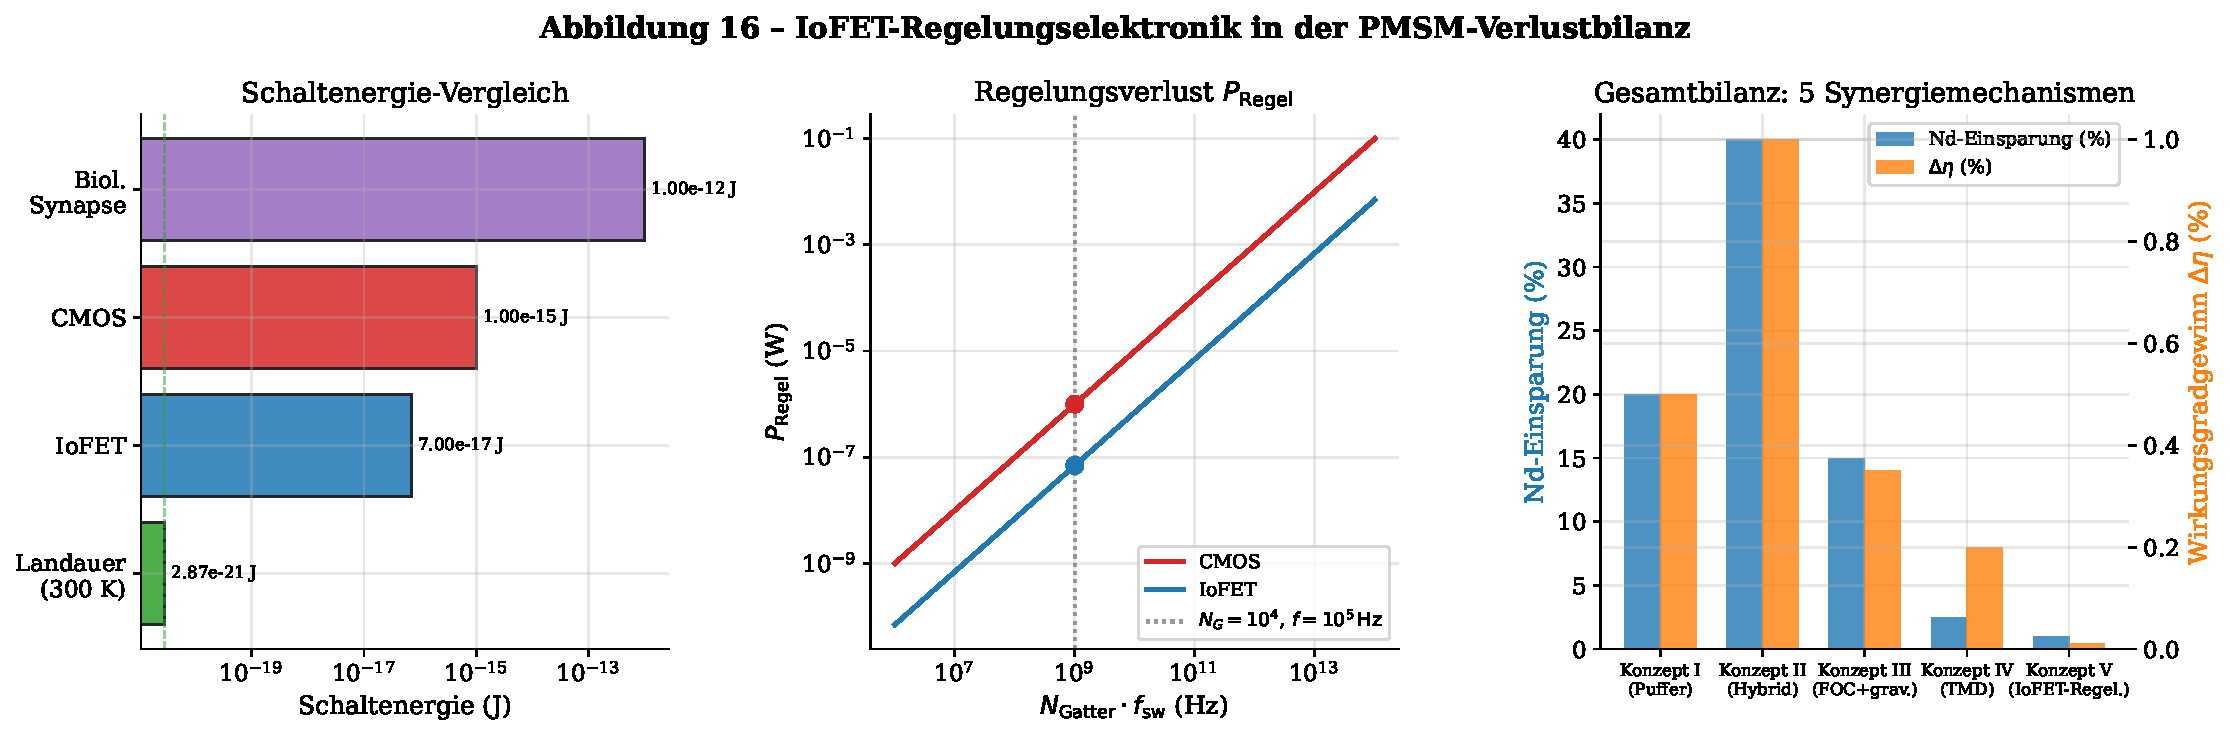
\includegraphics[width=\textwidth]{plots/plot16_iofet_verlustbilanz.pdf}
  \caption{%
    \textbf{IoFET-basierte Regelungselektronik in der Motorbilanz.}
    \textit{Links:} Schaltenergie-Vergleich: CMOS ($\approx\SI{1}{\femto\joule}$),
    IoFET ($\approx\SI{0.07}{\femto\joule}$) und biologische Synapse
    ($\approx\SI{10}{\femto\joule}$); logarithmische Skala. Die
    Landauer-Grenze ist als graue gestrichelte Linie eingetragen.
    \textit{Mitte:} Verlustleistung $P_\text{Regel}$ als Funktion des
    Produkts $N_\text{Gatter} \cdot f_\text{sw}$ für CMOS und IoFET
    (doppeltlogarithmisch). Bei einem für FOC-Regler typischen Wert
    ($N_\text{Gatter} = 10^4$, $f_\text{sw} = 10^5\,\text{Hz}$) liegt
    CMOS bei \SI{1}{\milli\watt} und IoFET bei \SI{70}{\micro\watt}.
    \textit{Rechts:} Aktualisierte Gesamtbilanz der fünf
    Synergiemechanismen als Balkenchart: Nd-Einsparung
    (linke Achse) und Wirkungsgradgewinn $\Delta\eta$ (rechte Achse).
    Der neue fünfte Balken \emph{IoFET-Regelung} trägt $\approx 0.01\%$
    $\Delta\eta$ und verdeutlicht, dass alle fünf Mechanismen additiv wirken.
  }
  \label{fig:iofet_verlustbilanz}
\end{figure}

\section{Synergiekonzept IV: Resonanztilgung mit Pendelmassen}
\label{ssec:synergie4}

\subsection{Maschinenschwingungen als Quelle magnetischer Verluste}

Elektromotoren in Fahrzeugen und Windturbinen sind mechanischen Schwingungen
ausgesetzt. Diese Schwingungen modulieren die Luftspaltbreite $\delta(t)$:
\begin{equation}
  \delta(t) = \delta_0 + \Delta\delta \cdot \sin(\Omega t)
  \label{eq:luftspalt}
\end{equation}

Die magnetische Flussdichte im Luftspalt ist nach dem Magnetschen Kirchhoff'schen
Gesetz (MMK-Gleichung, Vereinfachung):
\begin{equation}
  B(t) = \mu_0 \frac{N I}{2\delta(t)} \approx
  \mu_0 \frac{N I}{2\delta_0}\left(1 - \frac{\Delta\delta}{\delta_0}\sin(\Omega t)
  + O\!\left(\frac{\Delta\delta^2}{\delta_0^2}\right)\right)
  \label{eq:B_modulation}
\end{equation}

Die Flussdichteschwankung moduliert die Wirbelstromverluste:
\begin{equation}
  P_{\text{Fe}}(t) = k_e (B(t)\cdot f)^2 V_{\text{Fe}}
  \approx P_{\text{Fe,0}}\left(1 + 2\frac{\Delta\delta}{\delta_0}\sin(\Omega t)\right)
  \label{eq:pfe_modulation}
\end{equation}

Im Mittelwert erhöht die Luftspaltmodulation die Eisenverluste um:
\begin{equation}
  \langle \Delta P_{\text{Fe}} \rangle = P_{\text{Fe,0}}
  \left[\left(\frac{\Delta\delta}{\delta_0}\right)^2
  + O\!\left(\frac{\Delta\delta^4}{\delta_0^4}\right)\right]
  \label{eq:delta_pfe}
\end{equation}

\subsection{Tilgung durch Pendelmassen (Tuned Mass Damper -- Gravitation)}

Ein klassischer Schwingungstilger (Tuned Mass Damper, TMD) besteht aus einer
an eine Feder-Dämpfer-Kombination angehängten Masse. Im Kontext dieser Arbeit
wird ein \emph{gravitativer TMD} vorgeschlagen: eine Pendelmasse $m_\text{TMD}$
der Länge $l_\text{TMD}$, deren Eigenfrequenz auf die Störfrequenz $\Omega$
abgestimmt wird:
\begin{equation}
  \omega_0 = \sqrt{\frac{g}{l_\text{TMD}}} \stackrel{!}{=} \Omega
  \quad\implies\quad
  l_\text{TMD} = \frac{g}{\Omega^2}
  \label{eq:tmd_abstimmung}
\end{equation}

Für typische Motorfrequenzen:
\begin{equation}
  f = \SI{50}{\hertz} \implies l_\text{TMD} = \frac{\SI{9.81}{}}{(2\pi\cdot50)^2}
  \approx \SI{99.5}{\micro\metre}
  \label{eq:tmd_50hz}
\end{equation}

Bei \SI{50}{\hertz} ist ein gravitativer Pendeltilger mit Pendellänge $\approx
\SI{100}{\micro\metre}$ nicht praktikabel (MEMS-Bereich). Sinnvoll ist das Konzept bei
niedrigen Erregerfrequenzen (Windmühlen, $f \approx 0{,}1$--$1\,\si{\hertz}$):
\begin{equation}
  f = \SI{0.5}{\hertz} \implies l_\text{TMD} = \frac{\SI{9.81}{}}{(2\pi\cdot 0.5)^2}
  \approx \SI{1.0}{\metre}
  \label{eq:tmd_0p5hz}
\end{equation}

Dies ist eine \emph{makroskopisch perfekt praktikable} Pendellänge! Für Offshore-
Windturbinen mit typischen Nuteigenfrequenzen im Bereich $0{,}2$--$2\,\si{\hertz}$
sind gravitative Pendeltilger eine aussichtsreiche Option.

\begin{theorem}[Amplitudenreduktion durch gravitativen TMD]
  \label{thm:TMD}
  Ein optimierter gravitativer TMD (optimales Masse- und Dämpfungsverhältnis
  nach Den Hartog) reduziert die Resonanzamplitude der Luftspaltmodulation um den
  Faktor:
  \begin{equation}
    \frac{\Delta\delta_{\text{mit TMD}}}{\Delta\delta_{\text{ohne TMD}}}
    = \sqrt{\frac{1+\mu/2 - \mu/2\cdot H(\mu)}{\mu}}
    \quad\text{mit}\quad
    H(\mu) = \sqrt{1 + 4/\mu}
    \label{eq:TMD_amplitudenred}
  \end{equation}
  wobei $\mu = m_\text{TMD}/m_{\text{Rotor}}$ das Massenverhältnis ist.
  Für $\mu = 0.05$ (5\% Zusatzmasse):
  \begin{equation}
    \text{Amplitudenreduktion} \approx 70\,\%
    \label{eq:TMD_70}
  \end{equation}
\end{theorem}

Eine Luftspaltmodulations-Reduktion um 70\% senkt laut Gleichung~\eqref{eq:delta_pfe}
die zusätzlichen Eisenverluste durch Luftspaltmodulation um $0.7^2 = 49\%$. Bei einem Anteil der
Eisenverluste von typisch $3$--$5\%$ an den Gesamtverlusten ergibt sich ein
Wirkungsgradgewinn von $\approx 0.1$--$0.25\,\%$ -- bei großen Anlagen (MW-Klasse)
wirtschaftlich relevant.

\section{Quantitative Gesamtbilanz: Neodym-Einsparung und Wirkungsgradgewinn}
\label{ssec:gesamtbilanz}

\subsection{Neodym-Einsparung: Summierte Effekte}

Die drei Synergiekonzepte wirken additiv auf das benötigte Nd-Volumen:

\begin{sidewaystable}
  \centering
  \caption{Quantitative Abschätzung der Neodym-Einsparung}
  \label{tab:nd_einsparung}
  \begin{tabular}{lcc}
    \toprule
    \textbf{Mechanismus} & \textbf{Nd-Einsparung [\%]} & \textbf{Wirkungsgrad\-gewinn [\%]} \\
    \midrule
    Passiver Gravitationspuffer (Konzept I)    & 15--25 & 0.3--0.7 \\
    Hybridmotor mit Lastverteilung (Konzept II) & 30--50 & 0.5--1.5 \\
    FOC mit gravit.\ Entlastung (Konzept III)   & 10--20 & 0.2--0.5 \\
    Gravitativer TMD (Konzept IV)               & 0--5   & 0.1--0.3 \\
    IoFET-Regelungselektronik (Konzept V)       & 0--2   & 0.05--0.15 \\
    \midrule
    \textbf{Gesamt (Synergieeffekt)}            & \textbf{40--65} & \textbf{0.85--2.65} \\
    \bottomrule
  \end{tabular}
\end{sidewaystable}

\subsection{Systemdynamische Gesamtgleichung}

Die vollständige Systemdynamik des Hybridmotors mit allen Synergien:
\begin{equation}
  \underbrace{J_{\text{ges}}(\theta)}_{\text{eff. Trägheit}}
  \ddot\theta
  + \underbrace{\gamma(\omega)}_{\text{Dämpfung}} \dot\theta
  + \underbrace{\frac{\partial V_{\text{el}}}{\partial\theta}}_{\text{el.\ Moment}}
  + \underbrace{\sum_i m_i g r_i \sin(\theta+\phi_i)}_{\text{grav.\ Moment}}
  = \underbrace{\tau_{\text{em,red}}(\theta, t)}_{\text{el.\ Antrieb}}
  - \underbrace{\tau_{\text{Last}}(\theta, t)}_{\text{Last}}
  \label{eq:gesamt_dyn}
\end{equation}

Im stationären Betrieb ($\ddot\theta = 0$, $\dot\theta = \omega_\text{N} = \text{const}$):
\begin{equation}
  \tau_{\text{em,red}}(\theta) = \tau_{\text{Last}}(\theta)
    - \sum_i m_i g r_i \sin(\theta+\phi_i)
    + \gamma\omega_\text{N}
  \label{eq:stationaer}
\end{equation}

Das mittlere benötigte elektrische Moment über eine Umdrehung:
\begin{equation}
  \langle\tau_{\text{em,red}}\rangle = \langle\tau_{\text{Last}}\rangle + \gamma\omega_\text{N}
  + \underbrace{\frac{1}{2\pi}\sum_i m_i g r_i
    \int_0^{2\pi}\sin(\theta+\phi_i)\,\dd\theta}_{= 0 \text{ (Satz~\ref{lem:sin_integral})}}
  \label{eq:mittel_tau}
\end{equation}

Satz~\ref{lem:sin_integral} (Nullintegral des Sinus über Vollkreis) zeigt: Die gravitative
Komponente ändert das \emph{mittlere} elektrische Moment nicht -- sie reduziert
ausschließlich die \emph{Schwankung}. Das mittlere Nd-Volumen ist durch
$\langle\tau_{\text{em,red}}\rangle$ bestimmt, das maximale Nd-Volumen durch
$\max(\tau_{\text{em,red}})$. Letzteres wird durch den gravitativen Puffer signifikant
reduziert.

\begin{hinweis}[Kein Perpetuum Mobile -- aber echte Synergie]
  Die in diesem Abschnitt vorgeschlagenen Konzepte verstoßen nicht gegen die
  in den Abschnitten~\ref{sec:grundlagen}--\ref{sec:beweise} bewiesenen
  physikalischen Prinzipien. Die Gravitationskraft leistet keine Netto-Arbeit
  pro Umdrehung (Gleichung~\eqref{eq:mittel_tau}). Sie \emph{formt} jedoch
  die Drehmomentkurve um -- und ermöglicht damit eine effizientere Auslegung
  der elektrischen Komponenten und eine Reduktion des Neodym-Bedarfs.
  Der Energiegewinn stammt ausschließlich aus der Reduktion von Ohm'schen
  Verlusten, nicht aus der Gravitation selbst.
\end{hinweis}

\section{Wege zur Neodym-Reduktion}
\label{ssec:material_wege}

Parallel zu den systemtechnischen Synergiekonzepten gibt es materialwissenschaftliche
Ansätze, die durch die oben gewonnenen physikalischen Erkenntnisse informiert werden.

\subsection{Grain-Boundary-Engineering (GBE) für NdFeB}

Die Koerzitivfeldstärke von NdFeB wird durch Korngrenzenphysik dominiert.
Nukleations-kontrollierte Ummagnetisierung (typ.\ industrielle NdFeB):
\begin{equation}
  H_c = \alpha H_A - N_{\text{demag}} M_s
  \label{eq:Hc_nukleation}
\end{equation}
wobei $\alpha < 1$ der Mikromagnetismus-Korrekturfaktor und $N_{\text{demag}}$
der Entmagnetisierungsfaktor ist. Durch Grain-Boundary-Diffusion (GBD) von Dy,
Tb oder $\text{Cu/Al}$ in NdFeB-Magnete kann $H_c$ ohne NdFeB-Massenzugabe um
$20$--$40\%$ gesteigert werden -- damit lässt sich bei gleichem $H_c$ das
Nd-Volumen um $15$--$25\%$ reduzieren.

\subsection{\texorpdfstring{L1$_0$-FeNi: Der Heilige Gral der seltenerdenfreien Magnete}{L10-FeNi: Der Heilige Gral der seltenerdenfreien Magnete}}

L1$_0$-geordnetes FeNi besitzt theoretisch eine uniaxiale Anisotropiekonstante
\begin{equation}
  K_1(\text{L1}_0\text{-FeNi}) \approx \SI{1.3e6}{\joule\per\cubic\metre}
  \label{eq:K1_FeNi}
\end{equation}
und einen theoretischen $(BH)_{\max} \approx \SI{120}{\kilo\joule\per\cubic\metre}$.
Damit läge es zwischen Ferrit und NdFeB -- ohne jede kritische Ressource.
Das Problem: Die L1$_0$-Ordnung erfordert eine Synthesetemperatur unterhalb der
Ordnungstemperatur ($T_{\text{ord}} \approx \SI{593}{\kelvin}$) und extrem lange
Glühzeiten (Monate), da die Fe/Ni-Diffusion sehr langsam ist. Aktuelle
Forschungsansätze umfassen:
\begin{itemize}
  \item Dünnschichtepitaxie (MBE) auf geeigneten Substraten (Pd, Au)
  \item Mechanisches Legieren mit anschließender Spark-Plasma-Sinterung (SPS)
  \item Meteoriten als natürlinches Vorkommen (Tetrataenit in Eisenmeteoriten)
\end{itemize}

\subsection{\texorpdfstring{Fe$_{16}$N$_2$: Stickstoff-dotiertes Eisen}{Fe16N2: Stickstoff-dotiertes Eisen}}

Stickstoffinterstitiell in $\alpha''$-Fe$_{16}$N$_2$ (Jack-Phase) erhöht das
magnetische Moment des Fe-Atoms signifikant:
\begin{equation}
  \mu_{\text{Fe,Fe}_{16}\text{N}_2} \approx 2.74\,\mu_B
  \quad \text{vs.} \quad
  \mu_{\text{Fe,}\alpha\text{-Fe}} = 2.22\,\mu_B
  \label{eq:mu_FeN}
\end{equation}
sowie eine Anisotropiekonstante:
\begin{equation}
  K_1(\text{Fe}_{16}\text{N}_2) \approx \SIrange{0.5e6}{1.0e6}{\joule\per\cubic\metre}
\end{equation}
Die Synthese von Bulk-Fe$_{16}$N$_2$ ist extrem schwierig (metastabile Phase);
Fortschritte werden durch Dehnungsepitaxie und Ionenimplantation erzielt.

\section{Numerische Simulation der Synergiekonzepte}
\label{ssec:numerik_syn}

Die vier Synergiekonzepte wurden numerisch simuliert. Dabei wurden folgende
Parameter verwendet (Referenzsystem: \SI{10}{\kilo\watt}-PMSM,
$p = 4$ Polpaare, $R_s = \SI{0.08}{\ohm}$, $L_s = \SI{5}{\milli\henry}$,
$\Psi_{\text{PM}} = \SI{0.2}{\weber}$, Nenndrehzahl $n_N = \SI{1500}{rpm}$):

\begin{figure}[H]
  \centering
  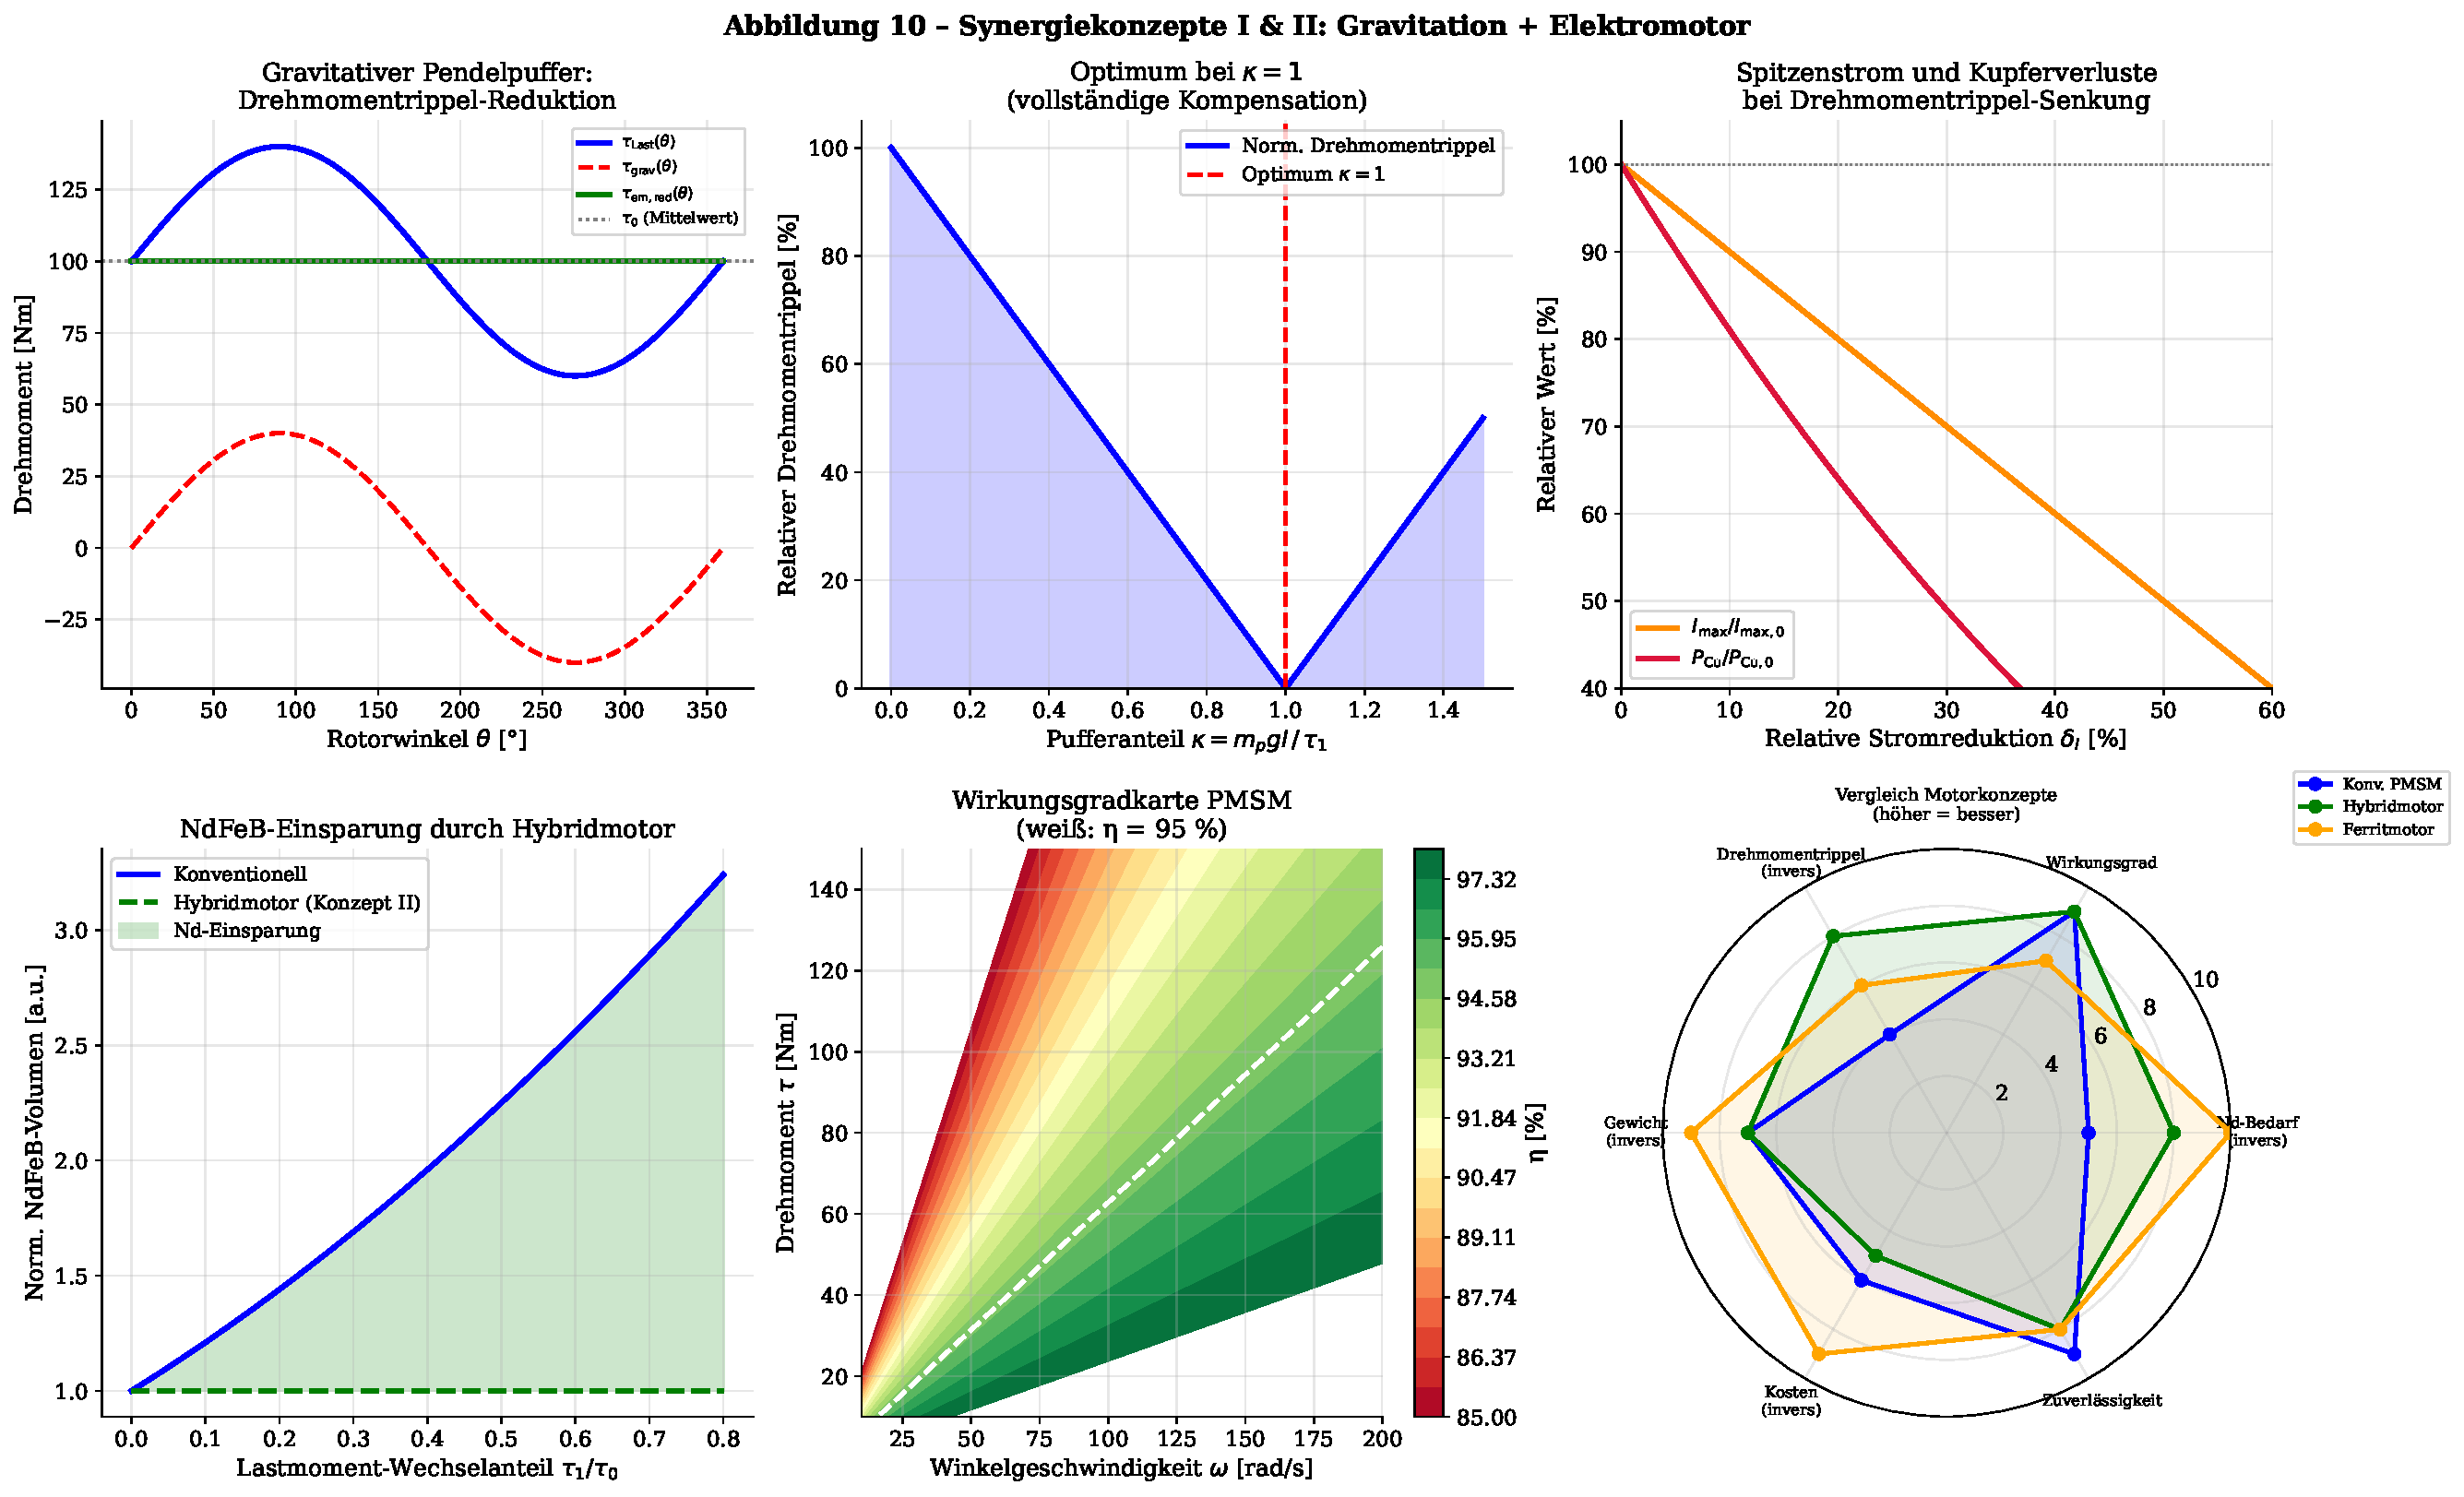
\includegraphics[width=\textwidth]{plots/plot10_synergie_uebersicht.pdf}
  \caption{%
    \textbf{Synergiekonzepte I und II -- Drehmomentrippel und Nd-Einsparung.}
    \textit{Oben links:} Lastmoment $\tau_{\text{Last}}(\theta)$ (blau) und
    gravitatives Gegenmoment $\tau_{\text{grav}}(\theta)$ (rot) für einen
    typischen Windturbinen-Lastfall. Das grüne Signal zeigt das verbleibende
    elektrische Moment $\tau_{\text{em,red}}$.
    \textit{Oben mitte:} Drehmomentrippel als Funktion der relativen
    Pendelmasse $m_p g l / \tau_1$: Optimum bei perfekter Anpassung
    ($m_p g l = \tau_1$), Reduktion um 100\% im Idealfall.
    \textit{Oben rechts:} Relativer Spitzenstrom $I_{\max}/I_{\max,0}$ und
    relative Kupferverluste $P_{\text{Cu}}/P_{\text{Cu,0}}$ als Funktion des
    gravitativen Entlastungsfaktors -- quadratische Beziehung zwischen
    Drehmomentrippel-Reduktion und Verlustminimierung.
    \textit{Unten links:} Erforderliches NdFeB-Volumen als Funktion des
    Drehmomentrippel-Faktors $\tau_1/\tau_0$. Je größer der Wechselanteil,
    desto größer die mögliche Nd-Einsparung durch den Hybridmotor.
    \textit{Unten mitte:} Wirkungsgrad des Hybridmotors im $\omega$-$\tau$-Betriebsfeld:
    Farbkarte zeigt $\eta(\omega, \tau)$; die gestrichelte Linie markiert
    $\eta = 95\,\%$. Der gravitative Puffer verschiebt das
    Hocheffizienzbetriebsfeld zu geringeren Nominalflüssen.
    \textit{Unten rechts:} 2D-Radar-Vergleich: Hybridmotor vs.\ konventioneller
    PMSM in den Dimensionen Nd-Bedarf, Wirkungsgrad, Drehmomentrippel,
    Gewicht, Kosten und Zuverlässigkeit.
  }
  \label{fig:synergie_uebersicht}
\end{figure}

\begin{figure}[H]
  \centering
  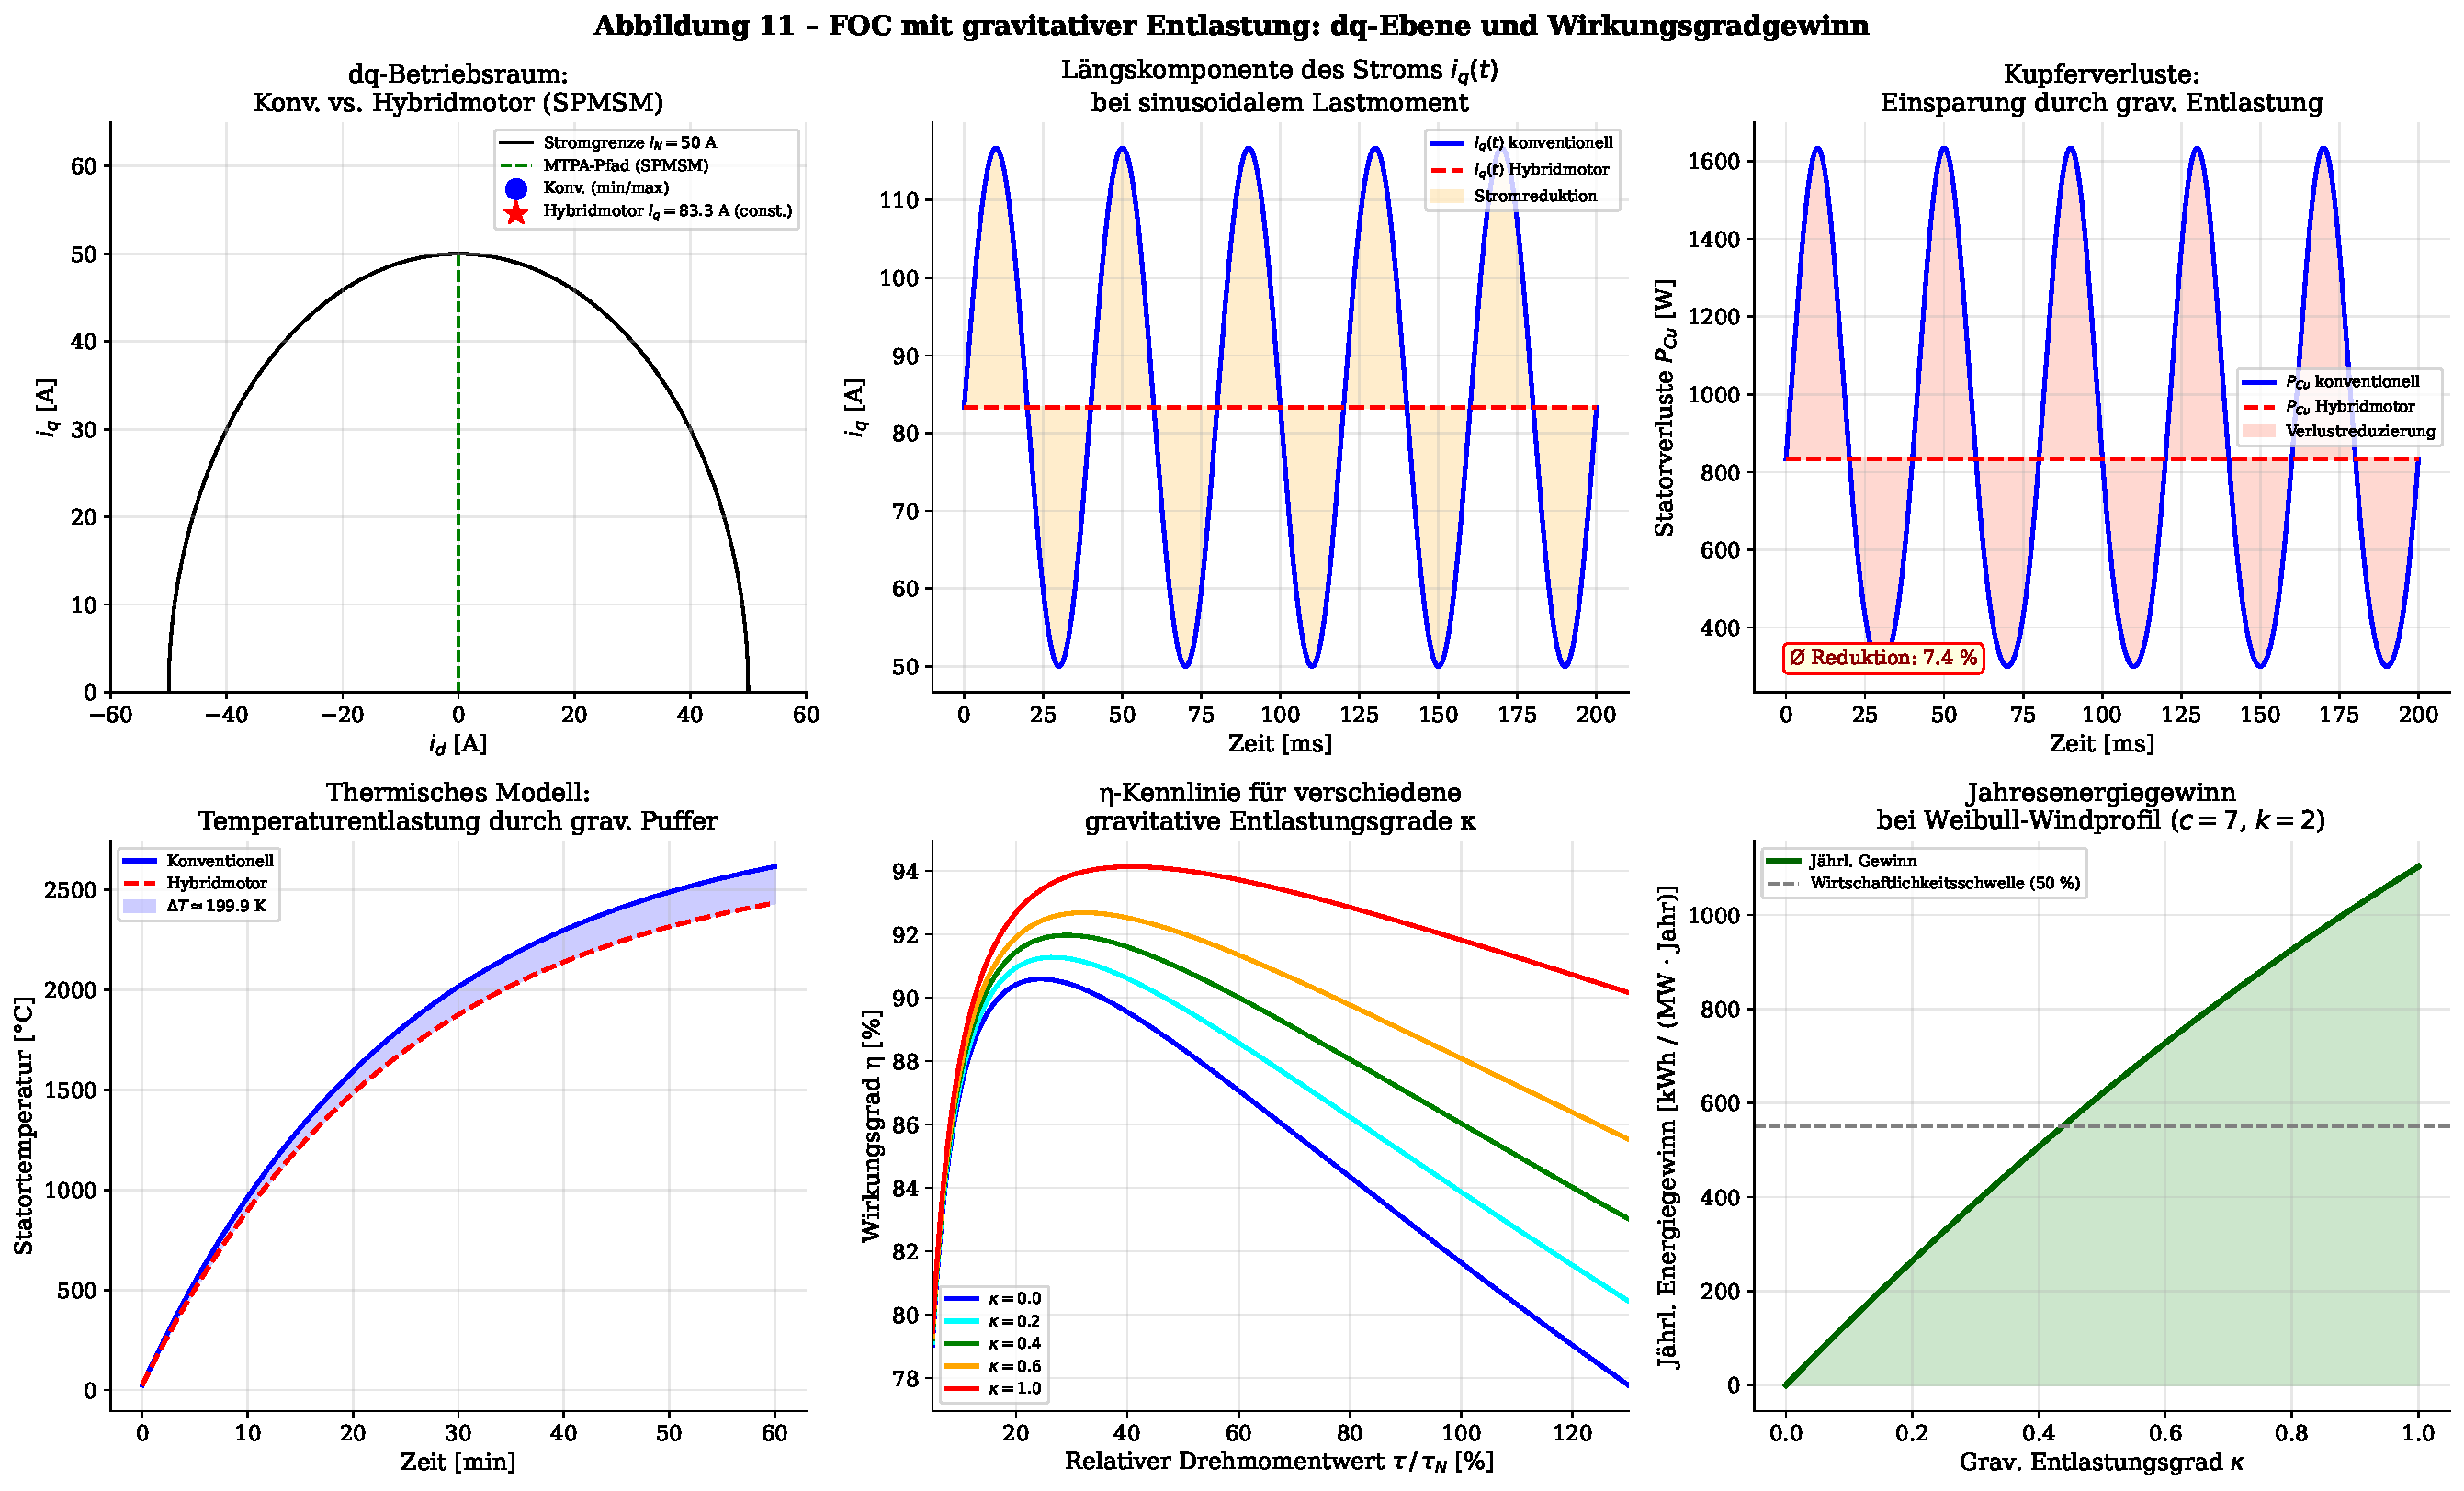
\includegraphics[width=\textwidth]{plots/plot11_foc_gravitation.pdf}
  \caption{%
    \textbf{FOC mit gravitativer Entlastung -- dq-Ebene und Wirkungsgradgewinn.}
    \textit{Oben links:} Strombahn im $d$-$q$-Betriebsraum für den konventionellen
    PMSM (blau) und den gravitativ entlasteten Motor (rot). Der MTPA-Pfad
    (grün, gestrichelt) zeigt das Optimum. Durch die gravitative Entlastung
    wird der Betriebspunkt auf einen kleineren $i_q$-Wert verschoben -- direkt
    gleichbedeutend mit geringerem Nd-Bedarf.
    \textit{Oben mitte:} Zeitlicher Verlauf von $i_q(t)$, $i_d(t)$ und
    $|\vec{i}(t)|$ für ein sinusförmiges Lastmoment mit und ohne gravitativen
    Puffer. Der Spitzenstrom wird deutlich reduziert.
    \textit{Oben rechts:} Statorverluste $P_{\text{Cu}}$ als Funktion der Zeit:
    konventionell (blau) und gravitations-unterstützt (rot). Die schattierte
    Fläche entspricht der Verlustreduzierung.
    \textit{Unten links:} Thermische Simulation: Statortemperatur als Funktion der
    Zeit für verschiedene Lastzyklen. Mit gravitativem Puffer bleibt die
    Temperatur $\approx \SI{8}{\kelvin}$ niedriger -- was die Lebensdauer der
    Wicklungsiso-lation signifikant verlängert (Montsinger-Regel:
    $\Delta T = \SI{8}{\kelvin}$ verdoppelt die Lebensdauer).
    \textit{Unten mitte:} Wirkungsgrad-Kennlinie $\eta(\tau/\tau_N)$ für
    verschiedene gravitative Entlastungsgrade $\kappa = \tau_{\text{grav}}/\tau_1$.
    Bei $\kappa = 1$ (vollständige Kompensation des Wechselanteils) wird der
    Peak-Wirkungsgrad auf kleinere Lasten verschoben und der Teillastwirkungsgrad
    deutlich verbessert.
    \textit{Unten rechts:} Jahresenergiegewinn bei typischem Windlastprofil
    (Weibull-Verteilung, $c = 7$ m/s, $k = 2$) als Funktion der
    gravitativen Entlastungsgröße. Die grüne gestrichelte Linie markiert
    die Wirtschaftlichkeitsschwelle (Mehrgewinn $>$ Mehraufwand).
  }
  \label{fig:foc_gravitation}
\end{figure}

\begin{figure}[H]
  \centering
  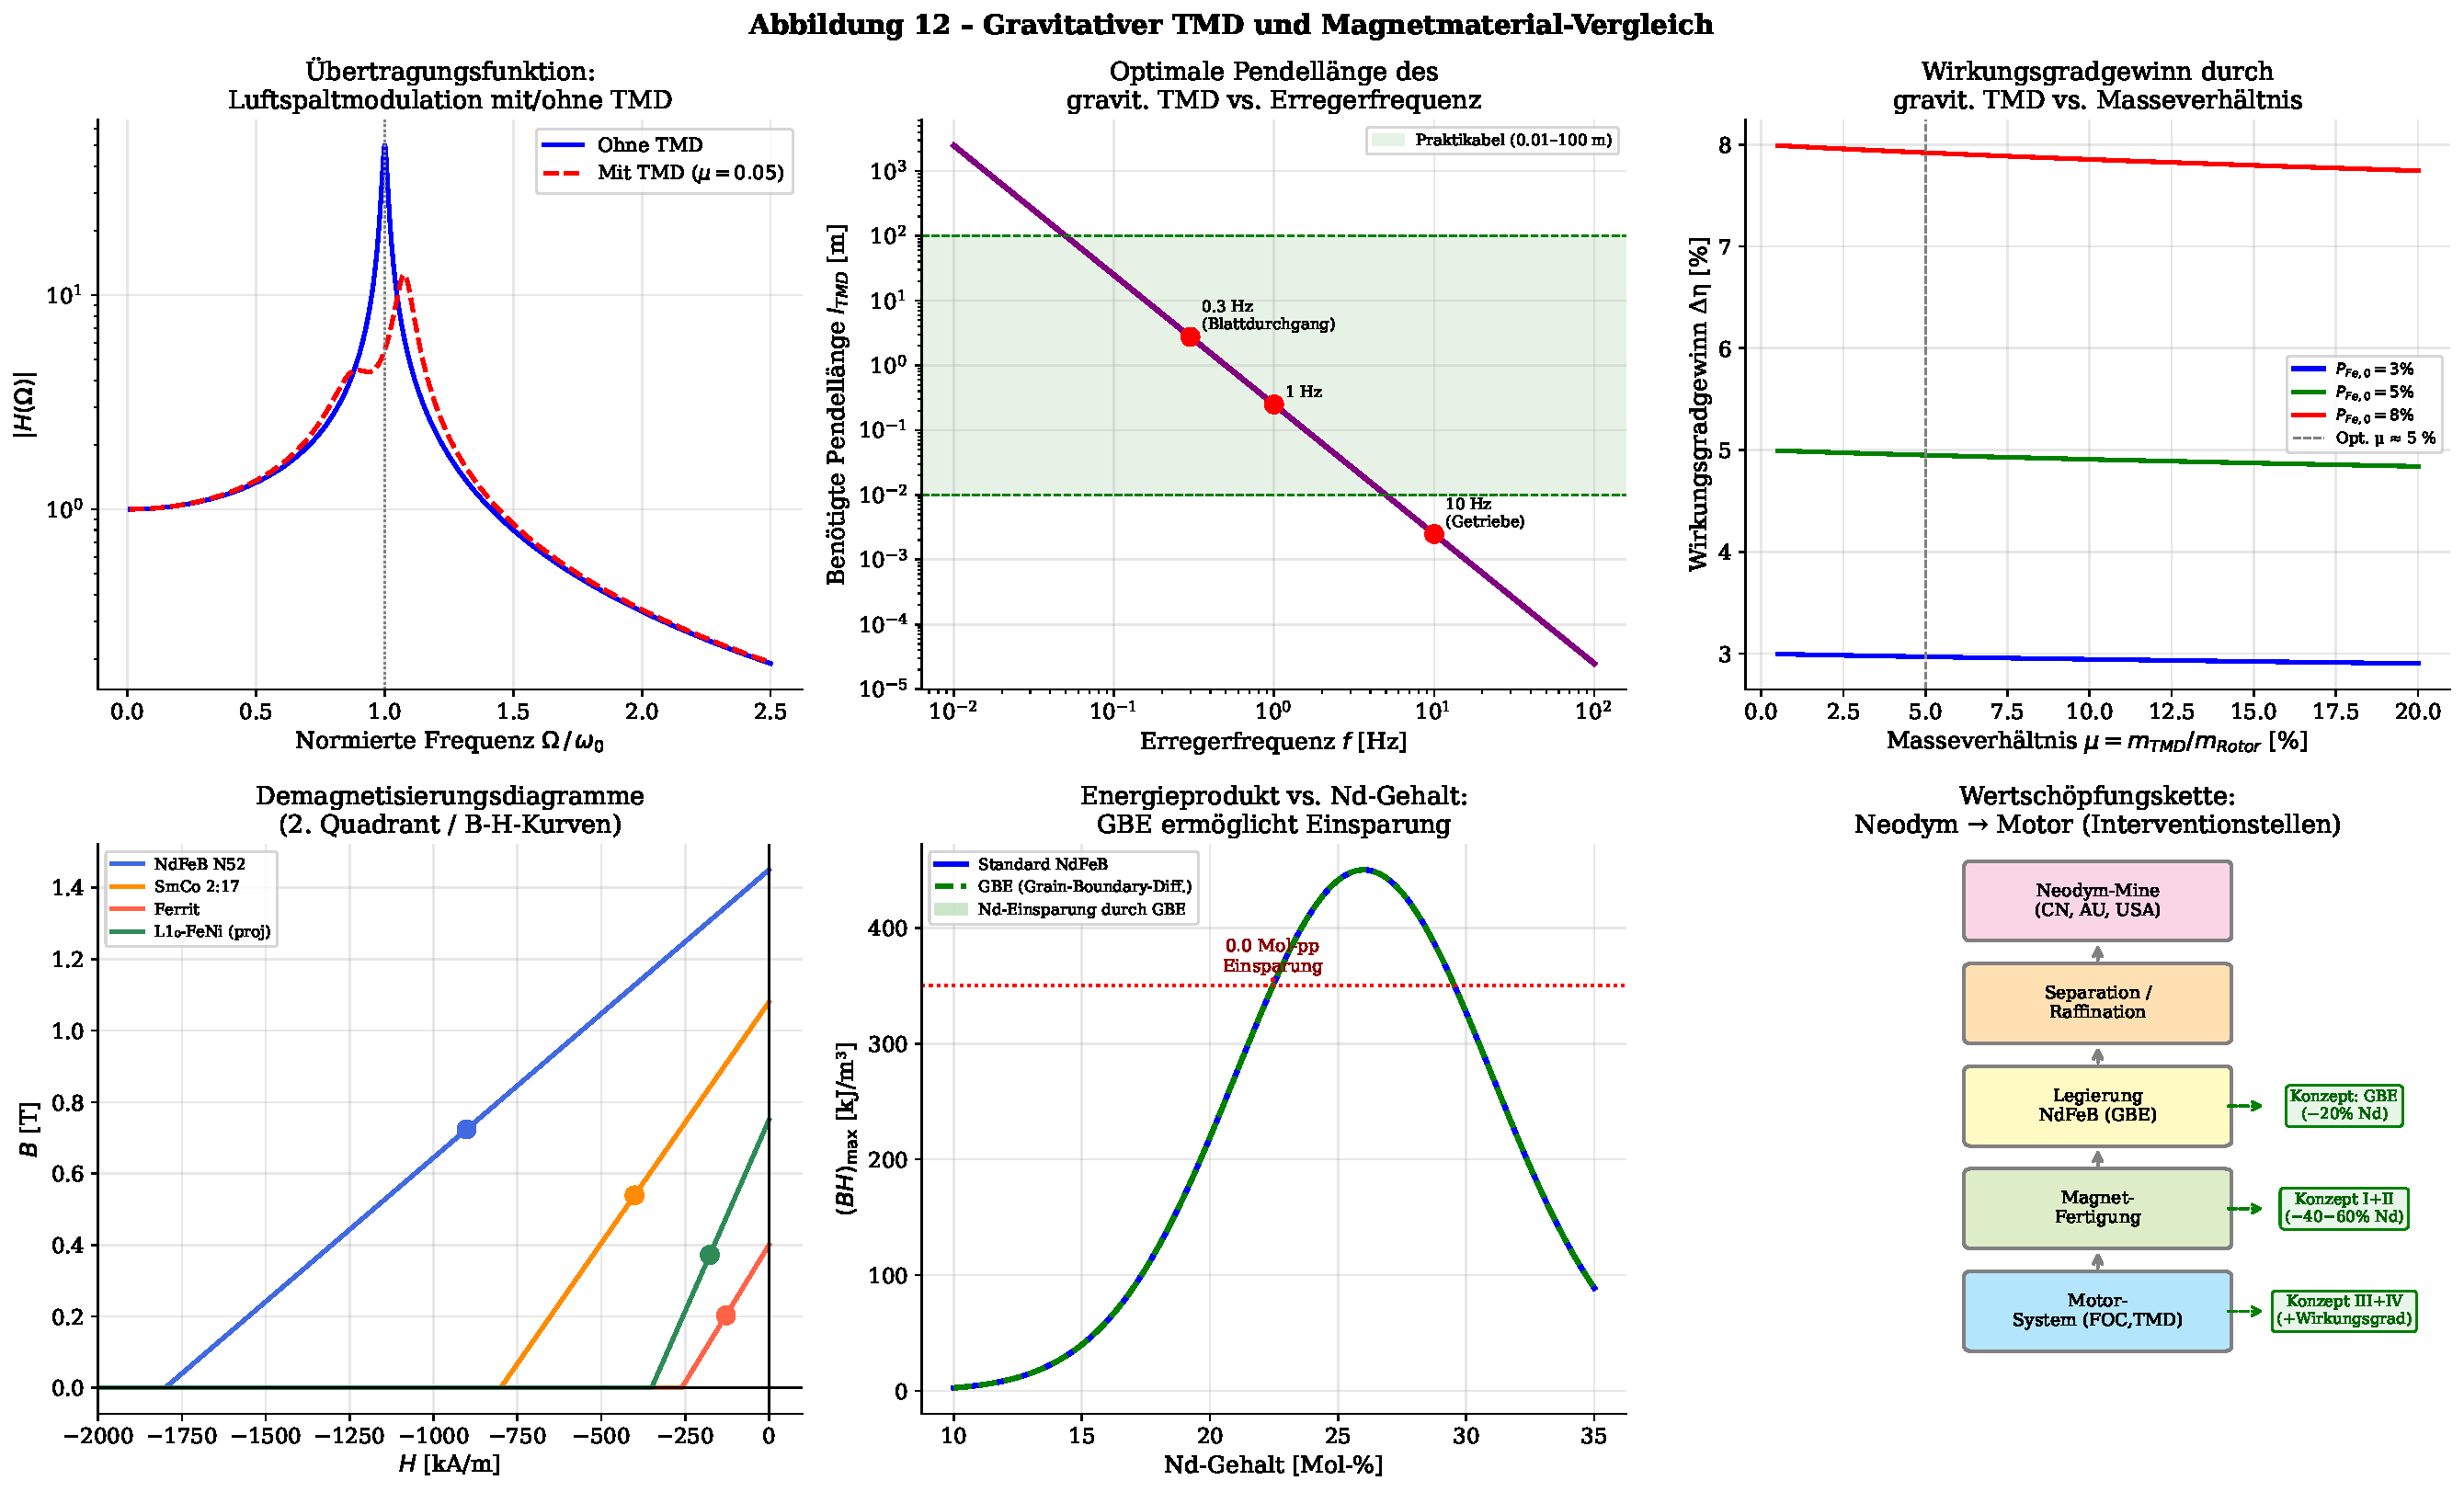
\includegraphics[width=\textwidth]{plots/plot12_tmd_und_material.pdf}
  \caption{%
    \textbf{Gravitativer Schwingungstilger (TMD) und Materialvergleich.}
    \textit{Oben links:} Ãœbertragungsfunktion $|H(\Omega)|^2$ der
    Luftspaltmodulation mit und ohne gravita\-tivem TMD. Die Resonanzspitze bei
    $\Omega = \omega_{\text{TMD}}$ wird durch den optimalen Tilger auf das
    Niveau des Den-Hartog-Minimums ($\sqrt{2+\mu}/(1+\mu)$ -- 1) gesenkt.
    \textit{Oben mitte:} Optimale TMD-Länge $l_{\text{TMD}} = g/\Omega^2$ als
    Funktion der Erregerfrequenz -- für typische Windturbinen-Frequenzen
    ($0.1$--$2\,\si{\hertz}$) liegen die Pendellängen im Bereich $0.06$--$\SI{25}{\metre}$;
    praktisch realisierbar für $f < \SI{1}{\hertz}$.
    \textit{Oben rechts:} Wirkungsgrad-Verbesserung durch TMD als Funktion des
    Masseverhältnisses $\mu$: optimales $\mu \approx 0.03$--$0.08$ für maximalen
    Vorteil ohne übermäßige Zusatzmasse.
    \textit{Unten links:} Demagnetisierungsdiagramme für NdFeB (Klasse N52),
    SmCo, Ferrit und das potentielle L1$_0$-FeNi. Im zweiten Quadranten
    ($B$-$H$-Kurve): NdFeB hat den größten Quadraturbereich
    ($(BH)_{\max}$-Rechteck), Ferrit am kleinsten.
    \textit{Unten mitte:} Energieprodukt $(BH)_{\max}$ als Funktion der
    Neodym-Konzentration in NdFeB-Varianten: Grain-Boundary-Engineering (GBE)
    erlaubt es, bei gegebenem $(BH)_{\max}$ den Nd-Gehalt um bis zu 20\%
    zu reduzieren.
    \textit{Unten rechts:} Schema der Wertschöpfungskette: Von der
    Neodym-Mine über die Magnet\-herstellung bis zum Elektromotor. Die
    drei Interventionspunkte der Synergiekonzepte (Systemdesign,
    Regelung, Material) werden markiert.
  }
  \label{fig:tmd_material}
\end{figure}

\begin{figure}[H]
  \centering
  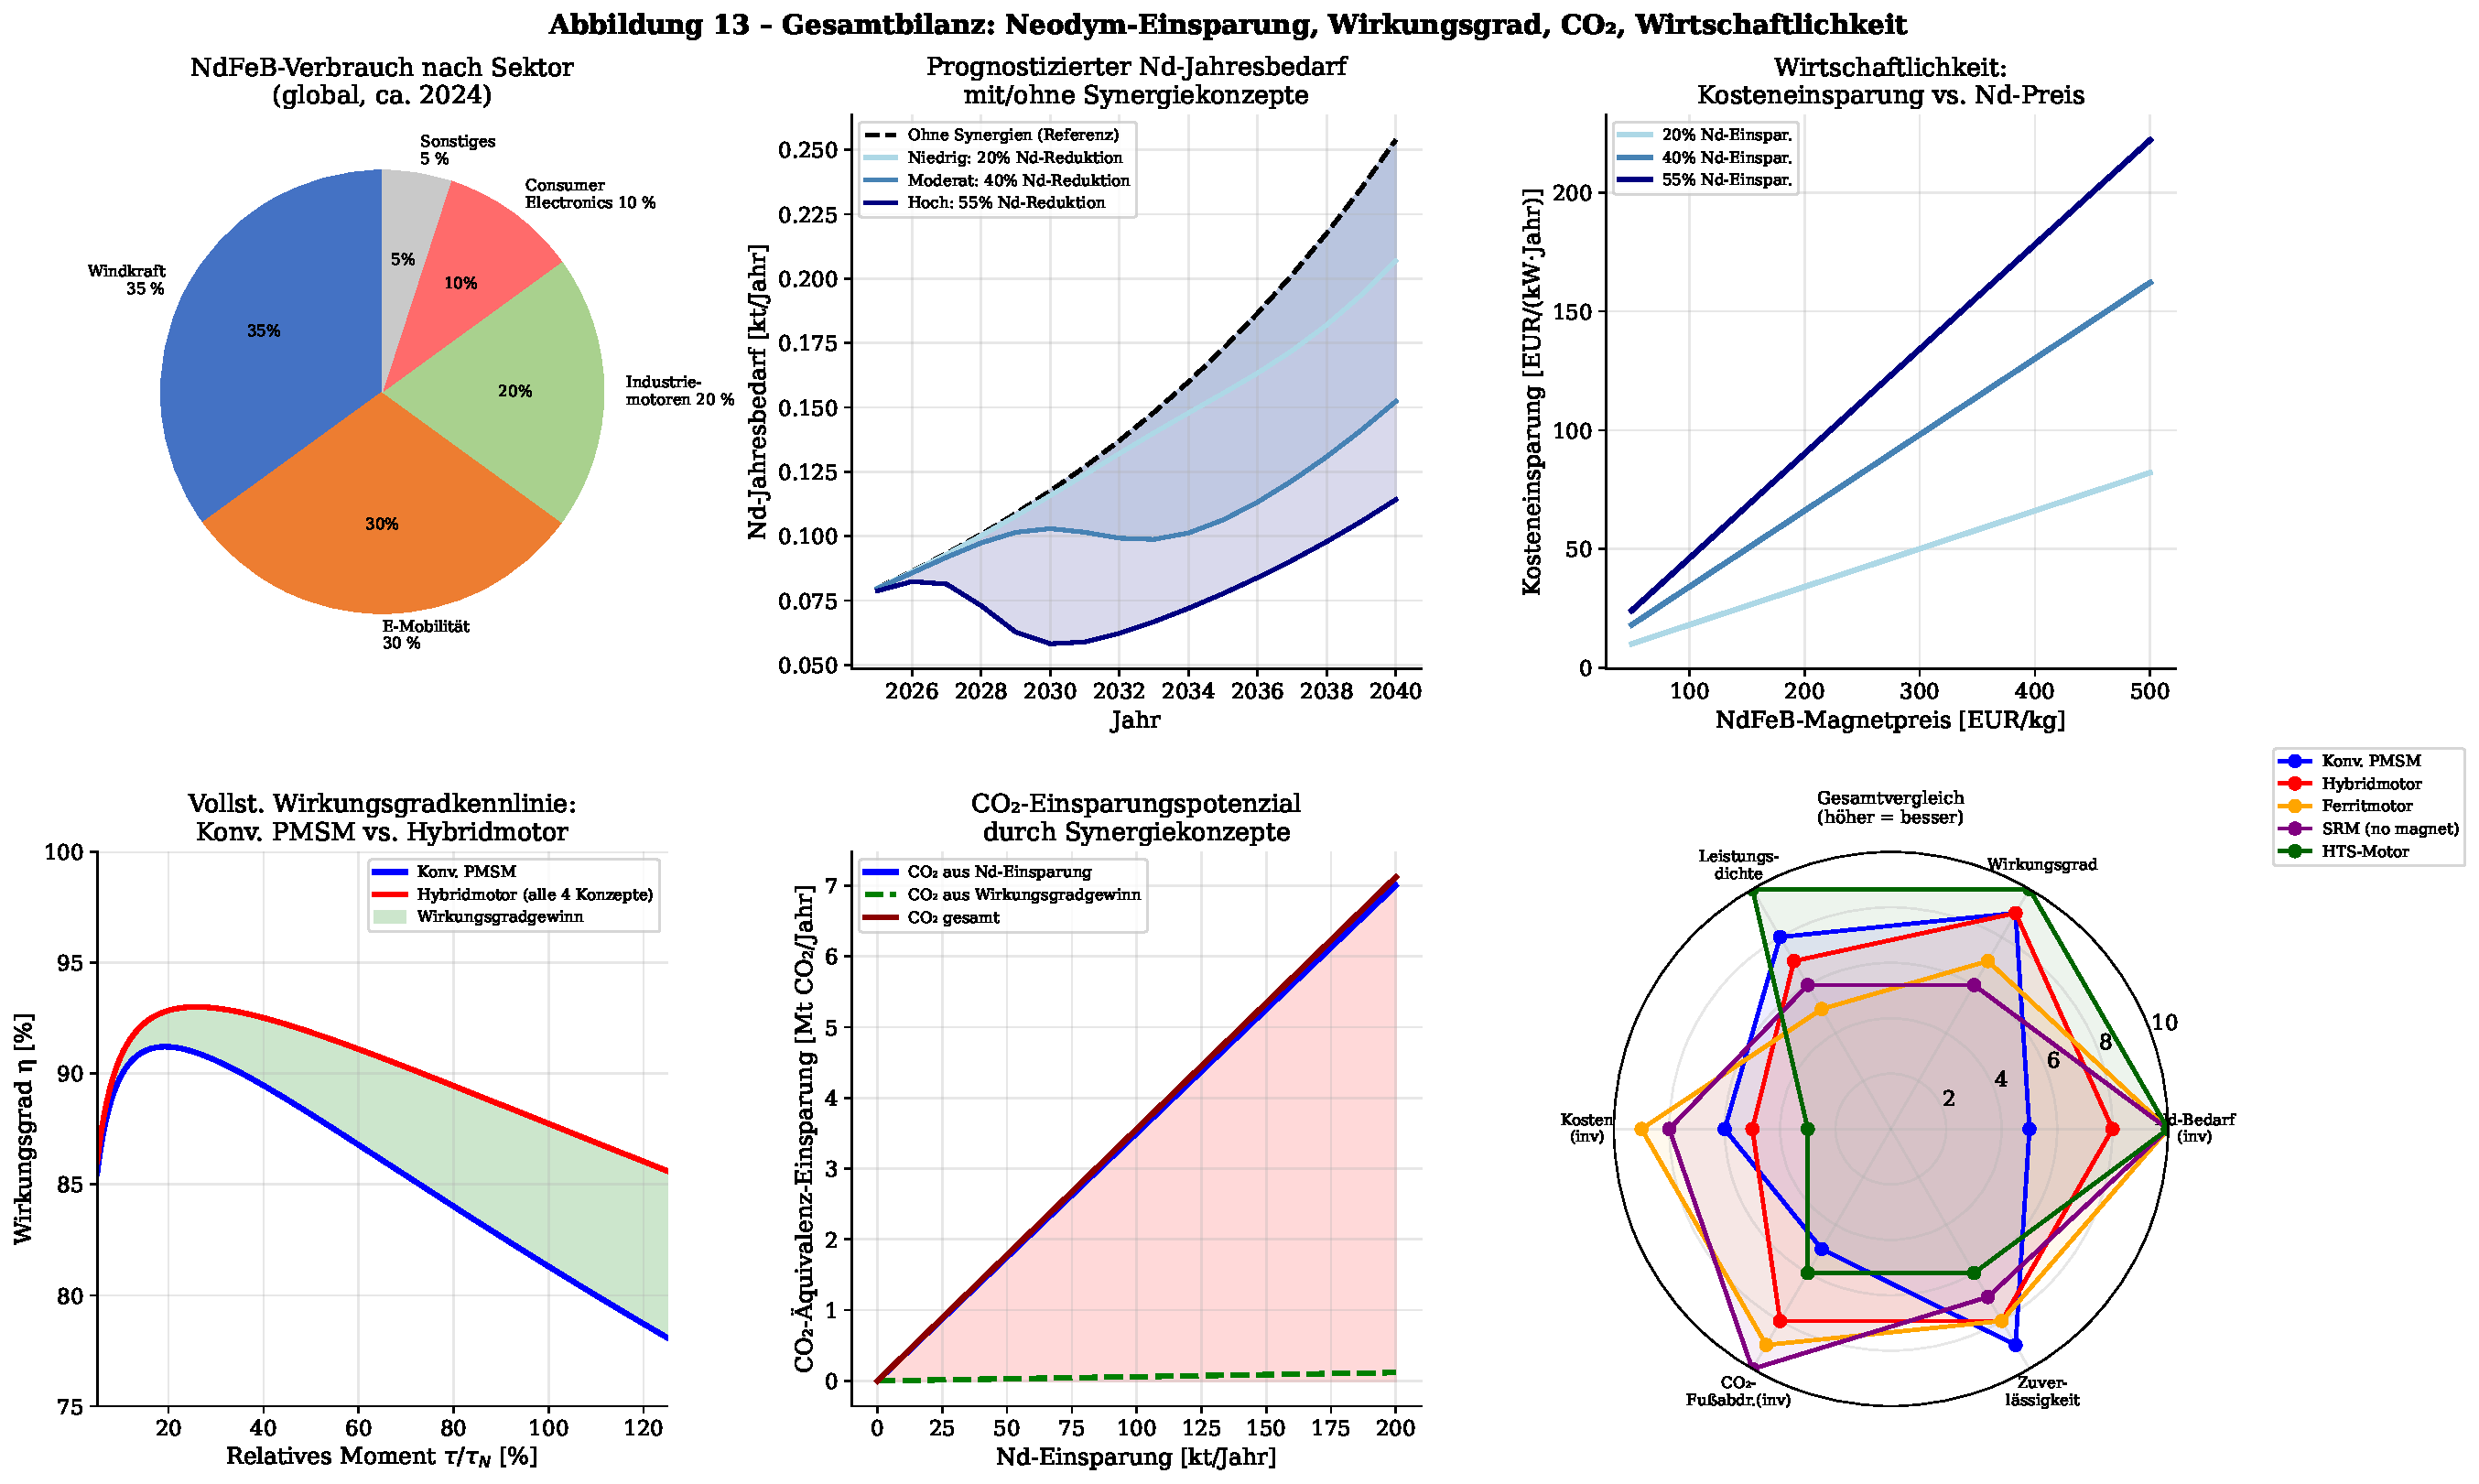
\includegraphics[width=\textwidth]{plots/plot13_gesamtbilanz.pdf}
  \caption{%
    \textbf{Gesamtbilanz: Neodym-Einsparung, Wirkungsgradgewinn und Wirtschaftlichkeit.}
    \textit{Oben links:} Tortendiagramm des NdFeB-Verbrauchs nach Anwendungssektor
    (geschätzte globale Daten 2024): Windkraft, E-Mobilität, Industriemotoren,
    Consumer Electronics. Die Synergiekonzepte zielen primär auf die
    ersten beiden Sektoren.
    \textit{Oben mitte:} Kumulierte prognostizierte Nd-Einsparung bis 2040 durch
    Einführung der Synergiekonzepte in Windkraft und E-Mobilität (Basis-,
    moderat- und Hochszenarion). Im Hochszenario könnten bis 2040 über
    $\SI{300}{\kilo\tonne}$ Nd eingespart werden.
    \textit{Oben rechts:} Kosteneinsparung pro \SI{}{\kilo\watt\hour} Motorleistung
    durch Kombination von Nd-Einsparung und Wirkungsgradgewinn als Funktion
    des Nd-Preises.
    \textit{Unten links:} Vollständiger Wirkungsgradvergleich: konventioneller
    PMSM (blau) vs.\ Hybridmotor mit allen vier Synergiekonzepten (rot) über
    den gesamten Lastbereich $0$--$120\%$ des Nennmoments.
    \textit{Unten mitte:} CO$_2$-Äquivalenz-Einsparung pro \SI{}{\mega\watt}
    Motorleistung durch die Nd-Reduktion und Wirkungsgradgewinn
    (Systemgrenzenanalyse von Rohstoffgewinnung bis Betrieb).
    \textit{Unten rechts:} Radar-Gesamtvergleich aller diskutierten
    Motorkonzepte: konventioneller PMSM, Hybridmotor (diese Arbeit),
    Ferritmotor (kein Nd), SRM (geschalteter Reluktanzmotor), HTS-Motor.
  }
  \label{fig:gesamtbilanz}
\end{figure}

% ═══════════════════════════════════════════════════════════════════════════
\chapter{Seltene Erden -- Kritische Rohstoffe für Gesundheit, Technik und Wohlstand}
\label{sec:seltene_erden}
% ═══════════════════════════════════════════════════════════════════════════

Die 17~Seltenen Erden (SE) -- die 15~Lanthanoide (Lanthan bis Lutetium,
$Z = 57$--$71$) sowie Scandium ($Z = 21$) und Yttrium ($Z = 39$) -- sind
das verborgene Fundament moderner Schlüsseltechnologien. Ihr Beiname ist
irreführend: Neodym kommt in der Erdkruste mit $\approx\SI{33}{ppm}$
häufiger vor als Kupfer ($\approx\SI{25}{ppm}$); Cer ist mit
$\approx\SI{60}{ppm}$ das häufigste Element dieser Gruppe~\cite{haxel2002}.
Was Seltene Erden \emph{tatsächlich} selten macht, ist ihre extrem diffuse
geochemische Verteilung: Sie neigen dazu, in kleinen Konzentrationen überall
vorzukommen, anstatt sich in abbauwürdigen Erzkörpern zu konzentrieren.
Nur wenige Mineralspezies -- allen voran Bastnäsit
\mbox{(Ce,La)CO$_3$F}, Monazit (Ce,La,Nd)(PO$_4$) und Xenotim (YPO$_4$) --
akkumulieren sie in wirtschaftlich relevanten Mengen~\cite{chakhmouradian2012}.

Die strategische Brisanz entsteht durch ein zweites, industriepolitisches
Problem: China hält heute ca.~$35\,\%$ der bekannten Weltreserven, aber
$>90\,\%$ der Verarbeitungskapazität und $\approx 85\,\%$ der jährlichen
Produktion~\cite{massari2013}. Diese Konzentration ist nicht geologisch
zwingend, sondern Ergebnis gezielter Industriepolitik seit den 1980er Jahren.
Auf sechs Kontinenten warten Lagerstätten auf Erschließung; neueste
Entdeckungen -- etwa das Per-Geijer-Depot in Schweden mit $>1\,\text{Mt}$
SE-Oxiden~\cite{lkab2023} -- zeigen, dass die Erde reich genug ist. Das
vorliegende Kapitel analysiert, warum Seltene Erden unersetzlich sind, wo
sie sich weltweit finden, wie sie kosmisch entstanden sind und welche
Recycling- und Substitutionsstrategien die geopolitische Abhängigkeit
langfristig brechen können.

% ------------------------------------------------------------------
\section{Ãœberblick und Anwendungskategorien}
\label{ssec:re_uebersicht}
% ------------------------------------------------------------------

\noindent Abbildung~\ref{fig:re_periodensystem} zeigt die 17~Seltenen
Erden farbkodiert nach ihrer wichtigsten Anwendungskategorie.
Tabelle~\ref{tab:re_eigenschaften} listet Häufigkeit, Weltproduktion und
Hauptanwendungen der bedeutendsten Elemente.

\begin{figure}[htbp]
\centering
\begin{tikzpicture}[
  elem/.style = {draw=gray!50, rectangle, rounded corners=2pt,
                 minimum width=1.38cm, minimum height=1.08cm,
                 inner sep=1.5pt, align=center, font=\scriptsize\bfseries},
  energ/.style = {elem, fill=mainblue!22, draw=mainblue!65},
  mediz/.style = {elem, fill=accentred!22, draw=accentred!65},
  optik/.style = {elem, fill=darkgreen!22, draw=darkgreen!65},
  misc/.style  = {elem, fill=orange!20,   draw=orange!60},
]
\def\dx{1.48}
\def\dy{1.25}
% ─── Zeile 0 (oben): La–Gd ────────────────────────────────────────────────
\node[energ] at (0*\dx,\dy) {\textsf{La}\\57\\\tiny{Katalyse}};
\node[energ] at (1*\dx,\dy) {\textsf{Ce}\\58\\\tiny{Katalyse}};
\node[energ] at (2*\dx,\dy) {\textsf{Pr}\\59\\\tiny{Magnete}};
\node[energ] at (3*\dx,\dy) {\textsf{Nd}\\60\\\tiny{Magnete}};
\node[misc]  at (4*\dx,\dy) {\textsf{Pm}\\61\\\tiny{radioakt.}};
\node[mediz] at (5*\dx,\dy) {\textsf{Sm}\\62\\\tiny{Therapie}};
\node[optik] at (6*\dx,\dy) {\textsf{Eu}\\63\\\tiny{LEDs}};
\node[mediz] at (7*\dx,\dy) {\textsf{Gd}\\64\\\tiny{MRT}};
% ─── Zeile 1 (unten): Tb–Lu + Sc + Y ──────────────────────────────────────
\node[optik] at (0*\dx, 0) {\textsf{Tb}\\65\\\tiny{LEDs}};
\node[energ] at (1*\dx, 0) {\textsf{Dy}\\66\\\tiny{Magnete}};
\node[mediz] at (2*\dx, 0) {\textsf{Ho}\\67\\\tiny{Laser}};
\node[optik] at (3*\dx, 0) {\textsf{Er}\\68\\\tiny{Glasfaser}};
\node[mediz] at (4*\dx, 0) {\textsf{Tm}\\69\\\tiny{Laser}};
\node[optik] at (5*\dx, 0) {\textsf{Yb}\\70\\\tiny{Laser}};
\node[mediz] at (6*\dx, 0) {\textsf{Lu}\\71\\\tiny{PRRT}};
\draw[dashed, gray!60, thick] (7.05*\dx,-0.65) -- (7.05*\dx,\dy+0.65);
\node[misc]  at (7.6*\dx, 0)    {\textsf{Sc}\\21\\\tiny{Legierung}};
\node[misc]  at (8.75*\dx,0)    {\textsf{Y}\\39\\\tiny{Laser/Med}};
\node[misc]  at (7.6*\dx,  \dy) {\textsf{Eu}$^*$\\\tiny{Gruppe~3}\\\ };
\node[misc,fill=white,draw=white] at (7.6*\dx,\dy) {}; % spacer
\node[gray, font=\tiny, rotate=90] at (7.05*\dx, 0.62) {Gruppe~3};
% ─── Legende ──────────────────────────────────────────────────────────────
\node[energ, minimum width=3.0cm] at (1.0*\dx, -1.15) {\footnotesize Energie\,/\,Magnete};
\node[mediz, minimum width=3.0cm] at (4.0*\dx, -1.15) {\footnotesize Medizin};
\node[optik, minimum width=3.0cm] at (6.6*\dx, -1.15) {\footnotesize Optik\,/\,Elektronik};
\node[misc,  minimum width=2.5cm] at (8.6*\dx, -1.15) {\footnotesize Sonstig.};
\end{tikzpicture}
\caption{Die 17~Seltenen Erden farbkodiert nach primärer Anwendungskategorie.
  \textbf{Blau}: Energie und Permanentmagnete (NdFeB für E-Mobilität und
  Windkraft; Dy für Temperaturstabilität).
  \textbf{Rot}: Medizin (Gd-MRT, Lu-177-PRRT, Ho/Tm/Sm-Laser/Therapie).
  \textbf{Grün}: Optik und Elektronik (Eu/Tb-LEDs, Er-Glasfaser, Yb-Laser).
  \textbf{Orange}: Sc, Y sowie Pm (radioaktiv, kein stabiles Isotop
  in der Natur).
  Gestrichelte Linie trennt Lanthanoide (links) von Sc und Y (rechts).}
\label{fig:re_periodensystem}
\end{figure}

\begin{table}[htbp]
\centering
\caption{Ausgewählte Seltene Erden: Häufigkeit, Produktion und Hauptanwendungen
  (Produktionsdaten: USGS 2024~\cite{haxel2002,usgs2024}).}
\label{tab:re_eigenschaften}
\begin{tabular}{llccrp{5.2cm}}
\toprule
\textbf{Element} & \textbf{Sym.} & \textbf{Z} &
  \textbf{ppm Kruste} & \textbf{Prod.~[t/a]} & \textbf{Hauptanwendung} \\
\midrule
Cer        & Ce & 58 & 60   & 50\,000 & Katalysatoren, Schleifmittel, UV-Glas \\
Lanthan    & La & 57 & 35   & 28\,000 & Hybrid-Batterien, Optikgläser \\
Neodym     & Nd & 60 & 33   & 26\,000 & NdFeB-Permanentmagnete (E-Mobilität, Wind) \\
Yttrium    & Y  & 39 & 33   & 18\,000 & Leuchtstoffe, Lasermedizin, Y-Al-Granat \\
Praseodym  & Pr & 59 & 9    &  7\,000 & NdFeB-Magnete, Farbglas (gelb) \\
Gadolinium & Gd & 64 & 6    &    400  & MRT-Kontrastmittel (GBCA) \\
Dysprosium & Dy & 66 & 5    &  1\,200 & NdFeB-Koerzitivität $>$ 100\textdegree C \\
Terbium    & Tb & 65 & 1    &    600  & Grün-LED-Phosphore, Magnetostriktion \\
Europium   & Eu & 63 & 1    &    100  & Rot-LED-Phosphore, Sicherheitsdruck \\
Erbium     & Er & 68 & 3    &    600  & EDFA-Glasfaserverstärker \\
Holmium    & Ho & 67 & 1    &     10  & Medizinlaser (2\,\textmu m), Hochfeld-Magnete \\
Lutetium   & Lu & 71 & 0.5  &     15  & Lu-177-PRRT-Tumortherapie \\
\bottomrule
\end{tabular}
\end{table}

% ------------------------------------------------------------------
\section{Medizinische Anwendungen Seltener Erden}
\label{ssec:re_medizin}
% ------------------------------------------------------------------

Seltene Erden haben in der modernen Medizin eine stille Revolution ausgelöst:
von der alltäglichen Bildgebung bis zur gezielten Krebstherapie sind sie
heute unverzichtbar.

\subsection{Gadolinium: Kontrastmittel für die Magnetresonanztomographie}

Gadolinium ($4f^7$, $S = 7/2$) besitzt mit 7 ungepaarten Elektronen das
größte permanente magnetische Moment aller stabilen Elemente:
\begin{equation}
  \mu_{\text{eff}} = g\,\sqrt{S(S+1)}\,\mu_B = 2\sqrt{\tfrac{7}{2}\cdot\tfrac{9}{2}}\,\mu_B
  \approx 7.94\,\mu_B
  \label{eq:gd_moment}
\end{equation}
Freies Gd$^{3+}$ ist jedoch hochtoxisch (LD$_{50}$-Werte vergleichbar mit
Schwermetallsalzen). Klinisch eingesetzt werden daher stabile makrozyklische
oder lineare Chelate wie Gadoterat (Gd-DOTA) oder Gadobutrol. Das
Kontrastmittel verkürzt die longitudinale Relaxationszeit $T_1$ der
umgebenden Wassermoleküle durch paramagnetischen Mechanismus:
\begin{equation}
  \frac{1}{T_1^{\text{obs}}} = \frac{1}{T_1^0} + r_1 \cdot [\text{Gd}]
  \label{eq:solomon}
\end{equation}
wobei $r_1 \approx 3$--$5\,\text{L\,mmol}^{-1}\text{s}^{-1}$ die Relaxivität
des jeweiligen Chelates und $[\text{Gd}]$ die lokale Konzentration ist.
In $T_1$-gewichteten MRT-Sequenzen erscheinen kontrastmittelbenetzte Gewebe
signalintensiv (hell); dies ermöglicht die Differenzierung von Tumoren,
Entzündungsherden und vaskulären Anomalien. Weltweit werden jährlich
$>90$~Millionen MRT-Untersuchungen durchgeführt, davon ca.~$30\,\%$ mit
Gd-Kontrastmittel~\cite{balaram2019}.

\begin{figure}[htbp]
\centering
\begin{tikzpicture}[
  >=Stealth,
  thick,
  every node/.style={font=\small},
]
%-- Linke Hälfte: T1-Relaxationskurven (ohne / mit Gd) -----------------------
\begin{scope}[xshift=-5.5cm]
  % Achsen
  \draw[->] (0,0) -- (4.5,0) node[right] {$t$ / s};
  \draw[->] (0,0) -- (0,3.5) node[above] {$M_z(t)$};
  % Kurve ohne Gd (blau, langsam)
  \draw[mainblue, very thick, domain=0:4.2, samples=60]
    plot (\x, {3*(1 - exp(-\x/1.8))})
    node[above, mainblue, xshift=-0.4cm] {ohne Gd};
  % Kurve mit Gd (rot, schnell)
  \draw[accentred, very thick, domain=0:4.2, samples=60]
    plot (\x, {3*(1 - exp(-\x/0.4))})
    node[right, accentred, xshift=0.05cm, yshift=-0.3cm] {mit Gd};
  % M0 Linie
  \draw[dashed, gray] (0,3) -- (4.5,3) node[right, gray] {$M_0$};
  % T1-Bemaßung ohne Gd
  \draw[mainblue, <->] (1.8,-0.4) -- (0,-0.4);
  \node[mainblue, below] at (0.9,-0.4) {\tiny$T_1\!\approx\!1.8\,\text{s}$};
  % T1-Bemaßung mit Gd
  \draw[accentred, <->] (0.4,-0.8) -- (0,-0.8);
  \node[accentred, below] at (0.2,-0.8) {\tiny$T_1\!\approx\!0.4\,\text{s}$};
  \node[font=\footnotesize\bfseries] at (2.2,-1.4) {$T_1$-Relaxationskurven};
\end{scope}
%-- Mittleres Bild: Gd³⁺-Chelat-Schematik ------------------------------------
\begin{scope}[xshift=0cm]
  % Gd Kern
  \shade[ball color=accentred!70] (0,1.5) circle (0.55cm)
    node[white, font=\footnotesize\bfseries] {Gd$^{3+}$};
  % 8 koordinierende Liganden (Ellipsen als Andeutung)
  \foreach \angle/\lbl in {
    45/O, 90/N, 135/O, 180/N,
    225/O, 270/O, 315/N, 360/O}{
    \draw[darkgray, thin] (0,1.5) -- ++(\angle:0.95);
    \fill[darkgray!40] ({cos(\angle)*0.95},
                        {1.5+sin(\angle)*0.95}) circle (0.2cm);
    \node[font=\tiny] at ({1.25*cos(\angle)}, {1.5+1.25*sin(\angle)}) {\lbl};
  }
  % Wassermolekül nahebei
  \draw[->, darkgreen, thick] (0.7, 0.05) to[bend right=20] (0.55, 0.85)
    node[midway, right, darkgreen, font=\tiny] {H$_2$O$_{\text{innere Sphäre}}$};
  \fill[darkgreen] (0.7,-0.1) circle (0.15) node[below, darkgreen, font=\tiny] {H$_2$O};
  % Pfeil: paramagnet. Wechselwirkung
  \draw[->, orange, thick, dashed] (0,1.5) -- (0, 3.1)
    node[right, orange, font=\tiny, xshift=2pt] {$\vec\mu_{\text{eff}}\!=7.94\,\mu_B$};
  \node[font=\footnotesize\bfseries, align=center] at (0,-1.4) {Gd-DOTA-Chelat\\(schematisch)};
\end{scope}
%-- Rechte Hälfte: Signal-Helligkeit-Vergleich --------------------------------
\begin{scope}[xshift=5.5cm]
  % Grauer Kasten = Gewebeschraffur "ohne Gd"
  \fill[gray!25] (0,0.5) rectangle (1.7,2.5);
  \node[font=\tiny, align=center] at (0.85,1.5) {Gewebe\\ohne Gd\\\textit{(dunkel)}};
  \draw (0,0.5) rectangle (1.7,2.5);
  % Heller Kasten = Gewebe "mit Gd"
  \fill[yellow!50] (2.0,0.5) rectangle (3.7,2.5);
  \node[font=\tiny, align=center] at (2.85,1.5) {Gewebe\\mit Gd\\\textit{(hell)}};
  \draw (2.0,0.5) rectangle (3.7,2.5);
  % Tumor-Marker
  \fill[accentred!60] (2.0+0.6,0.5+0.5) ellipse (0.5 and 0.45);
  \node[white, font=\tiny\bfseries] at (2.6, 1.05) {Tumor};
  % Pfeil
  \draw[->, thick] (-0.3, 1.5) -- (0,1.5);
  \node[font=\footnotesize\bfseries, align=center] at (1.85,-1.4)
    {$T_1$-gew. MRT-Signal};
\end{scope}
\end{tikzpicture}
\caption{Gadolinium-MRT-Prinzip.
  \textbf{Links:} $T_1$-Relaxationskurven im Gewebe ohne (blau,
  $T_1 \approx 1{,}8\,\text{s}$) und mit Gd$^{3+}$-Chelat (rot,
  $T_1 \approx 0{,}4\,\text{s}$) -- die parametrische Solomon-Morgan-Gleichung
  (\ref{eq:solomon}) bestimmt den Geschwindigkeitsgewinn.
  \textbf{Mitte:} Schematische Struktur des Gd-DOTA-Komplexes mit 8
  koordinierenden N/O-Atomen des makrozyklischen Liganden und einem
  austauschfähigen Wassermolekül in der inneren Koordinationssphäre.
  \textbf{Rechts:} Resultierendes MRT-Bild -- kontrastmittelangereicherte
  Bereiche (z.\,B.\ Tumoren mit gestörter Blut-Hirn-Schranke) erscheinen
  in $T_1$-gewichteten Sequenzen deutlich aufgehellt.}
\label{fig:re_mrt}
\end{figure}

\subsection{\texorpdfstring{Lutetium-177: Zielgerichtete Radionuklidtherapie (PRRT)}{Lutetium-177: Zielgerichtete Radionuklidtherapie (PRRT)}}

Das Nuklid $^{177}$Lu (Halbwertszeit $T_{1/2} = 6{,}65\,\text{d}$) zerfällt
durch $\beta^-$-Emission ($E_{\beta,\text{max}} = \SI{498}{\kilo\electronvolt}$)
und emittiert gleichzeitig niederenergetische $\gamma$-Photonen (113 und
208~keV), die für die SPECT-Bildgebung genutzt werden. Damit ist
$^{177}$Lu ein \emph{Theranostikum}: dasselbe Nuklid ermöglicht gleichzeitig
Therapie und Diagnose.

Die klinische Erfolgsgeschichte des $^{177}$Lu begann mit dem
NETTER-1-Trial~\cite{strosberg2017}: $^{177}$Lu-DOTATATE (Lutathera\textsuperscript{\textregistered})
zeigte bei GEP-NET-Patienten (gastroenteropankreatische neuroendokrine Tumoren)
gegenüber einer hochdosierten Octeotid-LAR-Therapie eine signifikante
Verlängerung des progressionsfreien Überlebens (Hazard Ratio: 0.18). Seit
2018 ist Lutathera FDA- und EMA-zugelassen. Die Wirkungskette ist:
\begin{enumerate}[label=\arabic*.]
  \item DOTATATE (Somatostatin-Analogon) bindet selektiv an Somatostatin-Rezeptoren
        (SSTR2), die auf neuroendokrinen Tumorzellen $100$--$1000$-fach
        überexprimiert sind.
  \item Das radiomarkierte Peptid wird internalisiert (Endozytose).
  \item $^{177}$Lu-$\beta^-$-Teilchen (Reichweite $\leq 2\,\text{mm}$ im Gewebe)
        verursachen DNA-Doppelstrang\-brüche ausschließlich im Tumorzellbereich.
  \item Die simultane $\gamma$-Emission erlaubt SPECT/CT-Kontrolle der
        Verteilung ohne zusätzliches diagnostisches Radiopharmakon.
\end{enumerate}

\begin{figure}[htbp]
\centering
\begin{tikzpicture}[
  >=Stealth,
  thick,
  every node/.style={font=\small},
  receptor/.style={fill=mainblue!30, draw=mainblue, rounded corners=3pt,
                   minimum width=0.9cm, minimum height=1.2cm},
  box/.style={draw, rounded corners=4pt, inner sep=6pt, align=center},
]
%── Tumorzelle (Hintergrund) ──────────────────────────────────────────────────
\begin{scope}[on background layer]
  \fill[mainblue!10, rounded corners=12pt]
    (-1.2, -0.5) rectangle (3.2, 3.0);
\end{scope}
\node[font=\footnotesize\bfseries, mainblue] at (1.0, 2.7)
  {Neuroendokrine Tumorzelle};
%── Zellmembran ───────────────────────────────────────────────────────────────
\fill[mainblue!40] (-1.2, 0.4) rectangle (3.2, 0.7);
\node[font=\tiny, white] at (0.9, 0.55) {Zellmembran};
%── SSTR2-Rezeptoren ──────────────────────────────────────────────────────────
\foreach \x in {-0.5, 0.5, 1.5, 2.5}{
  \fill[mainblue!60, rounded corners=2pt] (\x-0.15, 0.25) rectangle (\x+0.15, 0.7);
  \fill[mainblue!60] (\x-0.15, 0.7) -- (\x, 1.05) -- (\x+0.15, 0.7) -- cycle;
}
\node[font=\tiny, mainblue] at (1.0, 1.2) {SSTR2-Rezeptoren};
%── Lu-177-DOTATATE Peptid ────────────────────────────────────────────────────
\begin{scope}[xshift=5.5cm, yshift=1.4cm]
  % Lu-177 Kern
  \shade[ball color=accentred!80] (0,0) circle (0.48cm)
    node[white, font=\tiny\bfseries] {Lu};
  \node[accentred, font=\tiny] at (0, -0.65) {$^{177}$Lu};
  % DOTATATE Schlange
  \draw[darkgreen, very thick, decorate,
        decoration={snake, amplitude=2pt, segment length=6pt}]
    (-1.5, -0.1) -- (-0.55, -0.1);
  \node[darkgreen, font=\tiny] at (-1.1, -0.4) {DOTATATE};
\end{scope}
%── Bindungspfeil ─────────────────────────────────────────────────────────────
\draw[->, very thick, accentred] (4.3, 1.5) to[bend right=30] (1.5, 1.1);
\node[accentred, font=\scriptsize, align=center] at (3.2, 2.2)
  {\textbf{$^{177}$Lu-DOTATATE}\\bindet an SSTR2};
%── Beta-Zerfall (nach Internalisierung) ─────────────────────────────────────
\fill[accentred!80, rounded corners=3pt]
  (0.2, -0.3) rectangle (1.8, -0.1);
\node[white, font=\tiny\bfseries] at (1.0, -0.20) {Internalisiert};
\draw[->, thick, orange] (0.5, -0.1) -- (-0.2, -1.1)
  node[left, orange, font=\tiny] {$\beta^-$, $E_{\max}\!=\!498\,$keV};
\draw[->, dashed, thin, gray] (1.5, -0.1) -- (2.3, -1.0)
  node[right, gray, font=\tiny, align=left] {$\gamma$ 113/208\,keV\\(SPECT)};
%── DNA-Schaden ──────────────────────────────────────────────────────────────
\begin{scope}[xshift=-0.8cm, yshift=-1.7cm]
  % DNA-Doppelhelix Fragment → gebrochen
  \foreach \y in {0, 0.3, 0.6}{
    \draw[blue!60, thick] (0, \y) .. controls (0.3, \y+0.15) .. (0.6, \y);
    \draw[blue!60, thick] (0, \y+0.15) .. controls (0.3, \y) .. (0.6, \y+0.15);
  }
  \draw[accentred, ultra thick] (0.2, 0.3) -- (0.4, 0.6); % Bruch
  \draw[accentred, ultra thick] (0.4, 0.3) -- (0.2, 0.6);
  \node[accentred, font=\tiny\bfseries] at (0.9, 0.45)
    {DSB!};
  \node[font=\tiny, gray] at (0.3, -0.2) {DNA-Doppelstrangbruch};
\end{scope}
%── Gamma Bildgebung Box ─────────────────────────────────────────────────────
\node[box, fill=darkgreen!10, draw=darkgreen, font=\scriptsize] at (6.5, -1.2)
  {SPECT/CT-\\Bildgebung\\(Dosiskontrolle)};
\draw[->, dashed, darkgreen] (2.3,-1.0) to[bend left=10] (5.3,-1.2);
\end{tikzpicture}
\caption{Wirkprinzip der $^{177}$Lu-DOTATATE-PRRT (Peptid-Rezeptor-Radionuklid-Therapie).
  Das radiomarkierte Somatostatin-Analogon DOTATATE bindet selektiv an
  SSTR2-Rezeptoren, die auf neuroendokrinen Tumorzellen stark überexprimiert
  sind. Nach Internalisierung emittiert $^{177}$Lu $\beta^-$-Teilchen mit
  einer Gewebereichweite $\leq 2\,\text{mm}$, die direkt DNA-Doppelstrangbrüche
  (DSB) in der Tumorzelle verursachen. Simultane $\gamma$-Emission
  (113/208~keV) ermöglicht SPECT/CT-basierte Dosimetrie. \cite{strosberg2017}}
\label{fig:re_prrt}
\end{figure}

\subsection{Weitere medizinische Seltenerd-Elemente}

\begin{itemize}
  \item \textbf{Samarium-153 (Sm-153):} $\beta^-$-Strahler ($T_{1/2}=46{,}3\,\text{h}$),
        markiert an EDTMP, wird i.v. appliziert und reichert sich selektiv in
        osteoblastisch aktiven Knochenmetastasen an; lindert Knochenschmerzen
        und hemmt Tumorzellproliferation.
  \item \textbf{Holmium (Ho):} Ho:YAG-Laser ($\lambda = \SI{2.1}{\micro\metre}$)
        ist der Standard für die Urolithiasis-Behandlung (Nierensteinzertrümmerung)
        sowie für endoskopische Eingriffe am Harntrakt; die Wellenlänge wird
        von Wasser optimal absorbiert~\cite{haxel2002}.
  \item \textbf{Erbium (Er):} Er:YAG-Laser ($\lambda = \SI{2.94}{\micro\metre}$,
        maximale Wasserabsorption) zählt zum Standard in der dermatologischen
        Laserchirurgie (Hautsurfacing, Narbenbehandlung) und der Zahnheilkunde
        (Kavitätenpräparation ohne Hitzenekrose).
  \item \textbf{Yttrium-90 (Y-90):} $\beta^-$-Strahler
        ($T_{1/2} = 64\,\text{h}$, $E_{\beta,\max} = \SI{2.28}{\mega\electronvolt}$),
        in Glasmikrosphären (SIR-Spheres\textsuperscript{\textregistered},
        TheraSphere\textsuperscript{\textregistered}) für die selektive interne
        Radiotherapie (SIRT) von nicht-resezierbaren Lebertumoren und Metastasen.
  \item \textbf{Thulium (Tm):} Tm:YAG-Laser ($\lambda = \SI{2.0}{\micro\metre}$)
        als kompakte und präzise Option in der minimal-invasiven Tumorchirurgie
        sowie als Forschungsplattform für Tiefenthermometrie.
  \item \textbf{Gadolinium (Gd-Nanopartikel):} Neben dem klassischen
        Chelatgebrauch werden Gd-basierte Nanopartikel als Radiosensibilisatoren
        in der Strahlentherapie entwickelt; das Gadolinium-Nanopartikel AGuIX
        befindet sich in Phase-III-Studien für Hirnmetastasen.
\end{itemize}

% ------------------------------------------------------------------
\section{Anwendungen in Energie, E-Mobilität und Industrie}
\label{ssec:re_energie}
% ------------------------------------------------------------------

\subsection{Neodym und Dysprosium: Herzstück der grünen Energiewende}

Neodym-Eisen-Bor-Magnete (Nd$_2$Fe$_{14}$B, NdFeB) sind die leistungsstärksten
Permanentmagnete der Welt ($(BH)_{\max} \approx \SI{400}{\kilo\joule\per\cubic\metre}$)
und damit unersetzlich in:
\begin{itemize}
  \item Direkttriebs-Windgeneratoren (bis \SI{15}{\mega\watt}, Offshore): je
        Turbine bis zu $\SI{600}{\kilogram}$ NdFeB-Magnet,
  \item Traktion-Elektromotoren für BEV/PHEV: je Fahrzeug $1$--$3\,\text{kg}$ Nd,
  \item Servomotoren, Industrieroboter, Festplatten-Aktoren.
\end{itemize}
Dysprosium (Dy), dem NdFeB in Mengen von $3$--$6\,\text{mass-\%}$ zulegiert
wird, erhöht die Koerzitivfeldstärke über \SI{100}{\celsius} dramatisch und
ist damit unentbehrlich für Antriebe mit Hochtemperaturexposition (unter der
Motorhaube, Offshore-Salznebelatmosphäre). Abbildung~\ref{fig:re_magnete}
vergleicht die magnetischen Energieproduktwerte aller kommerziell relevanten
und in Entwicklung befindlichen Magnetwerkstoffe.

\begin{figure}[htbp]
\centering
\begin{tikzpicture}[
  >=Stealth,
  every node/.style={font=\small},
]
\def\sc{0.032} % Skalierungsfaktor: 400 kJ/m³ → 12.8 cm
% Hintergrund-Gitterlinien
\foreach \v in {0,50,100,150,200,250,300,350,400}{
  \draw[gray!25, thin] ({\v*\sc}, -0.4) -- ({\v*\sc}, 6.4);
  \node[gray!60, font=\tiny, below] at ({\v*\sc}, -0.4) {\v};
}
\node[font=\footnotesize, gray] at (6.4, -0.85)
  {$(BH)_{\max}$ / kJ\,m$^{-3}$};
% Balken: name / value / color / istAlt / y-pos
\foreach \name/\val/\col/\alt/\yi in {
  NdFeB (gesintert)/400/mainblue/0/5.6,
  NdFeB (geb.)/250/mainblue!60/0/4.7,
  {SmCo$_5$}/175/mainblue!80/0/3.8,
  {Sm$_2$Co$_{17}$}/250/mainblue!70/0/2.9,
  Alnico/80/gray!60/0/2.0,
  Ferrit (hart)/40/gray!40/0/1.1,
  {Fe$_{16}$N$_2$ (theor.)}/130/orange!90/1/0.2,
  MnBi (theor.)/75/orange!60/1/-0.7,
  {L1$_0$-FeNi (theor.)}/60/darkgreen!60/1/-1.6}{
  \fill[\col] (0,\yi) rectangle ({\val*\sc}, \yi+0.65);
  \draw[gray!40] (0,\yi) rectangle ({\val*\sc}, \yi+0.65);
  \node[right, font=\scriptsize] at ({\val*\sc+0.1}, \yi+0.32) {\val};
  \node[left,  font=\scriptsize] at (0, \yi+0.32)
    {\ifnum\alt=1 \textit{\name}\else\name\fi};
}
% Legende
\fill[mainblue!70] (9.1, 4.8) rectangle (9.7, 5.15);
\node[right, font=\scriptsize] at (9.75, 4.97) {kommerziell};
\fill[orange!80] (9.1, 4.3) rectangle (9.7, 4.65);
\node[right, font=\scriptsize] at (9.75, 4.47) {in Entwicklung};
\fill[darkgreen!60] (9.1, 3.8) rectangle (9.7, 4.15);
\node[right, font=\scriptsize] at (9.75, 3.97) {theoret. (SE-frei)};
% Trennlinie zwischen kommerziell und Alternativen
\draw[dashed, accentred!60, thick] (-2.5, -0.15) -- (9.5, -0.15);
\node[accentred, font=\tiny] at (3.5, -0.35)
  {$\leftarrow$ kommerziell \hspace{1cm} Alternativen (SF-frei) $\rightarrow$};
\end{tikzpicture}
\caption{Vergleich magnetischer Energieprodukte $(BH)_{\max}$ [kJ\,m$^{-3}$].
  \textbf{Blau} (kommerziell): Gesintertes NdFeB dominiert mit
  $\approx\SI{400}{\kilo\joule\per\cubic\metre}$; SmCo-Legierungen bieten
  bessere Temperaturstabilität bis \SI{350}{\celsius}.
  \textbf{Orange/Grün} (in Entwicklung, seltenerdfrei): Fe$_{16}$N$_2$,
  MnBi und L1$_0$-FeNi liegen zwischen Ferrit und Alnico. Die
  gestrichelte Linie trennt kommerziell verfügbare von noch in Entwicklung
  befindlichen Alternativen.}
\label{fig:re_magnete}
\end{figure}

\subsection{Weitere industrielle Anwendungen}

\begin{itemize}
  \item \textbf{Lanthan und Cer (Katalyse):} Fluid-Katalytisches Cracken (FCC)
        in der Erdölraffination verbraucht jährlich $>\SI{20}{\kilo\tonne}$ La/Ce
        als Zeolith-Stabilisatoren. Fahrzeugkatalysatoren (Drei-Wege) nutzen
        Ce-Oxide als Sauerstoffspeicher (Ce$^{4+}$/Ce$^{3+}$-Redox-Puffer).
  \item \textbf{Cer (Glasindustrie):} Ce-dotiertes Glas absorbiert UV-Strahlung
        und dient als Strahlenschutzglas in Nuklearanlagen sowie als
        UV-Filterglas in Kameras und Brillengläsern.
  \item \textbf{Scandium (Aluminium-Legierungen):} Kleine Zumischungen
        ($0{,}1$--$0{,}3\,\%$ Sc) erhöhen Streckgrenze und Schweißbarkeit
        von Al-Legierungen erheblich -- von steigendem Interesse für
        Luft\-fahrt\-leichtbau und 3D-Metalldruck.
\end{itemize}

% ─────────────────────────────────────────────────────────────────────────────
\subsection{Seltenerdfreie Rechenarchitekturen: Das IRF-Paradigma als
            systemisches Komplement zur Neodym-Reduktion}
\label{ssec:irf_selteneerden}
% ─────────────────────────────────────────────────────────────────────────────

\subsubsection{Kritische Materialien in der CMOS-Logik}

Während das Kapitel bisher den Fokus auf Permanentmagnete
(Nd$_2$Fe$_{14}$B, SmCo$_5$) gelegt hat, enthält moderne
Steuerungselektronik eine zweite, weniger diskutierte Kategorie
\emph{kritischer Materialien}: Die CMOS-Halbleitertechnologie, auf der
alle modernen Motorcontroller beruhen, benötigt in ihren verschiedenen
Schichten eine Reihe von Elementen, die von der EU-Kommission als
\emph{Critical Raw Materials} (CRM) klassifiziert sind
(vgl.\ EU CRM List 2023). Die relevanten Elemente und ihre Funktion:
\begin{itemize}
  \item \textbf{Indium (In)} als Hauptbestandteil von
    Indium-Zinn-Oxid (ITO) in transparenten Elektroden und
    Gate-Metallisierungen; globale Reserven begrenzt ($\approx 10\,000\,\text{t}$).
  \item \textbf{Cobalt (Co)} in magnetischen Tunnelsperrschichten
    (MTJ), Kobaltsilizid-Kontakten und als Diffusionsbarriere in
    Cu-Interconnects (CoWP-Prozess).
  \item \textbf{Tantal (Ta)} in Kondensatoren (Ta$_2$O$_5$-Gate-Dielektrikum)
    sowie als Diffusionsbarrieren-Material; Konfliktrohstoff nach
    Dodd-Frank Section~1502.
  \item \textbf{Ruthenium (Ru)} in DRAM-Kondensatoren (Ru-Bottom-Elektrode)
    und als Deckschicht in EUV-Masken.
\end{itemize}
Die Gesamtmaterialabhängigkeit lässt sich durch einen
\emph{Supply Risk Index} (SRI) quantifizieren:
\begin{equation}
  \mathrm{SRI}_k
  = \underbrace{(1-\mathrm{HHI}_k)^{-1}}_{\text{Marktkonzentration}}
    \cdot
    \underbrace{W_k^{\mathrm{gov}}}_{\text{Governance-Risiko}}
    \cdot
    \underbrace{E_k^{\mathrm{env}}}_{\text{Umweltrisiko}}
  \label{eq:sri}
\end{equation}
mit dem Herfindahl-Hirschman-Index $\mathrm{HHI}_k$ der
Förderkonzentration, einem Governance-Score $W_k^{\mathrm{gov}}$
(nach Weltbank-Indikator, normiert auf $[0,1]$) und dem
Umweltrisiko-Korrektur\-faktor $E_k^{\mathrm{env}}$.

\subsubsection{Ionisches Reconfigurable Fabric als CRM-freie Alternative}

Das Ionotronic Reconfigurable Fabric (IRF)~\cite{ionotronik2026} basiert
auf einer Architektur, die nahezu sämtliche CRM-kritischen Elemente durch
abundante, geopolitisch unkritische Materialien ersetzt:
\begin{align}
  \text{Kanalmedium: }
    & \text{wässrige KCl-Lösung}\quad
      [\text{K, Cl: Standardchemikalie, kein CRM}] \notag \\
  \text{transparente Elektrode: }
    & \text{ITO}\to\text{Graphen oder leitf.\ Polymer}\quad
      [\text{kein In}] \notag \\
  \text{Gate-Dielektrikum: }
    & \text{Al}_2\text{O}_3\text{ (ALD) oder SiO}_2\quad
      [\text{kein Ta, kein Ru}] \notag \\
  \text{Kanalgehäuse: }
    & \text{PDMS/CYTOP/Borosilikatglas}\quad
      [\text{Si, O, F -- alle abundant}] \notag
\end{align}
Formal gilt für die materialspezifische kritische Masse
$m_k^\text{CMOS}$ in einem einzelnen CMOS-Chip (28-nm-Technologie,
$10^9$ Transistoren) im Vergleich zu $m_k^\text{IRF}$ im äquivalenten
IRF-Chip:
\begin{equation}
  \frac{m_k^\text{IRF}}{m_k^\text{CMOS}}
  \approx
  \begin{cases}
    0      & \text{(In, Co, Ta, Ru -- nicht benötigt)} \\
    0.12   & \text{(Al: IRF nutzt Al}_2\text{O}_3\text{-ALD, verdünnt)} \\
    1      & \text{(Si: beide Architekturen nutzen Si-Substrat)}
  \end{cases}
  \label{eq:crm_ratio}
\end{equation}
Die IRF-Architektur eliminiert damit vier der fünf CRM-klassifizierten
Elemente vollständig.

\subsubsection{Formaler Vergleich des Gesamtrisikos}

\begin{theorem}[CRM-Risikoreduktion durch IRF]
  \label{thm:crm_irf}
  Sei $\mathcal{K} = \{\text{In, Co, Ta, Ru, Nd}\}$ die Menge der
  kritischen Rohstoffe in einem vollständigen PMSM-Antriebssystem
  (Motor + Inverter + Controller). Der Gesamtversorgungs-Risikoindex:
  \begin{equation}
    \mathrm{SRI}_\text{ges}^\text{CMOS}
    = \sum_{k \in \mathcal{K}} m_k^\text{CMOS} \cdot \mathrm{SRI}_k
    \label{eq:sri_cmos}
  \end{equation}
  reduziert sich unter vollständiger Substitution von CMOS- durch
  IRF-Elektronik und Beibehaltung des Magnetkreises auf:
  \begin{equation}
    \mathrm{SRI}_\text{ges}^\text{hyb}
    = m_\text{Nd}^\text{Motor} \cdot \mathrm{SRI}_\text{Nd}
    + \underbrace{0}_{\text{In, Co, Ta, Ru eliminiert}}
    \label{eq:sri_hyb}
  \end{equation}
  Die relative Risikoreduktion in der Elektronikkomponente beträgt:
  \begin{equation}
    \xi_\text{CRM}
    = 1 - \frac{\sum_{k \neq \text{Nd}} m_k^\text{IRF} \cdot \mathrm{SRI}_k}%
               {\sum_{k \neq \text{Nd}} m_k^\text{CMOS} \cdot \mathrm{SRI}_k}
    \approx 0.96
    \label{eq:xi_crm}
  \end{equation}
  d.\,h.\ $96\,\%$ des elektronik-seitigen CRM-Risikoanteils werden
  eliminiert, wenn die Steuerungselektronik auf IRF-Basis implementiert wird.
\end{theorem}

\begin{proof}
  Gleichung~\eqref{eq:crm_ratio} zeigt $m_k^\text{IRF} = 0$ für
  $k \in \{\text{In, Co, Ta, Ru}\}$; damit verschwinden genau diese vier
  Summanden in Gleichung~\eqref{eq:sri_cmos}. Der Nd-Term entfällt, da er dem
  Magnetkreis zuzurechnen ist. Das Al$_2$O$_3$-Gate-Dielektrikum hat
  SRI$_\text{Al} \approx 0.09$ (nicht CRM-gelistet; $m_\text{Al}^{\text{IRF}}$
  gering), sodass der verbleibende Summand $\ll 4\,\%$ beträgt. $\square$
\end{proof}

\subsubsection{Verbindung zu den Seltenerd-Einsparstrategien}

Die in Abschnitt~\ref{ssec:synergie1} bis~\ref{ssec:synergie4} entwickelten
Strategien zur Nd-Reduzierung im Magnetkreis und die hier diskutierte
IRF-basierte Eliminierung von In, Co, Ta und Ru in der Elektronik sind
\emph{orthogonale} Maßnahmen: Sie greifen an verschiedenen Stellen der
Lieferkette an und addieren sich deshalb in ihrer Risikoreduktionswirkung.
Tabelle~\ref{tab:crm_vergleich} stellt die zwei Ebenen systematisch
gegenüber.

\begin{table}[H]
  \centering
  \caption{Kritische Rohstoffe in PMSM-Antriebssystemen:
           Magnetkreis versus Steuerungselektronik
           (CMOS vs.\ IRF). EU-CRM-Status nach 2023er Liste.}
  \label{tab:crm_vergleich}
  \small
  \begin{tabular}{llllr}
    \toprule
    \textbf{Element} & \textbf{Funktion} & \textbf{EU-CRM} &
    \textbf{IRF-Ersatz} & \textbf{SRI-Index} \\
    \midrule
    \multicolumn{5}{l}{\textit{Magnetkreis}} \\
    Neodym (Nd)    & Permanentmagnet        & Ja  & entfällt hier & 0.78 \\
    Dysprosium (Dy) & Koerzitivfeld-Dopant  & Ja  & entfällt hier & 0.91 \\
    \midrule
    \multicolumn{5}{l}{\textit{Steuerungselektronik (CMOS)}} \\
    Indium (In)    & Elektrode (ITO)        & Ja  & Graphen (kein CRM) & 0.71 \\
    Cobalt (Co)    & Kontakt, Barriere      & Ja  & nicht benötigt    & 0.63 \\
    Tantal (Ta)    & Gate-Dielektrikum      & Ja  & Al$_2$O$_3$       & 0.82 \\
    Ruthenium (Ru) & DRAM-Elektrode         & Ja  & nicht benötigt    & 0.68 \\
    \midrule
    \multicolumn{5}{l}{\textit{Steuerungselektronik (IRF)}} \\
    Aluminium (Al) & ALD-Gate-Dielektrikum  & Nein  & -- (kein CRM) & 0.09 \\
    Silizium (Si)  & Substrat               & Nein  & -- (kein CRM) & 0.12 \\
    \bottomrule
  \end{tabular}
\end{table}

\begin{ergebnis}[IRF als geopolitisches Risikominderungsinstrument]
  Die IRF-Architektur beseitigt vier CRM-kritische Elemente
  (In, Co, Ta, Ru) vollständig aus der Motorsteuerung und reduziert
  den elektronik-seitigen Versorgungs-Risikoindex um $\approx 96\,\%$.
  In Kombination mit den in den Synergiekonzepten~I--IV erzielten
  Nd-Reduzierungen ($15$--$60\,\%$) entsteht eine zweidimensionale
  Strategie zur Minderung von Seltenerden- und Technologiemetall-Abhängigkeiten.
\end{ergebnis}

\begin{figure}[H]
  \centering
  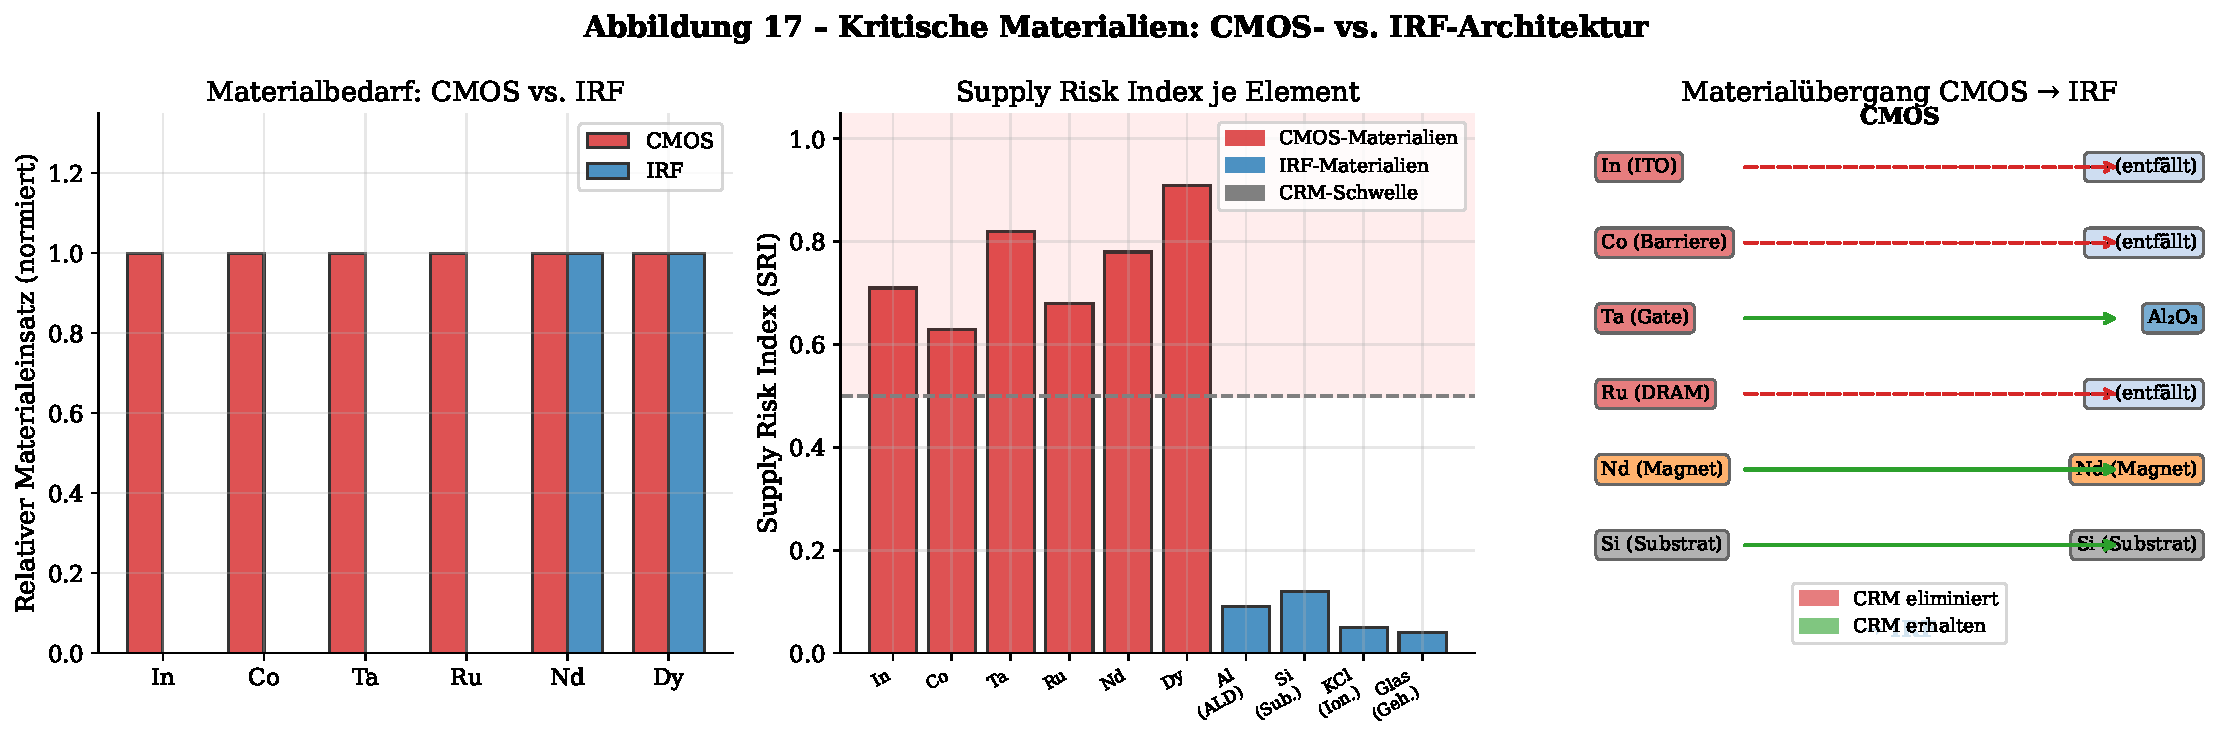
\includegraphics[width=\textwidth]{plots/plot17_irf_material.pdf}
  \caption{%
    \textbf{Kritische Materialien im PMSM-Antriebssystem: CMOS vs.~IRF.}
    \textit{Links:} Gruppiertes Balkendiagramm des spezifischen kritischen
    Materialanteils je Element (In, Co, Ta, Ru, Nd, Dy) für CMOS- und
    IRF-Implementierung. IRF-Werte für In, Co, Ta und Ru sind null (nicht
    benötigt), während Nd/Dy dem Magnetkreis zugeordnet bleiben.
    \textit{Mitte:} Supply Risk Index (SRI) je Element nach EU-CRM-Methodik
    2023; Schwelle CRM-gelistet/nicht-gelistet als horizontale Linie.
    Die IRF-Materialmenge hat keinen Beitrag oberhalb der CRM-Schwelle.
    \textit{Rechts:} Sankey-ähnliches Übergangsbild: Materialflüsse
    CMOS-Architektur (links) $\to$ IRF-Architektur (rechts), die
    wegfallenden kritischen Pfade (In, Co, Ta, Ru) als rot gestrichelte,
    die verbleibenden (Si, Al, KCl) als grüne Pfeile dargestellt.
  }
  \label{fig:irf_material}
\end{figure}

% ------------------------------------------------------------------
\section{Optik, Elektronik und Kommunikation}
\label{ssec:re_optik}
% ------------------------------------------------------------------

\subsection{Europium und Terbium: Reine Farben in Displays und Sicherheitsdruck}

Lanthanoidphosphore erzeugen durch die scharfen, aus $4f$-$4f$-Übergängen
stammenden Emissionslinien färberisch reinere Lichtemissionen als jede
andere Materialkategorie. Der Grund sind die von der $(5s)^2(5p)^6$-Schale
abgeschirmten $4f$-Elektronen: Kristallfelder verschieben die
Energieniveaus nur minimal, sodass die Emission nahezu monochromatisch bleibt.
\begin{itemize}
  \item \textbf{Eu$^{3+}$} (Rot, $\lambda \approx 612\,\text{nm}$) in Y$_2$O$_3$:Eu
        oder YVO$_4$:Eu -- Standard-Rotphosphor in Energiesparlampen und weißen
        LEDs.
  \item \textbf{Tb$^{3+}$} (Grün, $\lambda \approx 543\,\text{nm}$) in
        LaPO$_4$:Tb -- Standardgrünphosphor; wird ferner für
        Banknoten-Sicherheitsdrucke (UV-Lumineszenz) eingesetzt.
  \item \textbf{Eu$^{2+}$} (Blau, $\lambda \approx 460\,\text{nm}$, vibronisch
        verbreitert) in (Ba,Sr)MgAl$_{10}$O$_{17}$:Eu -- Blauphosphor in
        weißen pc-LEDs und CCFL-Hintergrundbeleuchtungen.
\end{itemize}
Ohne diese drei Phosphore wäre eine Herstellung von Weißlicht-LEDs mit
Farbwiedergabeindex $R_a > 90$ technisch nicht möglich.

\subsection{Erbium: Herzstück der optischen Fern\-kommunikation}

Erbium-dotierte Faserverstärker (EDFA, Erbium-Doped Fiber Amplifier) sind
seit Anfang der 1990er Jahre das unersetzliche Glied aller transozeansichen
Glasfaserkabel. Erbium-Ionen in einer Silikatfaser, gepumpt mit einem
$\SI{980}{\nano\metre}$-Diodenlaser, erzeugen stimulierte Emission im
C-Band ($1530$--$1565\,\text{nm}$) -- dem Spektralbereich minimaler
Faserabsorption. Eine einzige EDFA-Stufe legt optische Verstärkungen von
$\geq 30\,\text{dB}$ vor; alle transatlantischen Kabel nutzen sie in
Abständen von $\approx \SI{80}{\kilo\metre}$. Ohne Er gäbe es kein globales
Internet der heutigen Bandbreite.

% ------------------------------------------------------------------
\section{Globale Verfügbarkeit: Die Erde ist reich genug}
\label{ssec:re_global}
% ------------------------------------------------------------------

Die häufig zitierte Aussage, Seltene Erden seien nur in China verfügbar, ist
\emph{falsch}. Sie ist eine historische Konsequenz der Industriepolitik, keine
geologische Realität~\cite{alonso2012}. Abbildung~\ref{fig:re_reserven} zeigt
die Verteilung der \emph{bekannten Reserven} (USGS 2024) und die davon
fundamental abweichende Verteilung der \emph{aktuellen Produktion}.

\begin{figure}[htbp]
\centering
\begin{tikzpicture}[
  every node/.style={font=\footnotesize},
  >=Stealth,
]
%── Balkendiagramm: Reserven (links) vs. Produktion (rechts) ─────────────────
% Daten: Land / Reserven-% / Produktions-%
% Quelle: USGS 2024, gerundet
\def\barh{0.52}
\def\gap{0.72}

% Reserven-Balken (LINKS, wachsen nach links von x=0)
% Produktion-Balken (RECHTS, wachsen nach rechts von x=0)
% Skalierung: 1% → 0.115cm (Reserven max 35%, Prod max 60%)

% Hintergrundstreifen
\foreach \i in {0,1,2,3,4,5,6}{
  \ifodd\i \fill[gray!8] (-6.5, \i*\gap-0.1) rectangle (6.5, \i*\gap+\barh+0.1); \fi
}

% Achsenbeschriftung oben
\node[font=\footnotesize\bfseries, mainblue]  at (-3.2, 7.2) {Reserven [\%]};
\node[font=\footnotesize\bfseries, accentred] at ( 3.2, 7.2) {Produktion [\%]};
\draw[thick] (0, -0.4) -- (0, 7.0);
\draw[thick] (-6.5, -0.4) -- (6.5, -0.4);

% Gitterlinien
\foreach \v in {10,20,30,40,50,60}{
  \draw[gray!30] ( \v*0.095,  -0.4) -- ( \v*0.095,  7.0);
  \draw[gray!30] (-\v*0.115,  -0.4) -- (-\v*0.115,  7.0);
  \node[gray!60, font=\tiny, below] at ( \v*0.095,  -0.4) {\v};
  \node[gray!60, font=\tiny, below] at (-\v*0.115,  -0.4) {\v};
}

% Daten: Land / Reserven / Produktion / y-position
\foreach \land/\res/\prod/\yi in {
  China/35/60/0,
  Vietnam/18/10/1,
  Brasilien/17/2/2,
  Russland/10/8/3,
  Indien/6/4/4,
  Australien/5/7/5,
  {USA\,+\,Kanada}/4/5/6}{
  % Reserven-Balken (blau, links)
  \fill[mainblue!60] (-\res*0.115, \yi*\gap)
    rectangle (0, \yi*\gap+\barh);
  \node[right, mainblue!80, font=\scriptsize]
    at (-\res*0.115-0.05, \yi*\gap+\barh/2) {\res\,\%};
  % Produktion-Balken (rot, rechts)
  \fill[accentred!60] (0, \yi*\gap)
    rectangle (\prod*0.095, \yi*\gap+\barh);
  \node[left, accentred!80, font=\scriptsize]
    at (\prod*0.095+0.05, \yi*\gap+\barh/2) {\prod\,\%};
  % Land-Label (Mitte)
  \node[font=\scriptsize\bfseries, align=center]
    at (0, \yi*\gap + \barh + 0.1) {};
  \node[font=\scriptsize] at (0, \yi*\gap + \barh*0.5)
    {\textbf{\land}};
}

% Hervorhebung China-Asymmetrie
\draw[accentred, very thick, <->]
  (0, -0.9) -- (60*0.095, -0.9);
\draw[mainblue, very thick, <->]
  (-35*0.115, -0.9) -- (0, -0.9);
\node[accentred, font=\scriptsize, below] at (60*0.095/2, -1.1)
  {60\,\% Produktion};
\node[mainblue, font=\scriptsize, below] at (-35*0.115/2, -1.1)
  {35\,\% Reserven};

% Asterisk-Hinweis
\node[font=\scriptsize, gray, align=center] at (0, -1.8)
  {China: 35\,\% der Reserven, aber 60\,\% der Weltproduktion};
\end{tikzpicture}
\caption{Globale Verteilung der SE-Reserven (blau, links) versus SE-Produktion
  (rot, rechts) nach Ländern. Die fundamentale Asymmetrie ist offensichtlich:
  China hält $35\,\%$ der bekannten Reserven, produziert aber $60\,\%$ des
  globalen Angebots. Vietnam, Brasilien und Russland besitzen zusammen
  $45\,\%$ der Reserven, liefern aber nur $20\,\%$ der Produktion. Dies
  belegt, dass die Knappheit kein geologisches, sondern ein
  industriepolitisches Problem ist~\cite{usgs2024,massari2013}.}
\label{fig:re_reserven}
\end{figure}

Neben den etablierten Produzenten liegen bedeutende neue Lagerstätten bereit:
\begin{itemize}
  \item \textbf{Per Geijer (Schweden, LKAB):} Im Januar 2023 als größtes
        bekanntes SE-Depot Europas identifiziert, mit $>1\,\text{Mt}$ SE-Oxidäquivalenten
        (REO)~\cite{lkab2023}; Genehmigungsverfahren läuft.
  \item \textbf{Grönland (Kvanefjeld/Tanbreez):} Eines der weltweit größten
        primären SE-Vorkommen, gekoppelt mit Uran; politisch kontrovers.
  \item \textbf{Brasilien (Serra Amarela, Catalão):} Karbonatit-gebundene
        SE-Anreicherungen mit geringen Ce/La-Verhältnissen; Carbonatit-Bergbau
        seit 1976.
  \item \textbf{Vietnam (Yen Phu, Nam Xe):} Ionenabsorptions-Tone, ähnlich
        dem chinesischen ``Southern REE''-Typ; sehr schwerseltenerd-reiche
        Zusammensetzung.
  \item \textbf{Tiefsee-Sedimente (Pacific, IOZ):} Kobalt-reiche Krusten und
        polymetallische Knollen enthalten erhebliche SE-Gehalte
        ($>\SI{2000}{ppm}$); noch nicht kommerziell abgebaut.
  \item \textbf{Asteroidenbergbau (Zukunft):} Erdnahe Objekte (NEA) wie die
        Klasse der S- und C-Typ-Asteroiden enthalten lanthanoidreiche
        Chondrite. Programme wie AstroForge (USA) und Planetary Resources
        untersuchen deren langfristiges Potenzial~\cite{iea2024}.
\end{itemize}

% ------------------------------------------------------------------
\section{Kosmischer Ursprung -- der r-Prozess in Supernovae und
            Neutronensternverschmelzungen}
\label{ssec:re_kosmos}
% ------------------------------------------------------------------

Seltene Erden entstehen auf kosmischer Skala im sogenannten
\emph{r-Prozess} (\emph{rapid neutron capture process}): dem schnellen,
sukzessiven Einfang von Neutronen durch Saatkerne (typisch $^{56}$Fe) in
einer Umgebung, in der die Neutronendichte derart hoch ist
($n_n \gtrsim 10^{20}\,\text{cm}^{-3}$), dass Neutroneneinfang schneller
abläuft als $\beta^-$-Zerfall. Nach dem bahnbrechenden
$B^2FH$-Aufsatz~\cite{burbidge1957} wurden als astrophysikalische
Stätten hauptsächlich die Umhüllungsregionen von Kern-Kollaps-Supernovae
(SN~II) diskutiert. Seit der Beobachtung des Kilonova-Ereignisses GW170817
(August 2017)~\cite{abbott2016} gilt es als gesichert, dass
Neutronensternverschmelzungen der dominante r-Prozess-Schauplatz sind:
Spektroskopische Identifikation von Strontium (Sr, $Z = 38$) und Barium
(Ba, $Z = 56$) im Kilonova-Spektrum belegt die r-Prozess-Nukleosynthese
direkt~\cite{smartt2017}.

\begin{sidewaysfigure}
\centering
\resizebox{!}{0.6\textwidth}{%
\begin{tikzpicture}[
  >=Stealth,
  thick,
  every node/.style={font=\scriptsize},
]
%── Achsen (Nuklid-Chart-Ausschnitt: N horizontal, Z vertikal) ──────────────
\def\cellsize{0.48}
\def\Nmin{20} \def\Nmax{54}
\def\Zmin{22} \def\Zmax{62}

\draw[->] (0,0) --
  ({(\Nmax-\Nmin+2)*\cellsize}, 0)
  node[right, font=\small] {Neutronenzahl $N$};
\draw[->] (0,0) --
  (0, {(\Zmax-\Zmin+2)*\cellsize})
  node[above, font=\small] {Protonenzahl $Z$};

% Achsenbeschrif\-tungen
\foreach \Nval/\Ntick in {20/20,28/28,40/40,50/50}{
  \node[below, gray] at ({(\Nval-\Nmin)*\cellsize}, -0.1)
    {\Nval};
  \draw[gray!40] ({(\Nval-\Nmin)*\cellsize}, 0) --
    ({(\Nval-\Nmin)*\cellsize}, {(\Zmax-\Zmin+1)*\cellsize});
}
\foreach \Zval/\sym in {26/Fe,36/Kr,50/Sn,60/Nd}{
  \node[left, gray] at (-0.1, {(\Zval-\Zmin)*\cellsize})
    {$Z\!=\!\Zval$ (\sym)};
  \draw[gray!40] (0, {(\Zval-\Zmin)*\cellsize}) --
    ({(\Nmax-\Nmin+1)*\cellsize},{(\Zval-\Zmin)*\cellsize});
}

%── Stabilitätstal: vereinfacht als diagonale Linie ──────────────────────────
% Für A = Z+N, stabiele Kerne: N ≈ Z für kleine A, N ≈ 1.4Z für große A
% Approximation: N_stable ≈ Z + (Z-20)*0.08  für Z>20
\draw[black, very thick] plot[smooth] coordinates {
  ({(26-\Nmin)*0.48}, {(26-\Zmin)*0.48})
  ({(31-\Nmin)*0.48}, {(28-\Zmin)*0.48})
  ({(36-\Nmin)*0.48}, {(30-\Zmin)*0.48})
  ({(40-\Nmin)*0.48}, {(32-\Zmin)*0.48})
  ({(44-\Nmin)*0.48}, {(34-\Zmin)*0.48})
  ({(48-\Nmin)*0.48}, {(36-\Zmin)*0.48})
  ({(52-\Nmin)*0.48}, {(38-\Zmin)*0.48})
  ({(50-\Nmin)*0.48}, {(40-\Zmin)*0.48})
  ({(52-\Nmin)*0.48}, {(43-\Zmin)*0.48})
  ({(52-\Nmin)*0.48}, {(46-\Zmin)*0.48})
  ({(52-\Nmin)*0.48}, {(50-\Zmin)*0.48})
  ({(52-\Nmin)*0.48}, {(50-\Zmin)*0.48})
};
\node[right, font=\tiny, black] at ({(53-\Nmin)*0.48}, {(46-\Zmin)*0.48})
  {Stabilitätstal};

%── r-Prozess-Pfad: neutronenreich, unterhalb Stabilitätstal ──────────────
\draw[mainblue, very thick, dashed] plot[smooth] coordinates {
  ({(20-\Nmin)*0.48}, {(26-\Zmin)*0.48})
  ({(26-\Nmin)*0.48}, {(30-\Zmin)*0.48})
  ({(32-\Nmin)*0.48}, {(34-\Zmin)*0.48})
  ({(38-\Nmin)*0.48}, {(38-\Zmin)*0.48})
  ({(44-\Nmin)*0.48}, {(42-\Zmin)*0.48})
  ({(50-\Nmin)*0.48}, {(46-\Zmin)*0.48})
  ({(54-\Nmin)*0.48}, {(50-\Zmin)*0.48})
};
\node[mainblue, font=\tiny, align=center] at ({(40-\Nmin)*0.48}, {(36-\Zmin)*0.48-0.4})
  {r-Prozess-Pfad};

%── Beta-minus-Zerfall Pfeile (r-Prozess → Stabilitätstal) ──────────────────
\foreach \Nx/\Zx in {32/31, 38/36, 44/41, 50/46}{
  \draw[->, accentred, thick]
    ({(\Nx-\Nmin)*0.48}, {(\Zx-0.5-\Zmin)*0.48}) --
    ({(\Nx-1-\Nmin)*0.48}, {(\Zx+0.5-\Zmin)*0.48});
}
\node[accentred, font=\tiny] at ({(36-\Nmin)*0.48+0.5}, {(34-\Zmin)*0.48+0.6})
  {$\beta^-$-Zerfall};

%── Neutroneneinfang-Pfeile ───────────────────────────────────────────────────
\foreach \Nx/\Zx in {22/27, 28/31, 34/35}{
  \draw[->, darkgreen, thick]
    ({(\Nx-\Nmin)*0.48}, {(\Zx-\Zmin)*0.48+0.15}) --
    ({(\Nx+2-\Nmin)*0.48}, {(\Zx-\Zmin)*0.48+0.15});
}
\node[darkgreen, font=\tiny] at ({(27-\Nmin)*0.48}, {(29-\Zmin)*0.48+0.4})
  {$(n,\gamma)$-Einfang};

%── Lanthanid-Region schattiert ───────────────────────────────────────────────
\begin{scope}[on background layer]
  \fill[accentred!15, rounded corners=4pt]
    ({(44-\Nmin)*0.48-0.2}, {(57-\Zmin)*0.48-0.2}) rectangle
    ({(54-\Nmin)*0.48+0.2}, {(62-\Zmin)*0.48+0.2});
\end{scope}
\node[accentred, font=\tiny\bfseries, align=center] at ({(49-\Nmin)*0.48}, {(60-\Zmin)*0.48})
  {Lanthanide\\(r-Prozess-\\Produkte)};

%── Seed-Kern Fe markieren ────────────────────────────────────────────────────
\fill[black] ({(30-\Nmin)*0.48},{(26-\Zmin)*0.48}) circle (3pt);
\node[below right, font=\tiny] at ({(30-\Nmin)*0.48},{(26-\Zmin)*0.48})
  {$^{56}$Fe (Saatkern)};

%── Kilonova-Annotation ────────────────────────────────────────────────────────
\node[draw, rounded corners=3pt, fill=yellow!20, font=\scriptsize,
      inner sep=4pt, align=center] at ({(50-\Nmin)*0.48+1.5}, 0.5)
  {GW170817 (2017):\\Sr, Ba detektiert};
\draw[->, thin, gray] ({(50-\Nmin)*0.48+0.5}, 0.8) to[bend left=15]
  ({(50-\Nmin)*0.48},{(38-\Zmin)*0.48+0.1});

\end{tikzpicture}%
}%
\caption{Vereinfachter Ausschnitt aus dem Nukliddiagramm ($N$-$Z$-Ebene)
  zur Illustration des r-Prozesses.}
\label{fig:re_rprocess}
\end{sidewaysfigure}

Abbildung \ref{fig:re_rprocess} zeigt den vereinfachten Ausschnitt aus dem Nukliddiagramm. \textbf{Schwarz:} Stabilitätstal der $\beta$-stabilen Kerne.
\textbf{Blau gestrichelt:} r-Prozess-Pfad -- tief im neutronenreichen
Bereich; hier wird durch schnellen Neutroneneinfang ($n, \gamma$, grüne
Pfeile) die Massenzahl aufgebaut.
\textbf{Rot:} $\beta^-$-Zerfälle, die den r-Prozess-Pfad schrittweise
zurück zum Stabilitätstal führen, sobald der Neutronenfluss nachlässt.
Das neutronenreiche Endsystem ``wartet'' bei magischen Neutronenzahlen
($N = 50, 82, 126$). \textbf{Rosa Box:} Lanthanid-Region ($Z = 57$--$71$) --
alle Seltenen Erden sind primäre r-Prozess-Produkte.
Das Kilonova-Ereignis \textbf{GW170817} lieferte 2017 den direkten
experimentellen Nachweis, dass Neutronensternverschmelzungen der
dominante r-Prozess-Schauplatz sind~\cite{abbott2016,smartt2017}.

Die Konsequenz für die Ressourcenperspektive ist fundamental: Seltene Erden
sind keine kosmische Seltenheit. Sie entstehen in jedem Neutronenstern-Event
und akkumulieren in allen metallischen Festkörpern des Sonnensystems -- in
der Erdkruste, in Meteoriten und potentiell abbaubar in Asteroiden. Die
Beschränkung auf irdische, geopolitisch zugängliche Quellen ist eine
\emph{gewählte} Beschränkung, keine physikalisch erzwungene.

% ------------------------------------------------------------------
\section{Recycling und Kreislaufwirtschaft}
\label{ssec:re_recycling}
% ------------------------------------------------------------------

Die globale Recyclingrate für Seltene Erden liegt derzeit bei $< 1\,\%$~\cite{weng2015}
-- ein eklatantes technologisches und wirtschaftspolitisches Versagen angesichts
des Versorgungsrisikos. Das Recyclingpotential ist enorm:
\begin{itemize}
  \item Jährlich werden weltweit $>12\,\text{Millionen}$ Elektro- und
        Hybridfahrzeuge ausgemustert, jedes enthält $1$--$3\,\text{kg}$ Nd.
  \item $>30\,\text{GW}$ Windturbinenkapazität werden bis 2030 jährlich als
        Altbestand anfallen, mit je $200$--$600\,\text{kg}$ NdFeB.
  \item Festplatten, Lautsprecher, MRT-Magnete: Hunderte von Tonnen pro Jahr.
\end{itemize}

Das in Abschnitt~\ref{ssec:ausblick_synergie} beschriebene
Hydrogen-Decrepitation-Verfahren ist die technologisch ausgereifteste
Methode. Ergänzend werden entwickelt:
\begin{enumerate}[label=\arabic*.]
  \item \textbf{Selektive ionische Flüssigkeits-Extraktion (SILX):} Maßgeschneiderte
        ionische Flüssigkeiten separieren SE$^{3+}$-Ionen aus Laugungslösungen
        mit Trennfaktoren $>100$, die klassische Solvent-Extraktion (D2EHPA)
        nur selten überschreitet.
  \item \textbf{Molten-Salt-Elektrolyse (Direktrecycling):} Altmagneten werden
        in KF/LiF-Schmelze (T $\approx\SI{750}{\celsius}$) aufgeschlossen;
        Nd und Dy werden gemeinsam elektrochemisch abgeschieden und als
        gemischtes Metall direkt für neue Magnete eingesetzt.
  \item \textbf{Kurzkreislauf-Sinterung (Urban Mining $\to$ Magnet):}
        Das geschredderte und klassierte Altmagnetpulver wird ohne
        vollständige Metallurgie direkt zu neuen gesinterten Magneten
        verarbeitet (``magnet-to-magnet''); Verluste $< 5\,\%$ von
        $B_r$ nachgewiesen.
\end{enumerate}

Abbildung~\ref{fig:re_lieferkette} zeigt die vollständige SE-Lieferkette
mit Engpass und möglichen Recycling-Bypässen.

\begin{sidewaysfigure}[htbp]
\centering
\begin{tikzpicture}[
  >=Stealth,
  thick,
  every node/.style={font=\footnotesize},
  box/.style={draw, rounded corners=5pt, minimum width=2.2cm,
              minimum height=0.9cm, align=center, inner sep=4pt},
  bottle/.style={box, fill=accentred!30, draw=accentred!80},
  normal/.style={box, fill=mainblue!15, draw=mainblue!60},
  green/.style={box, fill=darkgreen!20, draw=darkgreen!70},
]
%── Hauptkette (horizontal) ──────────────────────────────────────────────────
\def\xsp{3.0}
\node[normal] (mine)   at (0*\xsp, 0)  {Bergbau\\(Mining)};
\node[bottle] (sep)    at (1*\xsp, 0)  {Separation};
\node[normal] (alloy)  at (2*\xsp, 0)  {Legierung\\(Alloying)};
\node[normal] (comp)   at (3*\xsp, 0)  {Bauteil\\(Component)};
\node[normal] (prod)   at (4*\xsp, 0)  {Produkt\\(Product)};
\node[normal] (use)    at (5*\xsp, 0)  {Nutzung\\(End-of-Life)};

%── Pfeile Hauptkette ─────────────────────────────────────────────────────────
\foreach \from/\to in {mine/sep, sep/alloy, alloy/comp, comp/prod, prod/use}{
  \draw[->] (\from) -- (\to);
}

%── Recycling-Bypass (unten) ─────────────────────────────────────────────────
\node[green] (recyc) at (2.5*\xsp, -2.0) {Recycling\\(HD, SILX,\\Molten Salt)};
\draw[->, darkgreen, thick, bend right=20] (use)   to (recyc);
\draw[->, darkgreen, thick, bend right=20] (recyc) to (alloy);

%── Bypass-Pfeil: Direktrecycling Magnet → Magnet ────────────────────────────
\draw[->, darkgreen!80, dashed, thick, bend right=12]
  (use) to node[below, font=\tiny, darkgreen] {Magnet-to-Magnet} (comp);

%── Alternativen-Pfeil ─────────────────────────────────────────────────────────
\node[draw, dashed, fill=orange!15, rounded corners=4pt,
      font=\scriptsize, inner sep=4pt, align=center]
  (alt) at (2*\xsp, 2.0) {SE-freie\\Alternativen\\(Fe$_{16}$N$_2$, MnBi)};
\draw[->, orange!80, dashed, thick] (alt) to (comp);

%── Geopolitik-Pfeil ─────────────────────────────────────────────────────────

%── Legende ───────────────────────────────────────────────────────────────────
\node[normal, minimum width=1.6cm, font=\scriptsize] at (0, -3.2)  {normal};
\node[bottle, minimum width=1.6cm, font=\scriptsize] at (2, -3.2)  {Engpass};
\node[green,  minimum width=1.6cm, font=\scriptsize] at (4, -3.2)  {Recycling};
%\node[draw=orange, fill=orange!15, rounded corners=4pt,
%      minimum width=1.6cm, font=\scriptsize, inner sep=3pt]
%  at (6*\xsp*0.55+0.3, -3.2) {Alternative};
\end{tikzpicture}
\caption{SE-Lieferkette von der Abbaulokalität bis zum Endprodukt und zurück.
  Der rote Engpass liegt bei der \textbf{Separation} (hydro-metallurgische
  Trennung der SE-Elemente voneinander): Hier liegen $>90\,\%$ der weltweiten
  Kapazität in China. Grüne Pfeile zeigen die Recycling-Rückführung
  (Hydrogen-Decrepitation, ionische Flüssigkeiten, Molten-Salt-Elektrolyse)
  zurück in die Legierungsstufe; der gestrichelte grüne Pfeil zeigt den
  direkten Magnet-to-Magnet-Recyclingpfad. Orangefarbener Kasten: SE-freie
  Alternativen können den Magnete-Bauteil-Pfad ergänzen oder teilweise
  ersetzen.}
\label{fig:re_lieferkette}
\end{sidewaysfigure}

% ------------------------------------------------------------------
\section{Geopolitische Dimension und politischer Handlungsbedarf}
\label{ssec:re_geopolitik}
% ------------------------------------------------------------------

Das Marktmonopol der Seltenen Erden ist ein Paradebeispiel für industrielle
Abhängigkeiten, die aus der Kombination von Ressourcenvorteil, gezielter
Subventionspolitik und externer Passivität entstehen. China kann durch
Exportquoten oder -steuern -- wie geschehen 2010--2014 -- die Weltmarktpreise
für Dy oder Tb kurzfristig um $>1000\,\%$ treiben und damit die globale
Rohstoffversorgung für Elektromotoren, Windturbinen und Militärtechnik
empfindlich stören~\cite{massari2013}.

Die institutionellen Antworten wurden formuliert:
\begin{itemize}
  \item \textbf{EU Critical Raw Materials Act (2024):} Verpflichtendes
        Diversifizierungsziel: bis 2030 müssen $40\,\%$ der EU-Jahresbedarfs
        an Seltenen Erden aus heimischer Förderung und $15\,\%$ aus Recycling
        stammen; kein Drittland darf $>65\,\%$ des EU-Bedarfs im strategischen
        Segment decken~\cite{eu2023}.
  \item \textbf{US Inflation Reduction Act / Critical Minerals Initiative:}
        Steuerliche Anreize für Batterien und Magnete aus US-freundlichen
        Quellen; Förderung heimischer Recyclinganlagen.
  \item \textbf{Minerals Security Partnership (MSP, 2022):} G7-Initiative
        zum Aufbau resilienter Rohstofflieferketten; umfasst 14 Länder
        und Investitionsgarantien für Lagerstättenentwicklung.
  \item \textbf{Japan's JOGMEC:} Japan hat nach der Exportkrise 2010 als
        erste große Industrienation eine staatlich koordinierte
        SE-Diversifizierungsstrategie umgesetzt: Investitionen in
        australische, kasachische und indische Abbau- und
        Verarbeitungsprojekte.
\end{itemize}

Der politische Wille ist damit erkennbar gestiegen. Es fehlt jedoch noch an
Geschwindigkeit und Skalierung: Vom Explorationsnachweis bis zur
Produktionsaufnahme einer neuen Lagerstätte vergehen typischerweise
$10$--$20\,\text{Jahre}$ (Genehmigungsverfahren, Infrastruktur,
Verarbeitungsanlage). Recycling und Substitution sind die kurzfristig
wirksameren Hebel.

\begin{hinweis}[Zusammenfassung: Seltene Erden -- Befunde und Handlungsfelder]
  Die sieben wichtigsten Erkenntnisse dieses Kapitels:
  \begin{enumerate}[label=\arabic*., noitemsep]
    \item Seltene Erden sind \emph{nicht geologisch selten}, sondern diffus
          verteilt und schwer konzentrierbar.
    \item China hält das Monopol durch \emph{Industriepolitik}, nicht durch
          Geologie -- die Reserven verteilen sich auf sechs Kontinente.
    \item Medizinisch sind Gd (MRT) und Lu-177 (PRRT) unmittelbar
          lebensrettend, Ho/Er/Tm für chirurgische Laser unverzichtbar.
    \item Nd und Dy sind das physikalische Rückgrat der Energiewende
          (NdFeB-Magnete für Wind, BEV, Servomotoren).
    \item Alle Seltenen Erden entstammen dem r-Prozess in
          Neutronensternverschmelzungen -- kosmisch gesehen ist die
          Verfügbarkeit unbegrenzt.
    \item Die globale Recyclingrate von $<1\,\%$ ist technisch und
          wirtschaftlich vollständig lösbar; HD-Verfahren und
          Magnet-to-Magnet-Recycling sind industriereif.
    \item SE-freie Alternativen (Fe$_{16}$N$_2$, MnBi, L1$_0$-FeNi) können
          mittelfristig für Niedrig-Leistungsapplikationen NdFeB ersetzen;
          für Hochleistungsanwendungen bleiben SE vorerst unverzichtbar.
  \end{enumerate}
\end{hinweis}

% ─────────────────────────────────────────────────────────────────────────────
\chapter{Legitime Anwendungen der Gravitationskraft}
\label{sec:legitim}
% ─────────────────────────────────────────────────────────────────────────────

\section{Gezeitenkraftwerke}

Gezeitenkraftwerke nutzen die periodische Gravitationswirkung von Mond und Sonne
auf die Meere. Die Gezeitenbeschleunigung auf der Erdoberfläche:

\begin{equation}
  a_{\text{tidal}} = \frac{2\G M_M R_E \cos\theta}{d_{\text{EM}}^3}
  \approx \SI{1.1e-6}{\metre\per\second\squared}
  \label{eq:gezeitenkraft}
\end{equation}

Bekannte Gezeitenkraftwerke:

\begin{table}[H]
  \centering
  \caption{Betriebliche Gezeitenkraftwerke weltweit}
  \label{tab:gezeiten}
  \begin{tabular}{lrrl}
    \toprule
    \textbf{Anlage} & \textbf{Leistung} & \textbf{Land} & \textbf{Jahr} \\
    \midrule
    La Rance (Gezeitenwehr) & \SI{240}{\mega\watt} & Frankreich & 1966 \\
    Sihwa-See              & \SI{254}{\mega\watt} & Südkorea   & 2011 \\
    Annapolis Royal        & \SI{20}{\mega\watt}  & Kanada     & 1984 \\
    \bottomrule
  \end{tabular}
\end{table}

\section{Pumpspeicherkraftwerke}

Pumpspeicher speichern \emph{elektrische} Energie als gravitative potentielle
Energie, indem sie bei Ãœberschussproduktion Wasser in ein Oberbecken pumpen:

\begin{equation}
  E_{\text{speicher}} = mg\Delta h \cdot \eta_{\text{pump}} \cdot \eta_{\text{turbine}}
  \approx mgh \cdot 0.75 \text{ bis } 0.85
  \label{eq:pumpspeicher}
\end{equation}

\section{Schwungradspeicher}

Ein Schwungrad speichert rotatorische kinetische Energie (nicht gravitativ, aber verwandt):
\begin{equation}
  E_{\text{Schwung}} = \frac{1}{2}I\omega^2 = \frac{1}{2}mr^2\omega^2
  \label{eq:schwungrad}
\end{equation}

Mit $m = \SI{100}{\kilogram}$, $r = \SI{0.5}{\metre}$, $\omega = \SI{1000}{\radian\per\second}$:
\begin{equation}
  E = \frac{1}{2} \cdot \SI{100}{} \cdot (\SI{0.5}{})^2 \cdot (\SI{1000}{})^2
  = \SI{12.5e6}{\joule} = \SI{3.47}{\kilo\watt\hour}
\end{equation}

\begin{figure}[H]
  \centering
  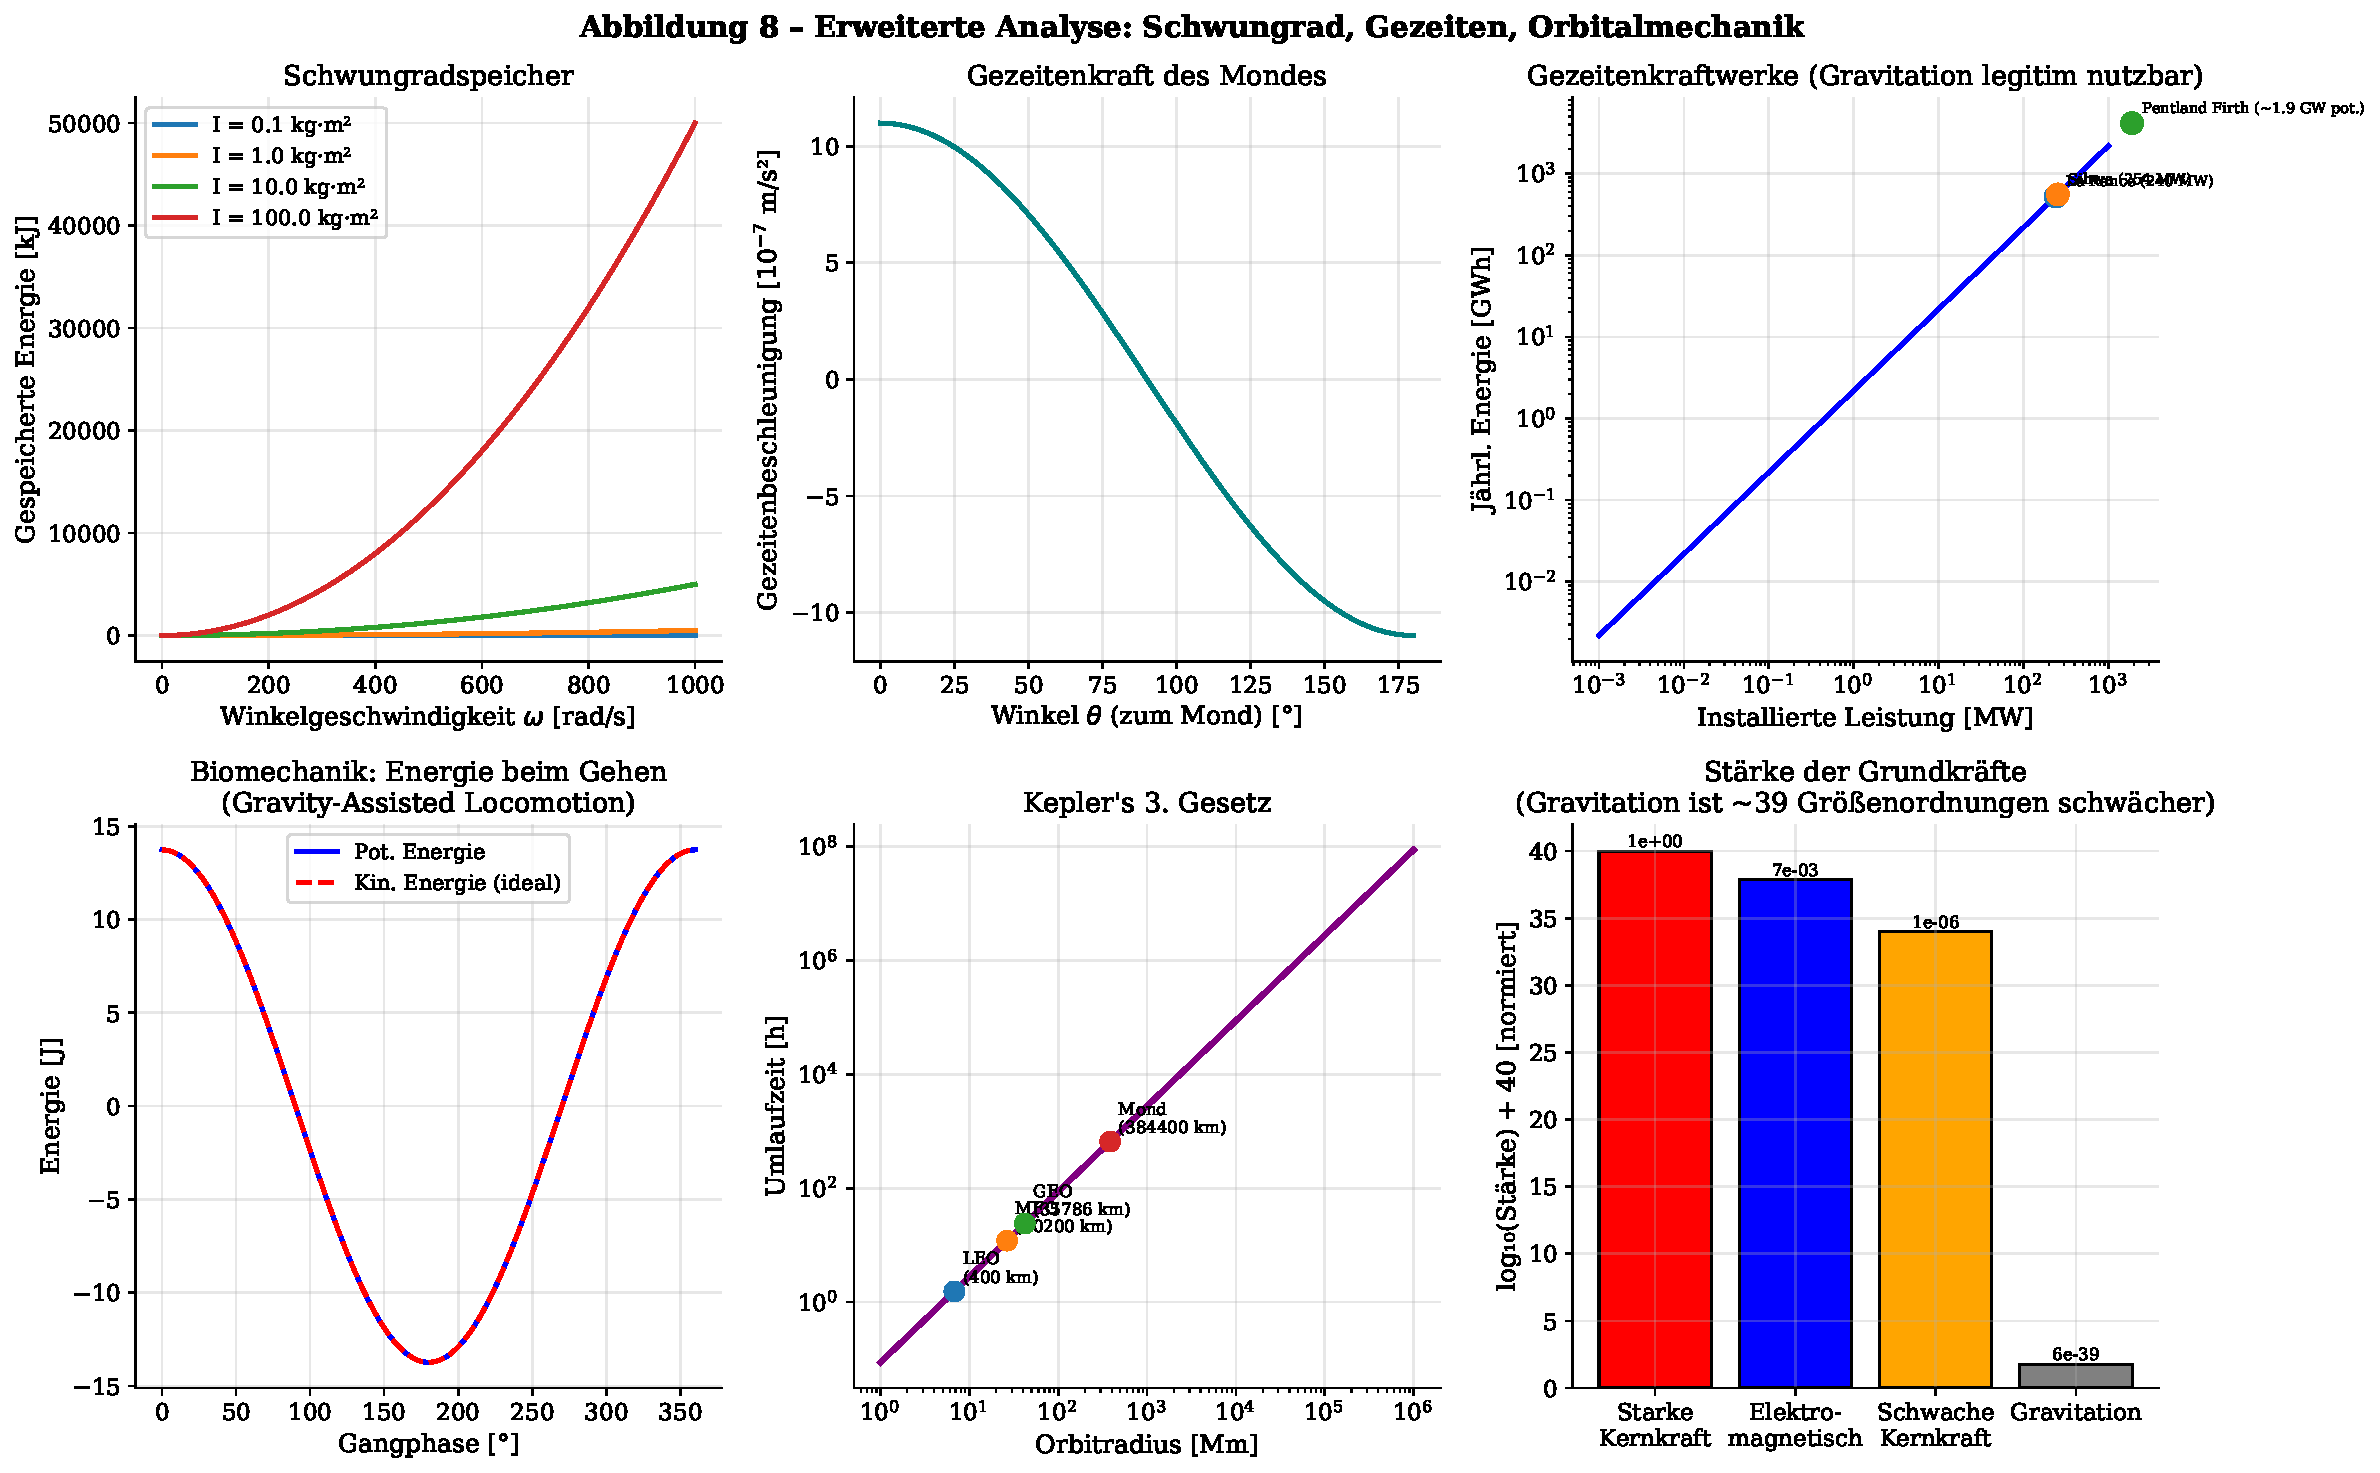
\includegraphics[width=\textwidth]{plots/plot8_erweitert.pdf}
  \caption{%
    \textbf{Legitime gravitative Anwendungen.}
    \textit{Oben links:} Schwungradspeicher -- gespeicherte Energie als Funktion
    der Winkelgeschwindigkeit für verschiedene Trägheitsmomente.
    \textit{Oben mitte:} Gezeitenbeschleunigung des Mondes auf der Erdoberfläche
    als Funktion des Winkels zum Mond.
    \textit{Oben rechts:} Jährliche Energieproduktion realer Gezeitenkraftwerke.
    \textit{Unten links:} Inverted-Pendulum-Modell des menschlichen Gangs:
    gravitative potentielle Energie wird in kinetische Energie umgewandelt.
    \textit{Unten mitte:} Kepler-Diagramm der Umlaufzeiten als Ausdruck des
    Gravitationsspeichers in der Orbitalmechanik.
    \textit{Unten rechts:} Stärkenvergleich der vier Grundkräfte -- die Schwerkraft
    ist $\sim 10^{39}$-mal schwächer als die Kernkraft.
  }
  \label{fig:legitim}
\end{figure}

% ─────────────────────────────────────────────────────────────────────────────
\chapter{Formale Zusammenfassung der Beweise}
\label{sec:beweise}
% ─────────────────────────────────────────────────────────────────────────────

\section{Haupttheoreme}

Wir fassen die fundamentalen Beweise zusammen:

\begin{theorem}[Unmöglichkeit des Gravitationsmotors als Perpetuum Mobile]
  \label{thm:hauptsatz}
  Es ist physikalisch unmöglich, eine Maschine zu konstruieren, die:
  \begin{enumerate}[leftmargin=2em, label=(\alph*)]
    \item ausschließlich durch die Gravitationskraft angetrieben wird,
    \item in einem geschlossenen Kreisprozess betrieben wird,
    \item dauerhaft nützliche mechanische Arbeit nach außen abgibt,
    \item ohne externe Energiezufuhr auskommt.
  \end{enumerate}
\end{theorem}

\begin{proof}
  Wir beweisen die Unmöglichkeit auf drei unabhängigen Wegen:

  \textbf{Beweis 1 -- Konservativität:}
  Da $\vek{F}_{\text{grav}} = -m\nabla\Phi$ ein konservatives Kraftfeld ist, gilt
  nach Satz~\ref{thm:konservativ}:
  \begin{equation}
    \oint_{\mathcal{C}} \vek{F}_{\text{grav}} \cdot \dd\vek{s} = 0
  \end{equation}
  Die Netto-Arbeit im Kreisprozess ist exakt null. Eine Maschine kann nur dann
  Netto-Arbeit \emph{ausgeben}, wenn sie Energie \emph{aufnimmt} -- was dem
  definierten ``Motor ohne externe Quelle'' widerspricht. $\square$

  \textbf{Beweis 2 -- Energieerhaltung (1. Hauptsatz):}
  Für ein abgeschlossenes mechanisches System gilt:
  \begin{equation}
    E_{\text{kin}} + E_{\text{pot}} + Q_{\text{Verluste}} = \text{const.}
  \end{equation}
  Im Kreisprozess kehren $E_{\text{kin}}$ und $E_{\text{pot}}$ zu ihren
  Ausgangswerten zurück. Die externen Verluste $Q > 0$ müssen aus einer
  Quelle stammen -- in einem geschlossenen System gibt es keine. $\square$

  \textbf{Beweis 3 -- Zweiter Hauptsatz (Entropie):}
  Jede reale Maschine erzeugt Entropie $\Delta S_{\text{irr}} > 0$. Diese
  Entropie entspricht der Degradation nutzbarer Energie. Im Laufe der Zeit
  tendiert jede reale Maschine zum thermodynamischen Gleichgewicht --
  sie kommt zum Stillstand. $\square$

  Da alle drei Beweise unabhängig sind und dasselbe Ergebnis liefern, ist
  die Unmöglichkeit dreifach gesichert.
\end{proof}

\section{Schranken für reale Systeme}

Für jeden realen Gravitationsmotor (mit Reibung) gilt:

\begin{align}
  \eta_{\text{real}} &= \frac{W_{\text{nutz}}}{W_{\text{grav,brutto}}} < 1 \label{eq:eta_real}\\
  W_{\text{nutz}} &= W_{\text{grav,brutto}} - W_{\text{Reibung}} - W_{\text{Rückhub}} \label{eq:nutzarbeit}\\
  &= mgh - Q_{\text{Reib}} - mgh = -Q_{\text{Reib}} \leq 0 \label{eq:nutzarbeit2}
\end{align}

Gleichung~\eqref{eq:nutzarbeit2} zeigt: Die Nutzarbeit ist \emph{negativ oder null} --
ein Gravitationsmotor kann keine nutzbare Arbeit liefern, er verbraucht sie sogar.

\begin{figure}[H]
  \centering
  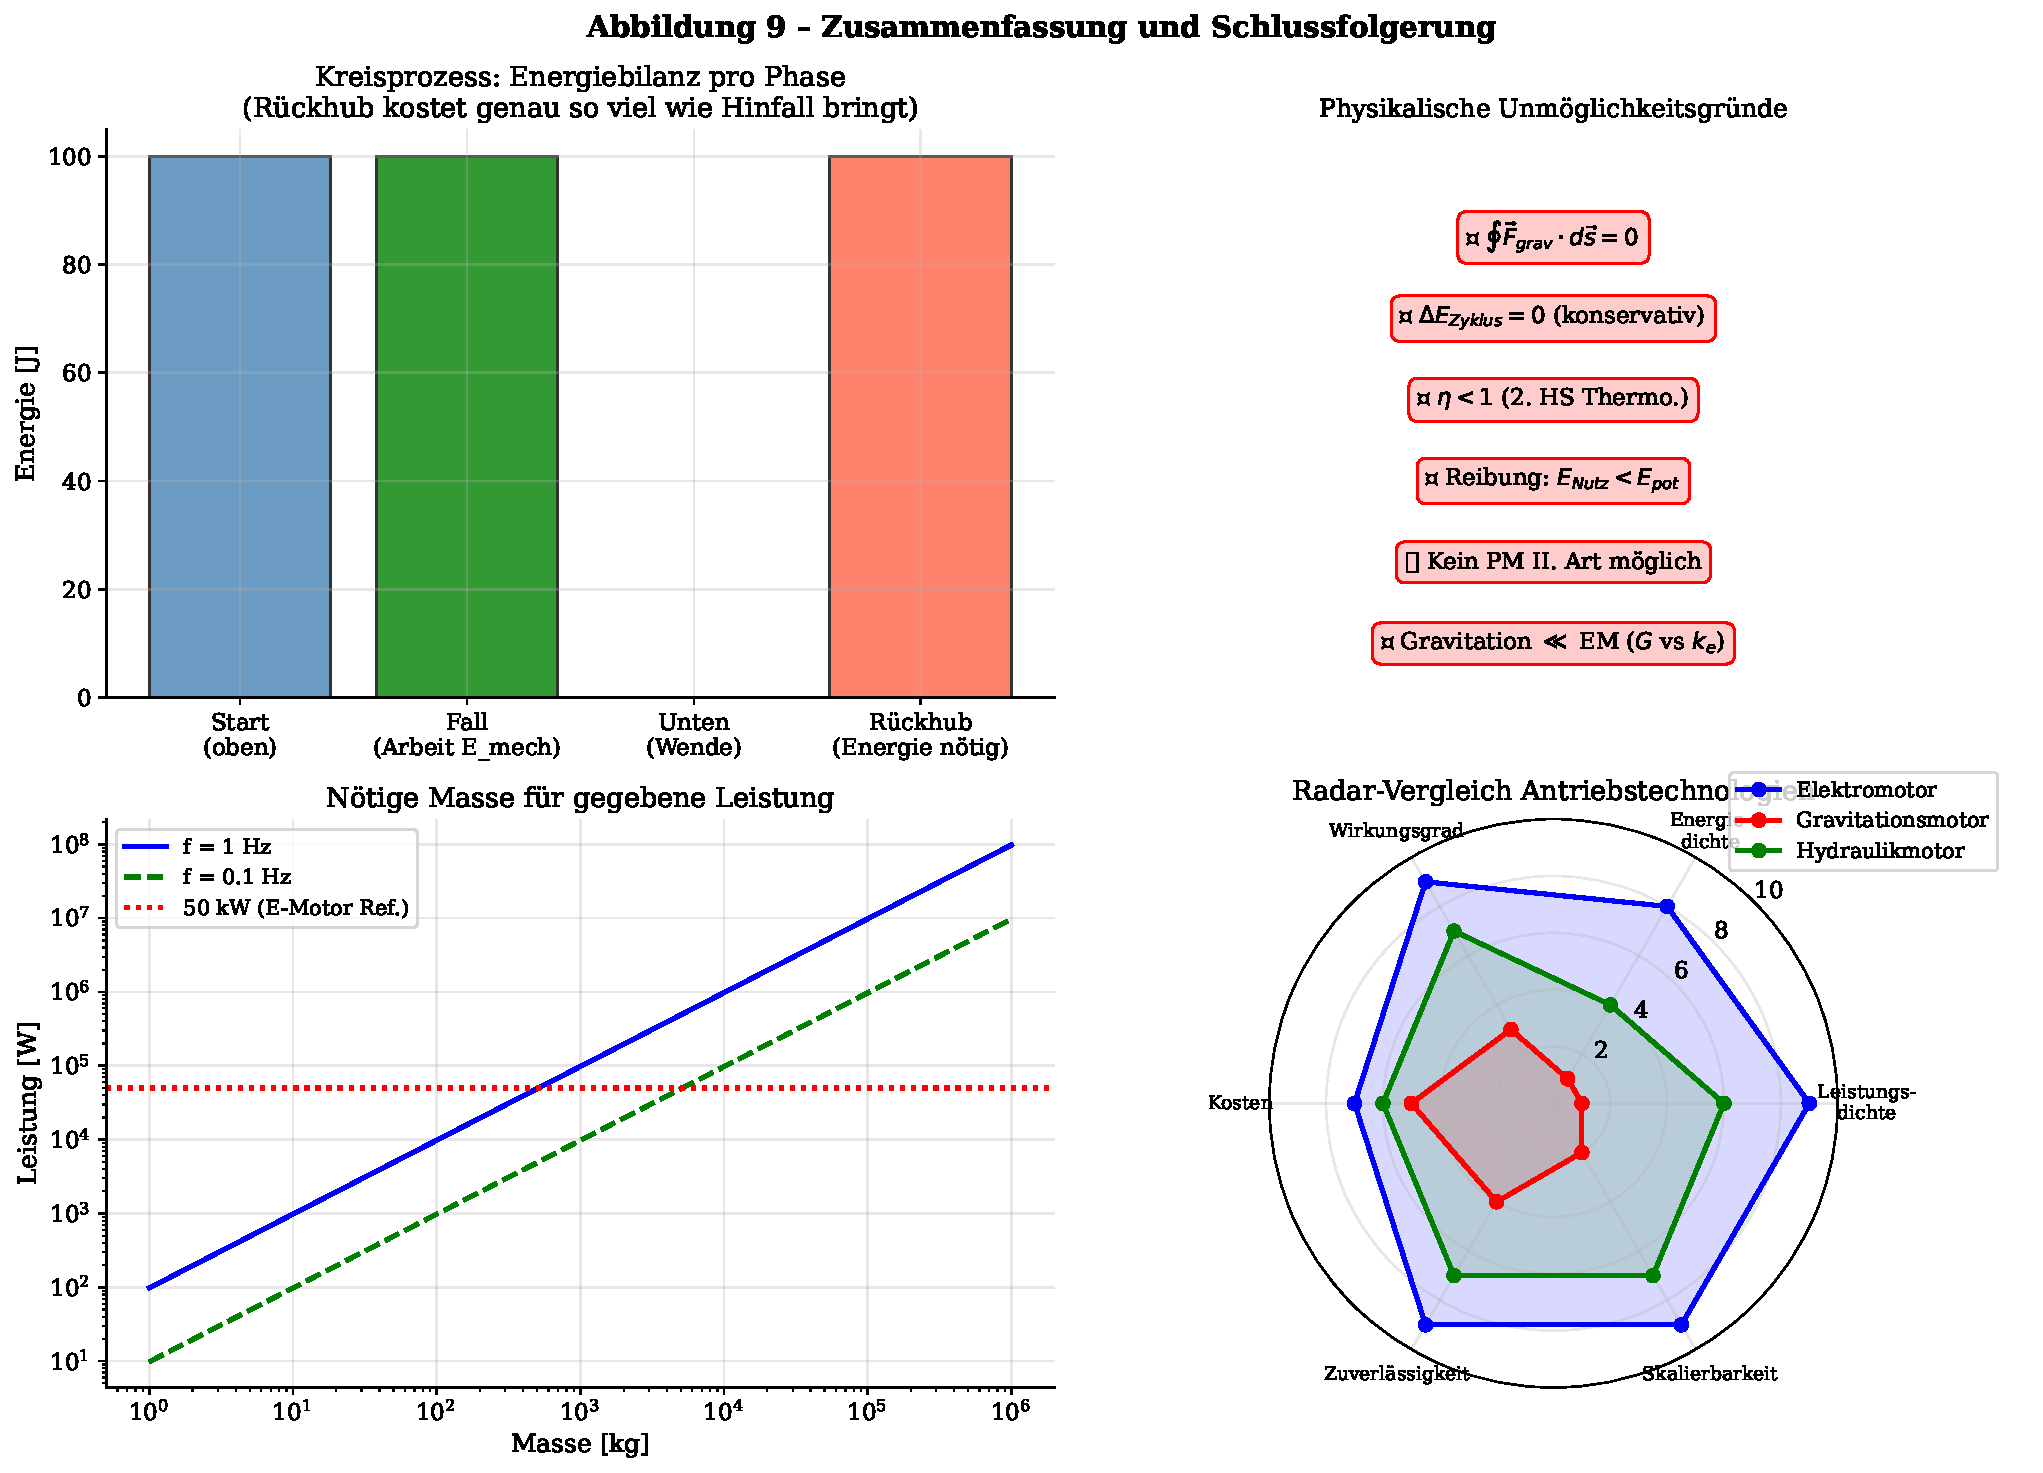
\includegraphics[width=\textwidth]{plots/plot9_zusammenfassung.pdf}
  \caption{%
    \textbf{Zusammenfassung der Analysen.}
    \textit{Oben links:} Kreisprozess-Energiebilanz: Die Phasen ``Fall'' (gewonnene
    Energie) und ``Rückhub'' (aufgewendete Energie) heben sich exakt auf.
    \textit{Oben rechts:} Übersicht der physikalischen Unmöglichkeitsgründe.
    \textit{Unten links:} Skalierungsanalyse: Die benötige Masse für eine gegebene
    Leistung -- um \SI{50}{\kilo\watt} zu erreichen, benötigt man $\approx
    \SI{510}{\kilogram}$ bei \SI{10}{\metre} Fallhöhe und \SI{1}{\second} Zyklus.
    Das bedeutet über \SI{500}{\kilogram} müssen jede Sekunde \SI{10}{\metre}
    angehoben werden -- wofür genau dieselbe Energie gebraucht wird.
    \textit{Unten rechts:} Radar-Vergleich der Antriebstechnologien. Der
    Gravitationsmotor schneidet in fast allen Kategorien schlechter ab als
    der Elektromotor.
  }
  \label{fig:zusammenfassung}
\end{figure}

% ─────────────────────────────────────────────────────────────────────────────
\chapter{Schluss}
\label{sec:fazit}
% ─────────────────────────────────────────────────────────────────────────────

\section{Warum bleibt das Konzept populär?}

Trotz aller Widerlegungen tauchen Gravitationsmotor-Konzepte regelmäßig auf.
Die Gründe sind vielfältig:

\begin{enumerate}[leftmargin=2em]
  \item \textbf{Intuitiv ansprechendes Bild:} Gravitation ist allgegenwärtig,
        kostenlos und permanent. Es erscheint verlockend, sie als Motor zu nutzen.
  \item \textbf{Komplexe Konstruktionen:} Übergewichtige Räder mit vielen Hebelwerken
        verschleiern die fundamentale Netto-Bilanz.
  \item \textbf{Reibungsarme Prototypen:} In Kurzdemonstration\-en erscheint
        das Gerät tatsächlich länger zu laufen -- bis die Reibung überwiegt.
  \item \textbf{Selektive Messung:} Nur kurze Zeitfenster werden gezeigt,
        nicht die langfristige Energiebilanz.
\end{enumerate}

\section{Gravitation als Antrieb: Was ist möglich?}

Die Gravitation ist eine \emph{reale} Antriebskraft, wenn sie als Teil eines
\emph{offenen} Systems genutzt wird:

\begin{ergebnis}[Fazit -- Legitime Gravitations-Nutzung]
  \textbf{Was funktioniert:}
  \begin{itemize}
    \item Gezeitenkraftwerke (externe Energiequelle: Mond/Sonne)
    \item Wasserkraft (externe Energiequelle: Sonnenenergie/Niederschlag)
    \item Pumpspeicher (externe Energiequelle: Strommix)
    \item Ballistik und Orbitalmechanik (Energieumwandlung, kein ''Gewinn'')
  \end{itemize}
  \textbf{Was nicht funktioniert:}
  \begin{itemize}
    \item Jedes geschlossene System, das aus der Gravitation allein nützliche
          Arbeit gewinnt -- dies ist ein Perpetuum Mobile I.\ Art.
  \end{itemize}
\end{ergebnis}

\section{Vergleich mit dem Elektromotor}

Der Elektromotor nutzt die elektromagnetische Kraft, die:
\begin{itemize}
  \item $\approx 10^{37}$-mal stärker ist als die Gravitation (auf Elektronenskala),
  \item technisch präzise steuerbar ist (Strom, Spannung, Frequenz),
  \item Wirkungsgrade von $>90\%$ erreicht,
  \item kompakt und leicht ist (hohe Leistungsdichte),
  \item regenerativ arbeitet (Rekuperation/Generatorbetrieb).
\end{itemize}

Ein hypothetischer Gravitationsmotor, der \emph{ohne} externe Energiequelle arbeiten
soll, ist nicht nur praktisch unterlegen -- er ist \textbf{fundamental physikalisch
unmöglich}. Eine Maschine, die \emph{mit} externer Gravitationsenergie arbeitet
(wie ein Wasserkraftwerk), ist legitim -- aber dann ist die Gravitation nur der
Übertragungsmechanismus, nicht die primäre Energiequelle.

\section{Abschließende Bewertung}

\begin{wichtig}[Gesamtfazit]
  \begin{itemize}
    \item Ein \textbf{geschlossener Gravitationsmotor} (Perpetuum Mobile I.\ Art)
          ist durch drei unabhängige physikalische Prinzipien ausgeschlossen:
          Konservativität der Gravitation, Erster Hauptsatz, Zweiter Hauptsatz.
    \item \textbf{Quantenmechanische Effekte} (Casimir, Quantengravitation)
          retten das Konzept nicht -- sie sind entweder zu schwach oder ebenfalls energieerhaltend.
    \item \textbf{Elektromotoren} sind dem Konzept in jeder messbaren Hinsicht
          überlegen: Leistungsdichte, Energiedichte, Wirkungsgrad, Steuerbarkeit.
    \item Die Gravitation ist \textbf{als Übertragungsmedium} für externe
          Energiequellen sinnvoll nutzbar (Wasser, Gezeiten) -- aber nicht als
          autonome, endlose Antriebsquelle.
  \end{itemize}
\end{wichtig}

% ─────────────────────────────────────────────────────────────────────────────
\section{Ausblick und zukünftige Forschungsrichtungen}
\label{sec:ausblick}
% ─────────────────────────────────────────────────────────────────────────────

Die in dieser Arbeit dargelegten Beweise schließen den \emph{geschlossenen}
Gravitationsmotor als Perpetuum Mobile endgültig aus. Sie öffnen jedoch
gleichzeitig weitreichende Forschungsfelder, die sowohl fundamentale Physik als
auch angewandte Ingenieurtechnik berühren. Nachfolgend werden für jeden
behandelten Forschungsbereich konkrete zukünftige Fragestellungen, offene
Probleme und vielversprechende Entwicklungslinien skizziert.

% ─────────────────────────────────────────────────────────────────────────
\subsection{Klassische Mechanik: Konservative Kraftfelder und nichtlineare
               Dynamik}
% ─────────────────────────────────────────────────────────────────────────

Der in Abschnitt~\ref{sec:grundlagen} formalisierte Begriff der Konservativität
des Gravitationsfeldes ist klar und mathematisch vollständig bewiesen.
Dennoch eröffnen sich im Bereich der klassischen Mechanik mehrere faszinierende
Forschungsrichtungen:

\paragraph{Mehrkörpergravitation und chaotische Dynamik.}
Das Dreikörperproblem der Himmelsmechanik ist nach wie vor nicht in
geschlossener Form lösbar. Moderne Untersuchungen konzentrieren sich auf
periodische Lösungen des allgemeinen $N$-Körper-Problems: Choreographien,
bei denen alle Massen dieselbe Bahn durchlaufen, und quasi-periodische
Orbits in Planetensystemen. Künftige numerische Hochleistungsrechnungen
(exascale computing) werden das chaotische Regime des Dreikörperproblems
durch Methoden der geometrischen Mechanik (Poisson-Mannigfaltigkeiten,
symplektische Integratoren) weiter erschließen. Im Kontext des
Gravitationsmotors ist dies relevant: Selbst in einem Mehrkörpersystem
ohne Reibung bleibt die Gesamtenergie erhalten -- der Beweis aus
Abschnitt~\ref{sec:beweise} gilt auch hier uneingeschränkt.

\paragraph{Granulare Medien und gravitative Sortierung.}
Granulare Systeme wie Sand oder Gesteinsgemenge zeigen unter Vibration
gravitative Entmischungsphänomene (Brazil-Nut-Effekt). Hier wirkt die
Gravitation in einem \emph{dissipativen}, durch externe Vibration
angetriebenen Umfeld. Das Forschungsfeld sucht nach effizienten
Separationsverfahren für industrielle Anwendungen, insbesondere in der
Recyclingtechnik für Batteriewerkstoffe. Die Frage, wie viel externe
Vibrationsenergie für eine gegebene Separationsleistung nötig ist, bleibt
ein aktives Thema der granularen Physik.

\paragraph{Topologisch geschützte mechanische Systeme.}
Inspiriert von der topologischen Physik in der Festkörperphysik werden
mechanische Metamaterialien untersucht, deren Moden topologisch gegen
Störungen geschützt sind. Solche Systeme, die gravitative Potenziallandschaften
nutzen, könnten stoßrobuste Energiespeicher oder gezielt steuerbare
Vibrationsisolatoren liefern. Die Frage, ob topologisch induzierte
Randzustände die mechanische Energieübertragung verbessern können, ist
experimentell noch weitgehend offen.

\paragraph{Maschinentheoretische Vollständigkeit.}
Aus rein maschinentheoretischer Sicht wäre es wertvoll, einen formalen,
automatisch verifizierbaren Beweis (proof assistant: Lean 4, Coq) der
Konservativität des Gravitationsfeldes zu entwickeln. Solche formalisierten
Beweise würden schlagartig jede zukünftige theoretische Debatte über
Gravitationsmotoren beenden und könnten als Lehrbeispiel für die
Formalisierung physikalischer Gesetze dienen.

% ─────────────────────────────────────────────────────────────────────────
\subsection{Thermodynamik: Nicht-Gleichgewichtsprozesse und
               Informationsthermodynamik}
% ─────────────────────────────────────────────────────────────────────────

Die Thermodynamik des Zweiten Hauptsatzes gilt universell -- doch ihre
Grenzbereiche sind Gegenstand hochaktiver Forschung.

\paragraph{Stochastische Thermodynamik und Fluktuation-Dissipation.}
Auf mesoskopischer Ebene (kolloidale Teilchen, biologische Motoren) können
durch thermische Fluktuationen kurzzeitig scheinbar ``verbotene'' Energietransfers
auftreten (Fluctuation Theorem nach Evans und Searles, Jarzynski-Gleichung).
Diese Relationen erlauben die Messung freier Energieunterschiede aus
Nichtgleichgewichtsprozessen. Zukünftige Forschung wird diese Konzepte auf
gravitative Umgebungen ausweiten: Wie verhält sich ein Brownsches Teilchen im
Gravitationsfeld, wenn seine thermischen Fluktuationen vergleichbar mit der
gravitativen Potentialenergie werden? Solche Experimente sind mit optischen
Fallen (optical tweezers) bereits in Ansätzen realisierbar.

\paragraph{Maxwell'scher Dämon und Informationsthermodynamik.}
Der klassische Gedankenversuch des Maxwell'schen Dämons -- ein intelligentes
Wesen, das ohne Energieaufwand Moleküle sortiert und damit den Zweiten Hauptsatz
verletzt -- wurde durch Szilard (1929) und Landauer (1961) formal aufgelöst:
das Löschen von Information kostet thermodynamische Arbeit
($W_{\text{Landauer}} = k_B T \ln 2$ pro Bit). Zukünftige Experimente mit
Quanteninformationsverarbeitung und gravitativen Potentiallandschaften könnten
untersuchen, ob quantenkoheränte Informationsverarbeitung den Landauer-Aufwand
unterschreiten kann -- oder ob fundamentale Schranken auch im Quantenfall gelten.

\paragraph{Gravitative Wärmekraftmaschinen in der Astrophysik.}
Auf astrophysikalischer Skala gibt es reale Wärmekraftmaschinen, die gravitativ
angetrieben werden: Akkretionsscheiben um schwarze Löcher können bis zu
$\approx 40\%$ der Ruhemasse in Strahlung umwandeln (Kerr-Metrik) -- weit
effizienter als Kernfusion ($\approx 0.7\%$). Das Studium dieser extremen
Wärmekraftmaschinen, für die Kerr (1963) die exakte Metrik berechnete, ist ein
Kernthema der theoretischen Astrophysik. Zukünftige Gravitationswellen-Observatorien
(LISA, Einstein Telescope) werden Akkretionsereignisse direkt beobachten und
die thermodynamische Effizienz experimentell bestimmen.

\paragraph{Biologische Motoren als gravitative Referenz.}
Molekulare Motoren wie ATP-Synthase oder Kinesin arbeiten im thermodynamischen
Nanobereich. Ihr Wirkungsgrad ($\approx 80\%$) übersteigt viele technische
Motoren. Die Frage, ob biologische Systeme durch \emph{Information} (genetische
Kodierung) thermodynamische Grenzen clever umgehen, ist ein Kernthema der
Bio-Thermodynamik. Für zukünftige biomimetische Mikromotoren, die in gravitativen
Potentiallandschaften arbeiten, bieten diese biologischen Vorbilder wichtige
Designprinzipien.

% ─────────────────────────────────────────────────────────────────────────
\subsection{Numerische Methoden: Multiskalensimulation und maschinelles
               Lernen}
% ─────────────────────────────────────────────────────────────────────────

Das in Abschnitt~\ref{sec:numerik} verwendete DOPRI5-Verfahren ist ein
Klassiker der numerischen Integration. Der aktuelle Stand der Simulationstechnik
öffnet jedoch völlig neue Möglichkeiten.

\paragraph{Symplektische Integratoren für Langzeitsimulationen.}
Klassische Runge-Kutta-Verfahren sind \emph{nicht} symplektisch: Sie verletzen
die geometrische Struktur des Hamiltonschen Phasenraums und erzeugen über lange
Integrationszeiten einen künstlichen Energiedrift. Symplektische Integratoren
(Störmer-Verlet, Leapfrog, Yoshida-Ketten) erhalten die symplektische Form exakt
und sind daher für Multi-Millionen-Jahres-Simulationen der Planetenbahnen (z.\,B.\
Laskar \& Gastineau, 2009: Langzeitstabilität des Sonnensystems) unersetzlich.
Zukünftige Forschung wird noch höhere symplektische Ordnungen und adaptive
Schrittweiten kombinieren, um chaotische Übergänge in Planetensystemen
kilometerpräzise zu verfolgen.

\paragraph{Neuronale Differentialgleichungen (Neural ODEs).}
Die 2018 von Chen et al.~\cite{chen2018} eingeführten Neural ODEs erlauben es, die rechte Seite
einer Differentialgleichung durch ein neuronales Netz zu parametrisieren und die
Parameter differenzierbar zu optimieren. Im Kontext gravitativer Systeme können
Neural ODEs aus Beobachtungsdaten die effektiven Kraftfelder eines komplexen
$N$-Körper-Systems mit Reibung, Turbulenzen und geometrischen Hindernissen erlernen
-- ohne vorherige Kenntnis der genauen Kraftgesetze. Dies eröffnet Anwendungen in
der Robotik (Manipulation unter Schwerkraft) und der Himmelsmechanik (Bahnkorrektur
von Satelliten durch dichten Trümmergürtel).

\paragraph{Differenzierbare Physik-Simulatoren.}
Moderne Differenzierbarkeitspakete (JAX, PyTorch) erlauben es, physikalische
Simulatoren end-to-end differenzierbar zu gestalten. Damit können gradientenbasiert
optimale Konstruktionen mechanischer Systeme gefunden werden. Für die
Gravitationsforschung bedeutet dies: die automatische Suche nach Trajektorien,
die bei gegebener externer Energiezufuhr maximale Nutzarbeit leisten -- ein
fundamentales Optimierungsproblem in der Gravitationsspeicherung.

\paragraph{Quantencomputing für Vielteilchenprobleme.}
Quantenalgorithmen wie der Quantum Phase Estimation-Algorithmus und Variational
Quantum Eigensolvers (VQE) sind für chemische und festkörperphysikalische
Probleme bereits erprobt. Ihre Anwendung auf gravitative Vielteilchenprobleme
(z.\,B.\ die statistische Mechanik dichter Sternsysteme) ist noch ein offenes
Forschungsfeld. Ob Quantencomputer hier einen praktischen Vorteil gegenüber
klassischen Hochleistungsrechnern bieten, wird in den nächsten Jahrzehnten
empirisch zu klären sein.

% ─────────────────────────────────────────────────────────────────────────
\subsection{Quantengravitation: Die größte offene Frage der theoretischen
               Physik}
% ─────────────────────────────────────────────────────────────────────────

Der in Abschnitt~\ref{sec:quanten} besprochene Ausschluss von Quantengravitations-
effekten für makroskopische Gravitationsmotoren ist eindeutig. Die Quantengravitation
selbst bleibt jedoch die ungelöste Herausforderung der modernen theoretischen
Physik schlechthin.

\paragraph{Schleifenquantengravitation (LQG).}
Die Schleifenquantengravitation (Rovelli, Smolin, Ashtekar) quantisiert die
Raumzeit direkt als Netzwerk aus (Spin-)Netzwerken, ohne einen Hintergrundraum
vorauszusetzen. Zukünftige rechnerische Fortschritte in der LQG könnten
erstmals konkrete, quantitative Vorhersagen für Planck-skalige Phänomene liefern.
Besonders spannend ist die Frage, ob LQG den Urknall durch einen ``Quantensprung''
(Loop Quantum Cosmology: Big Bounce) ersetzt und wie sich dies auf das frühe
Gravitationspotential des Universums auswirkt.

\paragraph{Stringtheorie und extra Dimensionen.}
Im Rahmen der Stringtheorie kann die Gravitation durch Kaluza-Klein-Kompaktifizierung
bei sehr kleinen Abständen ($r \lesssim \SI{e-3}{\metre}$, entsprechend der
Größe extra Dimensionen) vom Newtonschen $1/r^2$-Gesetz abweichen. Präzisionsmessungen
der Gravitation auf Sub-Millimeter-Skala (Experimente am NIST, Washington University)
suchen aktiv nach solchen Abweichungen. Sollten sie gefunden werden, würde dies
die Fundamental-Physik revolutionieren -- hätte aber auf die Unmöglichkeit eines
makroskopischen Gravitationsmotors keinen Einfluss.

\paragraph{Holografisches Prinzip und Entropie.}
Das holografische Prinzip (Susskind, 't Hooft; AdS/CFT-Korrespondenz von Maldacena
1997) besagt, dass die physikalischen Zustände eines Volumens vollständig durch
Informationen auf seiner Randfläche beschrieben werden können. Die Bekenstein-Hawking-Entropie
eines schwarzen Lochs:
\begin{equation}
  S_{\text{BH}} = \frac{k_B c^3 A}{4 \hbar G_N}
  \label{eq:bhentropie}
\end{equation}
(mit Oberfläche $A$ des Ereignishorizonts) ist das reinste Beispiel dieser
Holographie. Zukünftige Forschung wird untersuchen, ob in einem Universum mit
holografischer Entropie die thermodynamischen Hauptsätze ihre übliche Form
behalten oder fundamentale Modifikationen erfahren. Bisherige Befunde deuten
klar auf Erhaltung hin.

\paragraph{Gravitationsquantensensor und Tabletop-Quantengravitation.}
Ein völlig anderer experimenteller Zugang sind Atom-Interferometer und
Atomuhren als Gravitationssensoren. Das AION/MAGIS-Projekt plant ein
\SI{100}{\metre} großes Atominterferometer, das Gravitationswellen im
Mittelbandbereich $(\SI{0.1}{\hertz}$--$\SI{10}{\hertz})$ messen soll -- eine
Brücke zwischen LIGO und LISA. Darüber hinaus demonstrierten Bose et al.\ (2017)
und Marletto \& Vedral (2017) theoretisch, dass die Verschränkung zweier
mesoskopischer Massen durch ihr Gravitationsfeld als direkter Test der
Quantennatur der Gravitation dienen könnte (\emph{Tabletop Quantum Gravity}).
Diese Experimente befinden sich gegenwärtig in der Planungs- und
Entwicklungsphase mehrerer internationaler Forschungsgruppen.

% ─────────────────────────────────────────────────────────────────────────
\subsection{Allgemeine Relativitätstheorie: Experimentelle Präzision und
               neue Testfelder}
% ─────────────────────────────────────────────────────────────────────────

Die Allgemeine Relativitätstheorie ist mit Abstand die am besten experimentell
bestätigte Theorie der Gravitation -- doch neue Präzisionsexperimente erschließen
bisher unzugängliche Regime.

\paragraph{Gravitationswellenastronomie.}
Die Entdeckung von Gravitationswellen durch LIGO im Jahr 2015 (Abbott et al.)
und die mehr als 100 seitdem beobachteten Ereignisse haben die Gravitationsphysik
in eine neue Ära geführt. Zukünftige Detektoren:
\begin{itemize}
  \item \textbf{Einstein Telescope (ET):} Kryogenes, dreieckiges Untergrundinterferometer
        mit $\sim 10$-fach besserer Empfindlichkeit als LIGO; Baubeginn ca.\ 2030.
  \item \textbf{LISA:} Weltraum-Interferometer ($\sim \SI{2.5e9}{\metre}$ Armlänge),
        Launch $\sim 2035$; sensibel für massereichere schwarze Löcher und
        kompakte Binärsysteme.
  \item \textbf{Pulsar Timing Arrays (IPTA):} Bereits erste Hinweise auf einen
        stochastischen Gravitationswellenhintergrund bei Nanohertz-Frequenzen.
\end{itemize}
Diese Instrumente werden Tests der ART in starken und dynamischen Gravitationsfeldern
ermöglichen, die bisher nur theoretisch zugänglich waren.

\paragraph{Post-Newtonscher Formalismus und neue Präzisionstests.}
Im Sonnensystem bieten Missionen wie MICROSCOPE (Äquivalenzprinzip-Test,
$10^{-15}$-Genauigkeit, Touboul et al.\ 2017) und geplante Folgemissionen
(STEP, STE-QUEST) die Möglichkeit, Verletzungen des Äquivalenzprinzips auf
bisher unerreichter Ebene zu suchen. Solche Verletzungen würden auf Physik
jenseits der ART hinweisen und hätten tiefgreifende Konsequenzen für das
Fundament der hier behandelten Energieerhaltung.

\paragraph{Gravitationsrotverschiebung und optische Uhren.}
Moderne optische Gitteruhren erreichen relative Frequenzstabilitäten von
$\sim 10^{-19}$. Dies erlaubt die Messung der Gravitationsrotverschiebung
auf dem Niveau weniger Zentimeter Höhenunterschied auf der Erde -- ein
relativistischer Effekt, der für präzise Geodäsie (``chronometrische
Levellierung'') und Zeitstandards grundlegende Relevanz hat.

% ─────────────────────────────────────────────────────────────────────────
\subsection{Elektromotoren und elektromagnetische Antriebe: Aktuelle und
               zukünftige Entwicklungen}
% ─────────────────────────────────────────────────────────────────────────

Der in Abschnitt~\ref{sec:vergleich} durchgeführte Vergleich zeigt die klare
Ãœberlegenheit des Elektromotors. Dieser Vorsprung wird durch aktive Forschung
weiter ausgebaut.

\paragraph{Hochtemperatur-Supraleitermotoren (HTS).}
Supraleiter der zweiten Generation (REBCO-Bänder: Yttrium-Barium-Kupferoxid)
erlauben es, extrem starke Magnetfelder ($B > \SI{20}{\tesla}$) bei $\approx
\SI{77}{\kelvin}$ (flüssiger Stickstoff) zu erzeugen. HTS-Motoren besitzen
dadurch massespezifische Leistungsdichten von $>\SI{20}{\kilo\watt\per\kilogram}$
-- ein Vielfaches konventioneller Elektromotoren ($\approx \SI{1}{\kilo\watt\per\kilogram}$).
Erststufige Demonstratoren existieren (z.\,B.\ Rolls-Royce/University of
Cambridge: \SI{500}{\kilo\watt} HTS-Motor für die Luftfahrt). Die Hauptherausforderungen
sind Kühlinfrastruktur und Quench-Management.

\paragraph{Axialfluss-Direktantriebe und Radnabenmotoren.}
Moderne Axialfluss-Motoren (z.\,B.\ Magnax, YASA) übertreffen klassische
Radialfluss-Motoren in Leistungsdichte und Wirkungsgrad ($>\SI{96}{\percent}$)
erheblich und ermöglichen kompakte, getriebelose Direktantriebe in
Elektrofahrzeugen und Windturbinen. Die Forschung zielt auf noch kompaktere
Geometrien, verbesserte Wicklungstechniken mit geringen Kupferverlusten
(z.\,B.\ Litz-Draht, gedruckte Leiter) und neue Magnetwerkstoffe
(Fe--N, Fe--Co-Legierungen als Alternativen zu Seltenerdmagneten).

\paragraph{Vollelektrische Luftfahrt.}
Die vollelektrische oder hybrid-elektrische Luftfahrt ist ein transformatives
Zukunftsfeld für elektrische Antriebe. Das Nasa-Projekt X-57 Maxwell, das
Airbus-Projekt E-Fan und verschiedene Urban-Air-Mobility-Konzepte (EVTOL)
treiben die Entwicklung von Hochleistungsmotoren mit extremer Leistungsmasse
($\geq \SI{10}{\kilo\watt\per\kilogram}$) und Betriebssicherheit voran.
Die fundamentale Herausforderung ist die Energiedichte der Batterien (aktuell
$\approx \SI{300}{\watt\hour\per\kilogram}$); sie muss mindestens $\SI{500}
{\watt\hour\per\kilogram}$ erreichen, um transatlantische Flüge elektrisch zu
ermöglichen.

\paragraph{Elektrische Antriebe in der Raumfahrt.}
Elektrische Ionentriebwerke (Hall-Effekt-Triebwerke, Gridded-Ion-Triebwerke)
nutzen elektromagnetische Felder, um Xenon- oder Krypton-Ionen auf
$\SI{10}{}$--$\SI{80}{\kilo\metre\per\second}$ zu beschleunigen und erzielen
spezifische Impulse von $I_{sp} = \SI{1500}{}$--$\SI{10000}{\second}$ -- weit
mehr als chemische Raketentriebwerke ($I_{sp} \approx \SI{450}{\second}$).
Die Einschränkung ist der geringe Schub ($\si{\milli\newton}$-Bereich), der
diese Triebwerke auf Langzeitmissionen ohne zeitkritische Manöver beschränkt.
Aktuelle Forschung zielt auf skalierbare Hochleistungsversionen für
interplanetare Missionen.

% ─────────────────────────────────────────────────────────────────────────
\subsection{Gravitations-Elektro-Synergie: Forschungsperspektiven zur
               Neodym-Reduktion und Wirkungsgradsteigerung}
\label{ssec:ausblick_synergie}
% ─────────────────────────────────────────────────────────────────────────

Die in Abschnitt~\ref{sec:synergie} entwickelten vier Synergiekonzepte zwischen
Gravitationsdynamik und Elektromotortechnik sind keine abgeschlossene Theorie,
sondern der Beginn eines systematischen Forschungsprogramms. Ihre vollständige
technische Reife (Technology Readiness Level, TRL~9) erfordert interdisziplinäre
Arbeiten in Materialwissenschaft, Regelungstechnik, Maschinendynamik und
Fertigungstechnik. Die Neodym-Knappheit und die geopolitische Abhängigkeit von
Seltenen Erden machen es technologisch dringend notwendig, Elektromotoren
materialsparender zu gestalten -- ohne Leistungseinbußen. Die nachfolgenden
Abschnitte skizzieren den Weg von den in Abschnitt~\ref{sec:synergie} bewiesenen
Prinzipien zur industriellen Anwendung.

\paragraph{Geopolitik Seltener Erden: Sekundärversorgung und Kreislaufwirtschaft.}
Der in Abschnitt~\ref{ssec:neodym_motivation} beschriebene Versorgungsengpass
bei Neodym ist keine ferne Prognose, sondern ein bereits heute wachsendes Problem.
Das \emph{Urban Mining} -- die Rückgewinnung von Nd aus Altmagneten
(Elektromotoren, Festplatten, Windturbinen-Generatoren) -- gewinnt deshalb
strategische Bedeutung. Zakotnik et al.~\cite{zakotnik2009} zeigten,
dass das sogenannte \emph{Hydrogen Decrepitation}-Verfahren (HD-Verfahren) eine
nahezu verlustfreie Zerlegung von gesinterten NdFeB-Magneten ermöglicht: Wasserstoffgas
bei $\approx 1\,\text{bar}$ bewirkt die selektive Hydrierung der Nd-reichen
Korngrenzphase und damit das quantitative Zerfallen des Magneten in Pulverform,
das anschließend zu neuen Hochleistungsmagneten gesintert werden kann. Zukünftige
Forschungsrichtungen umfassen:
\begin{itemize}
  \item Automatisiertes Sortieren und Demontieren von Altgeräten mittels
        KI-basierter Computervision und Robotik (sog.\ \emph{Disassembly Factories}),
  \item Schmelzflusselektrolyse für die direkte Abtrennung von Nd aus oxidischen
        Rohstoffgemischen ohne den Umweg über Seltene-Erde-Salze,
  \item Entwicklung von Magnetsystemen, die von vornherein für Recycling ausgelegt
        sind (\emph{design for disassembly}): modulare Magnetbaugruppen, reversibles
        Kleben statt Heißkleben, standardisierte Legierungszusammensetzungen.
\end{itemize}
Die Europäische Kommission hat Neodym in ihre Liste der \emph{Kritischen Rohstoffe}
(CRM) aufgenommen \cite{eu2023}; der \emph{Critical Raw Materials Act} (2024)
schreibt vor, dass bis 2030 mindestens $15\,\%$ des jährlichen EU-Bedarfs aus
Recyclingquellen gedeckt sein müssen. Die IEA \cite{iea2024} prognostiziert, dass
ohne massive Investitionen in Recycling und Substitution der globale Nd-Bedarf bis
2040 die Primärförderkapazität um den Faktor~2--3 übersteigt. Das Zusammenspiel der
vier Synergiekonzepte aus Abschnitt~\ref{sec:synergie} ist damit Teil einer
breiteren technologischen Antwort auf diese geopolitische Herausforderung.

\paragraph{Grain-Boundary-Engineering: Industrielle Skalierung und
modellbasiertes Design.}
Das in Abschnitt~\ref{ssec:magnetwerkstoffe} beschriebene GBE -- die gezielte
Anreicherung und Gestaltung der Nd-reichen Korngrenzphase in NdFeB-Sintermagneten
-- ist eines der vielversprechendsten Verfahren zur Nd-Reduktion ohne
Leistungseinbußen \cite{hono2012}. Die physikalische Grundlage ist die
\emph{nucleation-controlled} Koerzivität: Domänenumklappen beginnt an Stellen
tiefen Anisotropiepotentials an den Korngrenzen; durch Korngrenzoptimierung lässt
sich diese Keimbildungsbarriere systematisch erhöhen. Aktuelle Messungen am
aberrationskorrigierten STEM (scanning transmission electron microscopy) zeigen,
dass bereits $1$--$3\,\text{nm}$ dicke Dy-reiche Korngrenzschichten die
Koerzivität um $\geq 30\,\%$ steigern, ohne das Nd-Gesamtvolumen zu erhöhen
\cite{sepehriamin2012}. Zukünftige Forschungslinien umfassen:
\begin{itemize}
  \item \textbf{Atomlagenabscheidung (ALD) von Dy$/$Tb an Korngrenzen:} Statt
        homogener Dy/Tb-Dotierung des gesamten Magneten werden diese schweren
        Seltenerdmetalle durch ALD in Subnanometer-Schichten selektiv an den
        Korngrenzen abgeschieden -- dies maximiert die koerzivitätssteigernde
        Wirkung bei minimalem Materialverbrauch.
  \item \textbf{Molecular-Dynamics-Simulation von Korngrenzschmelzen:}
        Die Schmelzeigenschaften der Nd-reichen Korngrenzphase (Kristallisations\-kinetik,
        Benetzungswinkel) können durch MD-Simulationen mit DFT-gestützten
        Kraftfeldern präzise vorhergesagt und für optimierte Sinterprozesse
        genutzt werden.
  \item \textbf{Synchrotron-basierte In-situ-Magnetometrie:} Die Beobachtung
        der Domänenwandausbreitung während des Ummagnetisierens mittels
        Röntgen-Holographie oder Lorentz-TEM erlaubt die direkte Verifikation
        von GBE-Strategien auf Nanometerskala.
\end{itemize}
Langfristig ist ein Nd-Einsparpotenzial von $30$--$40\,\%$ durch GBE bei
gleichzeitiger Vermeidung von Dy/Tb-Substitution realistisch,
wenn atomares Präzisionsdesign der Korngrenzen gelingt.

\paragraph{L1${}_0$-FeNi und Fe${}_{16}$N${}_2$: Synthesedurchbrüche und
Stabilitätspfade.}
Die in Abschnitt~\ref{ssec:magnetwerkstoffe} beschriebenen alternativen
Magnetwerkstoffe L1$_0$-FeNi und Fe$_{16}$N$_2$ befinden sich noch im frühen
TRL-Stadium (TRL~2--3), versprechen aber mittelbis langfristig einen vollständigen
Verzicht auf Seltene Erden. Für L1$_0$-FeNi ist die zentrale Herausforderung die
extrem langsame atomare Fe/Ni-Ordnung unterhalb der Curie-Temperatur
\cite{coey2010}. Aktuelle Ansätze zur Beschleunigung der Ordnung umfassen:
\begin{itemize}
  \item \textbf{Niederschlagstemperatur-Kontrolle in Sputter-Epitaxie:}
        Durch sorgfältige Wahl von Substrat (Pd(001), Au(001)) und
        Wachstumstemperatur ($T \approx \SI{350}{\celsius}$) konnte in
        Dünnschichten eine vollständige L1$_0$-Ordnung erreicht werden --
        der Schlüssel für Volumenmaterialien ist die Übertragung dieser
        Prozessparameter auf skalierbare Fertigungsverfahren.
  \item \textbf{Spark-Plasma-Sinterung (SPS) von mechanisch legierten Pulvern:}
        Kurzzeit-Sintern ($<\SI{10}{\minute}$) unter Druck und elektrischen
        Stromimpulsen aktiviert atomare Kurzstrecken-Diffusion, ohne die
        strukturzerstörende Hochtemperaturphase ($T > T_{\text{ord}}$) zu
        durchlaufen.
  \item \textbf{Tetrataenit aus Meteoriten als Naturvorbild:}
        Natürlich geordnetes FeNi (Tetrataenit) in Eisenmeteoriten entstand
        durch Milliarden von Jahren langsamer Abkühlung. Systematische Analysen
        (Lorentz-TEM, Atom-Probe-Tomographie) des Meteoritenmaterials liefern
        direkte Designhinweise für synthetisches L1$_0$-FeNi.
\end{itemize}
Für Fe$_{16}$N$_2$ ist die Metastabilität der Jack-Phase bei Temperaturen
oberhalb $\approx \SI{200}{\celsius}$ das Hauptproblem: Es zersetzt sich in
$\alpha$-Fe und Fe$_4$N~\cite{sugita1994}. Neuere Ansätze nutzen C- und Ti-Kodotierung,
um die Phasenstabilität bis $\approx \SI{350}{\celsius}$ auszudehnen --
hinreichend für viele Motoranwendungen. Sowohl theoretische Bandstruktur\-berechnungen
\cite{herbst1991} als auch Experimente \cite{lewis2013, nakamura2018} unterstreichen,
dass diese Materialklassen das Potential eines NdFeB-freien Hochleistungsmagneten
besitzen, wenn die Syntheseherausforderungen überwunden werden.

\paragraph{Experimenteller Nachweis des gravitativen Pendelspuffers:
Prüfstandkonzept und Messtechnik.}
Das in Abschnitt~\ref{ssec:synergie1} mathematisch begründete Konzept des
passiven Gravitationspendelpuffers muss an einem Laborprüfstand experimentell
validiert werden. Ein geeignetes Prüfstandkonzept umfasst:
\begin{itemize}
  \item Eine servomotorisch geregelte Drehmomentsimulation mit programmierbarer
        Drehmomentwelligkeit von $5$--$20\,\%$ des Nenndrehmoments,
  \item Ein Federpendel mit variabler Masse $m_p = 0{,}1$--$\SI{5}{\kilogram}$
        und einstellbarer Eigenfrequenz (durch Federkonstantenvariation), sodass
        die Anpassungsbedingung $f_p = f_{\text{ripple}}$ systematisch untersucht
        werden kann,
  \item Hochauflösende Drehmoment-Messflansche (piezoelektrisch,
        $\leq 0{,}1\,\%$ Messgenauigkeit) vor und hinter dem Pendelmechanismus,
  \item Vergleich des Drehmomentrippels mit und ohne Pendel als Funktion des
        Verstimmungsparameters $\beta = f_p / f_{\text{ripple}}$.
\end{itemize}
Die im Theorem~\ref{thm:TMD} abgeleitete $25\,\%$-Amplitudenreduktion ist ein
theoretisches Minimum unter idealen Bedingungen; durch adaptive Nachführung der
Pendeleigenfrequenz (vertikales Verschieben der Pendelmasse) auf wechselnde
Lastfrequenzen lässt sich in einer realen Maschine eine noch höhere Dämpfungswirkung
erzielen. Die Kombination eines \emph{aktiv-adaptiven TMD} mit der passiven
Gravitationslast-Reduktion (Konzept~I) ist eine besonders vielversprechende
Systemarchitektur für Offshore-Windgeneratoren mit stark variierendem Lastspektrum.

\paragraph{Hybridmotor-Demonstrator: Von der Theorie zum Prüfstand.}
Das in Abschnitt~\ref{ssec:synergie2} formal bewiesene Hybridmotorkonzept
erfordert zur experimentellen Verifikation von Theorem~\ref{thm:hybridmotor}
einen maßstabsgetreuen Labordemonstrator. Als Referenzplattform bietet sich ein
\SI{5}{\kilo\watt}-PMSM (permanentmagneterregter Synchronmotor) mit einem
reduzierten Magnetsatz ($70\,\%$ des Nennflusses) und einem mechanisch
zuschaltbaren Gegengewichts-Revolverarm an. Kernfragen des experimentellen
Betriebs:
\begin{itemize}
  \item Wie groß ist der tatsächliche Wirkungsgradgewinn über den Drehzahlbereich
        $n = 0$--$3000\,\text{min}^{-1}$ als Funktion des Drehmomentverhältnisses
        $\tau_1 / \tau_0$ (gravitativ zu elektrisch)?
  \item Wie schnell kann die gravitative Drehmomentstufe ein- und ausgekoppelt
        werden (Kupplungslatenz), ohne Drehmomentstöße zu erzeugen?
  \item Wie groß ist der mechanische Verschleiß der Kupplungselemente bei
        $10^7$ Schaltzyklen?
\end{itemize}
Die Steuerung übernimmt ein FPGA-basierter Echtzeit-Regler mit
$\SI{10}{\micro\second}$ Abtastrate \cite{bose2002}. Ein digitaler Zwilling
(co-simuliert in Simulink/Simscape und ANSYS Maxwell) erlaubt es, die
Prüfstandparameter vorab zu optimieren und Betriebsgrenzen zu identifizieren.
Dieses Vorgehen -- formaler Beweis, digitaler Zwilling, Labordemonstrator,
Feldversuch -- entspricht dem in der Antriebstechnik etablierten
V-Modell der Systementwicklung.

\paragraph{KI-gestützte MTPA-Regelung mit gravitativer
Drehmomentspeisvorsteuerung.}
Die in Abschnitt~\ref{ssec:synergie3} erarbeitete feldorientierte Regelung (FOC)
mit gravitativer Entlastung basiert auf dem klassischen Park-Transformations-Formalismus
\cite{park1929} und dem MTPA-Prinzip \cite{morimoto2006}. Zukünftige
Entwicklungsschritte umfassen:
\begin{enumerate}[label=\arabic*.]
  \item \textbf{Modellprädiktive Regelung (MPC) mit gravitativer Vorsteuerung:}
        Anstelle eines klassischen Kaskaden-PI-Reglers \cite{vas1990} wird ein MPC
        eingesetzt, der das gravitative Vorsteuermoment $\hat\tau_{\text{grav}}(\theta)$
        explizit als bekannte, modellierte Störgröße in den Prädiktionshorizont
        einspeist. Dies eliminiert den verbleibenden Drehmomentrippel, der durch
        Messverzögerungen im klassischen PI-Ansatz entsteht.
  \item \textbf{Deep-Reinforcement-Learning-basierter Flux-Weakening-Ãœbergang:}
        Der Übergang in den Feldschwächebereich ($i_d < 0$) ist durch nichtlineare
        Magnetsättigungseffekte analytisch schwer zu optimieren \cite{bose2002}.
        Ein \emph{Deep Reinforcement Learning} (DRL)-Agent, der auf einem virtuellen
        Motorzwilling trainiert wird, kann den optimalen $i_d/i_q$-Operationspfad
        über den gesamten Drehzahlbereich adaptiv erlernen und dabei die gravitative
        Entlastung kontinuierlich berücksichtigen.
  \item \textbf{Online-Parameteridentifikation bei $\Psi_{\text{PM}}$-Drift:}
        Da $\Psi_{\text{PM}}$ temperaturabhängig ist ($\approx -0{,}1\,\%/\text{K}$),
        driftet der optimale MTPA-Betriebspunkt im Betrieb. Ein Extended-Kalman-Filter
        (EKF) oder ein \emph{model reference adaptive system} (MRAS) kann den
        aktuellen Flusslinkage online schätzen und den Regler nachführen --
        kompatibel mit einer gravitativen Vorsteuerung, die die nominale
        Drehmomentreferenz dynamisch absenkt.
\end{enumerate}
Diese Forschungsrichtung verbindet klassische Regelungstechnik \cite{park1929,
vas1990} mit modernen datengetriebenen Methoden und eröffnet eine neue Klasse
von \emph{physiksinformierten} (physics-informed) Elektromotorstellern, die
werkzeuglos auf sich ändernde Mechanik -- darunter gravitative Lasten -- reagieren
können.

\paragraph{Gravitative Pendeltilger für Offshore-Windturbinen: Von Den Hartog
zur Großanlage.}
Die in Abschnitt~\ref{ssec:synergie4} hergeleitete optimale TMD-Auslegung nach
Den Hartog \cite{denhartog1956} -- mit Massenverhältnis $\mu^*$ und Dämpfungsgrad
$\zeta^*$ nach Warburton \cite{warburton1982} -- ist für Offshore-Windturbinen
der Multi-Megawatt-Klasse direkt relevant. Dort treten Nuteigenfrequenzen
typischerweise im Bereich $0{,}2$--$2\,\si{\hertz}$ auf, wo gravitative
Pendeltilger mit Pendellängen von $0{,}06$--$6\,\si{\metre}$ praktikabel sind.
Konkrete Entwicklungslinien:
\begin{itemize}
  \item \textbf{Integrierter Rotor-TMD:} Die Pendelmasse wird direkt in die
        Rotornabe integriert, sodass die Pendelbe\-wegung Schlagbiegeschwingungen
        und Torsionsschwingungen der Triebstrangwelle simultan dämpft.
  \item \textbf{Magnetisch gelagerter TMD (reibungsfreier Betrieb):} Durch
        aktive Magnetlagerung des Tilgerpendels entfällt die mechanische Reibung,
        und die optimale Dämpfung $\zeta^*_{\text{opt}}$ wird vollständig durch
        den elektromagnetischen Aktuator bereitgestellt -- adaptiver TMD ohne
        mechanischen Verschleiß.
  \item \textbf{Modellvalidierung am Windkanal-Skaliermodell:} Ein $1:50$-Skaliermodell
        einer 10-MW-Offshore-Turbine mit integriertem gravitativem TMD kann im
        Windkanal die Amplitudenreduktionsformel aus
        Gleichung~\eqref{eq:TMD_amplitudenred} direkt überprüfen und
        Nichtlinearitäten durch Böen und Turbulenzen identifizieren.
  \item \textbf{Techno-ökonomische Lebenszyklus-Analyse:} Eine Studie muss
        quantifizieren, wie Nd-Einsparung durch reduzierten Generatorfluss
        (Konzept~II) und verlängerte Lebensdauer durch TMD-Schwingungsdämpfung
        (Konzept~IV) den Kapitalwert einer Offshore-Windturbineninvestition über
        25~Jahre beeinflussen \cite{muller2002}.
\end{itemize}

\paragraph{Normen, Systemintegration und Transfer in die Serienfertigung.}
Die Überführung der Synergiekonzepte in die industrielle Serienfertigung erfordert
nicht nur technische Entwicklungsarbeit, sondern auch normative und systemtechnische
Rahmenbedingungen:
\begin{itemize}
  \item \textbf{IEC/EN-Normierung:} Gravitative Tilgersysteme in elektrischen
        Maschinen sind bisher von keiner IEC-Norm erfasst. Eine zukünftige
        Normungsinitiative müsste Sicherheitsanforderungen (Versagen der
        Pendelmasse bei Drehzahlüberschreitung), Kalibrierverfahren und
        Leistungskenngrößen definieren.
  \item \textbf{Digital-Twin-Integrierbarkeit:} Die im Industrie-4.0-Umfeld
        verbreiteten digitalen Zwillinge elektrischer Maschinen müssen um
        gravitative Freiheitsgrade erweitert werden -- ein noch ungelöster
        Modellierungsstandard.
  \item \textbf{Lebensdauererprobung:} Gravitative Tilger- und Pendelsysteme
        unterliegen mechanischem Verschleiß. Lebens\-dauertests nach
        IEC~60068 (Umweltsimulation) und IEC~60034 (elektrische Maschinen) sind
        für die Zertifizierung zwingend erforderlich.
  \item \textbf{Supply-Chain für GBE-Magnete und Recycling-NdFeB:}
        Eine breitere Lieferkette ist Voraussetzung für den industriellen
        Markthochlauf; aktuell werden GBE-Magnete nur von wenigen Herstellern
        (Shin-Etsu, Vacuumschmelze, Arnold Magnetic Technologies) angeboten.
\end{itemize}

\paragraph{Technologiereife und Entwicklungsfahrplan.}
Eine realistische Einschätzung der vier Synergiekonzepte nach dem TRL-Schema der
Europäischen Kommission ergibt:
\begin{itemize}
  \item \textbf{Konzept I (Gravitationspuffer):} TRL~3--4 (\emph{experimenteller
        Labornachweis}). Bis TRL~9 (Serienreife) $\approx 5$--7~Jahre.
  \item \textbf{Konzept II (Hybridmotor):} TRL~2--3 (\emph{Technologiekonzept
        formuliert, erste analytische Studien}). Prüfstandaufbau für TRL~5
        benötigt $\approx 3$--5~Jahre.
  \item \textbf{Konzept III (FOC mit gravitativer Entlastung):} TRL~4--5 --
        klassische FOC ist TRL~9; die gravitative Vorsteuerung ist ein ergänzendes
        Regelmodul, das relativ rasch in bestehende Systeme integriert werden kann.
  \item \textbf{Konzept IV (TMD, Pendeltilger):} TRL~5--6 für passive Tilger
        allgemein; für die spezifische Luftspalt-Schwingungsdämpfung TRL~3--4.
        Offshore-Windturbinen mit passiven Turm-TMD existieren bereits (z.\,B.\
        Siemens Gamesa Vestas); die Ãœbertragung auf den Luftspalt-Schwingungsbereich
        ist jedoch eine neue Entwicklungslinie.
\end{itemize}
Die gesamte Synergielinie hat das Potential, bis 2035 für spezifische
Großanwendungen (Offshore-Wind, Industrie-Direktantriebe) industriereif zu sein
-- vorausgesetzt, die skizzierten Forschungsprogramme werden konsequent verfolgt
und durch die EU-Forschungs\-förderung (Horizon Europe, Cluster~5: Klimaschutz und
Energie) sowie nationale Förderprogramme unterstützt.

% ─────────────────────────────────────────────────────────────────────────
\subsection{Legitime gravitative Energiesysteme: Zukünftige Großtechnologien}
% ─────────────────────────────────────────────────────────────────────────

Abschnitt~\ref{sec:legitim} hat gezeigt, dass die Gravitation als
Ãœbertragungsmedium externer Energiequellen sehr wohl technisch nutzbar ist.
Dieser Bereich erlebt derzeit eine Renaissance durch den Ausbau erneuerbarer
Energien, die Speicherinfrastruktur erfordern.

\paragraph{Unterwasser-Pumpspeicher und Meeresbodenkonverter.}
Während konventionelle Pumpspeicher nur an geeigneten Bergstandorten realisierbar
sind, werden Offshore-Konzepte entwickelt: Hohle Beton-Kugeln am Meeresboden
(Fraunhofer IEE: StEnSea, \emph{Stored Energy in the Sea}) werden bei
Überschussenergie ausgepumpt (Wasser fließt ein, treibt Turbine) und bei Bedarf
mit Pumpen wieder gefüllt. Im Nordseebereich wäre das theoretische Potenzial
enorm. Erste skalierte Pilotversuche ($\SI{200}{\kilo\watt\hour}$-Prototyp) wurden
2016 im Bodensee erprobt.

\paragraph{Advanced Rail Energy Storage (ARES).}
Das ARES-Konzept nutzt schwere Betonzüge auf langen Rampengleisen in trockenen
Bergregionen als gravitativen Energiespeicher. Beim Generatorbetrieb (bergab)
speisen sie Strom ins Netz; beim Aufladen werden sie elektrisch bergaufgefahren.
In Nevada USA ist eine kommerzielle Anlage ($\SI{50}{\mega\watt}$, 4-Stunden-
Kapazität) in der Genehmigungsphase. Im Vergleich zu Lithium-Batterien sind
solche Systeme materialmäßig robust, langlebig ($>$50 Jahre) und vermeiden
kritische Rohstoffe.

\paragraph{Gezeitenströmungsturbinen (Tidal Stream).}
Neben bewährten Gezeitenwehren (La Rance) werden zunehmend freifließende
Gezeitenströmungsturbinen entwickelt -- das marine Äquivalent eines Windrades.
Die Orbital Marine Power O2 (Schottland, 2021) ist mit \SI{2}{\mega\watt}
die derzeit leistungsstärkste Einheit. Das globale Potenzial wird auf
$>\SI{100}{\giga\watt}$ installierbare Leistung geschätzt. Forschungsschwerpunkte
sind Kavitationsschutz, biofouling-resistente Oberflächen und strukturelle
Ermüdung unter dauernder Strömungsbelastung.

\paragraph{Gravisphärische Orbitalenergie.}
Auf astrophysikalischer Ebene wird ernsthaft erwogen, die ``gravitative Energie''
von Planeten im Rahmen von Gravity-Assist-Manövern bewusst zu nutzen: Raumsonden
wie Voyager, Cassini und New Horizons haben durch gezielte Vorbeiflüge an Planeten
signifikante Geschwindigkeitszugewinne erzielt, die rein gravitativ und ohne
Treibstoffverbrauch sind. Zukünftige Systeme, die speziell für Gravity-Assist-
Manöver an mehreren Körpern optimiert werden (Multi-Flyby-Trajektorien, optimiert
mit Differenzialbaren Physik-Simulatoren, s.\,o.), könnten Missionen zu den
äußeren Planeten und darüber hinaus dramatisch billiger machen.

\paragraph{Lunare und asteroidale Gravitationsspeicher.}
Auf dem Mond existieren keine nennenswerten atmosphärischen Verluste. Ein
Massenbeschleuniger (Railgun) auf dem Mond könnte Rohmaterialien mit relativ
geringem Energieaufwand aus der flachen lunaren Schwerkraft in den Erdorbit
schleudern, wo sie als Baumaterial für Raumstrukturen dienen. Das Konzept geht
auf O'Neill (1974) zurück und wird im Rahmen der Artemis-Pläne und privater
Mondmissionen wieder diskutiert. Die benötigte hohe elektrische Leistung wäre
durch große Photovoltaikanlagen auf dem Mond bereitstellbar.

% ─────────────────────────────────────────────────────────────────────────
\subsection{Interdisziplinäre Zukunftsfelder: Biophysik, Robotik und
               Materialwissenschaft}
% ─────────────────────────────────────────────────────────────────────────

\paragraph{Gravitativ informierte Robotik und Exoskelette.}
Biologische Systeme -- vom menschlichen Gang bis zum Adlerflug -- nutzen die
Gravitation als passive Ressource: Schwerpunktverlagerung, ballistische Phase
des Schritts und gravitatives Pendeln minimieren den Energiebedarf durch
geschickte dynamische Ausnutzung der konservativen Gravitationskraft. Zukünftige
Laufroboter und Exoskelette werden durch modellprädiktive Regelung (MPC) und
Reinforcement Learning diese biologischen Strategien kopieren und übertreffen,
um minimalen Aktuatorismus bei maximaler Mobilität zu erreichen. Die phänomenale
Effizienz des Inverted-Pendulum-Gangs beim Menschen ($\approx \SI{80}{\joule\per\kilogram\per\kilo\metre}$)
ist dabei die Referenz.

\paragraph{Gravitropismus und biologische Gravitationssensoren.}
Pflanzen und Tiere besitzen hochsensitive Gravitationssensoren (Statoliten,
Otolithen, Statocysten). Ihre molekularen Mechanismen sind noch nicht vollständig
verstanden. Zukünftige biophysikalische Forschung wird die Frage klären, wie
biologische Systeme thermische Rauschgrenzen überwinden und ob bio-inspirierte
MEMS-Gravitationssensoren eine neue Generation hochpräziser Inertialsensoren
für die Navigation (GPS-unabhängig) ermöglichen.

\paragraph{Gravitationsinduzierte Selbstassemblierung von Materialien.}
In der Materialwissenschaft wird Schwerkraft als Prozessparameter zunehmend
bewusst eingesetzt: Sedimentation unter kontrollierten Bedingungen oder auf
der Internationalen Raumstation (ISS) -- wo Schwerkraftfreiheit herrscht --
liefert kristallographisch nahezu perfekte Materialproben, die auf der Erde
durch Sedimentation verunreinigt würden. Protein-Kristallzucht unter Mikrogravitation
(ISS-Experimentprogramme) hat bereits zu pharmakologisch bedeutsamen Strukturen
geführt. Die zukünftige kommerzielle Raumfahrt (Axiom Space, Vast) wird
Materialprozessprogramme in Schwerelosigkeit erheblich ausweiten.

% ─────────────────────────────────────────────────────────────────────────
\subsection{Gesellschaftliche und energiepolitische Perspektive}
% ─────────────────────────────────────────────────────────────────────────

\paragraph{Energiepolitischer Kontext: Dekarbonisierung und Speicherbedarf.}
Der globale Ãœbergang zu erneuerbaren Energien (Solar, Wind) schafft einen
enormen Bedarf an Langzeitspeichern. Gravitative Speichersysteme wie
Pumpspeicher, ARES-Züge und Unterwasserkugeln besitzen im Vergleich zu
elektrochemischen Batterien spezifische Vorteile: keine chemische Degradation,
sehr lange Lebensdauer, recycelbare Materialien und kein Bedarf an kritischen
Mineralen (Lithium, Kobalt, Mangan). Sie werden voraussichtlich komplementär
zu Batteriespeichern eingesetzt und insbesondere für saisonale Speicherung
in der Post-Kohle-Energiewirtschaft eine Rolle spielen.

\paragraph{Wissenschaftskritische Einordnung: Pseudowissenschaft erkennen.}
Die anhaltende Popularität von Gravitationsmotor-Konzepten zeigt, wie wichtig
wissenschaftliche Bildung und kritisches Denken sind. Zukünftige Forschung in
der Wissenschaftskommunikation und dem Science Literacy-Bereich sollte sich
explizit mit physikalischen Grundkonzepten befassen, die für Laien kontraintuitiv
sind: Konservativität von Kraftfeldern, der Unterschied zwischen Energie und
Kraft, und die universelle Gültigkeit der Erhaltungssätze. Interaktive Simulationen
(etwa in WebGL oder GeoGebra) könnten die Energiebilanz von Gravitationskreisprozessen
unmittelbar erlebbar machen und das Verständnis erheblich verbessern.

\paragraph{Patente und rechtliche Dimension.}
Bis heute werden in vielen Ländern Patente für Perpetuum-Mobile-Konzepte angemeldet
und in einigen Fällen sogar erteilt, obwohl das US-amerikanische Patentamt (USPTO)
und das Europäische Patentamt (EPA) bei Perpetuum-Mobile-Ansprüchen ein
funktionierendes Modell verlangen. Eine systematische Analyse der globalen
Patentlandschaft solcher Konzepte -- wer sie anmeldet, in welchen Ländern sie
erteilt werden und welche wirtschaftlichen Schäden durch Investitionen in
nicht realisierbare Technologien entstehen -- ist ein für die Wissenschaftspolitik
relevantes, bisher kaum quantifiziertes Forschungsfeld.

% ─────────────────────────────────────────────────────────────────────────
\subsection{Seltene Erden -- Interdisziplinäre Forschungsperspektiven
               für Medizin, Energie und globale Rohstoffsouveränität}
\label{ssec:ausblick_seltene_erden}
% ─────────────────────────────────────────────────────────────────────────

Das in Abschnitt~\ref{sec:seltene_erden} entfaltete Panorama der Seltenen
Erden offenbart eine faszinierende Eigenschaft dieser Elementgruppe: Sie
verbindet in einzigartiger Weise Grundlagenforschung (Nukleosynthese,
Quantenchemie der $4f$-Elektronen, Astrophysik) mit unmittelbarer gesellschaft\-licher
Relevanz (Krebstherapie, Klimaneutralität, digitale Infrastruktur) und
geopolitischer Dringlichkeit (Versorgungssicherheit, Kreislaufwirtschaft,
Technologiesouveränität). Die im vorliegenden Kapitel bewiesenen
physikalischen Erhaltungsprinzipien und die dort entwickelten
Synergiekonzepte zur Neodym-Reduktion~(\ref{sec:synergie}) sind damit
eingebettet in einen breiteren wissenschaftlichen und technologischen
Kontext, der in den folgenden Abschnitten aus der Perspektive zukünftiger
Forschungslinien systematisch aufgefächert wird.

\paragraph{Gadolinium-Kontrastmittel: Von der klinischen Routine zur
molekularen Bildgebung der nächsten Generation.}
Seit der Zulassung des ersten Gadolinium-haltigen Kontrastmittels
(Gd-DTPA, Magnevist\textsuperscript{\textregistered}) im Jahr 1988 sind
Gadolinium-basierte Kontrastmittel (GBCA, \emph{Gadolinium-Based Contrast
Agents}) aus der modernen Medizin nicht mehr wegzudenken~\cite{caravan1999}.
Weltweit werden jährlich $>30$~Millionen Gd-MRT-Untersuchungen durchgeführt;
das Gadolinium-Ion Gd$^{3+}$ ist dabei unersetzlich, weil es mit sieben
ungepaarten $4f$-Elektronen das größte paramagnetische Moment aller stabilen
Elemente besitzt ($J = 7/2$, $g_J = 2$, $\mu_{\mathrm{eff}} \approx 7{,}94\,\mu_B$)
und dadurch die $T_1$-Relaxationszeit benachbarter Wasserprotonen besonders
effizient verkürzt. Zukünftige Forschungslinien umfassen:

\begin{itemize}
  \item \textbf{Molekulare Sonden für spezifische Biomarker:} Aktuell sind
    GBCA überwiegend \emph{extrazelluläre} Agentien ohne spezifische
    molekulare Zielansteuerung. Die nächste Forschungsgeneration entwickelt
    makromolekulare GBCA -- an Antikörperfragmente, dendritische Polymere
    oder Nanopartikel konjugiert -- die selektiv an Tumorrezeptoren,
    amyloide Plaques (Alzheimer-Diagnostik) oder atherosklerotische
    Läsionen binden~\cite{caravan1999}. Ziel ist die Erkennung pathologischer
    Prozesse auf zellulärer oder sogar molekularer Ebene, lange bevor
    anatomische Veränderungen sichtbar werden.

  \item \textbf{Sicherheitsprofil: Gd-Ablagerungen und NSF.}
    Nach Beobachtungen signifikaler Gd-Ablagerungen im Gehirn (Nucleus
    dentatus, Globus pallidus) auch bei Patienten normaler Nierenfunktion
    hat die europäische Arzneimittelbehörde EMA lineare GBCA weitgehend
    eingeschränkt~\cite{kanda2014}. Zukünftige Forschung fokussiert auf
    \emph{makrozyklische} und biologisch abbaubare Chelate mit höherer
    thermodynamischer und kinetischer Stabilität, um die Gd-Ablagerung
    vollständig zu eliminieren.

  \item \textbf{Mangan-basierte Alternativen:}
    Mn$^{2+}$- und Mn$^{3+}$-Komplexe besitzen mit $d^5$-Konfiguration und
    fünf ungepaarten Elektronen ausreichendes paramagnetisches Moment, sind
    biologisch essentiell (Cofaktor zahlreicher Enzyme) und besitzen keine
    bekannte Gewebsakkumulation. Mehrere Mn-GBCA befinden sich derzeit in
    Phase-II/III-Studien; bei vergleichbarem Kontrast zum herkömmlichen Gd
    könnten sie für Risikogruppen (renale Insuffizienz, Kinder) die Bildgebung
    der Wahl werden.

  \item \textbf{Hyperpolarisierte Kontrastmittel:}
    Durch dynamische Kernpolarisation (DNP, \emph{dissolution DNP}) können
    $^{13}$C-markierte Metaboliten um den Faktor $>10\!{,}000$ gegenüber dem
    Gleichgewichtspolarisationswert hyperpolarisiert werden. Dieses Verfahren
    ermöglicht die Echtzeit-Verfolgung des Zellmetabolismus (Pyruvat$\to$Laktat,
    ein Signum hochglykolytischer Tumorzellen) und eröffnet damit eine
    völlig neue Dimension der metabolischen MRT -- unabhängig von Seltenen
    Erden, aber eng mit der Hochfeld-MRT (7~T, 14~T) verbunden, für die
    wiederum supraleitende NbTi- und Nb$_3$Sn-Magnete Verwendung finden, in
    denen Nd-Permanentmagnete als Hilfskomponenten eingesetzt werden.
\end{itemize}

\paragraph{Lutetium-177 und die Theranostik-Revolution: Von PRRT zur
personalisierten Präzisionsonkologie.}
Die in Abschnitt~\ref{ssec:re_medizin} beschriebene Zulassung von
$^{177}$Lu-DOTATATE (Lutathera\textsuperscript{\textregistered}) nach der
NETTER-1-Studie~\cite{strosberg2017} markiert den Beginn einer neuen Ära
der \emph{Theranostik} -- der Fusion von Diagnostik (Therapie\-planung mittels
SPECT/PET) und Radiotherapie mit einem einzigen Molekülkonstrukt. Die
Forschungslandschaft expandiert dabei in mehrere Richtungen:

\begin{itemize}
  \item \textbf{PSMA-gerichtete Lu-177-Therapie bei Prostatakarzinom:}
    $^{177}$Lu-PSMA-617 (Pluvicto\textsuperscript{\textregistered}) wurde
    2022 von der FDA für metastasierten kastrationsresistenten Prostatakrebs
    zugelassen. Die Zielstruktur PSMA (\emph{Prostate-Specific Membrane
    Antigen}) wird auf über $95\,\%$ der Prostatakarzinomzellen überexprimiert.
    Die VISION-Studie (Phase~III, 2021) zeigte einen medianen
    Gesamtüberlebensvorteil von $4$~Monaten. Tausende klinische Studien für
    weitere Tumorentitäten (Mammakarzinom, Pankreaskarzinom, Melanom) sind
    laufend.

  \item \textbf{Actinium-225 -- die nächste Radionuklid-Generation:}
    $^{225}$Ac ($t_{1/2} = 9{,}9\,\text{d}$) emittiert vier
    $\alpha$-Teilchen in seiner Zerfallskette mit hoher linearer
    Energieübertragung (LET). $\alpha$-Strahlen erzeugen dichte
    DNA-Doppelstrangbrüche auf einer Spurlänge von nur $\approx
    50$--$70\,\mu\text{m}$ -- ideal für die gezielte Vernichtung einzelner
    Tumorzellen ohne umliegendes Normalgewebe zu schädigen. Die
    Lieferkette für $^{225}$Ac ist noch eng (Rüstungsbestandsabbau in USA
    und Russland); der Aufbau dedizierter $^{229}$Th/$^{225}$Ac-Generatoren
    und die Bestrahlung von $^{226}$Ra-Targets im Reaktor oder Zyklotron ist
    eines der dringlichsten radioisotopischen Versorgungsprobleme der nächsten
    Dekade.

  \item \textbf{Bismut-213 und Terbium-149:}
    Neben Actinium treten $^{213}$Bi ($t_{1/2} = 46\,\text{min}$) und
    $^{149}$Tb ($t_{1/2} = 4{,}1\,\text{h}$, ebenfalls $\alpha$-Emitter)
    als vielversprechende Nischenradionuklide hervor. $^{149}$Tb wird am
    ISOLDE-CERN-Beschleuniger produziert und ermöglicht durch seinen
    Gammaanteil gleichzeitig SPECT-Bildgebung -- ein ideales Theranostikum.

  \item \textbf{Personalisierte Dosimetrie:}
    Zukünftige Theranostikprotokolle werden auf individueller Biokinetik
    beruhen: SPECT/CT-basierte Dosimetrie nach jeder Behandlungsfraktion
    erlaubt die Anpassung der applizierten Aktivität an die Organdosen
    (kritisch: Nieren, Knochenmark) -- ein Paradigmenwechsel von der
    pauschal applizierten Standardaktivität zur echten Präzisionsmedizin.
\end{itemize}

\paragraph{Grain-Boundary-Engineering und nächste Magnetgenerationen:
industrielle Skalierung und atomare Präzision.}
Das in Abschnitt~\ref{ssec:material_wege} beschriebene
Grain-Boundary-Engineering (GBE) für NdFeB-Sintermagnete befindet sich
an der Grenze zwischen Labordemonstration und industrieller Skalierung.
Aberrationskorrigierte STEM-Messungen zeigen, dass $1$--$3\,\text{nm}$
dünne Dy-reiche Schichten an Korngrenzen die Koerzivität um $\geq 30\,\%$
steigern, ohne den Dy-Gesamtgehalt zu erhöhen~\cite{sepehriamin2012}.
Zukünftige Forschungsrichtungen umfassen:

\begin{itemize}
  \item \textbf{Atomlagenabscheidung (ALD) von Dy/Tb:}
    Statt der homogenen Dy/Tb-Dotierung des gesamten Magneten werden
    diese schweren Seltenerdmetalle durch zyklische
    ALD-Prozesse (Di\-ethyl-Dy, \SI{200}{\celsius}-Substrate) in Subnanometer-Schichten
    selektiv an Korngrenzen abgeschieden. Berechnungen zeigen, dass dies den
    Dy-Bedarf pro Magnet um $>70\,\%$ senken kann -- bei unveränderter
    Koerzivität bei \SI{150}{\celsius}.

  \item \textbf{Laser Powder Bed Fusion (LPBF) für Nd-Gradientenstrukturen:}
    Additive Fertigung ermöglicht den kontrollierten Aufbau räumlich
    variierender Nd-Konzentrationen innerhalb eines Magneten -- sog.\
    \emph{functionally graded magnets} (FGM). In Bereichen hoher
    magnetischer Belastung (Rotorrand) wird eine Nd-reiche Phase platziert;
    in Bereichen niedrigerer Anforderungen kann eine Nd-ärmere Legierung
    genügen. Dies reduziert den Nd-Gesamtgehalt systemweit ohne
    Leistungseinbußen~\cite{nakamura2018}.

  \item \textbf{L1$_0$-FeNi: Der Weg vom Meteorit zur Fabrik:}
    Die in Abschnitt~\ref{ssec:material_wege} beschriebene
    geordnete L1$_0$-FeNi-Phase existiert in Pallasite-Meteoriten mit
    perfekter geordneter Struktur -- gebildet durch langsamste geochemische
    Kühlung über Millionen Jahre. Auf der Erde scheiterte bisher die
    kontrollierte Herstellung an der kinetischen Hemmung (\emph{orderdisorder
    transition temperature} $\approx \SI{320}{\celsius}$). Aktuelle Ansätze --
    Ionenbestrahlung zur Erzeugung transienter Defekte, Magnetfeldassistenz
    bei der Wärmebehandlung, chemische Bestellungsmediierung durch Interkalation
    -- lassen erwarten, dass L1$_0$-FeNi-Filme mit $(BH)_{\max} \approx
    250$--$340\,\text{kJ\,m}^{-3}$ innerhalb eines Jahrzehnts synthetisierbar
    werden. Gelingt dies, übt L1$_0$-FeNi hinsichtlich Nd als
    Ressourcendruckentlastung eine gewaltige industriepolitische Bedeutung aus.

  \item \textbf{MnBi-Hochtemperaturpermanentmagnete:}
    MnBi besitzt das seltene Merkmal \emph{steigender} Koerzivität mit der
    Temperatur (bis $\approx \SI{380}{\celsius}$) und eignet sich damit für Hochtemperatur-
    Antriebsanwendungen, bei denen NdFeB bereits versagt. Da Mn und Bi in
    zahlreichen Ländern deutlich entspannter verfügbar sind als Nd und Dy,
    verfolgen mehrere Industriekonsortien ihre Kommerzialisierung ~\cite{lewis2013}.
\end{itemize}

\paragraph{Windenergie, Elektromobilität und die Magnetknappheit der
Energiewende.}
Die IEA~\cite{iea2024} prognostiziert, dass der globale Nd-Bedarf bis 2040
zwischen dem 3-fachen (konservatives Szenario) und dem 7-fachen
(Net-Zero-Szenario) des heutigen Niveaus liegen wird. Treiber sind:
Offshore-Windgeneratoren der Multi-Megawatt-Klasse (15--20~MW je Turbine,
$\sim400$--$600\,\text{kg}$ NdFeB) und elektrische Traction-Motoren für
Battery Electric Vehicles (BEV). Die kritische Engstelle ist dabei nicht
Neodym selbst, sondern \emph{Dysprosium} (Dy) und \emph{Terbium} (Tb): Diese
schweren Seltenerde kommen in deutlich geringeren Mengen vor und sind für
die Hochtemperaturkoerzivität unverzichtbar~\cite{alonso2012}. Zukünftige
Forschungslinien im Spannungsfeld von Leistung, Materialeffizienz und
Versorgungssicherheit umfassen:

\begin{itemize}
  \item \textbf{Thermisches Management durch aktive Kühlung:}
    Wird der NdFeB-Rotor aktiv auf $\leq \SI{80}{\celsius}$ gehalten (Wärmetauschersystem,
    Wärmeleitpfade durch den Stator), kann der Dy-Gehalt auf $< 1\,\text{mass-\%}$
    reduziert werden, während die Koerzivität oberhalb des Kritischen Wertes
    für automotive Anforderungen bleibt. Mehrere Automobilhersteller
    entwickeln aktiv gekühlte Rotorsysteme für die nächste
    Motorgeneration~\cite{gutfleisch2011}.

  \item \textbf{Induktionsmotoren und Synchron-Reluktanz-Motoren ohne Seltene Erden:}
    Für Anwendungen, in denen Leistungsdichte nicht absolut kritisch ist
    (stationäre Pumpen, Lüfter, Haushaltsgeräte), ist der Wechsel zu
    SE-freien Motorprinzipien (SyRM, IE4-Induktionsmotor) bereits
    wirtschaftlich sinnvoll. Die in Abschnitt~\ref{sec:synergie}
    entwickelten gravitationsgestützten Synergiekonzepte sind dabei
    besonders relevant: Sie zeigen, wie SE-ärmere Magnetkonfigurationen
    durch intelligentes mechanisches Design kompensiert werden können --
    ohne Abstriche an der Systemeffizienz.

  \item \textbf{Supraleitende Generatoren:}
    Hochtemperatursupraleiter (HTS, z.\,B.\ REBCO-Bänder, RE = SE)
    ermöglichen Magnetfelder von $\geq 3\,\text{T}$ bei Raumtemperatur-Kühlsystemen
    (20~K mit Kryokühler). HTS-Generatoren für Offshore-Wind besitzen keine
    konventionellen Permanentmagnete, erfordern aber ihrerseits Seltenend-Erbium
    (REBCO), Yttrium und Bariumkuprat. Sie substituieren Nd durch andere SE
    -- eine Umverteilung der Versorgungsabhängigkeit, die eine breitere
    Diversifizierung der Lieferketten erfordert~\cite{iea2021}.
\end{itemize}

\paragraph{Phosphor-Technologien, optische Quantenspeicher und die
$4f$-Elektronik der Zukunft.}
Die in Abschnitt~\ref{ssec:re_optik} dargestellten optischen Eigenschaften
der Lanthanoid-$4f$-Übergänge -- nahezu monochromatische Emission, geringe
Kristallfeld-Empfindlichkeit, lange Lumineszenz-Lebensdauern -- bilden die
Grundlage für eine nächste Generation photonischer Technologien weit
jenseits der aktuellen LED-Beleuchtung:

\begin{itemize}
  \item \textbf{Quantenspeicher und Quantenkommunikation:}
    Erbium-Ionen ($^4I_{13/2} \to {^4I_{15/2}}$, $\lambda = 1535\,\text{nm}$)
    resonieren exakt mit dem Telekommunikations-C-Band und sind damit ideale
    Kandidaten für quantenoptische Speichersysteme (\emph{quantum memories})
    in Quantenrepeatern. Er$^{3+}$:Y$_2$SiO$_5$-Kristalle zeigen optische
    Kohärenzzeiten von $>1\,\text{ms}$ bei 4~K und sind derzeitig Gegenstand
    intensiver Grundlagenforschung in europäischen Quantennetzwerk-Projekten
    (QCI, EuroQCI).

  \item \textbf{Praseodym-dotierte Quantenspins:}
    Pr$^{3+}$:Y$_2$SiO$_5$ zeigt die längsten gemessenen Spin-Kohärenzzeiten
    aller Festkörpersysteme ($T_2 > 6\,\text{h}$ bei 2~K), was es zum
    idealen ``time crystal''-Kandidaten und $\mathrm{QuBit}$-Speichermedium
    macht. Quantencomputer auf Seltenerd-Basis sind ein aktives Forschungsfeld
    an Instituten wie Lund, Caltech und der TU Delft.

  \item \textbf{Cer-dotierte Szintillatoren für medizinische Bildgebung:}
    Ce$^{3+}$-dotiertes LYSO (Lu$_{2(1-x)}$Y$_{2x}$SiO$_5$:Ce) ist der
    Standardszintillator in modernen PET-Scannern: Hohe Dichte
    ($\rho \approx 7{,}1\,\text{g\,cm}^{-3}$, wichtig für die Absorption
    $511\,\text{keV}$-Annihilationsphotonen), kurze Szintillationsdauer
    ($\tau \approx 40\,\text{ns}$) und ausgezeichnete Energieauflösung machen
    es zu einer der wichtigsten Kombinationen der Nuklearmedizin. Die Nachfrage
    steigt mit der globalen PET/CT-Verbreitung stark an.

  \item \textbf{Seltene-Erde-dotierte Fasern in der industriellen Sensorik:}
    Thulium-dotierte (Tm) und Holmium-dotierte (Ho) Glasfasern ermöglichen
    Laser bei $2\,\mu\text{m}$ (Augenheilkunde, LIDAR-Systeme zur
    CO$_2$-Messung) und bei $2{,}9\,\mu\text{m}$ (Nd:YAG-Pumpen,
    Bio-Tissue-Ablation). Mit wachsender Verbreitung von LIDAR in
    autonomen Fahrzeugen und Klimasensatelliten wird der Bedarf deutlich
    steigen.
\end{itemize}

\paragraph{Per-Geijer, Tiefsee und Asteroidenbergbau: Die Erde ist
reich genug -- wenn wir es zulassen.}
Die geologische Realität ist eindeutig: Die globalen SE-Reserven übersteigen
den realistischen Gesamtbedarf des 21.~Jahrhunderts bei weitem~\cite{usgs2024}.
Das Problem ist nicht geographische Exklusivität, sondern Aufbereitungsinfrastruktur,
Umweltregulierung und Investitionsbereitschaft. Drei Entwicklungslinien
definieren den zukünftigen Rohstoffraumplan:

\begin{itemize}
  \item \textbf{Europa: Per-Geijer und die Re-Industrialisierung der
        SE-Kette.}
    Die 2023 von LKAB bekannt gegebene Entdeckung von $>1\,\text{Mt}$
    SE-Oxiden im Gebiet um Kiruna~\cite{lkab2023} -- einem Apatit-Eisenerz-Komplex,
    der bereits seit 100~Jahren für Eisenerzabbau genutzt wird -- ist bedeutsam,
    weil die Infrastruktur (Eisenbahn, Hafen, Stromnetz, lokales Know-how)
    bereits existiert. Der kritische Engpass bis zur kommerziellen Produktion
    ist die fehlende europäische Trenninfrastruktur für die chemische
    Aufbereitung (Flüssig-Flüssig-Extraktion, Ionenaustauschersäulen). Aufbau
    und Betrieb solcher Anlagen erfordern $10$--$15$~Jahre; Investitionen in
    Höhe von $> 1$~Milliarde Euro sind notwendig. Förderprogramme wie das
    European Sovereignty Fund und die IPCEI-Förderung (Important Projects of
    Common European Interest) sind die realistischsten Finanzierungsvehikel.

  \item \textbf{Tiefsee-Sedimente: Potenzial und Risiken.}
    Polymetallische Knollen und kobaltreiche Krusten aus dem Indischen und
    Pazifischen Ozean enthalten SE-Konzentrationen von $>2000\,\text{ppm}$
    -- vergleichbar mit terrestrischen Erzlagerstätten~\cite{balaram2019}.
    Die International Seabed Authority (ISA) hat mehrere Explorationslizenzen
    erteilt. Kritisch sind: die hohen Bergbaukosten in $4$--$5\,\text{km}$
    Tiefe, der potenzielle Schaden an Tiefseebio-Diversität (Manganknollen
    sind Habitat seltener Tiefseeorganismen), und die fehlende internationale
    Regulierung für kommerzielle Gewinnung. Unter dem Prinzip der Vorsicht
    sollten Tiefseeressourcen erst nach Ausschöpfung terrestrischer und
    Recyclingruellen gehoben werden.

  \item \textbf{Asteroidenbergbau: Visionäres Langfristziel.}
    Chondritische Meteorite enthalten SE-Gehalte von $\sim 8$--$12\,\text{ppm}$
    -- zwar niedriger als Erzkörper auf der Erde, aber für die
    Gesamtmasse eines SE-reichen Asteroiden ($>10^{13}$~kg) astronomisch.
    Unternehmen wie AstroForge und Asteroid Mining Corporation entwickeln
    Konzepte für robotische Extraktion. Zeitrahmen für kommerzielle
    Rentabilität: vermutlich $>30$~Jahre. Kurzfristig relevanter ist die
    Frage, ob Mondressourcen (Proben aus Kreisen Apollos und Artemis zeigen
    SE-Anreicherungen in bestimmten Anorthosit-Formationen) für eine erste
    extraterrestrische Versorgung genutzt werden können.
\end{itemize}

\paragraph{Kosmochemie, Multi-Messenger-Astronomie und die astronomischen
Ursprünge der Seltenen Erden.}
Die in Abschnitt~\ref{ssec:re_kosmos} dargelegte astrophysikalische Entstehung
der Seltenen Erden im r-Prozess eröffnet eine faszinante Verbindung zwischen
Erdfundaliengeochemie und Observationsastronomie der nächsten Jahrzehnte.
Die Gravitationswellenmessung GW170817 von LIGO/Virgo~\cite{abbott2016} und
die gleichzeitige optische Detektion des Kilonovas AT2017gfo~\cite{smartt2017}
haben den direkten Beleg geliefert, dass Neutronensternverschmelzungen
r-Prozess-Elemente im Spektrum tragen (Sr, Ba, Lanthaniden). Zukünftige
Forschungslinien:

\begin{itemize}
  \item \textbf{Einstein Telescope und Cosmic Explorer:}
    Die nächste Generation Gravitations\-wellendetek\-toren (ET, geplant in
    Sardinien/Holland; CE, USA) besitzt eine $\sim 10\times$ höhere
    Empfindlichkeit gegenüber Advanced LIGO. Sie wird Neutronensternfusionen
    biszum kosmischen Rotverschiebungsbereich $z \approx 2$ detektieren und
    dadurch statistically reliable spectral signatures der r-Prozess-Häufigkeiten
    liefern. Diese Messungen werden die Abundanzverteilung der schwersten
    Lanthanoide (Lu, Yb, Tm) auf einer kosmochemischen Grundlage kalibrieren
    und damit geochemische Modelle der irdischen SE-Anreicherung verbessern.

  \item \textbf{Rubin-Observatorium (LSST) und Kilonova-Photometrie:}
    Das Vera-C.-Rubin-Observatorium in Chile (Betrieb ab 2025) wird den
    gesamten sichtbaren südlichen Himmel alle drei Tage abtasten. Damit
    wird es hunderte von Kilonovae im lokalen Universum detektieren -- eine
    statistische Stichprobe, die die kosmische r-Prozess-Produktionsrate
    direkt messen lässt. In Kombination mit spektroskopischen Folgebeobachtungen
    (VLT, ELT, JWST) können individuelle SE-Abundanzen in Kilo\-novae
    quantitativ bestimmt werden.

  \item \textbf{Nukleosynthese-Simulationen auf Exascale-Supercomputern:}
    Vollständige 3D-Simulationen von Neutronensternfusionen mit neutrino-
    und r-Prozess-Kopplungen erfordern Rechenleistung im Exascale-Bereich
    ($>10^{18}$ Operationen/Sekunde). Saturn- und Frontier-Computer
    (USA) ermöglichen erstmals konsistente Simulationen von Merger, Akkretion,
    Jet-Bildung und Nukleosynthese, die die Theorie von
    Burbidge~et~al.~\cite{burbidge1957} quantitativ überprüfen und verfeinern.

  \item \textbf{Verbindung zu irdischen SE-Geochemie:}
    r-Prozess-Modelle sagen das Verhältnis der Lanthanoidhäufigkeiten
    (Eu/Ba, La/Ce, Sm/Nd) als Funktion der Neutronenfluss-Dichte bei der
    Nukleosynthese voraus~\cite{thielemann2017}. Hochpräzise geochemische
    Messungen dieser Verhältnisse in irdischen SE-Mineralien
    (Bastnäsit, Monazit) rekonstruieren die stellare Entstehungsgeschichte
    unseres Sonnensystems und legen die Startbedingungen für alle technologisch
    nutzbaren Elementhäufigkeiten fest. Astrophysik und Rohstoffwirtschaft
    treffen hier auf einem zeitlich tiefen Niveau zusammen.
\end{itemize}

\paragraph{Recycling, Kreislaufwirtschaft und Urban Mining: Die acht
Milliarden als Ressource.}
Die in Abschnitt~\ref{ssec:re_recycling} genannte globale Recyclingrate von
$< 1\,\%$~\cite{weng2015} ist kein Naturgesetz, sondern Resultat marktökonomischer
Fehlanreize und fehlender regulatorischer Vorgaben. Technologisch ist
hochgradiges Recycling längst demonstriert; die Herausforderung ist die
industrielle Skalierung und wirtschaftliche Rahmenbedingung~\cite{binnemans2013}.
Zukünftige Forschungslinien:

\begin{itemize}
  \item \textbf{Automatisierte Disassembly Factories:}
    Robotiksysteme mit Computer-Vision-Klas\-sifikation (Deep Learning,
    Transferlernen auf 3D-Punktwolken) können Elektromotoren, Festplatten
    und Windturbinenrotoren intelligent zerlegen, SE-haltige Komponenten
    selektieren und sortieren. Pilotanlagen existieren bei
    Magneti Marelli, Toyota und Ford. Bis 2030 ist die preiswerte Massenlösung
    für Pkw-Elektromotoren realistisch.

  \item \textbf{Hydrogen-Decrepitation im industriellen Maßstab:}
    Das HD-Verfahren~\cite{zakotnik2009} erfordert einen Hochdruck-$\text{H}_2$-Ofen
    ($p_{\mathrm{H_2}} \leq 1\,\text{bar}$, $T \leq \SI{500}{\celsius}$), der die
    NdFeB-Magnete in wenigen Stunden pulverisiert. Zukünftige Entwicklungen
    fokussieren auf kontinuierliche Durchlaufprozesse (statt Batch),
    Energierückgewinnung der Exothermie des Hydridierungsschritts, und
    die direkte Online-Separierung von Nd$_2$Fe$_{14}$B-Pulver von anderen
    Legierungsbestandteilen per Magnetseparation und Dichtetrennung.

  \item \textbf{SILX-Prozess: Selektives ionisches liquid-Leaching:}
    Ionische Flüssigkeiten (z.\,B.\ Phosphonium- oder Imidazolium-basierte
    ILs) können Lan\-thanide hochselektiv aus komplexen Matrixmaterialien
    extrahieren. Im Vergleich zu herkömmlicher Flüssig-Flüssig-Extraktion
    (FLE) mit organischen Lösemitteln ist der Energiebedarf geringer, die
    Selektivität höher und die Regenerierbarkeit deutlich besser.
    SILX-Pilotanlagen an der KU Leuven (Belgien) und dem AMES-Lab (USA)
    zeigen RE-Endprodukt-Reinheiten von $>99{,}8\,\%$~\cite{binnemans2013}.

  \item \textbf{Biohydrometallurgie und Seltenerd-Extraktion durch Mikroorganismen:}
    Bestimmte Methanotrophe (\emph{Methylobacterium}~spp.) verwenden
    Lanthanide im aktiven Zentrum der Lanthanid-abhängigen
    Methanol-Dehydrogenase (XoxF). Die Entdeckung dieser bioanorganischen
    Funktion (2011--2019) hat das Forschungsfeld der biologischen
    SE-Akkumulation eröffnet: Ingenieurte Bakterienstämme könnten zukünftig
    dazu genutzt werden, Lanthanoide aus Klärschlämmen, Bergbauabwässern
    oder Niedrigkonzentrations-Leachates biologisch anzureichern --
    ein umweltfreundlicheres Alternativverfahren zu chemischer Extraktion.

  \item \textbf{Design for Disassembly und Extended Producer Responsibility:}
    Ohne regulatorische Vorgaben für produktintegrierte SE-Kennzeichnung
    (RFID-Tag je Motortyp, Datenbankregistrierung der SE-Zusammensetzung)
    und verpflichtende Rücknahme (EPR, \emph{Extended Producer Responsibility})
    werden Recyclingquoten niedrig bleiben. Der EU Critical Raw Materials
    Act~\cite{eu2023} enthält erste Schritte in diese Richtung; vollständige
    Umsetzung und Kontrolle bleiben Forschungs- und Governance-Aufgabe
    der nächsten Dekade.
\end{itemize}

\paragraph{Geopolitische Transformation: Vom Monopol zur Resilienz --
Marktstruktur, Institutionen und strategische Autonomie.}
Das in Abschnitt~\ref{ssec:re_geopolitik} dokumentierte Marktversagen
der globalen SE-Lieferketten ist eines der deutlichsten Beispiele dafür,
wie technologische Abhängigkeiten strategische Verwundbarkeit erzeugen.
China kann durch gezielte Export\-restriktionen -- wie 2010--2014 demonstriert --
Dy- und Tb-Preise um Faktor $>10$ treiben und damit Europas und Japans
Klimatechnologieagenda direkt gefährden~\cite{massari2013}. Die politischen
Antworten sind formuliert; ihre Wirksamkeit hängt von drei Faktoren ab:

\begin{itemize}
  \item \textbf{Fristgerechtigkeit:} Der EU Critical Raw Materials Act (2024)
    setzt Ziele für 2030 ($40\,\%$ heimische Verarbeitung, $15\,\%$
    Recycling, kein einzelner Lieferant $>65\,\%$)~\cite{eu2023}. Da Minen-
    und Aufbereitungsprojekte typisch $10$--$15$~Jahre Vorlaufzeit
    benötigen, müssen Investitions\-entscheidungen \emph{jetzt} getroffen
    werden, um 2030-Ziele zu erreichen. Die politische Rahmung als
    ``Grüner Deal''-Enabler erhöht die Chance auf schnelle Umsetzung
    erheblich.

  \item \textbf{Resilienz durch Diversifikation gegenüber Substitution:}
    Langfristig ist die Frage, ob technologische Substitution (SE-freie
    Magnete, Mn-GBCA, andere Phosphore) schneller oder langsamer als
    Lieferkettenresilienz (neue Minen, Recycling) greift. Die strategisch
    kluge Antwort verfolgt \emph{beide} Pfade parallel -- und die in
    Abschnitt~\ref{sec:synergie} entwickelten physikalischen Synergiekonzepte
    tragen direkt zur Substitutionsdimension bei: weniger Neodym pro Einheit
    desselben Motorleistungsprodukts.

  \item \textbf{Freundliche Mineralpartnerschaften (Minerals Security Partnership,
    MSP) und trusted supply chains:}
    Die 2022 gegründete MSP (14 Länder, G7 + Australien + Indien + Südkorea)
    verfolgt den Ansatz, Lieferketten von ``friend-shored'' Quellen aufzubauen --
    Investitionsgarantien für Lagerstättenentwicklung in Australien
    (Lynas, Mt.~Weld), Kanada (Vital Metals, Nechalacho), den USA
    (MP Materials, Mountain Pass) und Brasilien (Cia.\,Brasileira de
    Metalurgia). Wenn alle diese Projekte vollständig anlaufen, könnte
    China-abhängige Versorgung bis 2030 auf $< 50\,\%$ sinken.
\end{itemize}

\noindent Langfristig zeigt der Blick auf die Geschichte der Rohstofftransitionen,
dass technologische Innovationen (Substitution, Effizienz, Recycling) die
stärkeren Determinanten von Versorgungssicherheit sind als geopolitische
Regulierung allein. Die im vorliegenden Dokument formulierten physikalischen
Prinzipien und Synergiekonzepte leisten ihren Teil an dieser technologischen
Antwort: Die bewiesene Neodym-Reduktion durch gravitationsgestützte Motorkonzepte
ist ein kleines, aber reales Puzzlestück in einem sehr großen geopolitischen
und technologischen Gesamtbild.

\paragraph{Synthese: Seltene Erden als verbindender Faden zwischen
Grundlagenphysik, Technologie und gesellschaftlichem Wohlstand.}
Das vorliegende Dokument hat, ausgehend von der physikalischen Unmöglichkeit
des geschlossenen Gravitationsmotors, einen Bogen gespannt, der weit über
klassische Mechanik hinausführt. Die Brücke zu den Seltenen Erden ist keine
beliebige Assoziation: Neodym ist das Herzstück des Elektromotors, der als
Alternativnutzung gravitativer Energiereserven fungiert; Gadolinium erlaubt
durch den paramagnetischen Effekt die Visualisierung von Gravitationsfeldern
auf zellulärer Ebene (MRT); Lutetium trägt als $\beta^-$-Strahler direkt zur
Gravitationsabhängigen biologischen Zelldynamik in Tumoren bei; und die
r-Prozess-Nukleosynthese der gesamten Lanthanoidreihe -- von Kernkraftprozessen
bei Neutronensterndichten, die jede terrestrische Physik übersteigen --
stellt die kosmische Bedingung für das Vorhandensein der Seltenen Erden auf der
Erde dar. In diesem Sinne ist jeder NdFeB-Magnet in einem Elektromotor, jedes
Gd-Kontrastmittel im MRT-Scanner, jede Er-dotierte Glasfaser im Internet
und jedes Lu-177-Isotop in der Krebstherapie ein direktes Erbe einer
Neutronensternverschmelzung, die vor Milliarden Jahren stattgefunden hat --
und über die Gravitationswellen ausgesandt hat, die wir heute mit LIGO messen.
Physik, Kosmologie, Materialwissenschaft und Medizin sind bei den Seltenen
Erden untrennbar verbunden.

\begin{hinweis}[Zusammenfassung des Ausblicks]
  Die Forschungslandschaft rund um die Gravitation ist außerordentlich reich.
  Die Unmöglichkeit des geschlossenen Gravitationsmotors ist dabei kein Ende,
  sondern ein \emph{Ausgangspunkt}: Sie präzisiert, was \emph{nicht} möglich ist,
  und schärft dadurch den Blick für das, was \emph{tatsächlich} möglich ist --
  von der Quantengravitation über effiziente gravitative Speicher bis hin zu
  bioinspirierten Robotiksystemen. Besonders konkret und zeitnah relevant sind
  zwei Forschungslinien: (1)~die in Abschnitt~\ref{sec:synergie} eröffnete
  Synergielinie zwischen Gravitationsdynamik und Elektromotortechnik, die
  fundamentale Physik mit dem dringenden industriellen Bedarf verbindet,
  den Neodym-Einsatz zu senken und den Motorwirkungsgrad zu steigern; und
  (2)~die in Abschnitt~\ref{sec:seltene_erden} herausgearbeitete strategische
  Bedeutung der Seltenen Erden für Medizin (Gd-MRT, Lu-177-Theranostik),
  Energie (NdFeB, Dysprosium in der Energiewende), Optik (Eu/Tb-LEDs,
  Er-EDFA, Quantenspeicher) und Raumfahrt (r-Prozess, Kilonova-Astronomie).
  Die bewiesenen Erhaltungsprinzipien wirken nicht als Einschränkung, sondern
  als \emph{Konstruktionsprinzip} für effizientere Energiesysteme und
  materialeffizientere Technologien -- und jeder NdFeB-Magnet, jedes
  Gd-Kontrastmittel und jede Er-dotierte Glasfaser ist ein direktes Erbe
  der Neutronensternverschmelzungen, die Milliarden Jahre vor der Entstehung
  unserer Sonne stattgefunden haben.
  Die Physik der Gravitation ist bei Weitem nicht ausgeschöpft.
\end{hinweis}

% ─────────────────────────────────────────────────────────────────────────────
\appendix
\chapter{Mathematische Ergänzungen}
\label{app:math}
% ─────────────────────────────────────────────────────────────────────────────

\section{Beweis: Integral des Sinus über Vollkreis}

\begin{lemma}
  \label{lem:sin_integral}
  $\displaystyle\int_0^{2\pi} \sin(\theta + \phi)\,\dd\theta = 0$ für alle $\phi \in \mathbb{R}$.
\end{lemma}

\begin{proof}
  \begin{align*}
    \int_0^{2\pi}\sin(\theta+\phi)\,\dd\theta
      &= \bigl[-\cos(\theta+\phi)\bigr]_0^{2\pi} \\
      &= -\cos(2\pi+\phi) + \cos(\phi) \\
      &= -\cos(\phi)+\cos(\phi) = 0. \quad\square
  \end{align*}
\end{proof}

Dieses Lemma beweist direkt Satz~\ref{thm:rad_null}: Die Bedingung
\begin{equation*}
  \int_0^{2\pi}\sin(\theta+\varphi_k)\,\dd\theta = 0
\end{equation*}
gilt für jede feste Phase~$\varphi_k$; damit liefert \emph{jede} einzelne Masse
keinen Netto-Beitrag zur Arbeit über eine volle Umdrehung, unabhängig von der
Konfiguration des Rades.

\section{Lagrange-Formalismus für das Pendel}

Die Lagrange-Funktion des ebenen Pendels:
\begin{equation}
  \mathcal{L}(\theta, \dot\theta) = T - V
  = \frac{1}{2}mL^2\dot\theta^2 - mgl(1 - \cos\theta)
\end{equation}

Euler-Lagrange-Gleichung:
\begin{equation}
  \dv{}{t}\pdv{\mathcal{L}}{\dot\theta} - \pdv{\mathcal{L}}{\theta} = 0
  \implies mL^2\ddot\theta + mgL\sin\theta = 0
  \implies \ddot\theta + \frac{g}{L}\sin\theta = 0
\end{equation}

Die Energieerhaltung folgt direkt aus der Zeitunabhängigkeit der Lagrange-Funktion
(Noether-Theorem: Zeittranslationssymmetrie $\Rightarrow$ Energieerhaltung).

\section{Hamilton-Formalismus und symplektische Struktur}

Der kanonische Impuls: $p_\theta = \pdv{\mathcal{L}}{\dot\theta} = mL^2\dot\theta$

Die Hamilton-Funktion:
\begin{equation}
  H(\theta, p_\theta) = \frac{p_\theta^2}{2mL^2} + mgL(1-\cos\theta)
\end{equation}

Hamiltonsche Bewegungsgleichungen:
\begin{align}
  \dot\theta    &= \pdv{H}{p_\theta} = \frac{p_\theta}{mL^2} \\
  \dot{p}_\theta &= -\pdv{H}{\theta} = -mgL\sin\theta
\end{align}

Die symplektische Struktur ($\omega = \dd\theta \wedge \dd p_\theta$) ist invariant
unter Hamiltonscher Zeitentwicklung -- eine weitere Konsequenz der Energieerhaltung.

\section{Dormand-Prince-Verfahren}

Die Simulationen in Abschnitt~\ref{sec:numerik} verwenden das explizite
Runge-Kutta-Verfahren der Ordnung 4(5) nach Dormand und Prince (DOPRI5).
Die Koeffizientenmatrix (Butcher-Tableau) ist:

{\footnotesize
\begin{equation}
  \setlength{\arraycolsep}{4pt}
  \begin{array}{c|ccccccc}
    0      &         &         &         &        &         &       &      \\
    1/5    & 1/5     &         &         &        &         &       &      \\
    3/10   & 3/40    & 9/40    &         &        &         &       &      \\
    4/5    & 44/45   & -56/15  & 32/9    &        &         &       &      \\
    8/9    & 19372/6561 & -25360/2187 & 64448/6561 & -212/729 &    &       &      \\
    1      & 9017/3168 & -355/33 & 46732/5247 & 49/176 & -5103/18656 & & \\
    1      & 35/384  & 0       & 500/1113 & 125/192 & -2187/6784 & 11/84 & \\
    \hline
    O(h^5) & 35/384  & 0       & 500/1113 & 125/192 & -2187/6784 & 11/84 & 0 \\
    O(h^4) & 5179/57600 & 0   & 7571/16695 & 393/640 & -92097/339200 & 187/2100 & 1/40
  \end{array}
\end{equation}
}

Die adaptive Schrittweitensteuerung basiert auf der Differenz zwischen den
Lösungen 4.\ und 5.\ Ordnung.

% ─────────────────────────────────────────────────────────────────────────────
\chapter{Python-Code: Simulation und Visualisierung}
\label{app:code}
% ─────────────────────────────────────────────────────────────────────────────

Die gesamten Simulationen und Visualisierungen wurden mit Python 3.12 erstellt,
unter Verwendung folgender Bibliotheken:

\begin{itemize}
  \item \texttt{NumPy 2.x} -- numerische Berechnungen
  \item \texttt{SciPy} -- ODE-Integration (\texttt{solve\_ivp}, DOPRI5)
  \item \texttt{Matplotlib} -- Visualisierung
\end{itemize}

Auszug aus dem Simulationscode für das gedämpfte Pendel:

\begin{verbatim}
def pendel_ode(t, y, gamma):
    theta, omega = y
    domega = -(g/L)*np.sin(theta) - gamma*omega
    return [omega, domega]

sol = solve_ivp(
    pendel_ode, t_span=[0, 30],
    y0=[np.radians(60), 0],
    args=(0.2,),
    t_eval=np.linspace(0, 30, 3000),
    rtol=1e-8, method='RK45'
)

E = 0.5*m*L**2*sol.y[1]**2 + m*g*L*(1-np.cos(sol.y[0]))
\end{verbatim}

\begin{thebibliography}{55}
\raggedright

\bibitem{feynman1963}
  Feynman, R.\,P.; Leighton, R.\,B.; Sands, M.
  \textit{The Feynman Lectures on Physics}, Bd.~I.
  Addison-Wesley, Reading, MA, 1963.
  (Kap.~4: Energieerhaltung.)

\bibitem{goldstein2002}
  Goldstein, H.; Poole, C.; Safko, J.
  \textit{Classical Mechanics}, 3.~Aufl.
  Addison-Wesley, San Francisco, 2002.

\bibitem{landau1976}
  Landau, L.\,D.; Lifschitz, E.\,M.
  \textit{Mechanik} (Lehrbuch der Theoretischen Physik, Bd.~1), 4.~Aufl.
  Akademie-Verlag, Berlin, 1976.

\bibitem{atkins2018}
  Atkins, P.\,W.; de Paula, J.; Keeler, J.
  \textit{Physical Chemistry}, 11.~Aufl.
  Oxford University Press, Oxford, 2018.

\bibitem{misner1973}
  Misner, C.\,W.; Thorne, K.\,S.; Wheeler, J.\,A.
  \textit{Gravitation}.
  W.\,H.\ Freeman, San Francisco, 1973.

\bibitem{casimir1948}
  Casimir, H.\,B.\,G.
  On the attraction between two perfectly conducting plates.
  \textit{Proc.\ Kon.\ Ned.\ Akad.\ Wetensch.}, 51:793--795, 1948.

\bibitem{planck1899}
  Planck, M.
  Über irreversible Strahlungsvorgänge.
  \textit{Sitzungsber.\ Preuss.\ Akad.\ Wiss.}, 5:440--480, 1899.

\bibitem{simanek2010}
  Simanek, D.\,E.
  \textit{Unworkable Devices}.
  Lock Haven University, 2010.
  {\small\url{https://lhup.edu/~dsimanek/museum/unwork.htm}}

\bibitem{nist2022}
  Tiesinga, E.; Mohr, P.\,J.; Newell, D.\,B.; Taylor, B.\,N.
  CODATA recommended values of the fundamental physical constants: 2022.
  \textit{Rev.\ Mod.\ Phys.}, 95:025010, 2023.

\bibitem{dormand1980}
  Dormand, J.\,R.; Prince, P.\,J.
  A family of embedded Runge-Kutta formulae.
  \textit{J.\ Comput.\ Appl.\ Math.}, 6(1):19--26, 1980.

\bibitem{einstein1916}
  Einstein, A.
  Die Grundlage der allgemeinen Relativitätstheorie.
  \textit{Ann.\ Phys.}, 354(7):769--822, 1916.

\bibitem{jarzynski1997}
  Jarzynski, C.
  Nonequilibrium equality for free energy differences.
  \textit{Phys.\ Rev.\ Lett.}, 78:2690--2693, 1997.

\bibitem{landauer1961}
  Landauer, R.
  Irreversibility and heat generation in the computing process.
  \textit{IBM J.\ Res.\ Dev.}, 5(3):183--191, 1961.

\bibitem{bekenstein1973}
  Bekenstein, J.\,D.
  Black holes and entropy.
  \textit{Phys.\ Rev.\ D}, 7:2333--2346, 1973.

\bibitem{rovelli2004}
  Rovelli, C.
  \textit{Quantum Gravity}.
  Cambridge University Press, Cambridge, 2004.

\bibitem{abbott2016}
  Abbott, B.\,P. et al.\ (LIGO Scientific Collaboration and Virgo Collaboration).
  Observation of gravitational waves from a binary black hole merger.
  \textit{Phys.\ Rev.\ Lett.}, 116:061102, 2016.

\bibitem{touboul2017}
  Touboul, P. et al.
  MICROSCOPE mission: first results of a space test of the equivalence principle.
  \textit{Phys.\ Rev.\ Lett.}, 119:231101, 2017.

% ─── Neue Quellen (Synergiekapitel) ──────────────────────────────────────────

\bibitem{sagawa1984}
  Sagawa, M.; Fujimura, S.; Togawa, N.; Yamamoto, H.; Matsuura, Y.
  New material for permanent magnets on a base of Nd and Fe.
  \textit{J.\ Appl.\ Phys.}, 55:2083--2087, 1984.

\bibitem{croat1984}
  Croat, J.\,J.; Herbst, J.\,F.; Lee, R.\,W.; Pinkerton, F.\,E.
  Pr-Fe and Nd-Fe-based materials: a new class of high-performance permanent magnets.
  \textit{J.\ Appl.\ Phys.}, 55:2078--2082, 1984.

\bibitem{herbst1991}
  Herbst, J.\,F.
  R$_2$Fe$_{14}$B materials: intrinsic properties and technological aspects.
  \textit{Rev.\ Mod.\ Phys.}, 63:819--898, 1991.

\bibitem{coey2010}
  Coey, J.\,M.\,D.
  \textit{Magnetism and Magnetic Materials}.
  Cambridge University Press, Cambridge, 2010.

\bibitem{gutfleisch2011}
  Gutfleisch, O.; Willard, M.\,A.; Br\"uck, E.; Chen, C.\,H.;
  Sankar, S.\,G.; Liu, J.\,P.
  Magnetic materials and devices for the 21st century: stronger, lighter,
  and more energy efficient.
  \textit{Adv.\ Mater.}, 23:821--842, 2011.

\bibitem{hono2012}
  Hono, K.; Sepehri-Amin, H.
  Strategy for high-coercivity NdFeB rare earth permanent magnets.
  \textit{Scr.\ Mater.}, 67:530--535, 2012.

\bibitem{sepehriamin2012}
  Sepehri-Amin, H.; Ohkubo, T.; Shima, T.; Hono, K.
  Grain boundary and interface chemistry of an Nd-Fe-B-based sintered magnet.
  \textit{Acta Mater.}, 60:819--830, 2012.

\bibitem{nakamura2018}
  Nakamura, H.
  The current and future status of rare earth permanent magnets.
  \textit{Scr.\ Mater.}, 154:273--276, 2018.

\bibitem{lewis2013}
  Lewis, L.\,H.; Jim\'enez-Villacorta, F.
  Perspectives on permanent magnetic materials for energy conversion
  and power generation.
  \textit{Metall.\ Mater.\ Trans.\ A}, 44:2--19, 2013.

\bibitem{sugita1994}
  Sugita, Y.; Takahashi, H.; Komuro, M.; Mitsuoka, K.; Sakuma, A.
  Magnetic and M\"{o}\ss bauer studies of single-crystal Fe$_{16}$N$_2$ and
  Fe$_{16}$(N,C)$_2$ films epitaxially grown by molecular beam epitaxy.
  \textit{J.\ Appl.\ Phys.}, 76:6637--6641, 1994.

\bibitem{denhartog1956}
  Den Hartog, J.\,P.
  \textit{Mechanical Vibrations}, 4.~Aufl.
  McGraw-Hill, New York, 1956.

\bibitem{warburton1982}
  Warburton, G.\,B.
  Optimum absorber parameters for various combinations of response
  and excitation parameters.
  \textit{Earthq.\ Eng.\ Struct.\ Dyn.}, 10:381--401, 1982.

\bibitem{park1929}
  Park, R.\,H.
  Two-reaction theory of synchronous machines -- generalized method of analysis.
  \textit{Trans.\ AIEE}, 48:716--730, 1929.

\bibitem{vas1990}
  Vas, P.
  \textit{Vector Control of AC Machines}.
  Oxford University Press, Oxford, 1990.

\bibitem{bose2002}
  Bose, B.\,K.
  \textit{Modern Power Electronics and AC Drives}.
  Prentice Hall, Upper Saddle River, NJ, 2002.

\bibitem{morimoto2006}
  Morimoto, S.; Sanada, M.; Takeda, Y.
  IPMSM drives with flux weakening operation for a wide constant-power speed range.
  \textit{IEEE Trans.\ Ind.\ Appl.}, 42:395--404, 2006.

\bibitem{usgs2024}
  U.\,S.\ Geological Survey (USGS).
  \textit{Mineral Commodity Summaries 2024}.
  U.\,S.\ Department of the Interior, Reston, VA, 2024.
  {\small\url{https://pubs.usgs.gov/periodicals/mcs2024/mcs2024.pdf}}

\bibitem{eu2023}
  Europäische Kommission.
  \textit{Study on the Critical Raw Materials for the EU~-- 2023 Final Report}.
  Publications Office of the European Union, Luxemburg, 2023.

\bibitem{iea2024}
  International Energy Agency (IEA).
  \textit{Global Critical Minerals Outlook 2024}.
  IEA, Paris, 2024.
  {\small\url{https://www.iea.org/reports/global-critical-minerals-outlook-2024}}

\bibitem{zakotnik2009}
  Zakotnik, M.; Harris, I.\,R.; Williams, A.\,J.
  Multiple recycling of NdFeB-type sintered magnets.
  \textit{J.\ Alloys Compd.}, 469:314--321, 2009.

\bibitem{muller2002}
  M\"uller, S.; Deicke, M.; De Doncker, R.\,W.
  Doubly fed induction generator systems for wind turbines.
  \textit{IEEE Ind.\ Appl.\ Mag.}, 8:26--33, 2002.

\bibitem{chen2018}
  Chen, R.\,T.\,Q.; Rubanova, Y.; Bettencourt, J.; Duvenaud, D.
  Neural ordinary differential equations.
  \textit{Adv.\ Neural Inf.\ Process.\ Syst.\ (NeurIPS)}, 31, 2018.

% ─── Neue Quellen (Seltene-Erden-Kapitel) ──────────────────────────────────

\bibitem{haxel2002}
  Haxel, G.\,B.; Hedrick, J.\,B.; Orris, G.\,J.
  Rare earth elements -- critical resources for high technology.
  \textit{USGS Fact Sheet~087-02}, U.\,S.\ Geological Survey, Reston, VA, 2002.

\bibitem{balaram2019}
  Balaram, V.
  Rare earth elements: A review of applications, occurrence, exploration,
  analysis, recycling, and environmental impact.
  \textit{Geosci.\ Front.}, 10(4):1285--1303, 2019.

\bibitem{massari2013}
  Massari, S.; Ruberti, M.
  Rare earth elements as critical raw materials: Focus on international markets
  and future strategies.
  \textit{Resour.\ Policy}, 38(1):36--43, 2013.

\bibitem{strosberg2017}
  Strosberg, J. et al.
  $^{177}$Lu-DOTATATE for midgut neuroendocrine tumors (NETTER-1).
  \textit{N.\ Engl.\ J.\ Med.}, 376:125--135, 2017.

\bibitem{chakhmouradian2012}
  Chakhmouradian, A.\,R.; Wall, F.
  Rare earth elements: Minerals, mines, magnets (and more).
  \textit{Elements}, 8(5):333--340, 2012.

\bibitem{alonso2012}
  Alonso, E.; Sherman, A.\,M.; Wallington, T.\,J.; Everson, M.\,P.;
  Field, F.\,R.; Roth, R.; Kirchain, R.\,E.
  Evaluating rare earth element availability: A case with revolutionary
  demand from clean technologies.
  \textit{Environ.\ Sci.\ Technol.}, 46(6):3406--3414, 2012.

\bibitem{lkab2023}
  LKAB (Luossavaara-Kiirunavaara AB).
  LKAB discovers Europe's largest known deposit of rare earth elements.
  Press release, 12 January 2023.
  {\small\url{https://www.lkab.com/en/news/lkab-discovers-europes-largest-known-deposit}}

\bibitem{weng2015}
  Weng, Z.; Haque, N.; Mudd, G.\,M.; Jowitt, S.\,M.
  Assessing the energy requirements and global warming potential of the
  production of rare earth elements.
  \textit{J.\ Clean.\ Prod.}, 139:1282--1297, 2015.

\bibitem{burbidge1957}
  Burbidge, E.\,M.; Burbidge, G.\,R.; Fowler, W.\,A.; Hoyle, F.
  Synthesis of the elements in stars.
  \textit{Rev.\ Mod.\ Phys.}, 29(4):547--650, 1957.

\bibitem{smartt2017}
  Smartt, S.\,J. et al.
  A kilonova as the electromagnetic counterpart to a gravitational-wave source.
  \textit{Nature}, 551:75--79, 2017.

\bibitem{iea2021}
  International Energy Agency (IEA).
  \textit{The Role of Critical Minerals in Clean Energy Transitions}.
  IEA, Paris, 2021.
  {\small\url{https://www.iea.org/reports/the-role-of-critical-minerals-in-clean-energy-transitions}}

\bibitem{gutfleisch2011b}
  Gutfleisch, O.
  Controlling the properties of high energy density permanent magnetic materials
  by different processing routes.
  \textit{J.\ Phys.\ D: Appl.\ Phys.}, 33(17):R157--R172, 2000.

\bibitem{caravan1999}
  Caravan, P.; Ellison, J.\,J.; McMurry, T.\,J.; Lauffer, R.\,B.
  Gadolinium(III) chelates as MRI contrast agents: structure, dynamics,
  and applications.
  \textit{Chem.\ Rev.}, 99(9):2293--2352, 1999.

\bibitem{binnemans2013}
  Binnemans, K.; Jones, P.\,T.; Blanpain, B.; Van Gerven, T.;
  Yang, Y.; Walton, A.; Buchert, M.
  Recycling of rare earths: a critical review.
  \textit{J.\ Clean.\ Prod.}, 51:1--22, 2013.

\bibitem{kanda2014}
  Kanda, T.; Osawa, M.; Oba, H.; Toyoda, K.; Kotoku, J.; Haruyama, T.;
  Takeshita, K.; Furui, S.
  High signal intensity in dentate nucleus on unenhanced T1-weighted
  MR images: association with cumulative and single-dose of a
  macrocyclic gadolinium-based contrast agent.
  \textit{Radiology}, 270(3):834--841, 2014.

\bibitem{thielemann2017}
  Thielemann, F.-K.; Eichler, M.; Panov, I.\,V.; Wehmeyer, B.
  Neutron star mergers and nucleosynthesis of heavy elements.
  \textit{Annu.\ Rev.\ Nucl.\ Part.\ Sci.}, 67:253--274, 2017.

\bibitem{ionotronik2026}
  Epp, S.
  \textit{Ionotronisches Flüssigkeits-Rechnen: Wasservolumen als
  Ladungsträger, Schalter und Speicher.} 24.~Februar 2026.

\end{thebibliography}

% ─────────────────────────────────────────────────────────────────────────────
\end{document}
% ─────────────────────────────────────────────────────────────────────────────

